\documentclass[a4paper,11pt,twoside,openright]{book}

\usepackage[Glenn]{fncychap}
\ChNumVar{\fontsize{76}{80}\usefont{OT1}{pzc}{m}{n}\selectfont}
\ChTitleVar{\raggedleft\bf\LARGE }



\usepackage[usenames,dvipsnames]{color}
\usepackage[table]{xcolor}
\usepackage{tikz}
%\usetikzlibrary{calc}
\usetikzlibrary{shapes,arrows,backgrounds}
\usetikzlibrary{3d}
\usepackage{3dplot}
\usepackage{etex}
\usepackage{enumerate}
%\usepackage{hyperref}
\usepackage{graphicx}
\usepackage{subfigure}
\usepackage{amsfonts, amsmath, amssymb}
\usepackage{framed}
\usepackage[framed,numbered]{mcode}
\usepackage[amsthm, framed]{ntheorem}
\usepackage{fullpage}
\usepackage{nicefrac}
\usepackage{appendix}
\usepackage[linesnumbered]{algorithm2e}
\usepackage{setspace}
\usepackage[round]{natbib}
\usepackage{parskip,microtype}
\usepackage{verbatim}
\usepackage{wrapfig}
\usepackage[footnotesize, bf, margin=.03\textwidth]{caption}
\usepackage{array, multirow, rotating, booktabs, varwidth, ragged2e}
\usepackage[english]{babel}


\newcommand{\sfrac}[2]{\nicefrac{#1}{#2}}


% Sort Out Contents
\setcounter{secnumdepth}{2}
%\renewcommand{\cftsecfont}{\bfseries}
%\usepackage{tocloft}
\setcounter{tocdepth}{2}

\usepackage{fancyhdr}
\pagestyle{fancy}
\fancyhead{}
\fancyfoot{}
\fancyhead[RE]{}
\fancyhead[LO]{}
\fancyhead[LE]{\bf\thepage}
\fancyhead[RO]{\bf\thepage}
\headsep = 30pt

%\makeatletter
%\renewcommand\mainmatter{%
%  \@mainmattertrue
%  \pagenumbering{arabic}}
%\makeatother

\onehalfspacing


% Definitions, Theorems and Lemmas
\def\theorempreskipamount{0.2cm}
\def\theorempostskipamount{0cm}
\newtheorem{defin}{Definition}[chapter]
\newtheorem{ass}{Assumption}[chapter]
\newtheorem{exa}{Example}[chapter]

%\theoremclass{Theorem}
%\theoremstyle{blank}
%\newcommand{\thmbox}[1]{
%  \tikzstyle{thmbox} = [rectangle, rounded corners, draw=black, fill=black!20, inner sep=10pt]%
%  \begin{tikzpicture}
%   \node [thmbox] (box){  \textit{#1} };
%  \end{tikzpicture}}
%\def\theoremframecommand{\thmbox}
%\def\theorempreskipamount{0cm}
%\def\theorempostskipamount{0cm}

\renewcommand*\FrameCommand{{\color{black!30}\vrule width 5pt \hspace{10pt}}}
\newframedtheorem{theo}{Theorem}[chapter]
\newframedtheorem{algo}{Algorithm}[chapter]
\newtheorem{lem}{Lemma}[chapter]


\makeatletter
\renewcommand*\env@matrix[1][c]{\hskip -\arraycolsep
  \let\@ifnextchar\new@ifnextchar
  \array{*\c@MaxMatrixCols #1}}
\makeatother

\newcolumntype{M}{>{$}l<{$}}

% Operators and other stuff
\newcommand{\bmmD}{\mathbf{m}_\Delta}
\newcommand{\bKD}{\mathbf{K}_\Delta}
\newcommand{\bffs}{\mathbf{f}_{\Delta}}
\newcommand{\dd}{\mathrm{d}}
\newcommand{\dpp}{\mathrm{\partial}}
\newcommand{\T}{^\top}
\newcommand{\inv}{^{-1}}
\newcommand{\bil}{\big(}
\newcommand{\Bil}{\Big(}
\newcommand{\bir}{\big)}
\newcommand{\Bir}{\Big)}
\newcommand{\oi}{\circ}
\newcommand{\bO}{\mathbf{0}}
\newcommand{\tr}{\text{tr}}
\newcommand{\tbx}{\tilde{\mathbf{x}}}
\newcommand{\tbz}{\tilde{\mathbf{z}}}
\newcommand{\tbs}{\tilde{\mathbf{s}}}
\newcommand{\tbp}{\tilde{\mathbf{p}}}
\newcommand{\hbp}{\hat{\mathbf{p}}}
\newcommand{\hbz}{\hat{\mathbf{z}}}
\newcommand{\aug}{\text{aug}}
\newcommand{\SARSA}{\textsc{sarsa}}
\newcommand{\diag}{\mathrm{diag}}
\newcommand{\var}{\mathrm{var}}
\newcommand{\cov}{\mathrm{cov}}
\newcommand{\vect}{\mathrm{vec}}
\newcommand{\ci}{\perp\!\!\!\perp}
\newcommand{\tth}{\ensuremath{^{\text{th}}}}
\newcommand{\Dt}{\delta_t}
\newcommand{\tDt}{\tilde{\delta}_t}
\newcommand{\bxp}{\mathbf{x}^{\text{p}}}
\newcommand{\bxv}{\mathbf{x}^{\text{v}}}
\newcommand{\HRule}{\rule{\linewidth}{0.5mm}}
\newcommand{\half}{\tfrac{1}{2}}
\newcommand{\sha}{\sfrac{1}{2}}
\newcommand{\bbz}{\bar\mathbf{z}}
\newcommand{\spa}{\vspace{0.2cm}}
\newcommand{\espa}{\vspace{-0.4cm}}
\newcommand{\qed}{\hfill $\blacksquare$}
\newcommand{\eqed}{\vspace{-1.9cm}\begin{flushright} $\blacksquare$ \end{flushright}}

% Stuff with arguments
\newcommand{\bpx}[1]{\mathbf{p}_{\mathbf{x}#1}}
\newcommand{\bpu}[1]{\mathbf{p}_{\mathbf{u}#1}}
\newcommand{\argmin}[1]{\underset{#1}{\arg\!\min}}
\newcommand{\ul}[1]{\underline{#1}}
\newcommand{\uz}{\ul{\mathbf{z}}}
\newcommand{\ol}[1]{\overline{#1}}
\newcommand{\oz}{\ol{\mathbf{z}}}
\newcommand{\ouz}{\ul{\ol{\mathbf{z}}}}
\newcommand{\te}[1]{\text{#1}}
\newcommand{\Theo}[1]{Theorem~\ref{theo:#1}}
\newcommand{\Def}[1]{Definition~\ref{def:#1}}
\newcommand{\Ass}[1]{Assumption~\ref{ass:#1}}
\newcommand{\Lem}[1]{Lemma.$\!$~\ref{lem:#1}}
\newcommand{\Eq}[1]{Eq.$\!$~(\ref{eqn:#1})}
\newcommand{\Eqs}[2]{Eqs.$\!$~(\ref{eqn:#1})--(\ref{eqn:#2})}
\newcommand{\Fig}[1]{Fig.$\!$~\ref{fig:#1}}
\newcommand{\Sec}[1]{Sec.$\!$~\ref{sec:#1}}
\newcommand{\App}[1]{Appendix~\ref{app:#1}}
\newcommand{\Tab}[1]{Table~\ref{tab:#1}}
\newcommand{\bmat}[1]{\begin{bmatrix} #1 \end{bmatrix}}
\newcommand{\diff}[2]{\frac{\dd #1}{\dd #2}}
\newcommand{\pdiff}[2]{\frac{\dpp #1}{\dpp #2}}
\newcommand{\mfile}[1]{\textsc{#1}}


% English Characters in 1. Lower-case bold 2. Upper-case bold 3. Mathbb 4. Mathcal
\newcommand{\ba}{\mathbf{a}}	\newcommand{\bA}{\mathbf{A}}
\newcommand{\bb}{\mathbf{b}}	\newcommand{\bB}{\mathbf{B}}
\newcommand{\bc}{\mathbf{c}}	\newcommand{\bC}{\mathbf{C}}
\newcommand{\bd}{\mathbf{d}}	\newcommand{\bD}{\mathbf{D}}								\newcommand{\cD}{\mathcal{D}}
\newcommand{\bee}{\mathbf{e}}								\newcommand{\EE}{\mathbb{E}}
\newcommand{\bff}{\mathbf{f}}		\newcommand{\bF}{\mathbf{F}}
\newcommand{\bg}{\mathbf{g}}	\newcommand{\bG}{\mathbf{G}}
\newcommand{\bh}{\mathbf{h}}	\newcommand{\bH}{\mathbf{H}}								\newcommand{\cH}{\mathcal{H}}
\newcommand{\bi}{\mathbf{i}}		\newcommand{\bI}{\mathbf{I}}									\newcommand{\cI}{\mathcal{I}}
\newcommand{\bj}{\mathbf{j}}
\newcommand{\bk}{\mathbf{k}}	\newcommand{\bK}{\mathbf{K}}
							\newcommand{\bL}{\mathbf{L}}
\newcommand{\bmm}{\mathbf{m}}	\newcommand{\bM}{\mathbf{M}}								\newcommand{\cM}{\mathcal{M}}
																					\newcommand{\cN}{\mathcal{N}}
\newcommand{\bo}{\mathbf{o}}															\newcommand{\cO}{\mathcal{O}}
\newcommand{\bp}{\mathbf{p}}	\newcommand{\bP}{\mathbf{P}}
							\newcommand{\bQ}{\mathbf{Q}}								\newcommand{\cQ}{\mathcal{Q}}
\newcommand{\br}{\mathbf{r}}		\newcommand{\bR}{\mathbf{R}}	\newcommand{\RR}{\mathbb{R}}
\newcommand{\bs}{\mathbf{s}}	\newcommand{\bSS}{\mathbf{S}}								\newcommand{\cS}{\mathcal{S}}
							\newcommand{\bT}{\mathbf{T}}								\newcommand{\cT}{\mathcal{T}}
\newcommand{\bu}{\mathbf{u}}								\newcommand{\UU}{\mathbb{U}}	\newcommand{\cU}{\mathcal{U}}
\newcommand{\bv}{\mathbf{v}}
\newcommand{\bw}{\mathbf{w}}	\newcommand{\bW}{\mathbf{W}}
\newcommand{\bx}{\mathbf{x}}	\newcommand{\bX}{\mathbf{X}}	\newcommand{\XX}{\mathbb{X}}	\newcommand{\cX}{\mathcal{X}}
\newcommand{\by}{\mathbf{y}}	\newcommand{\bY}{\mathbf{Y}}								\newcommand{\cY}{\mathcal{Y}}
\newcommand{\bz}{\mathbf{z}}	\newcommand{\bZ}{\mathbf{Z}}	\newcommand{\ZZ}{\mathbb{Z}}	\newcommand{\cZ}{\mathcal{Z}}


% Greek Characters in bold
\newcommand{\balp}{\boldsymbol{\alpha}}
\newcommand{\bBe}{\boldsymbol{\beta}}
\newcommand{\be}{\boldsymbol{\epsilon}}
\newcommand{\bka}{\boldsymbol{\kappa}}
\newcommand{\bet}{\boldsymbol{\eta}}
\newcommand{\hyp}{\boldsymbol{\theta}}
\newcommand{\bLa}{\boldsymbol{\Lambda}}
\newcommand{\bm}{\boldsymbol{\mu}}
\newcommand{\bXi}{\boldsymbol{\Xi}}
\newcommand{\bxi}{\boldsymbol{\xi}}
\newcommand{\bchi}{\boldsymbol{\chi}}
\newcommand{\bpi}{\boldsymbol{\pi}}
\newcommand{\btau}{\boldsymbol{\tau}}
\newcommand{\bsig}{\boldsymbol{\sigma}}
\newcommand{\bS}{\boldsymbol{\Sigma}}
\newcommand{\bph}{\boldsymbol{\phi}}
\newcommand{\bPh}{\boldsymbol{\Phi}}
\newcommand{\bpsi}{\boldsymbol{\psi}}
\newcommand{\brho}{\boldsymbol{\rho}}
\newcommand{\bPsi}{\boldsymbol{\Psi}}
\newcommand{\bPi}{\boldsymbol{\Pi}}
\newcommand{\bOm}{\boldsymbol{\Omega}}
\newcommand{\bom}{\boldsymbol{\omega}}
\newcommand{\bGam}{\boldsymbol{\Gamma}}

\newcommand{\pushright}[1]{\ifmeasuring@#1\else\omit\hfill$\displaystyle#1$\fi\ignorespaces}

\begin{document}



\frontmatter

\begin{titlepage}

\begin{center}
% Upper part of the page

\includegraphics[scale=2.2]{figs/logo.pdf}\\[1cm]
\textsc{\LARGE University of Cambridge}\\[0.2cm]
{\large\bf Gonville \& Caius College} \\[1.5cm]
%\textsc{\Large PhD Thesis}\\[0.5cm]

% Title
\HRule \\[0.2cm]
{ \huge \bfseries Machine Learning for Control: \\[0.25cm] \Large Incorporating Prior Knowledge }\\[0.3cm]
{\large by} \\[0.3cm]
{\Large Joseph Alexander \textsc{Hall}} \\[0.2cm]
\HRule \\[1.5cm]

% Author, supervisor and advisor
%\large{
%\emph{Author:}\\
%Joseph \textsc{Hall}
%}
%\\[0.5cm]

\begin{minipage}{0.45\textwidth}
\begin{flushleft} \large
\emph{Supervisor:}\\
Prof.~Jan \textsc{Maciejowski}
\end{flushleft}
\end{minipage}
\begin{minipage}{0.45\textwidth}
\begin{flushright} \large
\emph{Advisor:} \\
Dr.~Carl \textsc{Rasmussen}
\end{flushright}
\end{minipage}

\vfill
{\Large April 2013}
\vfill

% Bottom of the page
A dissertation submitted for the degree of \\[0.2cm]
{\Large
\textit{Doctor of Philosophy}
}

%\textbf{\large Date of Draft:}\\[0.1cm]
%{\large 13 March 2013}\\[0.5cm]
%\textbf{\large Due for Submission:}\\[0.1cm]
%{\large 01 April 2013}
\end{center}
\end{titlepage}

% Declaration
\cleardoublepage

This dissertation is the result of my own work and includes nothing which is the outcome of work done in collaboration except where specifically indicated in the text.



\cleardoublepage

% Quote
\thispagestyle{empty}
\begin{align*} &\; \\ &\; \\ &\; \\ &\;  \end{align*}

\begin{center}
\textit{``Aye, I suppose I could stay up that late.''} \\[1cm]
\end{center}
\begin{flushright}
{\bf James Clerk Maxwell} \\
after being informed of a compulsory 6 a.m \\church service on his arrival at Cambridge University.
\end{flushright} 


\cleardoublepage


% Dedication
\thispagestyle{empty}
\begin{align*} &\; \\ &\; \\ &\; \\ &\;  \end{align*}

\begin{center}
\textit{Dedicated to Pa.} \\
\textit{Thank you for paving the way.}
\end{center}





% Abstract
\chapter*{A\lowercase{bstract}}
\addcontentsline{toc}{chapter}{Abstract}


We tackle the problem of learning control policies for systems in which knowledge of the underlying dynamics is unavailable or incomplete. This problem is given particular attention by the fields of Machine Learning and Control, in which interaction with the system is required in order to determine such a policy.
Specifically we address the problem of how to incorporate useful prior knowledge about the system or task at hand and investigate what effect this may have on the learning process. To do this we build on the probabilistic learning control framework presented by \cite{DR11}.


The first contribution of this thesis is to make use of prior structural knowledge regarding the dynamical equations governing the system in the form of known, or approximate, relationships between subsets of the state variables. We achieve this through the use of multiple dynamics models. Common examples of such prior knowledge are position-velocity relationships and tracking a known set, or distribution, of reference signals. Through demonstration of this technique on some simulated control problems we show situations in which forcing these prior beliefs into our model can have beneficial or adverse effects on learning.


The second contribution is a class of priors that can be placed directly over a space of dynamics functions. These priors encode the fact that the discrete-time system we are dealing with is generated through sampling of some underlying continuous-time process, a commonly encountered situation. Often the underlying continuous process will have some useful structure in the form of invariant, linear or additively separable relationships. This structure gets lost when we move to the discrete system. We define a prior which is able to exploit any such underlying structure for improved predictive performance given only sampled data.


The final contribution is to provide a qualitative comparison of the learning framework we have developed with a standard control theoretic approach. The comparison takes the form of a discussion outlining what knowledge is required of the user in order to implement a given method and what the potential pitfalls of each approach are. This discussion takes place in the context of two case study examples: a simulated robotic unicycle and a process control problem.



%The control of systems where knowledge of the underlying dynamics is unavailable or incomplete is the topic of wide research. This problem is given particular attention by the fields of reinforcement learning and adaptive control in which, interaction with the system is required in order to determine a good control policy. In this thesis we address the problem of how to incorporate useful prior knowledge about the system or task at hand and investigate what effect this may have on the learning process.

%Traditionally, reinforcement learning has tackled the learning problem in its full generality, making it unclear how to incorporate such prior knowledge. Conversely, adaptive control strategies have tended to place stringent assumptions on the form of the dynamics or control policy. We develop an existing probabilistic reinforcement learning framework so that useful prior knowledge can be incorporated using one of two methods. This allows us to fill in some of the middle ground. 

%The first method makes use of prior structural information regarding the dynamical equations governing the system in the form of known, or approximate, relationships between a subset of the state variables. We refer to this method as augmented dynamics or multiple dynamics models. A common example of such prior information is position-velocity relationships. A further application is the case in which we wish to train our system to track a known set or distribution of reference signals. This can include access to some preview horizon of future reference signals. Finally, higher order Markov systems can also be handled under this framework.

%The second method we present is a class of priors that can be placed directly over the space of dynamics functions. These priors encode the fact that the discrete system we are dealing with is generated through sampling of some underlying continuous time process, a commonly encountered situation. Often the underlying continuous process will have some useful structure in the form of invariant, linear or additively separable relationships. This structure gets lost when we move to the discrete system. We define a prior which is able to exploit any such underlying structure for improved predictive performance given only sampled data.

%The final contribution of this thesis is to provide a qualitative comparison of the learning framework we have developed with a standard control theoretic approach. The comparison takes the form of a discussion outlining what knowledge is required of the user in order to implement a given method and what the potential pitfalls of each approach are. This discussion takes place in the context of two case study examples: a simulated robotic unicycle and an evaporator process control problem.




% Acknowledgements
\chapter*{A\lowercase{cknowledgements}}
\addcontentsline{toc}{chapter}{Acknowledgements}
This is an unashamedly extensive (but far from exhaustive) list of acknowledgements to people who have helped and influenced me along the journey which has culminated in this thesis. I will start by saying that were it not for a few individuals I doubt I would have even considered doing a PhD. In particular, thank you Peter Doig and Linda McInnes for inspiring me about Physics and Mathematics during my time at Knox Academy. And Dr.\ Dave Anderson, at the University of Glasgow, thank you for your enthusiasm, your encouragement and for first sparking the idea of doing research.

I wish to sincerely thank my supervisor, Prof.\ Jan Maciejowski, for giving me the freedom to pursue whichever avenue of research I felt most excited about and for gently guiding me through the subsequent rough waters. I have also received much input from my advisor, Dr.\ Carl Rasmussen, thank you for your patience in explaining many confusing concepts to me and taking the time to invest in my research and development. Dr.\ Ed Hartley, thank you for pouring your time and effort into answering my near continuous stream of questions in the early days of my studies. The beautiful figures in this thesis are a direct product of the wisdom you have passed on. For technical discussions and insightful comments I am greatly indebted to Marc Deisenroth, Andrew McHutcheon, Roger Frigola and Philip Hennig. Thank you for your help. 

Rich Pates and Alberto Carignano, the PhD experience can often be depressing, full of uncertainty and confusion, but you have made it fun and light-hearted with your wit, banter and the general making light of each others' research plights (admittedly the time and effort we put into this amusement could have been better invested in actually solving these problems, but where is the fun in that). This good atmosphere has been perpetuated by the rest of the Control Group, so thank you Kris, Dave, Kaoru, Alison, Rohan, Panos, Ellie, Tim, Dariusz, Alex, Carlos, Luisa, Ian, Muyiwa, Amy, Marco, Xiaoke, Ye and Ze for being great colleagues. Anna Langley and Patrick Gosling, thank you for solving all my computer problems, I would still be doing my PhD now were it not for your expertise. And thank you Rachel Fogg, for keeping the whole division from descending into disarray, making sure we all stay sane and that we make wise choices.


%As a brief interlude I would like to thank some inanimate objects that have been of particular importance to me over the past three years. Thank you to Melvin Bragg and Radio 4 for lightening the commute. Thank you Gertrude the bike for getting me around. Thank you Rah Collins' laptop for filling in when my one broke. Thank you to the Complete Jewish Bible for being an engrossing read. Thank you Johnny McAdam's ex-dreadlocks for the memories. Thank you Sports Direct mug for your girth. And thank you Toof for your endurance.


Outside of research, I have been privileged to be a part of Gonville \& Caius College, who have provided me with more than my fair share of travel funding and free port. But the highlight of my time at Caius was being able to row. In particular I wish to thank the M2 crew of May Bumps 2010 for their camaraderie and fighting spirit. Housemates also make a huge difference in the day-to-day grind. I have been blessed with getting to live with the likes of Luke Smith, Tom Lee and Josh Noblett. Thank you for your friendship, support, laughs and shenanigans. My Cambridge experience would have been a poor one indeed were it not for you.

As well as great housemates I am also grateful to the friends I have made since embarking on this journey. Thank you to Matt \& Mickey {\small(and Malachi \& Hero)} Peacock, Mike \& Belinda {\small(and Stjohn)} Bendzulla, Simon \& Christy Munday, Wei-Jin Goh, Bob \& Jacquie {\small (and Lizzie \& Johnny)} Storey, Faith \& Simon {\small(and Adlai)} Dwight, Philippe \& Christine Lafon, Chris Page, Matthias Weber, Ben \& Meri Leggott, Keith MacPherson, Phil \& Carol Wilthew, Ben \& Faith Rawley, Olly \& Katherine Cole, Matt \& Sarah Fox, Karen Carr \& the members of \textit{Supergroup} {\small(\#crankthatbass)} and those in my King's Arms and City Church home groups. You have all helped me through the inevitable ups and downs of research, simply by being yourselves. And of course, there are old friends whose influence just goes on and on. So thank you Andrew-John \& Elli McAdam, Luke \& Mim Emerton, Harry \& Esther Droop, Nick \& Jan Treadgold, Phil \& Lizzie Ford and Andy \& Theresa Merrick {\small (now Dad and Mum-in-law!).} Your friendship gives me life.



As wonderful as it is having a family away from family, it is also amazing to have the support of your actual family! Mum \& Dad, you have invested so much in me. Your continual encouragement and enthusiasm for the work I do has spurred me on again and again. My sisters, Lisa and Sarah, you inspire me with your exploits. Gran, you are so generous in your love towards me, even diligently reading my technical papers to make sure I haven't made any mistakes. I treasure your words and your support. Grandad, thank you for making Engineering (and all that we did together) fun. I miss you. Uncle George \& Auntie Lorna, thank you for your prayerful support of me during my time here, I can tell you now that it has made the world of difference. Granny Lee, thank you for the love and kind words that you share so freely. And Pa, to whom this thesis is dedicated, your passion for knowledge and wisdom is an inspiration to me. It is an honour to follow in your footsteps.


Kezia. My words cannot do justice to the support and love you have given me over the past months and years. Thank you for being a wonderful acquaintance, friend, girlfriend, fianc\`{e}e and wife, all in the course of a PhD. Thank you for giving me courage and hope when things looked bleak. Thank you for the strange and exotic food you make. Thank you for making sure I went outside. Thank you for pursuing what I think and how I feel. Thank you for letting me be me. Thank you for being the best distraction. I love you.

Finally, thank you Jesus. Thank you for chasing after me. Thank you for giving me a hope and a purpose.  Thank you for your overwhelming goodness towards me, even when I was losing hope or was angry and frustrated with you. Thank you for giving me freedom. Thank you for bringing me here to do me good and not to shame or disappoint me. I look forward to the next adventure . . .







% Nomenclature
\chapter*{N\lowercase{omenclature}}
\addcontentsline{toc}{chapter}{Nomenclature}

\subsubsection{Sets}
\begin{tabular}[]{p{0.1\textwidth}p{0.85\textwidth}}
$\RR^D$ & the set of vectors of dimension $D$ with real elements \\[0.1cm]
%
$\ZZ_{[a,b]}$ & the set of integers in the range $[a,b]$
\end{tabular}


\subsubsection{Operators}
\begin{tabular}[]{p{0.1\textwidth}p{0.85\textwidth}}
$\otimes$ & the Kronecker product \\[0.1cm]
%
$\circ$ & the Hadamard product, element-wise matrix multiplication \\[0.1cm]
%
$\diag\{\cdot\}$ & returns a diagonal matrix with elements given by the elements of the input vector, given a matrix the operator will set all off diagonal elements to zero \\[0.1cm]
%
$\vect(\cdot)$ & takes a matrix and returns a vector containing the concatenation of the columns, we often employ the shorthand $\vec\bX = \vect(\bX)$
\end{tabular}




\subsubsection{Vectors and Matrices}
\begin{tabular}[]{p{0.1\textwidth}p{0.85\textwidth}}
$x[i]$ & the $i\tth$ element of the vector $\bx$ \\[0.1cm]
$\bx[\bi]$ & a  sub-vector of $\bx$ consisting of the elements indexed by the elements of vector $\bi$ \\[0.1cm]
$X[i,j]$ & the $(i,j)\tth$ element of the matrix $\bX$ \\[0.1cm]
$X[:,i]$ & the $i\tth$ column of the matrix $\bX$ \\[0.1cm]
$\bX[\bi,\bj]$ & a sub-matrix of $\bX$ consisting of rows and columns indexed by the elements of vectors $\bi$ and $\bj$ respectively
%
\end{tabular}

\subsubsection{Random Variables}
\begin{tabular}[]{p{0.1\textwidth}p{0.85\textwidth}}
$p(\cdot)$ & probability density function over the vector space containing the input argument \\[0.1cm]
%
$\EE_{\bx}[\cdot]$ & expectation of the input argument with respect to $\bx$,  e.g.\ $\EE_{\bx}[\by] = \int\by p(\bx)\dd\bx$ \\[0.1cm]
%
$\cov_{\bx}[\cdot,\cdot]$ & covariance between two vectors with respect to $\bx$, related to the  expectation by $\cov_{\bx}[\by,\bz] = \EE_\bx[\by\bz\T] -\EE_\bx[\by]\EE_\bx[\bz]^\top$, we use the shorthand $\cov_{\bx}[\by] = \cov_{\bx}[\by,\by]$ for the variance \\[0.1cm]
%
$\sim$  &  a random vector $\bx$ sampled from the distribution $p(\bx)$ is denoted $\bx\sim p(\bx)$ \\[0.1cm]
%
$\ci$ & conditional independence, $\bx \ci \by | \bz$ means $\bx$ is conditionally independent of $\by$ given $\bz$ or $\cov[\bx,\by|\bz] = \mathbf{0}$ \\[0.1cm]
%
$\cN(\bm,\bS)$ & a Gaussian distribution with mean $\bm$ and covariance $\bS$, sometimes the random variable $\bx$ will be given explicitly as $\cN(\bx|\bm,\bS)$ 
\end{tabular}




% Contents
\renewcommand{\contentsname}{C\lowercase{ontents}}
\tableofcontents







% MAIN
\mainmatter
\fancyhead[RE]{\bf\nouppercase{\leftmark}}
\fancyhead[LO]{\bf\nouppercase{\rightmark}}

\chapter{I\lowercase{ntroduction}}

\section{Motivation}
Many real world applications use a feedback control policy to determine appropriate actions to apply to a dynamical system in order to achieve a given task. This policy makes its decision based on a set of measurements from the system. The procedure for designing such a policy is usually based on a mathematical model of the system in which simplifying assumptions may have been employed in the derivation. In many cases the equations of motion governing the system are unknown, or partially unknown, and building up a model based on physical intuition may be difficult. Therefore the question of how to design a control policy based on a combination of data obtained directly from interaction with the system and physical insight is an important one.


There are many techniques available to tackle problems of this kind based on different assumptions and levels of generality. There are also many issues that must be addressed. Do we adopt a model-based or model-free scheme? If a model-based scheme is used, what structure do we place on the dynamics of the system a priori? How do we deal with modelling uncertainty? How do we incorporate useful prior information about the system that we do know? In this thesis we define a probabilistic learning framework which addresses each of these issues, but with particular focus given to the latter. In particular, what are the advantages and potential pitfalls of forcing our prior beliefs into the learning framework.


\section{The Learning Framework}

The general framework we consider in this thesis is shown in \Fig{learnframe}. The system dynamics (which we consider to be in discrete-time) are governed by the function $\bff$ which we consider to be initially unknown or partially unknown. The goal is then to find a control policy $\bpi$, with free parameters $\bpsi$, to achieve a task. This task may be encoded in the scalar stage-cost $c$. System states are given by $\bx$ while actions are given by $\bu$. It is important to be clear at this stage that we have restricted our attention to scenarios in which we have access to measurements which completely determine the current state of a system. Therefore we do not explicitly deal with the problem of state estimation.



\begin{figure}[]
\centering
\subfigure[Model-free learning]{\tikzstyle{line} = [draw, -latex]
\begin{tikzpicture}[rounded corners, text centered]
\tikzstyle{dot} = [circle, draw, fill=black, inner sep=1pt]
  \small
  \node[draw, fill=white, white, thick, text width=6em, minimum height=3.5em] at (0,-3.5) {};
  \node[draw, thick, fill=black!15, text width=6em, minimum height=3.5em] at (0,-2) (learn){\bf Learning};
  \path[line] (learn.south) -- (0,-3.1) -| (-4.8,-1.0) -- (-2.8,1.0);

  \node[draw, thick, fill=black!15, text width=6em, minimum height=3.5em] at (-3.8,0) (pol){\bf Policy  \\ {\footnotesize $\bu = \bpi(\bx)$}};
  \node[draw, thick, fill=black!30, text width=6em, minimum height=4.5em] at (0,0) (sys){\bf System \\ {\footnotesize $\bx_+ = \bff(\bx,\bu)$}};

  
  \node[dot] at (-2,0) (dot1){};
  \node[dot] at (2,0) (dot2){};

  \path[draw] (sys.east) -- (dot2);
  \path[line] (dot1) |- (learn.west);
  \path[line] (dot2) |- (learn.east);
  \path[line] (dot2) |- (-5.4,1.4) |- (pol.west);
  \path[line] (pol.east) -- (sys.west);

  \node at (1.6,0.2) {$\bx$};
  \node at (-2,0.2) {$\bu$};
  \node at (-4.4,-2.8) {$\bpsi$};

\end{tikzpicture}
 \label{fig:learnframe}}
\subfigure[Model-based learning]{\tikzstyle{line} = [draw, -latex]
\begin{tikzpicture}[rounded corners, text centered]
\tikzstyle{dot} = [circle, draw, fill=black, inner sep=1pt]
  \small
  \node[draw, fill=black!15, thick, text width=6em, minimum height=3.5em] at (0,-3.6) (pilco){Policy \bf Learning};
  \path[line] (pilco.west) -| (-4.8,-1.0) -- (-2.8,1.0);

  \node[draw, thick, fill=black!15, text width=6em, minimum height=3.5em] at (-3.8,0) (pol){\bf Policy  \\ {\footnotesize $\bu = \bpi(\bx)$}};
  \node[draw, thick, fill=black!30, text width=6em, minimum height=4.5em] at (0,0) (sys){\bf System \\ {\footnotesize $\bx_+ = \bff(\bx,\bu)$}};
  \node[draw, thick, fill=black!15, text width=6em, minimum height=3.5em] at (0,-1.8) (GP){Model \bf Learning};
  
  \node[dot] at (-2,0) (dot1){};
  \node[dot] at (2,0) (dot2){};

  \path[draw] (sys.east) -- (dot2);
  \path[line] (dot2) |- (-5.4,1.3) |- (pol.west);
  \path[line] (pol.east) -- (sys.west);
  \path[line] (dot1) |- (GP.west);
  \path[line] (dot2) |- (GP.east);
  \path[line] (GP.south) -- (pilco.north);

  \node at (1.6,0.2) {$\bx$};
  \node at (-2,0.2) {$\bu$};
  %\node at (0.6,-2.85) {$\EE[\bw]$};
  \node at (-4.4,-3.35) {$\bpsi$};

\end{tikzpicture}
 \label{fig:learnframe2}}
\caption{These figures demonstrate the high level distinction between a model-free and model-based framework for learning control. Both frameworks are used for learning a parameterised discrete-time state-feedback control policy $\bpi$, mapping the system state $\bx$ to the control action $\bu$, to achieve some task or meet some performance criteria. The system has dynamics governed by the unknown function $\bff$ which maps the current state and action to the state at the following timestep $\bx_+$.}
\end{figure}


We consider now the distinction between \textit{model-free} and \textit{model-based} methods. The view we adopt for this thesis is that in a model-based method we can split the learning block into two parts: model learning and policy learning, as depicted in \Fig{learnframe2}. The model provides some kind of representation of the unknown system dynamics function $\bff$ which the learning block then makes use of when choosing the policy parameters. The learned model has the important property that it is able to generalise the information it has gained through interaction with the system based on some prior belief about the system dynamics. An example of such prior belief is the notion that states and actions that are close to each other, in some sense, will elicit similar responses from the system. We then take the view that a model free method adopts no such representation of the system dynamics during the design process.



What goes on in this learning process is the subject of much research. The two major fields which address the problem of designing algorithms for the learning block (and modelling block) are adaptive control and reinforcement learning, subfields of control theory and machine learning respectively. Although each field has very different roots, in recent years there has been much overlap in the problems they address. So before outlining our own solution to the control of initially unknown, or partially unknown, systems we shall consider a number of methods from the wide body of available literature across these two fields.











\chapter{R\lowercase{eview of the} L\lowercase{iterature}}


\section{Background}

Control theory is a discipline concerned with the behaviour of dynamical systems that can be specified by their inputs, states and outputs. The aim of control is to apply inputs to a system such that a desired output response is achieved. One of the standard assumptions in control theory is that a mathematical model of the system is available that describes its dynamic behaviour to a reasonable degree of accuracy. This model is then used as though it was the real system to design feedback control policies.

Among the most compelling arguments for the use of feedback rather than simply open loop control is that the effect of modelling uncertainty is reduced. Sometimes the discrepancy is so large however that the problem must be given further consideration. This is the subject of adaptive control. Adaptive control combines data obtained from interaction with the system with a control design procedure in order to adapt the policy online. The methods provided by the adaptive control community tend to place quite rigid assumptions on the form of the dynamics of the system.

Policy design for initially unknown systems has also been the subject of reinforcement learning. This is a framework born out of the Artificial Intelligence community and tackles the problem of learning a policy that is optimal with respect to some cost function given little or no prior knowledge about the system or environment. Originally these reinforcement learning methods were designed for systems with discrete state and input spaces, but recent advances have allowed algorithms for continuous systems to be defined.







\section{Adaptive Control}
\subsection{Introduction}
The methods in adaptive control can be split into \textit{direct} and \textit{indirect} algorithms. Direct adaptive control compares the system output response with some desired response and proceeds to adapt the controller parameters directly. Indirect adaptive control seeks to estimate unknown parameters in some system model and then uses this model to perform online controller design according to some design methodology. For a review of the fundamentals of the field, the reader is referred to the book by \cite{AsWi94} or the more recent text by \cite{IoFi06}.

As a side note, many reinforcement learning algorithms can in fact be viewed as direct adaptive control algorithms, as observed by \cite{SBW92}. While indirect methods are equivalent to model-based algorithms, since it means that an internal model of the system is maintained and used for policy design.
We shall now proceed to give an overview of a selection of the methods available in the literature for control of initially unknown or partially unknown systems.


\subsection{Model Reference Adaptive Control}
\subsubsection{Traditional Approach}
Model Reference Adaptive Control (MRAC) is a mechanism for adjusting policy parameters based on the error between the output of the actual plant and some desired plant $\be = \bx - \bx_m$. \Fig{MRAC} shows the general layout of an MRAC scheme, which generally operates on continuous-time systems. The original approach to MRAC was the celebrated ``MIT rule" $\dot\bpsi = - \gamma \be \nabla_{\bpsi} \be$ where $\gamma$ is a scalar to control the parameter rate of change and $\nabla_{\bpsi} \be$ is the so-called sensitivity derivative which must be approximated in some manner. This is equivalent to a continuous-time policy-gradient algorithm which finds the minimum of the cost function $J = \frac{1}{2}\be\T\be$ (discussed later). The currently favoured methods are that of Lyapunov-based design and the backstepping design of \cite{KKK95}. 

%%
\begin{figure}
\centering
\tikzstyle{line} = [draw, -latex]
\begin{tikzpicture}[rounded corners, text centered]
\tikzstyle{dot} = [circle, draw, fill=black, inner sep=1pt]
  \small
  \node[draw, thick, fill=black!15, text width=6em, minimum height=4.5em] at (0,-2.0) (learn){\bf Learning \\
{\footnotesize $\bs_+ = \bff_m(\bs)$ \\ $\bpsi = \bg(\be,\bu)$}};
  \path[line] (learn.south) -- (0,-3.1) -| (-4.8,-1.0) -- (-2.8,1.0);

  \node[draw, thick, fill=black!15, text width=6em, minimum height=3.5em] at (-3.8,0) (pol){\bf Policy  \\ {\footnotesize $\bu = \bpi(\bx)$}};
  \node[draw, thick, fill=black!30, text width=6em, minimum height=4.5em] at (0,0) (sys){\bf System \\ {\footnotesize $\bx_+ = \bff(\bx,\bu)$}};

  
  \node[dot] at (-2,0) (dot1){};
  \node[dot] at (2,0) (dot2){};

  \path[draw] (sys.east) -- (dot2);
  \path[line] (dot1) |- (learn.west);
  \path[line] (dot2) |- (learn.east);
  \path[line] (dot2) |- (-5.6,1.4) |- (pol.west);
  \path[line] (pol.east) -- (sys.west);

  \node at (1.6,0.2) {$\bx$};
  \node at (-2,0.2) {$\bu$};
  \node at (-4.4,-2.8) {$\bpsi$};

\end{tikzpicture}

\caption{Layout of an MRAC scheme where $\bff_m$ describes the ideal closed loop system and $\be$ is the error between the actual $\bx$ and ideal response $\bs$. The adaptation function $\bg$ can be determined through a variety of methods including stability theory.}
\label{fig:MRAC}
\end{figure}
%%


As an example, the Lyapunov-based design for MRAC is based on stability theory and in particular, Lyapunov's Direct Method. It consists of the following steps
\begin{enumerate}[	(1)]
\item Define a parameterised policy
\item Derive the error equation as a function of policy parameters
\item Find a Lyapunov function from which a parameter updating law can be defined such that the error will go to zero
\end{enumerate}
Now apply this to the linear system $\dot\bx = \bA\bx + \bB\bu$. We want the system to respond according to the model $\dot\bx_m = \bA_m\bx_m + \bB_m\br$ using some policy $\bu = \bpi_1(\br) - \bpi_2(\bx)$ with free parameters $\bpsi$. The closed loop system responds according to $\dot\bx = \bA_c(\bpsi)\bx + \bB_c(\bpsi) \br$. Therefore the error equation $\be = \bx - \bx_m$ has time derivative $\dot\be = \bA_m \be + (\bA_c(\bpsi) - \bA_m)\bx + (\bB_c(\bpsi) - \bB_m)\br = \bA_m \be + \Psi(\bpsi - \bpsi_0)$ for some matrix $\Psi$ and under the strong assumption that there exists a $\bpsi_0$ such that $\bA_c(\bpsi_0) = \bA_m$ and $\bB_c(\bpsi_0) = \bB_m$. Now introduce the Lyapunov function $V = \frac{1}{2}(\gamma \be^\top \bP \be + (\bpsi - \bpsi_0)^\top(\bpsi - \bpsi_0))$ for some positive definite matrix $\bP$. The associated time derivative is $\dot V = \frac{1}{2}\gamma \be^\top \bQ \be + (\bpsi - \bpsi_0)^\top \big(\dot\bpsi + \gamma\Psi^\top \bP \be \big)$ where $\bQ$ is positive definite and satisfies $\bA_m^\top \bP + \bP \bA_m = -\bQ$ (such a matrix will always exist if $\bA_m$ is stable). Therefore, choosing the update law $\dot\bpsi = - \gamma \Psi^\top \bP \be$ leads to a negative semidefinite $\dot V$ and using Barbalat's lemma, exponential decay to zero can be proven.
%
In practise it is usually impossible to implement the actual update law because one is unlikely to have access to the matrix $\Psi$ and therefore will have to approximate it in some manner.


For MRAC schemes in general, a reasonable degree of expert knowledge regarding the form of the system dynamics must be available in order to define a good adaptive law for the policy parameters. 



\subsubsection{Iterative Feedback Tuning}

Iterative Feedback Tuning (IFT) is a method of tuning the parameters of a policy in order to minimise some cost functional without knowledge of the plant dynamics. It was the contribution of \cite{HGG94} to show that an unbiased estimate of the gradient of the cost function with respect to policy parameters can be computed from signals obtained from closed loop experiments with the current policy operating on the actual system. These ideas were further developed and presented in the cornerstone paper of \cite{HGGL98}. On the other hand, in MRAC the true closed loop plant is replaced by the reference model in the gradient computation step. The minimisation of the cost function is then achieved using a Gauss-Newton based gradient descent scheme.

For the tuning of a one-degree of freedom controller, each gradient step consists of two batch experiments. The first is simply the collection of data under normal operating conditions while the second involves feeding back the output of the first experiment as the reference input to be tracked. This method has gained some acceptance in industry for the tuning of PID controllers due to its simplicity. The basic theory can be found in the survey paper of \cite{Hja02}.





\subsection{Self-Tuning Regulators}
\subsubsection{Traditional Approach}
Self-Tuning Regulators (STRs) maintain parameter approximations for a model of the system dynamics (usually a linear transfer function). This model is then used as part of an online control design scheme, for example pole placement or LQG. In general STRs are indirect adaptive methods since system parameters are learned explicitly. This framework is shown in \Fig{STRfig} where $\bw$ are the free parameters in the model and $\cD$ is the observed data set. However if an algebraic mapping straight to the policy parameters can be learned then it can be implemented as a direct method and can in fact be viewed as a form of MRAC.




The system model that is traditionally assumed in the STR framework is a Single Input Single Output (SISO) AutoRegressive with eXogenous inputs (ARX) model. This is defined as
\begin{equation*}
y_k = \bph^\top_{k-1} \bw + e_k
\end{equation*}
where $y_k$ is the output, $e \sim \cN(0,\sigma_e^2)$ is white noise, $\bph_{k-1} = [y_{k-1:k-n}; u_{k-m:k-n}; \hat e_{k-1:k-n}]$ is a vector of lagged outputs, inputs and estimated noise signals and $\bw$ is the vector of unknown parameters. Since these equations are linear in the unknown parameters $\bw$, we can employ standard Kalman filtering techniques to maintain a Gaussian distribution over this vector space $\bw \sim \cN(\bm_\bw,\bS_\bw)$. The equations used in this case would be
\begin{align*}
\bm_{\bw, k} &= \bm_{\bw, k-1} + \bK_k \Big( y_k - \bph\T_{k-1} \bm_{\bw, k-1} \Big) \\
\bS_{\bw, k} &= \Big(\bI - \bK_k\bph^\top_{k-1}\Big)\bS_{\bw, k-1}
\end{align*}
where $\bK_k = \bS_{\bw, k-1}\bph^\top_{k-1}\big( \sigma_e^2\bI + \bph^\top_{k-1} \bS_{\bw, k-1} \bph_{k-1}\big)\inv$ and assuming that we are given  prior measurements $\bph_0$ and an initial distriubtion $\bw_0 \sim \cN(\bm_{\bw, 0},\bS_{\bw, 0})$. The noise terms in $\bph_{k-1}$ cannot be measured directly in general, therefore they are replaced with estimates based on the current model. 

It is important to note that although an estimate of the full distribution over $\bw$ is maintained, in general only the mean prediction is used. This is due to the \textit{certainty equivalence principle} which assumes that the optimal control law is only dependent on the mean prediction of the parameter estimate.  \cite{TB75} prove that this principle holds for any known linear system with additive noise of known but arbitrary statistics, a measured output that is a nonlinear function of the state and noise (also with known but arbitrary statistics) and a quadratic cost function of state and input. However, it does not hold in the general case. It is this issue that is tackled by the framework of dual control which is outlined in \Sec{DC}.




%%
\begin{figure}
\centering
\tikzstyle{line} = [draw, -latex]
\begin{tikzpicture}[rounded corners, text centered]
\tikzstyle{dot} = [circle, draw, fill=black, inner sep=1pt]
  \small
  \node[draw, fill=black!15, thick, text width=6em, minimum height=3.5em] at (0,-3.6) (pilco){Policy \bf Learning};
  \path[line] (pilco.west) -| (-4.8,-1.0) -- (-2.8,1.0);

  \node[draw, thick, fill=black!15, text width=6em, minimum height=3.5em] at (-3.8,0) (pol){\bf Policy  \\ {\footnotesize $\bu = \bpi(\bx)$}};
  \node[draw, thick, fill=black!30, text width=6em, minimum height=4.5em] at (0,0) (sys){\bf System \\ {\footnotesize $\bx_+ = \bff(\bx,\bu)$}};
  \node[draw, thick, fill=black!15, text width=6em, minimum height=3.5em] at (0,-1.8) (GP){\bf Model \\ {\footnotesize $p(\bw|\cD)$ }};
  
  \node[dot] at (-2,0) (dot1){};
  \node[dot] at (2,0) (dot2){};

  \path[draw] (sys.east) -- (dot2);
  \path[line] (dot2) |- (-5.6,1.3) |- (pol.west);
  \path[line] (pol.east) -- (sys.west);
  \path[line] (dot1) |- (GP.west);
  \path[line] (dot2) |- (GP.east);
  \path[line] (GP.south) -- (pilco.north);

  \node at (1.6,0.2) {$\bx$};
  \node at (-2,0.2) {$\bu$};
  %\node at (0.6,-2.85) {$\EE[\bw]$};
  \node at (-4.4,-3.35) {$\bpsi$};

\end{tikzpicture}

\caption{Layout of an \textit{indirect} self-tuning regulator for a system described by the equations $\bx_+ = \bff(\bx,\bu)$ parameterised by the unknown or time-varying parameters $\bw$. First an estimate of the unknown parameters is made $\EE[\bw]$, then the estimated system model is used under some control design scheme to determine policy parameters $\bpsi$.}
\label{fig:STRfig}
\end{figure}
%%

The traditional STR scheme is then to perform an online policy design following some standard methodology using the estimated model of the plant as though it was the real plant. \cite{AsWi94} use either pole-placement or LQG methods for design which recursively solve a Diophantine equation or Riccati equation respectively. This would be an \textit{indirect} STR. A \textit{direct} STR can be obtained by combining the plant parameter estimation stage and the controller design to a problem where the controller parameters can be estimated directly.


\subsubsection{Adaptive Model Predictive Control}
The framework is of course much broader than these traditional methods. We could in fact consider a Model Predictive Control (MPC) scheme, in which the internal model is obtained through online estimation, to come under this framework. MPC uses an internal model of a system to perform an online optimisation over some finite predictive horizon and the space of possible control actions in order to determine the optimal sequence of actions to apply. It then applies the first (or first few) actions in this sequence to the real system and repeats the procedure at the subsequent timestep. One of the advantages of this method is that constraints on states and inputs can be handled quite naturally. For an excellent introductory resource to this control framework the reader is referred to \cite{Mac02}. 






\subsubsection{Dual Control} \label{sec:DC}
One issue with the STR scheme, and many other adaptive control methods, is how to ensure that the input signal under feedback is rich enough to excite the system in order to obtain good parameter estimates. In other words, is the input ``persistently exciting"? The desire to handle this problem in an optimal manner led to the notion of dual control.

Dual control was first introduced in the seminal papers by \cite{Fel61} and presented a theoretical framework for the optimal control of unknown, nonlinear stochastic systems. A helpful introduction can be found in \cite{Wit00}. The name dual control was given due to the fact that the resulting optimal control law sought to simultaneously control the system to the desired setpoint while introducing random probing inputs in order to improve parameter estimates. It was shown that the resulting control law was a function of the full distribution over the estimated values of model parameters $p(\bw)$, not just the mean prediction $\EE[\bw]$. The information contained in this full distribution is termed the \textit{hyperstate}. As previously discussed, this is in contrast to the vast majority of indirect STR algorithms.


In general the optimal dual solution is intractable and heuristic methods are employed to give a policy \textit{dual characteristics}. A survey of some of these approximation methods can be found in \cite{Wit95} and \cite{Un00}. \cite{TB72} provide an early example of a dual control heuristic showing significant improvement over the associated certainty equivalent scheme. Another example is that of \cite{FK97}, where an extra term is added in the cost function of a minimum-variance controller to induce dual action. \cite{SCT08} use a value function approximation scheme to solve the Hamilton-Jacobi-Bellman (HJB) equation for the dual control problem for a nonlinear system in which only a subset of the state variables were measured. The system dynamics are augmented with the dynamics of a Kalman-Bucy filter to yield a fully observable system. Then the value function is approximated using available training data and the optimal policy can be derived analytically, which is possible only because the considered system is affine in the inputs and quadratic in the input cost.







\subsection{Extremum Seeking Control}
\subsubsection{Background}
In some situations, the general setup given in \Fig{learnframe} can be decomposed into the form given in \Fig{statES}. In this case, the entire closed loop system has been reduced to a SISO static map $g$ (a form of cost function which is a function of the policy parameter $\psi$ directly) with no dynamics. In general, extremum seeking is not restricted to this assumption and can handle both dynamic maps and Multiple Input Multiple Output (MIMO) systems, but it allows an intuitive understanding of the method to be obtained. The aim is to find the optimal policy parameter $\psi^*$ to yield the optimal function value $g^*$.
%
An illustrative example is an anti-lock braking system in which there is a mapping from the desired slip of the wheel to the amount of friction generated. This mapping has some maximum value (in between no slip at all and skidding) which would be beneficial to operate at if the objective was to stop the vehicle as fast as possible. However the position of this maximum varies with changes in road condition, whether it is wet, dry, icy etc. The control methodology employs the use of an excitation or ``dither'' signal to provide an implicit search for the extremum. A recent real world example by \cite{BNTM09} is of its application in bioprocesses. 

\cite{ArKr03} claim that extremum-seeking was the original method of adaptive control, appearing as far back as the 1920s, developed mainly in the USSR during the 1940s and was popular in the 1950s and 1960s long before the theoretical breakthroughs in the adaptive control of linear systems in the 1980s. This popularity died down for a while, partly due to the difficulty in implementing optimizing controllers, however developments in computing power have led to a renewed interest, including the semi-plenary lecture given by \cite{Nes09}. There are two main approaches to extremum-seeking. One is the adaptive control method which makes use of a certain excitation or dither signal (often a sinusoid) to generate the desired suboptimal behaviour required to search for the extremum point. The other way is to use nonlinear programming techniques for numerical optimisation using probing inputs to generate an online approximation of the objective function gradient. By way of example, the adaptive control approach for an unknown static map will now be considered.



\begin{figure}
\centering
% Define block styles
\tikzstyle{block} = [rectangle, draw, text width=3em, text centered, rounded corners, minimum height=3em]
\tikzstyle{block2} = [rectangle, draw, text width=3em, text centered, rounded corners, minimum height=2em]
\tikzstyle{sum} = [thick, circle, draw, minimum height=.4cm]
\tikzstyle{line} = [draw, -latex]
\tikzstyle{dot} = [circle, draw, fill=black, inner sep=1pt, thick]
\begin{tikzpicture}[rounded corners]
	\small
	\draw[thick, fill = black!15] (-4,-5.3) rectangle (4,-1.7);
	\draw[thick, fill = black!30] (-2.1,-1) rectangle (2.1,1.3);
	% Place nodes
	\node at (0,0)[block](plant){$g(\psi)$};
	%\node at (-2.5,0)[sblock](iplant){$F_i(s)$};
	%\node at (2.5,0)[sblock](oplant){$F_o(s)$};
	%\node at (5,0)[dot](bit1){};
	\node at (0.5,-4.5)[dot](bit2){};
	\node at (2.5,-3)[block](highpass){$\quad$ \\[-0.75cm]\begin{equation*}\frac{s}{s+h}\end{equation*}};
	\node at (0.5,-3)[sum](mult){}; \node at (0.5,-3) {$\times$};
	\node at (-1.5,-3)[block](int){$\quad$ \\[-0.75cm]\begin{equation*}\frac{k}{s}\end{equation*}};
	\node at (-3.5,-3)[sum](add){}; \node at (-3.2,-2.7) {$-$};
	\node at (-1.5,-4.5)[block2](aaa){$a$};

	% Draw edges
	\path[line] (plant.east) -- (5,0)  |- (highpass.east);
	\path[line] (highpass.west) -- (mult);
	\path[line] (mult) -- (int.east);
	\path[line] (int.west) -- (add);
	\path[line] (add.west)  -| (-5,0) -- (plant.west);
	%\path [line] (plant.east) -- (oplant.west);
	%\path [line] (iplant.east) -- (plant.west);
	
	\path[line] (aaa.west) -| (add.south);
	\path[line] (aaa.east) +(2.6,0) -- (aaa.east);
	\path[line] (bit2) -- (mult.south);
	
	%\path[line] ([xshift=-.4cm]plant.north) +(0,.7) -- ([xshift=-.4cm]plant.north);
	%\path[line] ([xshift=.4cm]plant.north) +(0,.7) -- ([xshift=.4cm]plant.north);
	
	% Labels
	\node at (0,-2.05){\bf Adaptation};
	\node at (0,0.85){\bf Closed-Loop System};
	%\node at (0.45,1.5){$\psi^*$};
	%\node at (-0.35,1.5){$g^*$};
	\node at (2.5,-4.45){$\sin\omega t$};
	\node at (-4.5,-2.7){$\psi$};
	\node at (4.5,-2.7){$y$};
	\node at (-2.6,-2.7){$\hat\psi$};
	\node at (-0.2,-2.7){$\xi$};

\end{tikzpicture}
\caption{Layout of the extremum-seeking scheme with a sinusoidal dither signal of frequency $\omega$ for an unknown static map $g(\psi)$ with optimal value $g^*$ and associated setpoint $\psi^*$.}
\label{fig:statES}
\end{figure}

\subsubsection{Illustrative Example}
We will now gain some intuition as to how the scheme given in \Fig{statES} actually works. This example is outlined in \cite{ArKr03}. Assuming that the mapping $g$ is smooth then when the input $\psi$ is close to $\psi^*$ a locally valid approximation would be given by the quadratic
\begin{equation}
\label{eqn:staticmap}
g(\psi) = g^* + \frac{g''}{2}(\psi - \psi^*)^2
\end{equation}
where $g'':= \dd^2 g/\dd\psi^2 >0$ (if $g''<0$ simply replace $k$ ($k>0$) in \Fig{statES} with $-k$), $g^*$ and $\psi^*$ are unknown constants. The value $g^*$ is a local optimum of the general map. It is the dither signal $a \sin \omega t$ fed into the plant that helps get a measure of gradient information as will be illustrated in the following simple analysis. First observe that $\hat\psi$ is the estimate of the unknown optimal input $\psi^*$ and define the estimation error $\tilde{\psi} = \psi^* - \hat\psi$. When substituted into \Eq{staticmap} the following is obtained
\begin{align*}
y &= g^* + \frac{g''}{2}(\tilde\psi - a \sin \omega t)^2\\
&= g^* + \frac{a^2g''}{4} + \frac{a^2g''}{2}\tilde\psi^2 - ag''\tilde\psi\sin\omega t - \frac{a^2g''}{4}\cos2\omega t
\end{align*}
using basic trigonometric identities. The washout (high pass) filter $s/(s+h)$, with `corner frequency' $h$, then serves to remove the constant terms. After this the signal is demodulated through multiplication with $\sin \omega t$ as follows
\begin{align}
\nonumber\xi &\approx \frac{a^2g''}{2}\tilde\psi^2\sin\omega t - ag''\tilde\psi\sin^2\omega t - \frac{a^2g''}{4}\cos2\omega t\sin\omega t\\
&\approx  -\frac{a^2g''}{2}\tilde\psi  \quad+\quad  
\underbrace{\frac{a^2g''}{2}\tilde\psi\cos2\omega t + \frac{a^2g''}{8}(\sin\omega t - \sin3\omega t)}_
{\text{attenuated by the integrator } k/s} 
\quad+\!\!\!\!\!\!
\underbrace{\frac{g''}{2}\tilde\psi^2\sin\omega t }_{\text{negligible for local analysis}}
\label{eqn:xi}
\end{align}
again using basic trigonometric identities. Due to Lyapunov's Indirect Method the quadratic term in $\tilde\psi$ can be neglected as only local analysis is of interest. Assuming that $\omega$ is a relatively high frequency, the sinusoidal terms in \Eq{xi} would be significantly attenuated by the integrator. This leaves the following simple relationship
\begin{equation*}
\hat\psi \approx -\frac{k}{s}\left( -\frac{ag''}{2}\tilde\psi \right)
\end{equation*}
Finally, since $\psi^*$ is constant then $\dot{\tilde\psi} = -\dot{\hat\psi}$ so
\begin{equation*}
\dot{\tilde\psi} \approx -\frac{kag''}{2}\tilde\psi
\end{equation*}
Now since $kg''>0$, this is a stable system and it can be concluded that $\tilde\psi \rightarrow 0$, in other words the estimate $\hat\psi$ will converge to the the actual extremum $\psi^*$.


Discrete-time extremum seeking control is exactly analogous to the continuous-time as shown in \Fig{statES}. We can apply the Tustin transform $s \leftarrow 2(z-1)/\Dt(z+1)$, where $\Dt$ is the sampling period, to translate the integrator and the high pass filter to discrete equivalents. However, the stability proofs are quite different (see \cite{CKAL02}).








\section{Reinforcement Learning} %%%%%%%%%%%%%%%%%%%%%%%%%%%%%%%%%%%%
\subsection{Introduction}
Reinforcement learning is a field that was born, in the form that can be seen today, during the early 1980s. It was formed by the combination of two main threads of independent research. One thread was research carried out in optimal control and solutions involving the use of dynamic programming based methods. Although this did not involve learning as such, the algorithms gradually reach the correct solution through successive approximations so were considered among the other reinforcement learning methods. The other was research in learning by trial and error which started in the psychology of animal learning and led to Monte-Carlo methods for learning. Concepts from each of these threads were then combined to form a what is known as reinforcement learning today, a cornerstone of which were the Temporal Difference (TD) methods. One of the most famous successes of early TD methods came in the development of a world-class computer backgammon player in \cite{Tes92,Tes95}. Good reviews of the early literature in the field of reinforcement learning and the basic concepts can be found in \cite{SuBa98}, \cite{KLM96} and \cite{BerTs96} for a more in depth analysis.


\subsection{Markov Decision Process Framework}
Reinforcement learning algorithms assume the framework of a Markov Decision Process (MDP). MDPs are discrete-time dynamical systems where the next state is dependent only on the current state $\bx_k \in \XX \subset \RR^n$ and action $\bu_k \in \UU \subset \RR^m$ and governed by the mapping $\bff: \XX\times\UU\rightarrow\XX$. This property is known as the Markov property. Further, define $\bz := [\bx;\bu]$ as the combined state-action vector. The system is in some initial state drawn from the distribution $\bx_0 \sim p(\bx_0)$ and at any state $\bx_k$ the agent will draw an action from the stochastic policy $\pi(\bu_k|\bx_k)$, again parameterised by $\bpsi$. Note that the policy in this framework is considered as giving a distribution over actions rather than a deterministic mapping. However, usually once the learning phase is complete, the mean of this stochastic policy could be returned as a deterministic control policy.

A trajectory through the state-action space of an MDP is denoted $\btau = \{\bx_{0:H},\bu_{0:H}\} \in \mathcal{T}$ where $H$ is the task horizon. The probability of a trajectory being generated by a given policy is $p(\btau|\pi) = \pi(\bu_0|\bx_0) p_0(\bx_0)\prod_{k=1}^H \pi(\bu_k|\bx_k)$ according to the deterministic unknown dynamics function $\bff$ (stochastic dynamics may also be considered). The cost $\rho(\btau)$ for a given trajectory $\btau$ is defined as
\begin{equation*}
\rho(\btau) = \sum^H_{k=0} a_kc(\bz_k)
\end{equation*}
where $a_k$ is some time dependent weighting factor. Common examples are the \textit{discounted return} $a_k=\gamma^k$ where $\gamma \in (0,1]$ and the \textit{average return} $a_k = 1/(H+1)$. The general goal of reinforcement learning is to find a policy such that the expected cost
\begin{align*}
J(\pi) &= \EE_{\btau} \big[\rho(\btau) | \pi \big] = \int_{\mathcal{T}} \rho(\btau) P(\btau|\pi) \dd \btau
\end{align*}
is minimised. The policy which yields the minimum expected cost is denoted $\pi^* := \arg\min_\pi J(\pi)$.

We note that significant research is devoted to \textit{minimum regret} reinforcement learning. The notion of regret is to penalise the cost incurred by the algorithm during learning as well as the cost incurred by the final policy. Jointly addressing both of these issues is beyond the scope of this thesis therefore such algorithms will not be pursued further.


%
Important concepts in reinforcement learning and optimal control are that of the value function $V^\pi(\bx,k)$ and action-value function $Q^\pi(\bz,k)$. The value function is the expected return if policy $\pi$ is followed from state $\bx_k$. Similarly, the action-value function gives the expected return of taking action $\bu_k$ in state $\bx_k$ then choosing actions according to the policy $\pi$ thereafter. In mathematical terms 
\begin{align*}
V^\pi(\bx,k) &= \EE_{\btau}\Bigg[ \sum^H_{i=k} a_ic(\bz_i) \bigg|\bx_k=\bx,\pi \Bigg] \\
Q^\pi(\bz,k) &= \EE_{\btau}\Bigg[ \sum^H_{i=k} a_ic(\bz_i) \bigg|\bz_k=\bz,\pi \Bigg]
\end{align*}
If we restrict our attention to problems with time-invariant dynamics then in the infinite horizon case $H\rightarrow\infty$, these functions become time-invariant so are denoted $V^\pi(\bx)$ and $Q^\pi(\bz)$ respectively. Note that the expected return can be written in terms of the value function by averaging over all possible start states $\bx_0$, $J(\pi) = \int_{\XX} V^\pi(\bx_0)p(\bx_0)\dd\bx_0$.
The optimal value function is given by
\begin{equation*}
V^*(\bx) = \min_{\pi} [V^\pi(\bx)],
\end{equation*}
where an optimal policy is the argument to the minimal solution $\pi^*(\bx) = \arg\min_{\pi} V^\pi(\bx)$. The action-value function and value function are linked through the relationship $V^\pi(\bx) = \EE_{\bu} [Q^\pi(\bz)|\bx,\pi]$. Similarly, the optimal action-value function is related to the optimal value function through the relationship $V^*(\bx) = \min_{\bu \in \UU} [Q^*(\bz)]$.




\subsection{Dynamic Programming}
The dynamic programming paradigm of \cite{Bell57} is the framework that most reinforcement learning algorithms use to find an optimal policy. In order to introduce the concepts we shall restrict our attention to the infinite horizon ($H \rightarrow \infty$), discounted return ($a_k=\gamma^k$) case. It can be observed that the value function satisfies the Bellman (fixed-point) equation
\begin{equation*}
V^\pi(\bx) =  \EE_{\bx_+,\bu} \Big[ c(\bz) + \gamma V^\pi(\bx_+) \big|\bx,\pi \Big]
\end{equation*}
where $\bx_+ = \bff(\bx,\bu)$. Note that the uncertainty in $\bx_+$ comes from the stochastic policy $\pi$. The optimal value function satisfies the Bellman \textit{optimality} equation (otherwise known as the discrete-time Hamilton-Jacobi-Bellman (HJB) equation)
\begin{equation*}
V^*(\bx) = \min_{\bu\in\UU} \EE_{\bx_+} \Big[c(\bz) + \gamma V^*(\bx_+) \big|\bz\Big].
\end{equation*}
Given these equations we can now define two important forward in time algorithms: Policy Iteration and Value Iteration. Each one iterates between \textit{evaluation} of the value function of a given policy and \textit{improvement} of the policy but making it ``greedy" with respect to the current value function. These procedures are described in Algorithms~\ref{algo:polit} and \ref{algo:valit}.


%%
%\begin{wrapfigure}{r}{0.5 \textwidth}
%\begin{figure}
%\begin{center}
%% Define block styles
\tikzstyle{block} = [thick, rectangle, draw, text width=3em, text centered, rounded corners, minimum height=3em, fill=black!30]
\tikzstyle{line} = [draw, -latex]
\tikzstyle{dot} = [circle, draw, inner sep=1pt, fill=black]
\begin{tikzpicture}[rounded corners]

	% Place nodes
	\node at(-2,0) [block](pie){\Large $\pi$};
	\node at(2,0) [block](vee){\Large $V$};
	\node at(7,0) [block](pie0){\Large $\pi^*$};
	\node at(10,0) [block](vee0){\Large $V^*$};
	
	\path[line] (pie.north) |- ([yshift=0.8cm]vee.north) -- (vee.north);
	\path[line] (vee.south) |- ([yshift=-0.8cm]pie.south) -- (pie.south);
	\path[line] ([yshift=0.2cm]pie0.east) -- ([yshift=0.2cm]vee0.west);
	\path[line] ([yshift=-0.2cm]vee0.west) -- ([yshift=-0.2cm]pie0.east);
	
	\node at (4,0)[dot]{}; \node at (4.5,0)[dot]{}; \node at (5,0)[dot]{};
	
	\node at (0,1.7){\textbf{Evaluation}};
	\node at (0,1.1){$V \rightarrow V^\pi$};
	\node at (0,-1.1){\textbf{Improvement}};
	\node at (0,-1.7){$\pi\rightarrow\mathrm{greedy}(V)$};

\end{tikzpicture}

%\end{center}
%\caption{Generalised Policy Iteration}
%\label{fig:GPI}
%\end{figure}
%\end{wrapfigure}
%%

\begin{algo}[Policy Iteration] \label{algo:polit}
Initialise procedure with some policy $\pi_0$. Iterate the following steps until convergence: 

\textbf{Evaluation:} Determine the value of policy $\pi_j$ by finding the value function $V_{j+1}$ that satisfies $V_{j+1}(\bx) = \EE_{\bx_+,\bu} \big[c(\bz) + \gamma V_{j+1}(\bx_+) |\bx,\pi_j \big]$.

\textbf{Improvement:} Determine an improved policy $\pi_{j+1}$ by being greedy with respect to the value function $V_{j+1}$ using $\pi_{j+1}(\bx) = \arg\min_{\bu\in\UU} \EE_{\bx_+} \big[ c(\bz) + \gamma V_{j+1}(\bx_+)|\bz\big]$.
\end{algo}

\begin{algo}[Value Iteration] \label{algo:valit}
Replace the evaluation step in Policy Iteration with a truncation by setting $V_{j+1}(\bx) = \EE_{\bx_+,\bu} \big[c(\bz) + \gamma V_{j}(\bx_+) |\bx,\pi_j\big]$ where $V_{j+1}$ has been replaced by $V_j$ on the right hand side.
\end{algo}

Both Policy Iteration and Value Iteration can be viewed under the Generalised Policy Iteration scheme of \cite{SuBa98} where evaluation and improvement steps are interleaved. In fact, all value function based schemes can be viewed under this framework.



Now, even if these algorithms were carried out using only data from interaction with the system, some a priori knowledge of the system dynamics is required in the improvement step, which is common to both algorithms. In order to find the minimal solution, the derivative with respect to the input $\bu$ is required which leads to the necessity of knowing the derivative $\partial\bff(\bx,\bu)/\partial\bu$ (the $``\bB"$ matrix if the system is linear). This problem is alleviated in reinforcement learning algorithms through the use of the action-value function in place of the value function. 
The action-value function satisfies
\begin{equation}
Q^\pi(\bz) = \EE_{\bz_+} \Big[ c(\bz) + \gamma Q^\pi(\bz_+) \big|\bz,\pi \Big]. \label{eqn:Qfixed}
\end{equation}
The optimal action-value function satisfies
\begin{equation*}
Q^*(\bz) = \EE_{\bx_+} \Big[ c(\bz) + \gamma \min_{\bu_+\in\UU}Q^*(\bz_+) \big|\bz \Big].
\end{equation*}
We shall now discuss how these can be used as the basis of practical algorithms.



\subsection{Temporal Differences}
\subsubsection{Bootstrapping Methods}
Bootstrapping methods are based on estimating the Temporal Difference (TD)-error which will be defined below. The term ``bootstrapping'' pertains to the idea that estimates of parameters are based on estimates of other parameters. These methods are ways of evaluating or estimating the value function of a given policy $V^\pi$ (not considered further, since knowledge of the system dynamics is required to find a policy), the action-value function $Q^\pi$ (the foundation of the $\SARSA$ algorithm) or the optimal action-value function $Q^*$ directly (the foundation of $\cQ$-learning). They have enjoyed much empirical success in the discrete state-space domain, including learning how to play backgammon \cite{Tes92,Tes95} and chess \cite{BTW00}. These methods utilise the TD-error, or Bellman error, as part of a stochastic gradient descent algorithm. In most applications it is necessary to maintain a parametric approximation of these functions, denoted by $\hat V_{\hyp}$ and $\hat Q_{\hyp}$ where $\hyp$ is the vector of free parameters. Borrowing from the survey paper of \cite{GP10b} the following cost functions are minimised
\begin{align}
J_{Q^{\pi}}(\hyp) &= \parallel Q^\pi - \hat Q_{\hyp} \parallel^2 \label{eqn:JQcost1} \\
J_{Q^*}(\hyp) &= \parallel Q^* - \hat Q_{\hyp} \parallel^2 \label{eqn:JQcost2}
\end{align}
for $\SARSA$ and $\cQ$-learning respectively. Finding the optimal setting for the parameters $\hyp$ is achieved using a stochastic gradient descent where the parameters are adjusted according to an approximation of the gradient of the cost function. Given an observation of a transition $(\bx,\bu,c,\bx_+,\bu_+)$ for $\SARSA$ or $(\bx,\bu,c,\bx_+)$ for $\mathcal{Q}$-learning the update law is given by
\begin{equation*}
\hyp_i = \hyp_{i-1} + \alpha_i \Big( \nabla_{\hyp_{i-1}}\hat Q_{\hyp}(\bz) \Big) \Delta_{i}
\end{equation*}
where $\alpha_i$ is a learning rate that satisfies the classical stochastic approximation criterion $\sum^\infty_{i=1} \alpha_i = \infty, \sum^\infty_{i=1} \alpha_i^2 < \infty$ and the TD-error $\Delta_{i}$ is given by
\begin{align*}
\Delta_{i} &=  \Big(c(\bz) + \gamma \hat Q_{\hyp_{i-1}}(\bz_+) \Big) - \hat Q_{\hyp_{i-1}}(\bz) \\
\Delta_{i} &=  \Big(c(\bz) + \gamma \min_{\bu_+ \in \UU}\hat Q_{\hyp_{i-1}}(\bz_+) \Big) - \hat Q_{\hyp_{i-1}}(\bz)
\end{align*}
for $\SARSA$ and $\cQ$-learning respectively. It should be noted that in approximating the action-value function (as in \SARSA) the agent must be following the policy $\pi$ in order to converge. This is known as an \textit{on-policy} method. A convergence proof of $\SARSA$ with linear function approximation in finite state-action space can be found in \cite{TV97}. $\cQ$-learning was introduced for the discrete space, look-up table formulation, in the thesis by \cite{Wat89} with convergence proofs following in \cite{WD92}. It is an \textit{off-policy} method since it can follow an arbitrary policy (provided it explores sufficiently in the state-action space) but will converge to the optimal action-value function. %The proof of convergence for both $\SARSA$ and $\cQ$-learning with linear function approximation, continuous state space and finite action space followed much later in \cite{MMR09}.


An important extension of the standard $\cQ$-learning algorithm: fitted $\cQ$-iteration, was presented by \cite{EGW05} and seeks to combine the $\cQ$-learning principle with supervised learning methods to form a batch algorithm.
A comparison of this approach with MPC can be found in \cite{EGCW09}.


\subsubsection{Residual Methods}
As opposed to minimising the cost functions given by (\ref{eqn:JQcost1}) and (\ref{eqn:JQcost2}) one could minimise the error obtained by forcing the function approximation $\hat Q_{\hyp}$ to satisfy the fixed point equation (\ref{eqn:Qfixed})
\begin{equation*}
J(\hyp) = \parallel \hat Q_{\hyp} - (c + \gamma \hat Q_{\hyp}) \parallel^2.
\end{equation*}
This method does not lend itself to the stochastic gradient descent method outlined in the previous section because a penalty term arises which acts to favour smooth functions and hence gives a biased estimate of the optimal solution. However, least squares approaches to this minimisation have worked well. For example Gaussian Process Temporal Differences (GPTD) of \cite{EMM03,EMM05} or Kalman Temporal Differences (KTD) of \cite{GPF09} (see \cite{GP10a} for a full derivation).



\subsubsection{Practical Issues}
There are a few notable problems with the algorithms outlined in this section. First, there is the problem of reconstructing a useable or parameterised policy from the action-value function once it has been learned (a notable exception is when the system is affine and the cost is quadratic in the control actions). However, the most important problem is that these methods do not scale to continuous state-action spaces. The reason for this is that the algorithms are not able to generalise what they have learned in one area of the state-action space to another, they have no notion that states that are ``close" to each other will respond in a similar way. Neglecting to include any such prior information means that all states must be visited individually in order to build a policy. This is impossible in continuous states.

% and problems of practical interest where it is unreasonable to search the entire state-action space (except the fitted Q-iteration algorithm). 

One class of reinforcement learning algorithms that has been able to overcome these issues is policy-gradient algorithms and are the subject of the following section.







\subsection{Policy-Gradient Algorithms}
\subsubsection{Background}
The aim of policy-gradient algorithms is to directly adjust policy parameters $\bpsi$ by utilising an estimate of the gradient of the expected return with respect to the policy parameters $\nabla  J(\bpsi)$. Note that $\nabla = \nabla_{\bpsi}$ unless otherwise specified. Such algorithms are often referred to as \textit{Actor-Critic Methods} where the \textit{critic} maintains the estimate of the action-value function which in turn informs the \textit{actor} how to update its parameters. The actor-critic layout is shown in \Fig{actorcritic}. Note that from an adaptive control perspective, this is a \textit{direct} method since it provides an update rule for the policy parameters directly. The policy parameters of the actor are updated in the direction of the negative gradient provided by the critic according to the adjustment law
\begin{equation*}
\bpsi_{i+1} = \bpsi_{i} - \alpha_i \nabla J(\bpsi)|_{\bpsi=\bpsi_i}
\end{equation*}
where the learning rate $\alpha_i$ satisfies $\sum_{i=0}^{\infty} a_i = \infty$ and $\sum_{i=0}^{\infty} a_i^2 < \infty$. Since the policy $\pi$ is now fully characterised by its free parameters $\bpsi$ the expected return $J(\pi)$ can be written $J(\bpsi)$.



The problem here is how do we obtain a good estimate of the gradient? Two prominent approaches can be found in the literature: finite-difference and likelihood ratio methods. For an overview of these methods the reader is directed to the article by \cite{PS08}. Finite-difference methods can be dated back as far as the 1950s, originating in the stochastic simulation community. They involve simply applying the policy to the system a number of times using slightly perturbed parameters $\bpsi+\Delta\bpsi$ each time. The gradient estimation problem is then turned into a regression problem. However, determining the size of $\Delta\bpsi$ requires good knowledge of the system and can be hard to tune without expert guidance. For this reason, these methods shall not be pursued further. Likelihood ratio methods are based on the \textit{likelihood ratio trick}.

%\cite{Mun06} provides an alternative to the likelihood ratio method that is not subject to variance explosion at the discrete timesteps approach zero. This is a neat theoretical trick but it does not come with a practically implementable algorithm.


%%
\begin{figure}
\centering
\tikzstyle{line} = [draw, -latex]
\begin{tikzpicture}[rounded corners, text centered]
\tikzstyle{dot} = [circle, draw, fill=black, inner sep=1pt]
  \small
  \node[draw, thick, fill=black!15, text width=6em, minimum height=3.5em] at (0,-2) (learn){\bf Critic \\ {\footnotesize $\Delta \bpsi = -\alpha \nabla J$}};
  \path[line] (learn.south) -- (0,-3.1) -| (-4.8,-1.0) -- (-2.8,1.0);

  \node[draw, thick, fill=black!15, text width=6em, minimum height=3.5em] at (-3.8,0) (pol){\bf Actor  \\ {\footnotesize $\bu \sim \pi(\bu|\bx)$}};
  \node[draw, thick, fill=black!30, text width=6em, minimum height=4.5em] at (0,0) (sys){\bf System \\ {\footnotesize $\bx_+ = \bff(\bx,\bu)$}};

  
  \node[dot] at (-2,0) (dot1){};
  \node[dot] at (2,0) (dot2){};

  \path[draw] (sys.east) -- (dot2);
  \path[line] (dot1) |- (learn.west);
  \path[line] (dot2) |- (learn.east);
  \path[line] (dot2) |- (-5.6,1.4) |- (pol.west);
  \path[line] (pol.east) -- (sys.west);

  \node at (1.6,0.2) {$\bx$};
  \node at (-2,0.2) {$\bu$};
  \node at (-4.4,-2.8) {$\bpsi$};

\end{tikzpicture}

\caption{Layout of the actor-critic policy gradient scheme where the policy is updated according to the rule $\bpsi \leftarrow \bpsi + \Delta\bpsi$. Note that the actor applies the policy and the critic updates the parameters.}
\label{fig:actorcritic}
\end{figure}
%%


\subsubsection{The Likelihood Ratio Trick}
The gradient of the expected return can be written analytically as
\begin{align*}
\nabla J(\bpsi) &= \int_{\cT} \rho(\btau) \nabla P(\btau|\pi) \dd \btau \\
&= \int_{\cT}  \rho(\btau) P(\btau|\pi)\nabla\log P(\btau|\pi) \dd \btau \\
&= \EE_{\btau} \Big[ \big(\rho(\btau) - b\big) \nabla\log P(\btau|\pi)  \big|\pi \Big].
\end{align*}
where the introduction of the arbitrary constant $b$ is possible since $\int_{\cT}b \nabla  P(\btau|\pi) \dd \btau = 0$, which is clearly true because $\int_{\cT}P(\btau|\pi) \dd \btau = 1$. This form is useful in two ways. The first is that it lends itself to sample based approximation given a set of trajectories sampled from the MDP using policy parameters $\bpsi$. Secondly, the term $\nabla \log P(\btau|\pi) = \sum_{k=0}^H \nabla \log \pi(\bu_k|\bx_k)$ requires no knowledge of the system dynamics to calculate. 
%
This is the basis of the episodic REINFORCE algorithm of \cite{Wil92}. Although $b$ has no effect on the mean of the gradient estimate it can have a huge effect on the variance of the estimate and can be chosen so as to minimise this variance. The optimal baseline was derived by \cite{PS08}. Improved algorithms were developed by \cite{SMSM00} and \cite{MT01} with the Policy Gradient Theorem and \cite{BB01} with GPOMDP. They make the intuitive observation that future actions are independent of past rewards. \cite{PS08} show from a trajectory based perspective that these algorithms are in fact equivalent. We shall now look further at the Policy Gradient Theorem.

\subsubsection{The Policy Gradient Theorem}
Consider the infinite horizon, normalised case, in which $\lim_{H\rightarrow\infty}\tfrac{1}{H}\sum_{k=0}^H a_k=1$. It was noted by \cite{SMSM00} that the expected return can be written in state-space form
\begin{equation*}
J(\bpsi) = \int_{\XX} d^\pi(\bx) \int_{\UU} \pi(\bu|\bx) c(\bx,\bu) \dd\bu\dd\bx
\end{equation*}
where $d^\pi(\bx) = \sum_{k=0}^\infty a_kp(\bx_k=\bx)$ is the weighted state distribution which is assumed to be independent of $\bx_0$ for all policies. Note that the control policy must be chosen carefully in order to make this a reasonable assumption. Setting the problem up in this way led to \Theo{polgrad}.

\begin{theo}[Policy Gradient Theorem]
For any MDP and arbitrary baseline $b^\pi(\bx)$ the following relationship holds 
\begin{equation*}
\nabla  J(\bpsi) = \int_{\XX} d^\pi(\bx) \int_{\UU} \nabla  \pi(\bx|\bu) \Big( Q^\pi(\bx,\bu) - b^\pi(\bx) \Big) \dd\bu\dd\bx
\end{equation*}
\label{theo:polgrad}
\end{theo}
\begin{proof}
The interested reader is directed to Theorem 1 in \cite{MT01} or Proposition 1 in \cite{SMSM00} for the original derivations.
\qed
\end{proof}

It was further shown by \cite{MT01} and \cite{SMSM00} that the term $Q^\pi(\bz) - b^\pi(\bx)$ can be replaced by a \textit{compatible function approximation} 
$f^\pi_{\hyp}(\bz) = \nabla  \log \pi(\bu|\bx)\T \hyp $
which does not affect the unbiasedness of the gradient estimate and is irrespective of the choice of baseline. Substituting this into the gradient equation from \Theo{polgrad} yields
\begin{equation*}
\nabla  J(\bpsi) = \int_{\XX} d^\pi(\bx) \mathbf{\hat G}_{\hyp}(\bx) \dd\bx \; \hyp = \mathbf{G}_{\hyp} \hyp
\end{equation*}
where the integral $\mathbf{\hat G}_{\hyp}(\bx) = \int_{\UU} \pi(\bu|\bx)\nabla \log\pi(\bu|\bx)\nabla \log\pi(\bu|\bx)^\top \dd\bu$ can be evaluated analytically since $\pi(\bu|\bx)$ is specified by the user. However, evaluating $\mathbf{G}_{\hyp}$ is still expensive since the stationary distribution $d^\pi(\bx)$ is unknown.

A major issue with the algorithms discussed so far is that they tend to reduce exploration noise in the policy too quickly and therefore converge slowly on the optimal solution. \cite{Kak02} showed that this problem is a product of using the standard gradient metric but can be overcome through the use of the \textit{natural policy gradient}.


\subsubsection{The Natural Policy Gradient}
Rather than following the steepest direction in parameter space the natural gradient follows the steepest descent direction with respect to the Fisher information matrix $\mathbf{F}_{\hyp}$
\begin{equation*}
\tilde\nabla  J(\bpsi) = \mathbf{F}_{\hyp}^{-1} \nabla  J(\bpsi)
\end{equation*}
The method came out of the supervised learning community where \cite{Ama98} showed that the natural gradient is superior to the standard gradient method since it exploits the properties of Riemannian manifolds. It was first utilised in a reinforcement learning context by \cite{Kak02} who demonstrated improved performance over the standard method. But it was the contribution of \cite{PVS05} to show that the Fisher information matrix $\mathbf{F}_{\hyp}$ is in fact identically equal to the matrix $\mathbf{G}_{\hyp}$ derived in the previous section. Therefore, utilising natural policy gradients we have the very elegant result that
\begin{equation*}
\tilde\nabla J(\bpsi) = \mathbf{F}_{\hyp}^{-1} \mathbf{G}_{\hyp} \hyp = \hyp
\end{equation*}
Therefore the only remaining issue is to estimate the parameter vector $\hyp$ of the compatible function approximation.
It is important and interesting to note that $f^\pi_{\hyp}(\bz)$ is mean zero with respect to the action distribution $\big(\int_{\UU} \pi(\bu|\bx) f^\pi_{\hyp}(\bz)\dd\bu = \hyp^\top \nabla\int_{\UU} \pi(\bu|\bx)\dd\bu =0 \big)$. Therefore it represents an \textit{advantage function} $A^\pi(\bz) = Q^\pi(\bz) - V^\pi(\bx)$ implying that the baseline $b^\pi(\bx)$ has implicitly been set to the value function. However, the advantage function cannot be estimated using TD-like bootstrapping methods without also maintaining an estimate of the value function $V^\pi(\bx)$ which can lead to problems if the function approximation scheme is chosen inappropriately.

This problem can be overcome with a couple of mild assumptions resulting in the Episodic Natural Actor-Critic algorithm of \cite{PVS05}. A Bellman-like equation in terms of the advantage function can be written as
\begin{equation*}
\sum_{k=0}^H a_k A^\pi(\bz_k) = a_{H+1}V^\pi(\bx_k) + \sum_{k=0}^H a_k c(\bz_k) - V^\pi(\bx_0)
\end{equation*}
Therefore, assuming a long task horizon $a_{H+1} \rightarrow 0$ (or $c(\bz_H)$ is the final cost) and a narrow start state distribution so that $V^\pi(\bx_0)$ can be approximated by a single scalar $J_0$, a simple regression problem results
\begin{equation*}
\sum_{k=0}^H a_k \nabla\log\pi(\bz_k)^\top \hyp + J_0 = \sum_{k=0}^H a_k c(\bz_k)
\end{equation*}
with $\mathrm{dim}\hyp +1$ unknowns. So for a deterministic system, only $\mathrm{dim}\hyp +1$ rollouts are required to find the natural gradient using least-squares regression
$[\hyp; J_0 ] = (\bPh^\top \bPh)^{-1} \bPh^\top\bPsi$
where $\Phi[i,:] = \big[\sum_{k=0}^H a_k \nabla\log\pi(\bu_{i,k}|\bx_{i,k})^\top,1\big]$ and $\Psi[i] = \sum_{k=0}^H a_kc(\bz_{i,k})$ with $\bz_{i,k}$ representing $\bz_k$ taken from the $i\tth$ rollout.




%%
%\begin{figure}
%\centering
%\tikzstyle{line} = [draw, -latex]
\begin{tikzpicture}[rounded corners, text centered]
\tikzstyle{dot} = [circle, draw, fill=black, inner sep=1pt]
  \small
  \node[draw, fill=black!15, thick, text width=6em, minimum height=3.5em] at (0,-3.5) (pilco){\bf Learning};
  \path[line] (pilco.west) -| (-4.8,-1.0) -- (-2.8,1.0);

  \node[draw, thick, fill=black!15, text width=6em, minimum height=3.5em] at (-3.8,0) (pol){\bf Policy  \\ {\footnotesize $\bu = \bpi(\bx)$}};
  \node[draw, thick, fill=black!30, text width=6em, minimum height=4.5em] at (0,0) (sys){\bf System \\ {\footnotesize $\bx_+ = \bff(\bx,\bu)$}};
  \node[draw, thick, fill=black!15, text width=6em, minimum height=3.5em] at (0,-1.8) (GP){\bf Model \\ {\footnotesize $p(\bff|\cD)$ }};
  
  \node[dot] at (-2,0) (dot1){};
  \node[dot] at (2,0) (dot2){};

  \path[draw] (sys.east) -- (dot2);
  \path[line] (dot2) |- (-5.6,1.3) |- (pol.west);
  \path[line] (pol.east) -- (sys.west);
  \path[line] (dot1) |- (GP.west);
  \path[line] (dot2) |- (GP.east);
  \path[line] (GP.south) -- (pilco.north);

  \node at (1.6,0.2) {$\bx$};
  \node at (-2,0.2) {$\bu$};
  \node at (-4.4,-3.25) {$\bpsi$};

\end{tikzpicture}

%\caption{Layout of the learning algorithm proposed by \cite{DR11} for a system described by the equations $\bx_+ = \bff(\bx,\bu)$. The observer block learns a probabilstic model for $\bff$ which can be viewed as the distribution $p(\bff|\cD)$. The learning block then optimises the policy parameters based on this model offline before updating the policy parameters allowing it to run online.}
%\label{fig:pilco}
%\end{figure}
%%


\subsubsection{Model-Based Policy Gradients}
Now all the reinforcement learning methods we have discussed so far have been model free in the sense that a model of the actual system is not required or estimated. Furthermore, these approaches tend to require in the thousands to tens of thousands of trials with the system in order to converge to a good policy. Model-based algorithms tend to be much more efficient in terms of the amount of interaction time required to find a good policy. The reason for this is difficult to pin down precisely but is to do with the fact that a model allows the algorithm to generalise its experience in some sense, or to take advantage of some prior knowledge that says the response of the system in states close to each other will be similar.

The main reason for avoiding model-based methods is that most algorithms substitute a deterministic learned model in place of the real system in their calculations and therefore produces a biased result, a phenomenon known as model bias. 
One way of addressing the model-bias issue is to take account of modelling uncertainty explicitly in the design procedure through the use of a probabilistic model, see \Fig{learnframe2}. For example, the \textsc{Pegasus} algorithm of \cite{NJ00} has been used with outstanding results on learning aerobatic manoeuvres with an autonomous helicopter, see \cite{NKJS04} and \cite{NCDG04}. A probablistic model of the system is trained using locally weighted linear regression (see the article by \cite{TVS10} for an overview) then gradient descent is used to find a good policy. A number of random deterministic models are then drawn from this distribution and optimisation takes place with respect to the average over all the responses.

Another gradient-based method proposed in the thesis by \cite{Dei09} and published in \cite{DR11} seeks to provide a full treatment of model uncertainty by learning a distribution over the dynamics function space using Gaussian processes. The algorithm then uses this probabilistic model to make a prediction of the distribution over trajectories $\btau$ based on the uncertainty in the model and given a set of policy parameters $\bpsi$. The derivative vector $\nabla J(\bpsi)$ can also be found analytically therefore learning can proceed using gradient descent. Note that we do not have to resort to sampling techniques as with \textsc{Pegasus} since the distribution over trajectories can be determined analytically. The approach has led to huge savings in terms of learning efficiency, see \cite{DR11} for a comparison with different methods on the cart-pendulum swing-up and balance task.

We further note that these algorithms could be likened to the indirect self-tuning regulator shown in \Fig{STRfig}. Instead of learning the distribution over a set of parameters $\bw$ related directly to the model structure, the use of Gaussian processes means we can place a distribution over the space of functions $\bff$ directly. How this can be achieved will be discussed at length in the following chapter.









\subsection{Local Learning} %%%%%%%%%%%%%%%%%%%%%%%%%%%%%%%%%%%%



\subsubsection{Differential Dynamic Programming and Iterative LQG}
An important class of learning methods, which has found particular success in robotics is that of local learning. This class of methods is inspired by the Differential Dynamic Programming (DDP) framework of \cite{JaMa70}. DDP maintains a local second order approximation to the action-value function around some nominal trajectory $\bar\btau=\{\bar\bx_0, \bar\bu_0 \cdots \bar\bx_H, \bar\bu_H\}$ using second order Taylor series approximations of the dynamics and cost function. The nominal trajectory is then iteratively improved to find an optimal state-control sequence with the addition of local linear feedback policies $\delta\bu_k = \bpi_k(\delta\bx_k)$. A recent example of this can be found in \cite{TT09}. \cite{ACQN07} use DDP together with a learned dynamics model for learning helicopter aerobatic man{\oe}vres. \cite{MZA02} use DDP with a minimax cost criterion (in the spirit of $\mathcal{H}_\infty$ robust control) and a learned error dynamics model to learn a robust walking motion for a biped robot.



%%
\begin{figure}
\centering
\tikzstyle{line} = [draw, -latex]
\tikzstyle{sum} = [thick,circle, draw, minimum height=.4cm]
\tikzstyle{dot} = [circle, draw, fill=black, inner sep=1pt]
\begin{tikzpicture}[rounded corners, text centered]
  \small
  \node[draw, fill=black!15, thick, text width=6em, minimum height=3.5em] at (0,-3.6) (pilco){{\small Local Policy} \bf Learning};
  \path[line] (pilco.west) -| (-5.8,-1.0) -- (-3.8,1.0);

  \node[draw, thick, fill=black!15, text width=6em, minimum height=3.5em] at (-4.8,0) (pol){\bf Policy  \\ {\footnotesize $\delta\bu = \bpi(\delta\bx)$}};
  \node[draw, thick, fill=black!30, text width=6em, minimum height=4.5em] at (0,0) (sys){\bf System \\ {\footnotesize $\bx_+ = \bff(\bx,\bu)$}};
  \node[draw, thick, fill=black!15, text width=6em, minimum height=3.5em] at (0,-1.8) (GP){\bf Model \\ {\footnotesize $p(\bw|\cD)$ }};
  
  \node[dot] at (-2,0) (dot1){};
  \node[dot] at (2,0) (dot2){};
  \node[sum] at (-6.5,0) (sum1){};
  \node[sum] at (-3.1,0) (sum2){};

  \path[draw] (sys.east) -- (dot2);
  \path[line] (dot2) |- (-6.5,1.3) -- (sum1.north);
  \path[line] (sum1.east) -- (pol.west);
  \path[line] (pol.east) -- (sum2.west);
  \path[line] (sum2.east) -- (sys.west);
  \path[line] (dot1) |- (GP.west);
  \path[line] (dot2) |- (GP.east);
  \path[line] (GP.south) -- (pilco.north);
  \path[line] ([yshift=0.15cm]pilco.west) -| (sum2.south);
  \path[line] ([yshift=-0.15cm]pilco.west) -| (sum1.south);

  \node at (1.6,0.2) {$\bx$};
  \node at (-2,0.2) {$\bu$};
  \node at (-6.2,-3.55) {$\bar\bx$};
  \node at (-2.8,-3.25) {$\bar\bu$};
  %\node at (0.6,-2.85) {$\EE[\bw]$};
  \node at (-5.4,-3.35) {$\bpsi$};
  \node at (-6.8,-0.3) {$-$};

\end{tikzpicture}

\caption{Layout of a local learning scheme with learned dynamics model parameterised by $\EE[\bw|\cD]$. The iLQG or DDP algorithms would be placed in the local learning block in this diagram.}
\label{fig:iLQGLD}
\end{figure}
%%

A newer methodology called iterative LQG (iLQG) introduced by \cite{TL05} is based on a first order Taylor series expansion of the dynamics and solves a local LQG problem at each timestep. It has been utilised for incremental online learning in \cite{MKV10} where the iLQG framework was combined with a learned dynamics model obtained by the LWPR (Locally Weighted Projection Regression) algorithm of \cite{VDS05}. \Fig{iLQGLD} depicts the general framework of local learning using iLQG. This framework would equally lend itself to the use of DDP in the place of iLQG as the design methodology. \cite{MKOKV10} postulate a method for including model uncertainty in the learning process.



\cite{TVS10} state that the difference between adaptive control and learning control is that learning control is allowed to fail during the learning process, resembling how humans and animals learn. Adaptive control emphasises single trial convergence in systems where `failure' is not an option.


\subsubsection{Policy Improvement with Path Integrals}
A recent approach to reinforcement learning has been adopted by \cite{TBS10b} based on the framework of stochastic optimal control with path integrals, Policy Improvement with Path Integrals (PI$^2$). It has strong links to DDP in that it is a trajectory-based optimisation scheme and can also learn local feedback rules as demonstrated by \cite{BSTS11}. However, it does not require a model of the system dynamics or backwards-time integration over a trajectory but requires only sample trajectories from the system. It is an appealing approach because neither matrix inversions nor gradient learning rates are required, in fact the only free parameter in the algorithm is the exploration noise. Significant improvement in learning speed over policy-gradient methods for trajectory planning problems has been reported in \cite{TBS10a}.



\section{Summary}

We conclude this chapter with the observation that there are a plethora of algorithms available in the literature of both adaptive control and reinforcement learning that tackle the general problem shown in \Fig{learnframe}. These can be split into model-based and model-free algorithms, in which model-based approaches learn an explicit model of the unknown dynamics of the system. 
%
It is clear from our review that adaptive control approaches have tended to place tighter assumptions on the form of the unknown dynamics in order to satisfy stability criteria and put bounds on the performance. On the other hand, the model-free reinforcement learning literature has tended to produce algorithms that can guarantee convergence to the optimal policy but in practice require many thousands of trials on the system to find it. The use of a deterministic model can lead to the issue of model-bias. This can be addressed through the use of a probabilistic model which explicitly takes account of the modelling uncertainty. Of the model based solutions from reinforcement learning we intend to pursue that of \cite{DR11} since it makes use of Gaussian process priors, a general and flexible setting for incorporating useful prior knowledge, as we shall demonstrate in the following chapter. We believe that the local learning approach is a promising one in terms of efficient use of interaction data and a setting for incorporating prior information but this is beyond the scope of this thesis.

\chapter{P\lowercase{robabilistic} L\lowercase{earning} C\lowercase{ontrol}}

%Ending the literature review by demonstrating the general failure of previous reinforcement learning methods to scale to realistic problems and continuous state spaces should lead nicely onto this chapter. Here I simply intend to review Gaussian process theory, prediction with uncertain inputs and sparse approximations within the context of introducing the learning algorithm framework. So just more review of previous work.

\section{Overview} \label{sec:learnover}
\subsection{Problem Formulation}
The problem under consideration in this chapter is how to train a feedback control policy for a given nonlinear system based on a model obtained from interaction data. The model is probabilistic in the sense that it will define a distribution over the function space where the real dynamics lie. This means that if the model is queried at a deterministic point in the state-action space it will return a distribution over the states at the following timestep. The uncertainty in the model will encode predictive uncertainty. The nonlinear system will have the following general form
\begin{align}
\bx_{k+1} &= \bff(\bx_{k},\bu_{k}) \label{eqn:system} 
\end{align}
with states $\bx \in \RR^E$, actions $\bu \in  \RR^{F}$ and discrete time instance $k \in \ZZ_{[1,\infty)}$. Further, define the joint state-action vector $\bz = [\bx; \bu] \in \RR^D$ and the sampling interval $\Dt \in \RR>0$.
%
The control objective is encoded in the stage cost $c: \RR^D \rightarrow \RR^+$ over some predictive horizon of $H$ steps. The task is to determine a fixed state-feedback policy $\bpi: \RR^E \rightarrow\RR^F$, parameterised by $\bpsi$, to satisfy the following optimisation problem
\begin{align}
& \text{minimise} & J(\bpsi) = \EE_{\btau}\Bigg[ & \sum_{k=0}^{H}  c(\bx_k,\bu_k) \,\bigg|\, p(\bx_0) \Bigg] \label{eqn:learn1} \\
&\text{subject to} & \bx_{k} &= \bff(\bx_{k-1},\bu_{k-1})
\quad \text{where} \quad \bff \sim p\big(\bff|\cD,\hyp\big) &  \label{eqn:learn2}  \\ %\bG\bx_t  \leq \bg &
\nonumber && \bu_k &= \bpi(\bx_k) 
\end{align}
with cost function $J(\bpsi)$, state-action trajectory $\btau := [\bx_0; \bu_0 \dots \bx_H;\bu_H]$ and initial state distribution $p(\bx_0)$. The model in this problem is defined as the distribution over function space $p(\bff|\cD, \hyp)$ given the observed training data set $\cD$ and hyperparameters $\hyp$. Hyperparameters are so-called because they parameterise a distribution over functions rather than the function itself. The details of how a distribution over functions can actually be defined will be discussed in \Sec{bayesmodelling}. Note that the expectation operator can be brought inside the summation to give
\begin{align}
J(\bpsi) &= \sum_{k=0}^{H} \EE_{\bz_k}\big[c(\bz_k) \big] 
\label{eqn:Jcost}
\end{align}
where $\bz := [\bx; \bu]$ as in the previous chapter. This formulation aims to reduce the expected, or average, cost over a finite horizon rather than minimise some worst case scenario as in standard robust control. This choice was made because when learning a task, the learner (or \textit{agent}) is often aiming to improve his performance on average based on his belief about the world rather than to avoid some worst case scenario.






\subsection{Model-Based Approach} \label{sec:modelbased}

%-------------------------------------------------------------------------------------------------------------------------------------------
\begin{figure}[t]
\centering
\subfigure[Interaction phase]{\tikzstyle{line} = [draw, -latex]
\begin{tikzpicture}[rounded corners, text centered]
\tikzstyle{dot} = [circle, draw, fill=black, inner sep=1pt]
  \small
  \node[draw, black!50, thick, text width=6em, minimum height=3.5em] at (0,-3.5) (pilco){\bf Learning};
  \path[line,black!50] (pilco.west) -| (-4.8,-1.0) -- (-2.8,1.0);

  \node[draw, thick, fill=black!15, text width=6em, minimum height=3.5em] at (-3.8,0) (pol)
{\bf Policy  \\ {\footnotesize $\bu = \bpi(\bx)$}};
  \node[draw, thick, fill=black!30, text width=6em, minimum height=4.5em] at (0,0) (sys)
{\bf System \\ {\footnotesize $\bx_+ = \bff(\bx,\bu)$}};
  \node[draw, thick, fill=black!15, text width=6em, minimum height=3.5em] at (0,-1.8) (GP)
{\bf Model \\ {\footnotesize $p(\bff|\cD)$ }};
  
  \node[dot] at (-2,0) (dot1){};
  \node[dot] at (2,0) (dot2){};

  \path[draw] (sys.east) -- (dot2);
  \path[line] (dot2) |- (-5.5,1.3) |- (pol.west);
  \path[line] (pol.east) -- (sys.west);
  \path[line] (dot1) |- (GP.west);
  \path[line] (dot2) |- (GP.east);
  \path[line,black!50] (GP.south) -- (pilco.north);

  \node at (1.6,0.2) {$\bx$};
  \node at (-2,0.2) {$\bu$};
  \node at (-4.4,-3.25) {\color{gray}$\bpsi$};

\end{tikzpicture}
}
\subfigure[Simulation phase]{\tikzstyle{line} = [draw, -latex]
\begin{tikzpicture}[rounded corners, text centered]
\tikzstyle{dot} = [circle, draw, black!30, fill= black!30, inner sep=1pt]
  \small
  \node[draw, thick, fill=black!15, text width=6em, minimum height=3.5em] at (0,-3.5) (pilco){\bf Learning};
  \path[line] (pilco.west) -| (-4.8,-1.0) -- (-2.8,1.0);

  \node[draw, thick, fill=black!15, text width=6em, minimum height=3.5em] at (-3.8,0) (pol)
{\bf Policy  \\ {\footnotesize $\bu = \bpi(\bx)$}};
  \node[draw,black!50, thick, text width=6em, minimum height=4.5em] at (0,0) (sys)
{\bf System \\ {\footnotesize $\bx_+ = \bff(\bx,\bu)$}};
  \node[draw, thick, fill=black!15, text width=6em, minimum height=3.5em] at (0,-1.8) (GP)
{\bf Model \\ {\footnotesize $p(\bff|\cD)$ }};
  
  \node[dot] at (-2,0) (dot1){};
  \node[dot] at (2,0) (dot2){};

  \path[draw,black!50] (sys.east) -- (dot2);
  \path[line,black!50] (dot2) |- (-5.5,1.3) |- (pol.west);
  \path[line,black!50] (pol.east) -- (sys.west);
  \path[line,black!50] (dot1) |- (GP.west);
  \path[line,black!50] (dot2) |- (GP.east);
  \path[line] (GP.south) -- (pilco.north);

  \node at (1.6,0.2) {\color{gray}$\bx$};
  \node at (-2,0.2) {\color{gray}$\bu$};
  \node at (-4.4,-3.25) {$\bpsi$};

\end{tikzpicture}
}
\caption{Framework for model-based learning control. The \textit{interaction} phase involves the policy running in closed-loop with the system according to the current best parameter setting $\bpsi$. During this phase the model updates its training data set $\cD$ and then updates its internal model of the system. The \textit{simulation} phase then involves improving the policy based on the updated model. This procedure then iterates until the task is has been achieved. }
\label{fig:pilcoframework}
\end{figure}
%-------------------------------------------------------------------------------------------------------------------------------------------

The algorithmic framework for tackling this problem follows the model-based approach depicted in \Fig{pilcoframework}. This consists of two learning phases: \textit{interaction} and \textit{simulation}. The interaction phase consists of the agent applying control actions to the system based on the current policy and building up an observed data set $\cD$ of the dynamic response of the system. Based on this data set, the internal probabilistic model $p(\bff|\cD,\hyp)$ is updated. Once a new model has been trained, the performance of the current policy $\bpi$ is evaluated using the cost function in \Eq{learn1} and the updated model. The policy is then improved such that its parameters belong to the set $\bpsi \in \arg\min J(\bpsi)$ evaluated with respect to the current model. This is an iterative procedure that is repeated until the policy is deemed to have achieved satisfactory performance. If the cost function in \Eq{learn1} and its derivatives with respect to the policy parameters can be evaluated analytically, the evaluation and improvement steps of the simulation phase can be achieved efficiently using gradient-descent methods. We note that if the derivatives cannot be obtained analytically then there are methods which can provide an estimate, such as finite differences. However, this is generally a less efficient approach, especially when dealing with a large number of policy parameters.



\subsection{The Gaussian Assumption}
Evaluating the cost function given in \Eq{learn1} is in general only possible using Monte-Carlo sampling methods. Despite major advances in the efficiency of these methods, the full optimisation problem will still be highly computationally demanding in many cases of interest. Therefore another solution is sought.
%
The Linear Quadratic Gaussian (LQG) control problem, in which $\bff$ is restricted to linear functions, the cost is quadratic and the initial state distribution is Gaussian $\bx_0 \sim \cN$, yields an analytically tractable optimisation problem in which the optimal policy $\bpi$ is linear. One of the main reasons that an analytical solution is available is due to the fact that the distribution $p(\bx_k,\bu_k)$ remains Gaussian at each timestep and the expectation of the quadratic cost can be evaluated analytically. This will not be true for an arbitrary nonlinear system and non-quadratic cost. Therefore the following assumption will be made in order to find an approximation to the real problem in \Eqs{learn1}{learn2} that is analytically tractable:

\begin{ass}[Moment Matching] \label{ass:moment}
Given $p(\bz_{k-1})$ is Gaussian, the resulting distribution of the next state-action $p(\bz_{k})$ is replaced by the Gaussian with mean and covariance equal to the mean and covariance of the actual distribution: $\EE_{\bz_{k-1},\bff}[\bz_{k}|\bpi]$ and $\cov_{\bz_{k-1},\bff}[\bz_{k}|\bpi]$ respectively. 
%Additionally, the joint distribution $p(\bz_{k-1},\bz_k) \sim \cN$ is Gaussian with cross covariance $\cov_{\bz_{k-1},\bff}[\bz_{k-1}, \bz_{k}|\bpi]$.
\end{ass}

This is known as moment matching since the real distribution is approximated as a Gaussian with the same first and second moments. For linear dynamics $\bz_k = \bM\bz_{k-1}$ and initial state-action distribution $\bz_{k-1} \sim \cN(\bm,\bS)$ the Gaussian assumption is correct and yields the true distribution $\bz_k \sim \cN \big(\bM\bm, \bM \bS \bM\T\big)$. This assumption will be discussed in greater detail in \Sec{xuprediction}.





\section{Learning Control Policies}
\subsection{Policy Evaluation}
\subsubsection{Stage-Costs}

%-------------------------------------------------------------------------------------------------------------------------------------------
\begin{figure}[t]
\centering
\tikzstyle{line} = [draw, -latex]
\begin{tikzpicture}
\small
\node at (0,0) {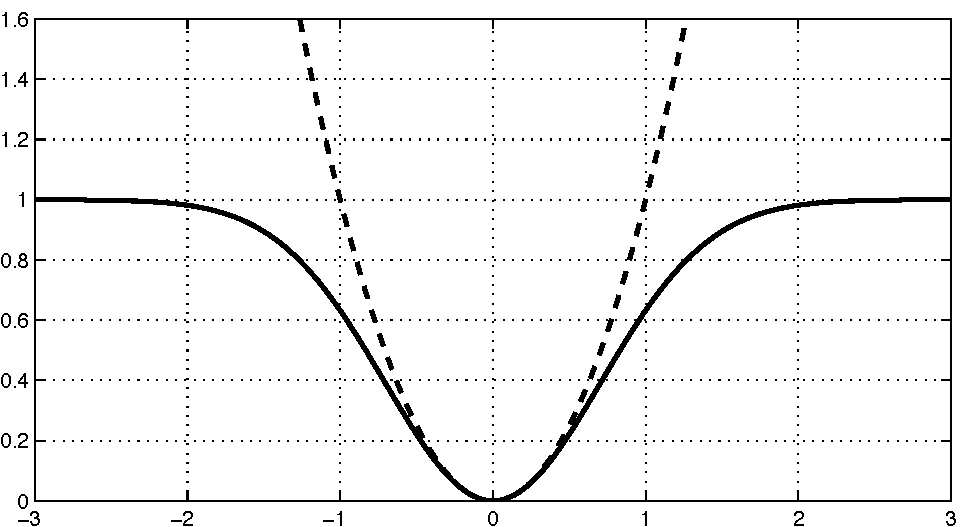
\includegraphics[scale=0.46,clip,trim=0.5cm 0.4cm 0cm 0cm]{figs/gpml/cost_costs.pdf}};
\node[rotate=90] at (-4.25,0) {Stage cost $c(\bz)$};
\node at (-3.8,0.4) {1};
\node at (0,-2.4) {State-action space $\bz$};
\node at (-2.25,-1.5) {\footnotesize Setpoint $\br$};
\path[line] (-1.4,-1.6) -- (-0.3,-1.87);
\end{tikzpicture}
%
\caption{Stage-costs for which the expectation in \Eq{costint} can be evaluated analytically for $\bz_k \sim \cN$. These functions are useful for penalising deviations of the state-action $\bz$ from a given setpoint $\br$. The quadratic is shown by the dashed line and the inverted-Gaussian is shown by the solid.}
\label{fig:cost_costs}
\end{figure}
%-------------------------------------------------------------------------------------------------------------------------------------------


Due to \Ass{moment}, the approximate distribution over state-action at each timestep is Gaussian $\bz_k \sim \cN$. In order to maintain an analytic evaluation problem, we require stage costs in which the expectation
\begin{equation} \label{eqn:costint}
\EE_{\bz_k}\big[c(\bz_k)\big] = \int c(\bz_k)p(\bz_k)\dd\bz_k
\end{equation}
can be evaluated analytically. If we desire to penalise the deviation of the state-action from some given setpoint $\br$ then the standard quadratic and the inverted squared exponential (or ``inverted-Gaussian") stage costs may be considered
\begin{align}
c_{\te{quad}}(\bz) &= \tfrac{1}{2}(\bz - \br)\T\bQ(\bz - \br) \label{eqn:cost_quad} \\
c_{\te{gauss}}(\bz) &= 1 - \exp\Big( - \tfrac{1}{2}(\bz - \br)\T\bQ(\bz-\br)\Big) \label{eqn:cost_gauss}
\end{align}
where $\bQ$ is a positive semi-definite weighting matrix. These are depicted in \Fig{cost_costs} which shows that close to $\br$ these functions are equivalent. The factor of a half is included in the definitions so that the $\bQ$ matrix can be interpreted as the covariance matrix of an unnormalised Gaussian and its elements tuned such that any state-action more than two standard-deviations away from the setpoint will incur a stage cost of approximately one. The inverted-Gaussian stage cost is locally quadratic and can be viewed as a saturated quadratic. The expectations of these costs are given as
\begin{align}
\EE_{\bz}\big[c_{\text{quad}}(\bz)\big] &= \half(\bm - \br)\T\bQ(\bm - \br) + \half\tr(\bS\bQ)
\label{eqn:Equad} \\[-0.3cm]
\EE_{\bz}\big[c_{\text{gauss}}(\bz)\big] &= 1 - \big|\bI + \bS\bQ\big|^{-\sha}
\exp\Big( -\half(\bm - \br)\T
\overbrace{ \bQ^{\sha}(\bI + \bQ^{\sha}\bS\bQ^{\sha})\inv\bQ^{\sha} }^{(\bQ\inv + \bS)\inv}
(\bm - \br)  \Big) \label{eqn:Egauss}
\end{align}
for $\bz \sim \cN(\bm,\bS)$. The use of the inverted-Gaussian stage cost leads to a useful behaviour in the context of probabilistic learning control.







\subsubsection{Natural Exploration-Exploitation}\label{sec:natexp}
The motivation for preferring the inverted-Gaussian stage cost \Eq{cost_gauss} over the conventional quadratic form in the context of learning control will now be outlined. Consider the optimal control problem posed in \Eq{Jcost} in which the initial state is known exactly $\bS_0 = \bO$ and the only source of uncertainty comes from the probabilistic model which is used to capture modelling uncertainty. As part of the offline simulation phase of the learning framework posed in \Sec{modelbased} now consider that the policy has to make a choice between two state-action densities $p_1(\bz)$ and $p_2(\bz)$ as shown in \Fig{exp_far}. If modelling uncertainty was ignored then the policy would favour the state distribution with mean closest to the setpoint $\br$ regardless of the uncertainty associated with the prediction. However, if uncertainty is taken into account, the policy will favour the more uncertain state with mean further from the setpoint since this has more density in the low cost region therefore yields a lower expected cost. 

The converse situation is depicted in \Fig{exp_near} where the probabilistic framework would favour policies that chose the more certain state despite the fact that its mean is further from the setpoint. 
This example illustrates that using a probabilistic model will lead to policies which drive the system into uncertain areas of its state-action space in high cost regions but favour cautious behaviour when close to the setpoint. This ``natural" exploration will aid the model learning process.



%-------------------------------------------------------------------------------------------------------------------------------------------
\begin{figure}[t]
\centering
\tikzstyle{line} = [draw, -latex]
\subfigure[Distributions with means far away from the setpoint]{
\begin{tikzpicture}
\small
\node at (0,0) {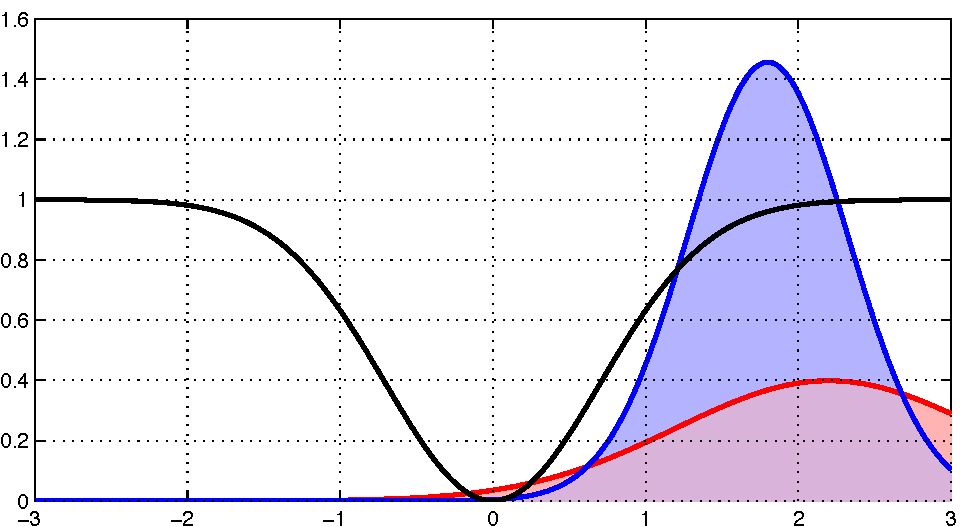
\includegraphics[scale=0.46,clip,trim=0.5cm 0.4cm 0cm 0cm]{figs/gpml/explore_far.pdf}};
\node at (0,-2.4) {State-action space $\bz$};
\node at (-3.0,0.75) {$c(\bz)$};
\node at (2.2,-0.3) {\color{blue}$p_1(\bz)$};
\node at (2.3,-1.55) {\color{red}$p_2(\bz)$};
\end{tikzpicture}
\label{fig:exp_far}
}
\hfill
\subfigure[Distributions with means close to the setpoint]{
\begin{tikzpicture}
\small
\node at (0,0) {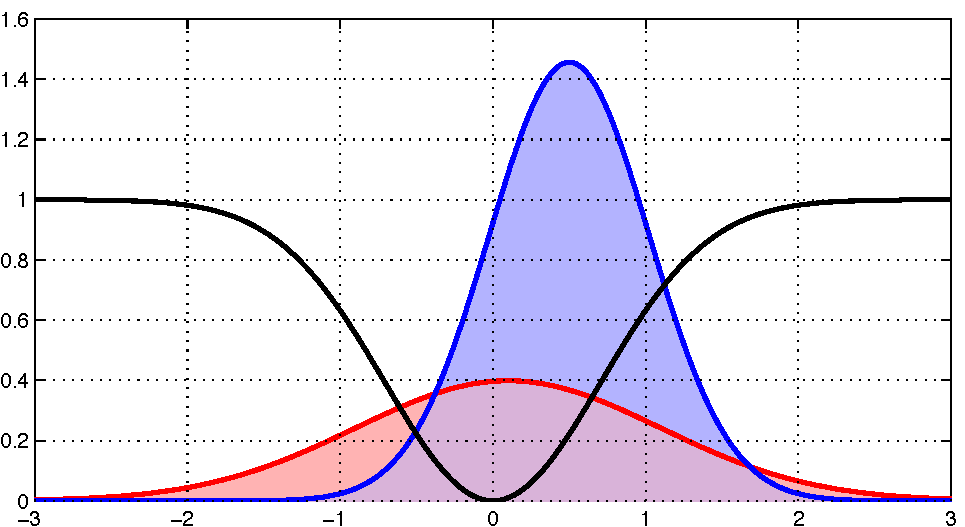
\includegraphics[scale=0.46,clip,trim=0.5cm 0.4cm 0cm 0cm]{figs/gpml/explore_near.pdf}};
\node at (0,-2.4) {State-action space $\bz$};
\node at (-3.0,0.75) {$c(\bz)$};
\node at (0.55,-0.1) {\color{blue}$p_1(\bz)$};
\node at (1.0,-1.7) {\color{red}$p_2(\bz)$};
\end{tikzpicture}
\label{fig:exp_near}
}
\caption{Illustration of how a ``natural" exploration of the state-action space can arise through use of an inverted-Gaussian stage cost. The stage cost is shown as a black line and two distributions over state-action space are shown by the blue and red curves, with the means shown explicitly.}
\end{figure}
%-------------------------------------------------------------------------------------------------------------------------------------------


The standard quadratic cost would not display this behaviour since the covariance of the state-action is always explicitly penalised by the additive term shown in \Eq{Equad}. Therefore the quadratic cost leads only to behaviour which seeks to exploit its current knowledge and not explore. It should be noted that this is not the standard exploration-exploitation tradeoff that appears in the reinforcement learning literature since this behaviour arises from being greedy with respect to a probabilistic model rather than explicitly applying random inputs.






\subsection{Policy Improvement}

Since an analytic approximation to the cost function in \Eq{learn1} is being considered, the gradient of this cost with respect to the policy parameters $\dd J(\bpsi)/\dd\bpsi$ can also be obtained in closed form. This means that we can make efficient use of gradient descent optimisation in order to carry out the improvement step of the simulation phase. The derivatives have the following structure
\begin{align}
\diff{J(\bpsi)}{\bpsi} &= \sum_{k=0}^{H} \diff{\EE_{\bz_k}\big[c(\bz_k)\big]}{\bpsi} 
\label{eqn:Jderiv1}
\end{align}
Due to the Gaussian assumption given in \Ass{moment}, the expectation of the stage cost $\EE_{\bz_k}\big[c(\bz_k)\big]$ is only dependant on the mean and variance of this distribution. Therefore the full derivative can be split up into partial derivatives
\begin{align}
\diff{\EE_{\bz_k}\big[c(\bz_k)\big]}{\bpsi} =
\pdiff{\EE_{\bz_k}\big[c(\bz_k)\big]}{\bm_k} \diff{\bm_k}{\bpsi} +
\pdiff{\EE_{\bz_k}\big[c(\bz_k)\big]}{\bS_k} \diff{\bS_k}{\bpsi}
\end{align}
where $\bm_{k} = \EE_{\bz_{k-1},\bff}[\bz_k|\bpi]$ and $\bS_{k} = \cov_{\bz_{k-1},\bff}[\bz_k|\bpi]$. The dimensions of these derivatives are defined according to the matrix calculus convention outlined in \App{matcal}. The derivatives of the mean and covariance at each step can be calculated in the following recursive manner
\begin{align}
\diff{\bm_k}{\bpsi} &= \pdiff{\bm_k}{\bm_{k-1}}\diff{\bm_{k-1}}{\bpsi} 
+ \pdiff{\bm_k}{\bS_{k-1}}\diff{\bS_{k-1}}{\bpsi} + \pdiff{\bm_k}{\bpsi} \\
\diff{\bS_k}{\bpsi} &= \pdiff{\bS_k}{\bm_{k-1}}\diff{\bm_{k-1}}{\bpsi} 
+ \pdiff{\bS_k}{\bS_{k-1}}\diff{\bS_{k-1}}{\bpsi} + \pdiff{\bS_k}{\bpsi}
\label{eqn:Jderiv2}
\end{align}
for $k \geq 1$ where each partial derivative is dependent on the type of dynamics model and policy structure used. The mean and covariance at $k=0$ can be partitioned as follows
\begin{align*}
\bm_0 &= \bmat{\bm_{\bx_0} \\ \bm_{\bu_0}}, 
&\bS_0 &= \bmat{\bS_{\bx_0} & \bS_{\bx\bu_0} \\ \bS_{\bx\bu_0}\T & \bS_{\bu_0}}
\end{align*}
where $\dd\bm_{\bx_0}/\dd\bpsi = \bO$ and $\dd\bS_{\bx_0}/\dd\bpsi = \bO$ since the initial state distribution is fixed.  The exact form of these derivatives depend on the form of the probabilistic model and the policy used. These calculations are implemented in an iterative fashion using MATLAB and can be found in \App{codeCost} implemented by the function \texttt{value.m}.























\section{State-Action Prediction} \label{sec:xuprediction}


%-------------------------------------------------------------------------------------------------------------------------------------------
\begin{figure}[t]
\centering
\tikzstyle{sum} = [circle, draw, minimum height=1cm]
\tikzstyle{block} = [rectangle, draw, fill=white, text width=7em, text centered, rounded corners, minimum height=4em]
\tikzstyle{line} = [draw, -latex]
%
\begin{tikzpicture}
	\small	
	\node at (-5.4,0.3) {$p(\bx_{k-1},\bu_{k-1})$};
	\node at (0,0.3) {$p(\bx_k)$};
	\node at (5.4,0.3) {$p(\bx_k,\bu_k)$};
	
	\node[block](dyn) at (-2.5,0) {Model \\$p(\bff|\cD,\hyp)$};
	\node[block](pol) at (2.5,0) {Policy \\$\bpi$};
	\path[line] (-6.8,0) -- (dyn.west); \node at (-7.5,0) {. . .};
	\path[line] (dyn.east) -- (pol.west);
	\path[draw] (pol.east) -- (6.8,0); \node at (7.5,0) {. . .};
	
\end{tikzpicture}
\caption{Propagation of uncertainty from a given state-action pair $(\bx_{k-1},\bu_{k-1})$ to the pair at the following timestep $(\bx_k,\bu_k)$ given a distribution over dynamics functions $p(\bff|\cD,\hyp)$ and the control policy $\bpi$.}
\label{fig:propxu}
\end{figure}
%-------------------------------------------------------------------------------------------------------------------------------------------

\subsection{Propagating Uncertainty}
Attention is now turned to the problem of inferring the assumed Gaussian distribution over state-action space $p(\bz_k)$ given the distribution at the previous timestep $p(\bz_{k-1}) \sim \cN$. This can then be cascaded in order to build up a distribution over the full trajectory $p(\btau)$. It would be useful to treat this problem in two stages as shown in \Fig{propxu}. First, find the distribution $p(\bx_k)$ using the probabilistic dynamics model $p(\bff|\cD,\hyp)$. Then find the joint distribution $p(\bx_k,\bu_k)$ using the policy $\bpi$. In order to do this, a tighter assumption is made:

\begin{ass}\label{ass:gauss}
Given $p(\bz_{k-1})$ is Gaussian, the resulting distribution of the next state-action $p(\bz_k)$ is replaced by the Gaussian distribution
\begin{equation*}
\bmat{\bx_k \\ \bu_k} \sim \cN\left(
\bmat{\EE_{\bz_{k-1},\bff}[\bx_k] \\ \EE_{\bchi_k}[\bu_k|\bpi]},
\bmat{\cov_{\bz_{k-1},\bff}[\bx_k] & \cov_{\bchi_k}[\bchi_k,\bu_k|\bpi] \\
\cov_{\bchi_k}[\bu_k,\bchi_k|\bpi] & \cov_{\bchi_k}[\bu_k|\bpi]}
\right)
\end{equation*}
where $p(\bchi_k)$ is the moment matched approximation of the real distribution $p(\bx_k)$.
%Given $p(\bz_{k-1}) \sim \cN$, the distribution of the next state $p(\bx_k)$ is Gaussian with mean $\EE_{\bz_{k-1},\bff}[\bx_k]$ and covariance $\cov_{\bz_{k-1},\bff}[\bx_k]$. Additionally, the joint distribution $p(\bz_{k-1},\bx_k) \sim \cN$ is also Gaussian with cross covariance $\cov_{\bz_{k-1},\bff}[\bz_{k-1}, \bx_k|\bpi]$.
\end{ass}

Note that \Ass{moment} uses the real distribution $p(\bx_k)$ as the input to the control policy whereas \Ass{gauss} uses the moment matched approximation $p(\bchi_k)$. From now on, no distinction will be made between the real distribution $p(\bx)$ and its approximation $p(\bchi)$.
%Therefore, given Assumptions \ref{ass:moment} and \ref{ass:gauss} the distribution of $\bz_k$ given $\bz_{k-1}$ can be partitioned as
%\begin{equation}
%\bmat{\bx_k \\ \bu_k} \sim \cN\left(
%\bmat{\EE_{\bz_{k-1},\bff}[\bx_k] \\ \EE_{\bx_k}[\bu_k|\bpi]},
%\bmat{\cov_{\bz_{k-1},\bff}[\bx_k] & \cov_{\bx_k}[\bx_k,\bu_k|\bpi] \\
%\cov_{\bx_k}[\bu_k,\bx_k|\bpi] & \cov_{\bx_k}[\bu_k|\bpi]}
%\right)
%\label{eqn:jointgauss}
%\end{equation}






\subsection{Gaussian Approximation Schemes}
The use of the moment matching scheme given in Assumptions \ref{ass:moment} and \ref{ass:gauss} will now be motivated. For now, consider the propagation of uncertainty from the input $\bz \sim \cN(\bm,\bS)$ through a distribution over functions $p(\bff)$ to the next state $\bff(\bz)$. In this case we assume that the probabilistic model returns a Gaussian distribution when queried at a deterministic input. This is the first step shown in \Fig{propxu}. There are a number of methods available for approximating the real distribution $p\big(\bff(\bz)\big)$ with a Gaussian $\cN(\bm_*,\bS_*)$. We shall briefly introduce a number of these methods now
%
\begin{enumerate}
\item {\bf Taylor Series Expansions.} Approximate the dynamics $p(\bff)$ with a finite Taylor series expansion of the real nonlinear equations about the input mean $\bm$. Then for a first order expansion for example we have 
\begin{align*}
\bm_* &= \EE_{\bff}[\bff(\bm)] 
&\bS_* &= \big( \partial\EE_{\bff}[\bff(\bm)]/\partial\bm \big)^2 + \cov_{\bff}[\bff(\bm)]
\end{align*}
This is equivalent to taking linearisations, which is the method that is used in the prediction step of the Extended Kalman Filter (EKF). See Chapter 8 of \cite{AnMo79} for more information on the EKF.
%
\item {\bf Unscented Transformation.} Instead of making assumptions about the structural nature of the dynamics model or policy, the unscented transformation takes a finite number of (weighted) ``sigma-points" $\cS = \{\hat\bz_{1} \dots \hat\bz_{S}\}$ with the same second-order statistics as $p(\bz)$. Mathematically
$\EE_{\bz}[\bz] = \sum_{s=1}^S W_s\hat\bz_{s}$ and $\cov_{\bz}[\bz] = \sum_{s=1}^S W_s(\hat\bz_{s}-\EE_{\bz}[\bz])(\hat\bz_{s}-\EE_{\bz}[\bz])\T$
where $\sum_{s=1}^S W_s=1$, $W_s > 0$. It then maps them through the mean of the probabilistic dynamics model to obtain the transformed set $\EE_{\bff}[\bff(\cS)] = \{\EE_{\bff}[\bff(\hat\bz_{1})] \dots \EE_{\bff}[\bff(\hat\bz_{S})]\}$. The mean and covariance are then set to that of the (weighted) statistics of the transformed data set
\begin{align*}
\bm_* &= \sum_{s=1}^S W_s\EE_{\bff}[\bff(\hat\bz_{s})] 
&\bS_* &= \sum_{s=1}^S W_s\big(\EE_{\bff}[\bff(\hat\bz_{s})]-\bm_*\big)\big(\EE_{\bff}[\bff(\hat\bz_{s})]-\bm_*\big)\T
+ \cov_{\bff}[\bff(\bm)]
\end{align*}
respectively to give an unbiased prediction. This method was proposed as the prediction step of the Unscented Kalman Filter (UKF) of \cite{JU97}.
%
\item {\bf Exact Moment Matching.} In situations where they are possible to obtain, the moment matching approximation finds the exact mean and covariance 
\begin{align*}
\bm_* &= \EE_{\bz,\bff}[\bff(\bz)]
& \bS_* &= \cov_{\bz,\bff}[\bff(\bz)]
\end{align*}
of the actual distribution $p\big(\bff(\bz)\big)$. To complete the filtering parallel of the previous two examples, the moment matching technique is used in the prediction step of an Assumed Density Filter (ADF). See Chapter 12 of \cite{May82} for more information on the ADF.
\end{enumerate}


%-------------------------------------------------------------------------------------------------------------------------------------------
\begin{figure*}
\centering
\footnotesize
\subfigure[Linear approximation. Linearisations of the function about the state-action mean $\EE{[\bz]}$ are shown.]{
\tikzstyle{line} = [draw, -latex]
\begin{tikzpicture}
\node at (-7.4,-3) {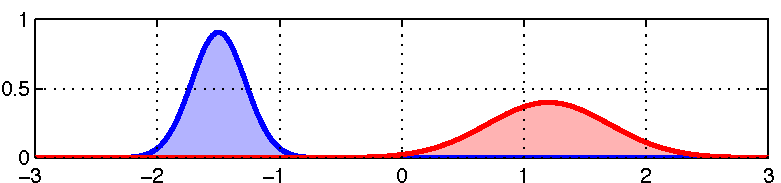
\includegraphics[scale=0.6, clip, trim=0.5cm 0.4cm 0cm 0cm]{figs/gpml/propLIN_1.pdf}};
\node at (-7.4,0) {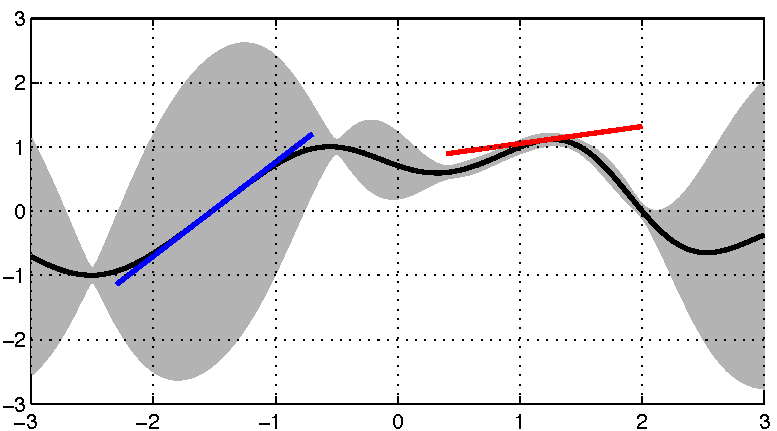
\includegraphics[scale=0.6, clip, trim=0.5cm 0.4cm 0cm 0cm]{figs/gpml/propLIN_2.pdf}};
\node at (0,0) {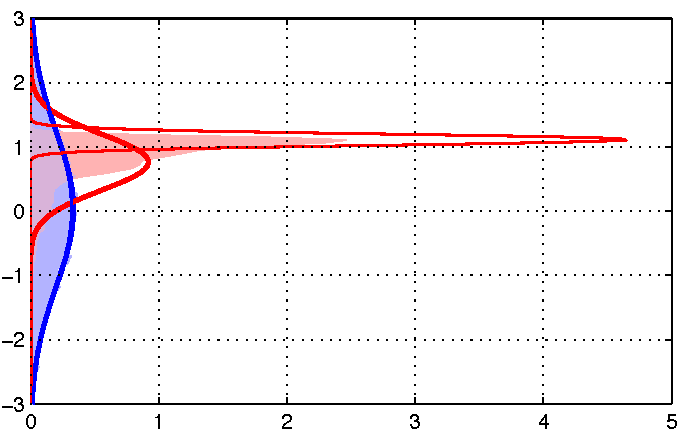
\includegraphics[scale=0.6, clip, trim=0.5cm 0.4cm 0cm 0cm]{figs/gpml/propLIN_3.pdf}};

\node at (-8.3,-3) {\color{blue} $p_1(\bz)$};
\node at (-5,-3) {\color{red} $p_2(\bz)$};
\node[rotate=90] at (-11.5,0) {Function distribution};
\node at (-10.5,1.55) {$p(\bff)$};
\node at (-2.4,-1.1) {\color{blue} $q_1\big(\bff(\bz)\big)$};
\node at (-1.3,0.2) {\color{red} $q_2\big(\bff(\bz)\big)$};

\draw[rounded corners,fill=white] (-0.5,-1.85) rectangle (3,-0.25);
\node[fill=blue!30,circle,minimum height=0.33cm] at (-0.2,-0.65) {};
\node[fill=red!30,circle,minimum height=0.33cm] at (0.15,-0.65) {};
\draw[very thick,blue] (-0.35,-1.08) -- (-0.05,-1.08); \draw[very thick,red] (0.0,-1.08) -- (0.3,-1.08);
\draw[thin,blue] (-0.35,-1.48) -- (-0.05,-1.48); \draw[thin,red] (0.0,-1.48) -- (0.3,-1.48);
\node[anchor=west] at (0.35,-0.65) {Monte Carlo};
\node[anchor=west] at (0.35,-1.05) {Exact Moments};
\node[anchor=west] at (0.35,-1.45) {\bf Linearised};

\end{tikzpicture}
\label{fig:propLinUnsA}
}
%
\subfigure[Unscented transformation. Sigma points $\cS$ along with their projections $\bff(\cS)$ and weights $W$ are shown.]{
\tikzstyle{line} = [draw, -latex]
\begin{tikzpicture}
\node at (-7.4,-3) {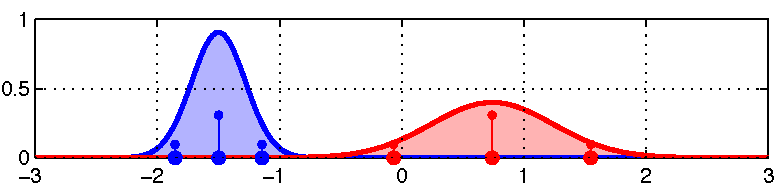
\includegraphics[scale=0.6, clip, trim=0.5cm 0.3cm 0cm 0cm]{figs/gpml/propUNS_1.pdf}};
\node at (-7.4,0) {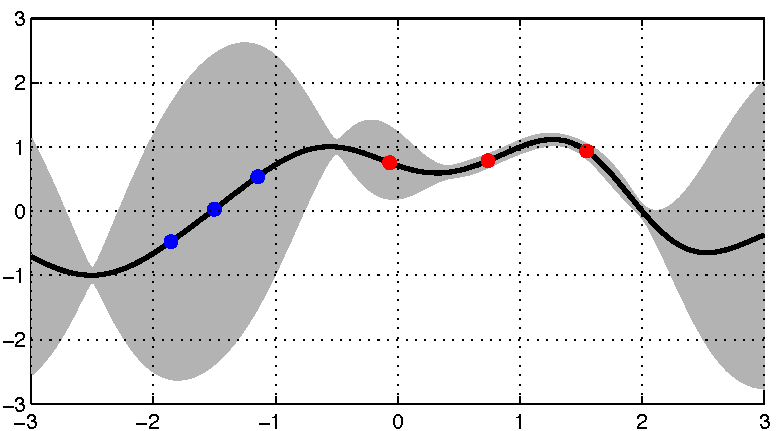
\includegraphics[scale=0.6, clip, trim=0.5cm 0.4cm 0cm 0cm]{figs/gpml/propUNS_2.pdf}};
\node at (0,0) {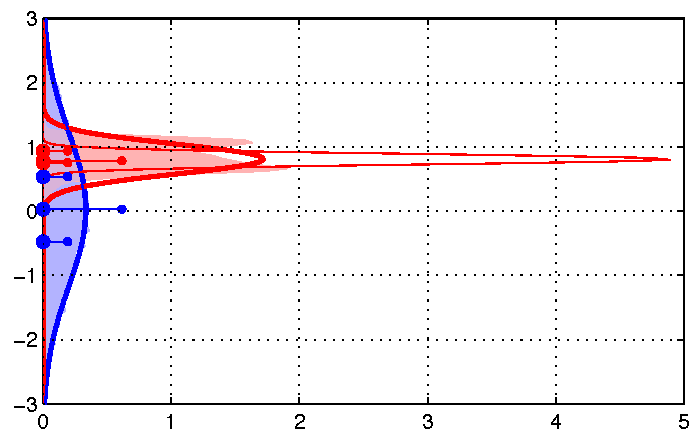
\includegraphics[scale=0.6, clip, trim=0.6cm 0.4cm 0cm 0cm]{figs/gpml/propUNS_3.pdf}};

\node at (-8.3,-3) {\color{blue} $p_3(\bz)$};
\node at (-5,-3) {\color{red} $p_4(\bz)$};
\node[rotate=90] at (-11.5,0) {Function distribution};
\node at (-10.5,1.55) {$p(\bff)$};
\node at (-2.4,-1.1) {\color{blue} $q_3\big(\bff(\bz)\big)$};
\node at (-1.2,0.0) {\color{red} $q_4\big(\bff(\bz)\big)$};

\draw[rounded corners,fill=white] (-0.5,-1.85) rectangle (3,-0.25);
\node[fill=blue!30,circle,minimum height=0.33cm] at (-0.2,-0.65) {};
\node[fill=red!30,circle,minimum height=0.33cm] at (0.15,-0.65) {};
\draw[very thick,blue] (-0.35,-1.08) -- (-0.05,-1.08); \draw[very thick,red] (0.0,-1.08) -- (0.3,-1.08);
\draw[thin,blue] (-0.35,-1.48) -- (-0.05,-1.48); \draw[thin,red] (0.0,-1.48) -- (0.3,-1.48);
\node[anchor=west] at (0.35,-0.65) {Monte Carlo};
\node[anchor=west] at (0.35,-1.05) {Exact Moments};
\node[anchor=west] at (0.35,-1.45) {\bf Unscented};
\end{tikzpicture}
\label{fig:propLinUnsB}
}
\caption{Propagation of uncertainty through a deterministic mapping $\bff$ using linearisation, the unscented transformation and exact moment matching. The lower plots show two distributions over $\bz$. The central plot shows the stochastic function $\bff$ with mean shown by the solid line and the 2$\sigma$ uncertainty region in gray. The right hand plot shows the true output distributions (obtained by sampling) and the various approximation schemes. Fig.$\!$ (a) is an example of the degeneracy of the linearised approximation and Fig.$\!$ (b) shows the degeneracy of the unscented transform.}
\label{fig:propLinUns}
\end{figure*}
%-------------------------------------------------------------------------------------------------------------------------------------------


%-------------------------------------------------------------------------------------------------------------------------------------------
%\begin{figure}[t]
%\centering
%\subfigure[Linear approximation. Linearisations of the function about the state-action mean $\EE{[\bz]}$ are shown.]{
%\tikzstyle{line} = [draw, -latex]
%\begin{tikzpicture}
%\scriptsize
%\node at (0,0) {\includegraphics[width=0.45\textwidth, clip, trim=1cm 0cm 0cm 0cm]{figs/gpml/propLin.pdf}};
%\draw[fill=white,white] (1.4,-2.1) rectangle (1.6,-0.8);
%\path[line] (-3.58,-2.13) -- (-3.58,-1.0); \path[line] (-3.68,-2.03) -- (1,-2.03); % bottom
%\path[line] (-3.58,-0.9) -- (-3.58,2.2); \path[line] (-3.68,-0.8) -- (1,-0.8); % middle
%\path[line] (1.47,-0.9) -- (1.47,2.2); \path[line] (1.37,-0.8) -- (3.5,-0.8); % right
%\node at (0.7,-0.55) {$\bz$}; \node at (-3.17,-1.2) {$p(\bz)$};
%\node at (-3.2,1.95) {$\bff(\bz)$}; %\node at (0.8,-1.0) {$\bz$};
%\node at (3.0,-0.5) {$p\big(\bff(\bz)\big)$};
%\end{tikzpicture}
%\label{fig:propLinUnsA}
%}
%
%\hfill
%
%\subfigure[Unscented transformation. Sigma points $\cS$ along with their projections $\bff(\cS)$ and weights $W$ are shown.]{
%\tikzstyle{line} = [draw, -latex]
%\begin{tikzpicture}
%\scriptsize
%\node at (0,0) {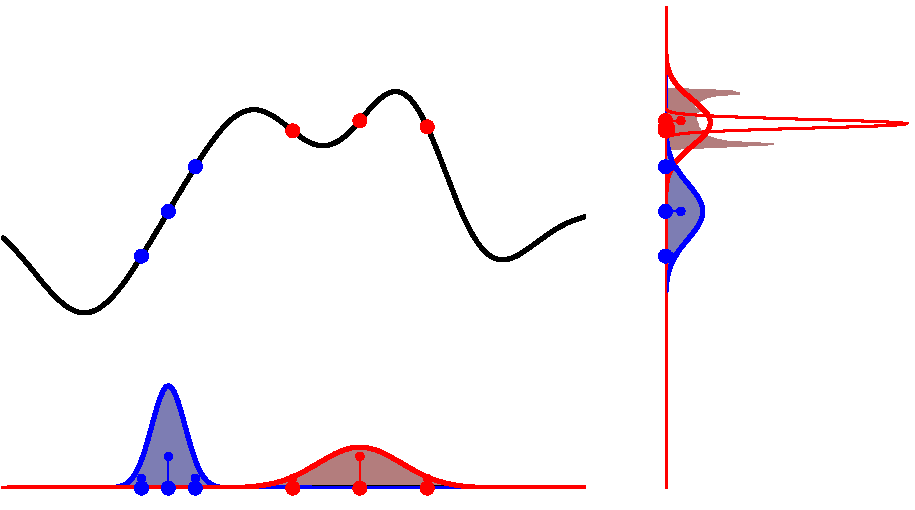
\includegraphics[width=0.45\textwidth, clip, trim=1cm 0.2cm 0cm 0cm]{figs/gpml/propUns.pdf}};
%\draw[fill=white,white] (1.4,-2.1) rectangle (1.6,-0.8);
%\path[line] (-3.58,-2.115) -- (-3.58,-1.0); \path[line] (-3.68,-2.015) -- (1,-2.015); % bottom
%\path[line] (-3.58,-0.9) -- (-3.58,2.2); \path[line] (-3.68,-0.8) -- (1,-0.8); % middle
%\path[line] (1.5,-0.9) -- (1.5,2.2); \path[line] (1.4,-0.8) -- (3.5,-0.8); % right
%\node at (0.7,-0.55) {$\bz$}; \node at (-3.17,-1.2) {$p(\bz)$};
%\node at (-3.2,1.95) {$\bff(\bz)$}; %\node at (0.8,-1.0) {$\bz$};
%\node at (3.0,-0.5) {$p\big(\bff(\bz)\big)$};
%\end{tikzpicture}
%\label{fig:propLinUnsB}
%}
%\caption{Propagation of uncertainty through a deterministic mapping $\bff$ using linearisation about the mean of the state-action distribution, the unscented transformation and an exact moment matching approach. The lower plot shows two input distributions over $\bz$. The central plot shows the mapping underlying function $\bff$. The right hand plot shows Monte-Carlo approximations of the real output distributions (shaded), and moment matched (thick solid) Gaussian approximations. Plot (a) shows two examples of the linearised approximation (thin solid) where the red example is approaching degeneracy. Plot (b) shows two examples of the unscented transformation (thin solid) where the red example is approaching degeneracy.}
%\label{fig:propLinUns}
%\end{figure}
%-------------------------------------------------------------------------------------------------------------------------------------------




%
Both the Taylor series expansion and the unscented transformation methods can potentially suffer from degeneracy as demonstrated in \Fig{propLinUns}. In the cases depicted by the blue distributions the function $\bff$ is close to linear in the region where the distribution has high density and therefore all methods make good approximations to the actual distribution. An example of the degeneracy of the linear approximation is shown by the red plot in \Fig{propLinUnsA} where the gradient approaches zero and the output distribution approaches the delta distribution and ignores much of the mass of the real output distribution. Similarly, the potential degeneracy of the unscented transformation is demonstrated in the red case shown in \Fig{propLinUnsB}. A further example is given in \cite{DTHH12}. 

The moment matching approach does not suffer from degeneracy for obvious reasons. We further note that the moment matching approach is, in a sense, a conservative approximation. In order to appreciate this, consider the 
Kullback-Leibler (KL) divergence $\mathrm{KL}\big(q || p\big)$ of the underlying distribution $p$ with respect to some Gaussian distribution $q$. We can prove that the Gaussian which minimises this divergence is the moment matched solution. For details of this proof see \App{KLdiv}. 
%
The nature of the KL divergence ensures that the approximate distribution $q$ is non-negligible where the real distribution $p$ is non-negligible, but not the other way around. In this sense the predictions will be conservative.

The advantage of using a Taylor series or unscented transformation based method is that they can be applied to a broader class of systems whereas the moment matching assumption is more restrictive. However, since a very useful set of models is amenable to the moment matching approach this was the method that has been adopted in this thesis.



\subsection{Modelling Uncertainty}
In a learning context it is important to treat modelling uncertainty in a rigorous manner. This is readily handled in a Bayesian framework. Given a parametric representation of the dynamics consisting of a linear sum of appropriate basis functions the Bayesian framework provides a way of making predictions based on a prior distribution over parameters and an observed data set.


% Further, it would be preferable not to impose a full parametric structure on the form of the dynamics that are to be modelled as this process can often be based on oversimplifying assumptions. Rather, it would be good to make predictions based on observed data and some higher level assumptions regarding the structure of the dynamics, such as smoothness or some intrinsic length-scale. These issues are well handled by the nonparametric probabilistic modelling framework of Gaussian processes.
















\section{Bayesian Modelling} \label{sec:bayesmodelling}%%%%%%%%%%%%%%%%%%%%%%%%%%%%%%%%

\subsection{Problem Outline} \label{sec:bayesproblem}
This section considers the problem of finding a probabilistic model $p(\bff|\cD, \hyp)$ defining a distribution over the function space, given some training data set $\cD$ and hyperparameters $\hyp$ and using this model to make predictions. This problem can be addressed by a Bayesian method known as Gaussian Processes (GPs). A Gaussian process  is defined by \cite{RaWi06} in \Def{GP}.

\begin{defin}[Gaussian process] \label{def:GP}
A collection of random variables, any finite number of which have a joint Gaussian distribution.
\end{defin}
%
Informally speaking, GPs are a means of placing a prior over a space of functions $p(\bff|\hyp)$ from which samples can be drawn, an extension of the idea of multivariate Gaussian distributions to infinitely long vectors, or functions. Once training data has been observed, this can be updated to a posterior distribution $p(\bff|\cD,\hyp)$ which is the probabilistic model required by the learning framework outlined in \Sec{learnover}.
%
Given a deterministic input $\bz$, GPs provide a predictive Gaussian distribution over possible next states with mean $\EE_{\bff}[\bff(\bz)|\bz,\cD]$ and covariance $\cov_{\bff}[\bff(\bz)|\bz,\cD]$. Explicit dependence on the hyperparameters $\hyp$ will be dropped from now on for clarity. However, from \Sec{xuprediction}, making predictions with respect to uncertain $\bz \sim \cN$ is required for the moment matching framework. In other words, making predictions of the mean $\EE_{\bz,\bff}[\bff(\bz)|\cD]$ and covariance $\cov_{\bz,\bff}[\bff(\bz)|\cD]$.



%In order to motivate their relevance in this context, a parametric approach to modelling will be considered which will to a full nonparametric framework. First, the form of the training data set $\cD$ must be considered.

Now the exact form of the training data set $\cD$ will be discussed. Data will be given in the form of $n$ state-actions and next-state pairs
\begin{align}
\bZ &= \bmat{ \bx_{k_1}\T & \bu_{k_1}\T \\ \vdots & \vdots \\ \bx_{k_n}\T & \bu_{k_n}\T} \in \RR^{n \times D} &\text{and}
&& \bY &= \bmat{ \bx_{k_1+1}\T \\ \vdots \\ \bx_{k_n+1}\T } \in \RR^{n\times E} \label{eqn:cZY}
\end{align}
for $-\infty < k_1 < \dots < k_n < 0$ not necessarily sampled consecutively. For the purposes of the following discussion, state-action pairs are referred to as ``inputs" and the next-states are referred to as ``outputs". Now, an important issue arises here. In reality all of these measurements will be corrupted by noise, normally assumed to be additive Gaussian noise. However, the GP framework assumes that only the outputs $\bY$ are corrupted by additive noise $\be \sim \cN(\bO, \bS_{\be})$ with diagonal covariance $\bS_{\be}$ and uncorrelated between timesteps but the inputs are noise free. The GP approach to a fully noisy data set will be discussed later, but for now this assumption will be made. Therefore, the noisy output measurements will be referred to by $\bY$, while the noise-free set is referred to by the matrix $\bF$.
%where $\by = \bx + \be$ are state measurements corrupted by noise  The underlying values of the next-states are stored in the matrix $\bF = \big[\bx_{t_1+1} \dots \bx_{t_n+1} \big]$. In this framework it is assumed that the underlying state is available in order to form the $\bZ$ matrix. %This assumption may of course be unrealistic and is addressed formally by \cite{MR11} who consider the case of noisy input values in a Gaussian process framework. 

It is worthy of note that the following presentation of Gaussian process theory is novel in the sense that we deal with the multivariate case from the very outset. Most textbooks and presentations of the fundamental theory talk about the multivariate case as an afterthought.







\subsection{Parametric Approach}
\subsubsection{Prior}
The linear parametric approach assumes that the unknown function $\bff: \RR^D \rightarrow \RR^E$ belongs to the set of functions parameterised by
\begin{equation}
\bff(\bz) = \bPh(\bz)\T \bw    \label{eqn:param}
\end{equation}
where $\bw \in \RR^{P}$ is a vector of weights and the feature matrix $\bPh(\bz) \in \RR^{P\times E}$ is made up of a number of basis functions. Note that the feature matrix is often of a form such that there are no cross correlations between output dimensions through common weights. In other words $\bPh(\bz) = \bI \otimes \bph(\bz)$. The feature matrix is defined to handle matrix inputs by defining the following convention
\begin{align}
\bPh(\bZ) &:= \bmat{ \Phi[:,1](\bZ) & \dots & \Phi[:,E](\bZ) } \in \RR^{P \times En}
\label{eqn:Phi1} \\
\Phi[:,i](\bZ) &:= \bmat{ \Phi[:,i](\bz_{k_1}) & \dots & \Phi[:,i](\bz_{k_n}) } \in \RR^{P \times n}
\label{eqn:Phi2}
\end{align}
 where $\Phi[:,i](\bz)$ is the $i\tth$ column of $\bPh(\bz)$. Note that the standard linear dynamics model $\bff(\bz) = \bA\bx +\bB\bu$ falls under this model class by setting $\bPh(\bz) = \bI \otimes \bz$ and $\bw = \vect\big([\bA \;\bB]\T\big)$. In a Bayesian framework a prior distribution is placed over the unknown parameter space $p(\bw|\hyp) = \cN(\bet,\bOm)$ which is defined in terms of the hyperparameters $\hyp = \{\bet,\bOm\}$ and represents any prior knowledge regarding their relationship. 

This prior over parameters leads to a prior over the space of functions $p(\bff|\hyp)$ which satisfies the definition of a Gaussian process. The GP is parameterised by a \textit{mean function} and \textit{covariance function} (or \textit{kernel}) defined to be
\begin{align}
\bmm(\bz) &:= \EE_{\bw}\big[\bff(\bz)\big] &&
\!\!\!\!\!\!\!\!\!\!\!\!\!\!\!\!\!\!\!\!\!\!\!\!\!\!\!\!\!\!\!\!\!\!\!\!\!\!\!\!\!\!\!\!\!\!\!\!\!\!\!\!\!\!\!\!\!\!\!\!
= \bPh(\bz)\T\bet \\
\bK(\bz,\tilde\bz) &:= \cov_{\bw}\big[\bff(\bz), \bff(\tilde\bz)\big] &&
\!\!\!\!\!\!\!\!\!\!\!\!\!\!\!\!\!\!\!\!\!\!\!\!\!\!\!\!\!\!\!\!\!\!\!\!\!\!\!\!\!\!\!\!\!\!\!\!\!\!\!\!\!\!\!\!\!\!\!\!
= \bPh(\bz)\T \bOm \bPh(\tilde\bz) \label{eqn:covfunc}
\end{align}
respectively. These functions are also defined to take matrix inputs with dimensions determined through the way in which matrix inputs are handled by $\bPh$. For example, if $\bPh(\bz) = \bI \otimes \bph(\bz)$ the covariance matrix $\bK(\bZ,\bZ)$ would be block diagonal, with one block per output dimension. For notational convenience we shall now define $\bK_{nn}:=\bK(\bZ,\bZ)$. The covariance function can also accept a single input by letting $\bK(\bz) := \bK(\bz,\bz)$. Zero mean priors $\bet = \bO$ shall be considered for the remainder of this discussion in order to keep the notation uncluttered, however extension to $\bet \neq \bO$ is trivial.





%-------------------------------------------------------------------------------------------------------------------------------------------
\begin{figure}[t]
\centering
\small
\subfigure[Samples from the prior $p(\bff|\hyp)$.]{
\tikzstyle{line} = [draw, -latex]
\begin{tikzpicture}
	\node at (0,0) {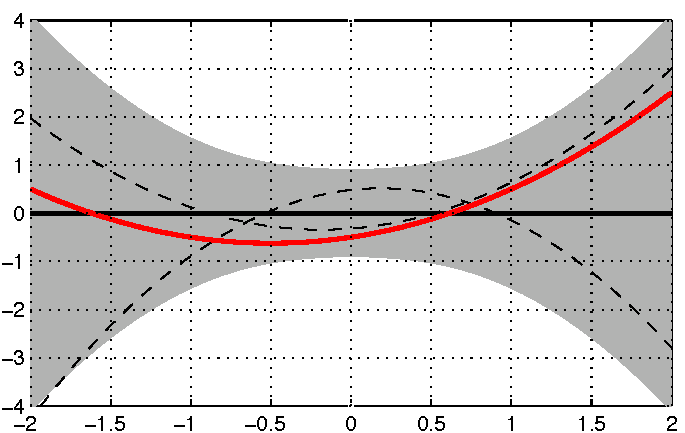
\includegraphics[scale=0.67, clip, trim = 0.5cm 0.45cm 0.2cm 0cm]{figs/gpml/priorRBF.pdf}};
	\node at (3.2,-2.05) {$\bz$};
	\node at (-3.2,1.75) {$\bff(\bz)$};
\end{tikzpicture}
}
\hfill
\subfigure[Samples from the posterior $p(\bff|\cD,\hyp)$.]{
\tikzstyle{line} = [draw, -latex]
\begin{tikzpicture}
	\node at (0,0) {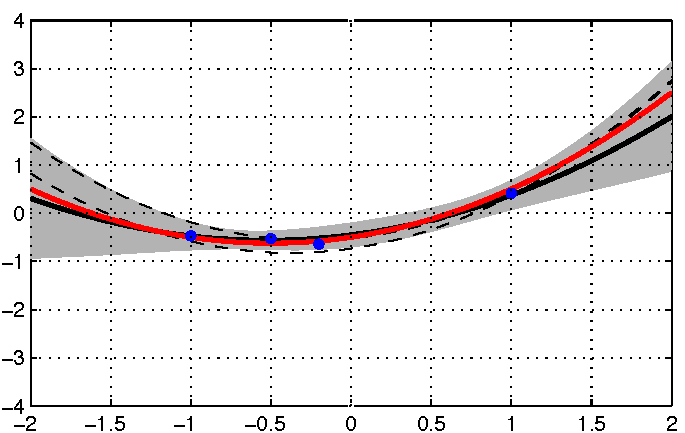
\includegraphics[scale=0.67, clip, trim = 0.5cm 0.45cm 0.2cm 0cm]{figs/gpml/postRBF.pdf}};
	\node at (3.2,-2.05) {$\bz$};
	\node at (-3.2,1.75) {$\bff(\bz)$};
\end{tikzpicture}
}
\caption{Samples from a prior and posterior distribution over quadratic functions $\bff(\bz) = \bPh(\bz)^\top\bw$ where $\bph(\bz) = \big[1; \bz; \vect(\bz\bz^\top)\big]$ with prior Gaussian distribution over the weights $p(\bw|\hyp) = \cN(\bO,\bOm)$.  The red, black and dashed lines show the underlying function $\bff$, mean of the distribution over functions (prior $\bmm$ and posterior $\bmm_+$) and sampled functions respectively. The grey regions denote two standard deviations, or 95\% confidence region, of the distribution. Training data is shown as blue dots on the posterior plot.}
\label{fig:linearprior}
\end{figure}
%-------------------------------------------------------------------------------------------------------------------------------------------




\subsubsection{Posterior}
The posterior over parameters given the observed data set $\cD$ is computed using Bayes' rule
\begin{equation}
p(\bw|\cD,\hyp) = \frac{p(\bY|\bw,\bZ,\hyp)}{p(\bY|\bZ,\hyp)} p(\bw|\hyp)
\end{equation}
where $p(\bY|\bw,\bZ,\hyp)$ is the \textit{likelihood} of the data given the parameters and $p(\bY|\bZ,\hyp)$ is the \textit{marginal likelihood} (or \textit{evidence}) since it is the likelihood of the data marginalised over the parameters $ p(\bY|\bZ,\hyp) = \int p(\bY|\bw,\bZ,\hyp) p(\bw|\hyp) \dd\bw$. Note that the prior over parameters is independent of the training input set therefore $p(\bw|\hyp) = p(\bw|\bZ,\hyp)$.
%
Given that the likelihood and the prior are simply multivariate Gaussians, their product can be calculated analytically as
\begin{align}
p(\bw|\cD,\hyp) &\propto  p(\bY|\bw,\bZ,\hyp) p(\bw|\hyp) 
= \cN\Big( \bPh(\bZ)\T \bw, \bS_{\be}\otimes\bI \Big)  \cN(\bet,\bOm)
\end{align}
where the product is an unnormalised Gaussian which can be found using the identity given in \App{gauss}. It is assumed that the additive noise covariance $\bS_{\be}$ is also a hyperparameter to be inferred. By normalising this product, the posterior over parameter space is given in closed form as $p(\bw|\cD,\hyp) = \cN(\bet_+, \bOm_+)$ with mean and covariance
\begin{align}
\bet_+ &= \Big( \bOm^{-1} + \bPh(\bZ)( \bS_{\be}\otimes\bI)^{-1}\bPh(\bZ)\T \Big)^{-1}\bPh(\bZ)( \bS_{\be}\otimes\bI)^{-1}\vec\bY \label{eqn:parampostM}\\
\bOm_+ &= \Big( \bOm^{-1} + \bPh(\bZ)( \bS_{\be}\otimes\bI)^{-1}\bPh(\bZ)\T \Big)^{-1} \label{eqn:parampostV}
\end{align}
Since the distribution is Gaussian, the mean $\bet_+ = \EE[\bw|\cD,\hyp]$ is the Maximum A Posteriori (MAP) estimate of the parameters $\bw$.  It follows that the posterior distribution over function space $\bff|\cD \sim \mathcal{GP}\big(\bmm_+, \bK_+\big)$ is also a Gaussian process with mean function and covariance function
\begin{align}
\bmm_+(\bz) &= \bPh(\bz)\T\bet_+ \label{eqn:rbfM} \\
\bK_+(\bz,\tilde\bz) &= \bPh(\bz)\T \bOm_+ \bPh(\tilde\bz) \label{eqn:rbfV}
\end{align}
An example of sampling from the prior and posterior of a single-input single-output quadratic function is shown in \Fig{linearprior}. Prediction is then achieved simply as $p\big(\bff(\bz)|\bz,\cD,\hyp\big) = \cN\big(\bmm_+(\bz), \bK_+(\bz) \big)$.

It is instructive to note that as the prior becomes ``flat", $\bOm =\omega\bI$ as $\omega\rightarrow \infty$, the posterior mean prediction tends to $\bet_+ \rightarrow \big(\bPh(\bZ)\bPh(\bZ)\T\big)^{-1}\bPh(\bZ)\vec\bY$. This is the solution of the linear least squares problem $\bPh(\bZ)\T\bp = \vec\bY$. A flat prior implies that the MAP estimate is the same as the Maximum Likelihood estimate since $p(\bw|\cD,\hyp) \propto p(\bY|\bw,\bZ,\hyp)$.






\subsubsection{Kernel Trick} 
The expressions for the posterior mean and covariance in \Eqs{rbfM}{rbfV} can be manipulated into an equivalent form given in \Theo{kerneltrick}. This is a well known result in the Machine Learning community and is based on \textit{Mercer's Theorem}, see \cite{Mer1909}. As will be shown in the following section, these are actually the predictive equations for a Gaussian process. 

\begin{theo}[Kernel Trick] \label{theo:kerneltrick}
%
The expressions for the posterior mean and covariance function in \Eqs{rbfM}{rbfV} are equivalent to 
\begin{align}
\bmm_{+}(\bz) &= \bK(\bz,\bZ) \Big(\bK_{nn}+\bS_{\be}\otimes\bI\Big)^{-1} \vec\bY  \label{eqn:rbfM2} \\
\bK_{+}(\bz,\tilde\bz) &= \bK(\bz,\tilde\bz) - 
\bK(\bz,\bZ) \Big(\bK_{nn}+\bS_{\be}\otimes\bI\Big)^{-1}\bK(\bZ,\tilde\bz) \label{eqn:rbfV2}
\end{align}
where the kernel matrices $\bK$ consist of inner products of the feature matrix $\bPh$ with respect to the prior covariance $\bOm$ as defined in \Eq{covfunc}.
%
\spa \end{theo}

\begin{proof}
Let $\bA = \bOm$, $\bB = \bS_{\be}\otimes\bI$ and $\bC = \bPh(\bZ)$.  Then the parameter mean $\bet_+$ from \Eq{parampostM} can be written as
\begin{align*}
\bet_+ &= \big( \bA^{-1} + \bC\bB\inv\bC\T \big)^{-1} \bC\bB\inv \vec\bY \\
&= \bA\bC \big(  \bC\T\bA\bC + \bB \big)^{-1} \vec\bY \\
&= \bOm\bPh(\bZ) \Big( \bPh(\bZ)\T\bOm\bPh(\bZ) + \bS_{\be}\otimes\bI \Big)^{-1}  \vec\bY
\end{align*}
which follows from a variant of the matrix inversion lemma\footnote{$(\bP\inv + \bR\bQ\inv\bR\T)\inv\bR\bQ\inv = \bP\bR\T(\bR\T\bP\bR + \bQ)\inv$ for $\bP, \bQ$ positive definite.}.
Therefore, recognising that $\bK(\bz,\bZ) = \bPh(\bz)\T\bOm\bPh(\bZ)$ and $\bK(\bZ,\bZ) = \bPh(\bZ)\T\bOm\bPh(\bZ)$, \Eq{rbfM2} is equivalent to \Eq{rbfM}. Using the matrix inversion lemma the parameter covariance from \Eq{parampostV} can be written as
\begin{align*}
\bOm_+ &= \big( \bA^{-1} + \bC\bB^{-1}\bC\T \big)^{-1} \\
&= \bA - \bA\bC \big(  \bC\T\bA\bC + \bB \big)^{-1} \bC\T\bA \\
&= \bOm - \bOm\bPh(\bZ) \Big( \bPh(\bZ)\T\bOm\bPh(\bZ) + \bS_{\be}\otimes\bI \Big)^{-1} \bPh(\bZ)\T\bOm
\end{align*}
and it is clear that \Eq{rbfV2} is equal to \Eq{rbfV}.
\qed
\end{proof}

Note that the covariance function is defined in terms of an inner product with respect to the prior covariance $\bOm$. An important result follows. As pointed out by \cite{RaWi06}, if an algorithm is defined solely in terms of inner products in the input space then it can be lifted into the feature space through direct calculation of the covariance function. In other words, instead of defining a feature matrix $\bPh(\bz)$ and determining the kernel $\bK$ indirectly from this, the kernel could be defined directly. For a small set of features $P \ll n$ this is unnecessary and will increase computation since inversion of an $n$ by $n$ rather than a $P$ by $P$ matrix is required. However, if the feature space is large $P \gg n$ or even infinite, this formulation yields a tractable problem with the provision that the equivalent covariance function can be computed. This is known as the \textit{kernel trick}.
An equivalent way of viewing this reformulation can be found by considering placing a prior over functions directly instead of indirectly via the parameters. 










\subsection{Nonparametric Approach}
\subsubsection{Prior}
In the context of the problem outlined in \Sec{bayesproblem}, the assumption is that $\bff$ has been drawn from a Gaussian process prior $\bff|\hyp \sim \mathcal{GP}\big(\bmm, \bK \big)$ with mean and covariance function defined explicitly as
\begin{align}
\bmm(\bz) &= \EE_{\bff}\big[ \bff(\bz) \big]  \\
\bK(\bz,\tilde\bz) &= \cov_{\bff}\big[\bff(\bz), \bff(\tilde\bz) \big]
\end{align}
where the expectation is now taken with respect to the random function $\bff$ rather than the random parameters $\bw$. These functions have some given structure, denoted by $\cH$, which is parameterised by a set of hyperparameters $\hyp$. Again, for ease of notation and with little loss of generality, a zero mean prior $\bmm(\bz) = \bO$ shall be considered for the remainder of this section.

It can be proven through \textit{Mercer's Theorem} that the positive semi-definite covariance function $\bK:\RR^{E} \times \RR^{E} \rightarrow \RR^{E\times E}$ will always have an (infinite) inner product representation in terms of eigenfunctions and associated eigenvalues. Therefore, from the previous section, any positive definite function $\bK$ will represent a distribution over a function space spanned by an (infinite) sum of basis functions. 



%-------------------------------------------------------------------------------------------------------------------------------------------
\begin{figure}[t]
\centering
\small
\subfigure[Samples from the GP prior $p(\bff|\hyp)$.]{
\tikzstyle{line} = [draw, -latex]
\begin{tikzpicture}
	\node at (0,0) {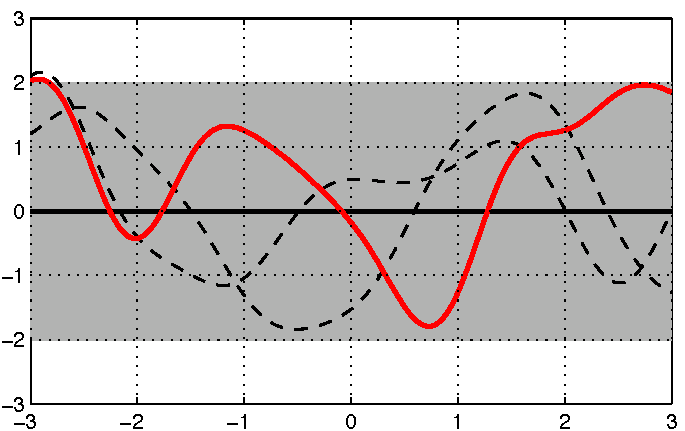
\includegraphics[scale=0.67, clip, trim = 0.5cm 0.45cm 0.2cm 0cm]{figs/gpml/priorGP.pdf}};
	\node at (3.3,-2) {$\bz$};
	\node at (-3.05,1.75) {$\bff(\bz)$};
\end{tikzpicture}
}
\hfill
\subfigure[Samples from the GP posterior $p(\bff|\cD,\hyp)$.]{
\tikzstyle{line} = [draw, -latex]
\begin{tikzpicture}
	\node at (0,0) {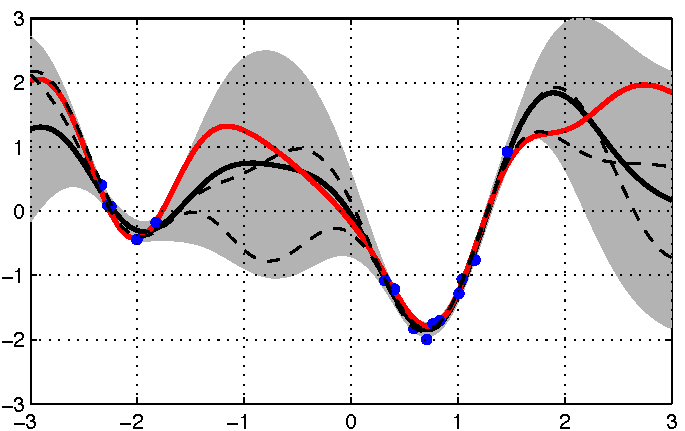
\includegraphics[scale=0.67, clip, trim = 0.5cm 0.45cm 0.2cm 0cm]{figs/gpml/postGP.pdf}};
	\node at (3.3,-2) {$\bz$};
	\node at (-3.05,1.75) {$\bff(\bz)$};
\end{tikzpicture}
\label{fig:post}
}
\caption{Samples from a Gaussian process prior and posterior after data from the underlying function has been observed. The red, black and dashed lines show the underlying function $\bff$, mean of the Gaussian process (prior $\bmm$ and posterior $\bmm_+$) and sampled functions respectively. The grey regions denote two standard deviations, or 95\% confidence region, of the GP distribution. Training data is shown as blue dots on the posterior plot.}
\label{fig:priorpost}
\end{figure}
%-------------------------------------------------------------------------------------------------------------------------------------------


\subsubsection{Posterior}
Given the observed training data set $\cD$ it is desirable to update this prior and form a posterior distribution over the space of functions. This posterior distribution is related to the prior and the training data through Bayes' rule
\begin{equation}
p(\bff|\cD,\hyp) = \frac{p(\bY|\bff,\bZ,\hyp)}{p(\bY|\bZ,\hyp)} p(\bff|\hyp)
\label{eqn:gpbayes}
\end{equation}
with likelihood $p(\bY|\bff,\bZ,\hyp)$ and prior $p(\bff|\hyp)=p(\bff|\bZ,\hyp)$ which is independent of the training inputs. The marginal likelihood term is given by the following equivalent integrals
\begin{align}
p(\bY|\bZ,\hyp) &= \int p(\bY|\bff,\bZ,\hyp)p(\bff|\hyp)\dd\bff 
= \int p(\bY|\bF,\hyp)p(\bF|\bZ,\hyp)\dd\vec\bF
\label{eqn:marlik}
\end{align}
These expressions are equivalent because the observed data set $\bY$ is related to the underlying function $\bff$ only through the underlying values $\bF$ since the likelihood has no notion of the prior beliefs. We shall discuss the importance of this term for training the hyperparameters of a Gaussian process in the following section. Note that the dependence on the structure $\cH$ is assumed implicitly through the hyperparameters. It turns out that this posterior distribution over functions is also a Gaussian process and can be calculated analytically as demonstrated in \Theo{GPpost}. This is again a standard result from the Machine Learning community.






\begin{theo}[Gaussian Process Posterior] \label{theo:GPpost}
Assume that the function $\bff$ has been drawn from some Gaussian process prior $\bff|\hyp \sim \mathcal{GP}(\bO,\bK)$ with hyperparameters $\hyp$ and that the data set $\cD$ given by \Eq{cZY} has been observed. The posterior distribution is also a Gaussian process $\bff|\cD,\hyp \sim \mathcal{GP}(\bmm_+,\bK_+)$ with mean and covariance function
\begin{align}
\bmm_{+}(\bz) &= \bK(\bz,\bZ) \big(\bK_{nn}+\bS_{\be}\otimes\bI\big)^{-1} \vec\bY  \label{eqn:gpmean} \\
\bK_{+}(\bz,\tilde\bz) &= \bK(\bz,\tilde\bz) - 
\bK(\bz,\bZ) \big(\bK_{nn}+\bS_{\be}\otimes\bI\big)^{-1}\bK(\bZ,\tilde\bz) \label{eqn:gpvar}
\end{align}
\espa
\end{theo}

\begin{proof}
Consider the joint distribution of the noisy observed states $\bY$ and the function values $\bff(\bz)$ and $\bff(\tilde\bz)$ to be inferred
\begin{equation}
\left.\bmat{\vec\bY \\ \bff(\bz) \\ \bff(\tilde\bz)} \right| \bz, \tilde\bz, \bZ, \hyp  \sim \cN\left(
\bO,
\bmat{\bK_{nn}+\bS_{\be}\otimes\bI & \bK(\bZ,\bz) & \bK(\bZ,\tilde\bz) \\ 
\bK(\bz,\bZ) & \bK(\bz,\bz) & \bK(\bz,\tilde\bz) \\
\bK(\tilde\bz,\bZ) & \bK(\tilde\bz,\bz) & \bK(\tilde\bz,\tilde\bz)}
\right)
\end{equation}
By conditioning on the observed outputs $\bY$ using the identity for a Gaussian conditional distribution, from \App{gauss}, the result follows.
\qed
\end{proof}

It is clear that this predictive form is exactly the same as was obtained in \Eqs{rbfM2}{rbfV2} by following a parametric approach and extending to possibly infinite dimensional feature spaces using the kernel trick. However in this case the covariance function has been defined directly and there is no need to appeal to a parametric interpretation in terms of a feature vector or a finite set of basis functions.
%
Note that if the covariance function is in the form of a radial basis function, the predictive mean is in the form of a linear sum radial basis functions each centred on a training data point $\bmm_{+}(\bz) = \bK(\bz,\bZ) \bBe$ where $\bBe = \big(\bK_{nn}+\bS_{\be}\otimes\bI\big)^{-1} \vec\bY$.

The process of choosing a prior distribution over function space and forming the posterior based on training data is shown in \Fig{priorpost}. The posterior shown in \Fig{post} clearly shows that in regions where there is a lot of training data the uncertainty in functional predictions reduces significantly whereas in regions with little training data the distribution collapses back to the prior.
Therefore, given an arbitrary state-action pair $\bz_k$, training data set $\cD$ and Gaussian process prior over function space, the predictive distribution over the next state $p(\bx_{k+1}|\bz_k,\cD)$ can be obtained analytically. 








%It is interesting to note that Eq.~(\ref{gpmean}) is in the form of a nominal function of the inputs plus a linear sum of basis functions defined by the covariance function each centred on a point in the training data set
%\begin{align}
%\bm_{\Delta}(\bz_*) &= \bmm(\bz_*) + \bK(\bz_*,\bZ) \bBe
%\end{align}
%where $\bBe = \bK_{\be}^{-1} \big(\vec\bY - \bmm(\bZ)\big) \in \RR^{nE}$ is simply a weighting vector. 


\subsection{Model Selection and Training} \label{sec:nLML}
The preceding section laid out the framework for prediction using a Gaussian process prior with known structural form $\cH$ and hyperparameters $\hyp$. In practice, the form and parameters governing the prior are unknown, and are in fact a construct that has been created in order to view the inference problem from a Bayesian perspective. A fully Bayesian approach to addressing the model selection problem, as outlined in \cite{RaWi06} Chapter 5, can be viewed through the hierarchy depicted by the graphical model in \Fig{modsel}. In this framework a distribution is maintained over hyperparameters and possible model structures as well as the function space itself.

In this thesis, we shall not adopt the fully Bayesian treatment of model selection due to the analytic intractability of integrating over hyperparameter distributions and computational complexity of approximating it using sampling methods. We will assume that the model structure $\cH$ has been chosen beforehand based on intuition about the problem at hand and that a point estimate of the hyperparameters $\hat\hyp$ is chosen based on an evidence maximisation scheme which will now be motivated.

%-------------------------------------------------------------------------------------------------------------------------------------------
\begin{figure}[t]
\centering
%
\tikzstyle{sum} = [circle, draw, minimum height=.8cm]
\tikzstyle{line} = [draw, -latex]
\begin{tikzpicture}
	\node[sum] (H) at (0,2.25) {$\cH$}; \node[sum] (h) at (0,0.75) {$\hyp$};
	\node[sum] (w) at (0,-0.75) {$\bff$}; \node[sum, fill=black!30] (D) at (0,-2.25) {$\cD$};
	\path[line] (H) -- (h); \path[line] (h) -- (w); \path[line] (w) -- (D);
	\node[] at (2.5,2.25) {\small \textit{level 3:} model structure};
	\node[] at (2.6,0.75) {\small \textit{level 2:} hyperparameters};
	\node[] at (2,-0.75) {\small \textit{level 1:} function};
	\node[] at (1.1,-2.25) {\small data};
\end{tikzpicture}
%
\caption{Graphical model depicting the model selection hierarchy from possible model structures $\cH$ to the associated hyperparameters $\hyp$ which in turn control the distribution over the actual underlying function $\bff$ which determines the observed data set $\cD$. The clear nodes depict hidden variables and the gray nodes depict observed variables.}
\label{fig:modsel}
\end{figure}
%-------------------------------------------------------------------------------------------------------------------------------------------

Level 1 inference was discussed in the previous section and is concerned with determining the posterior over function space $p(\bff|\cD,\hyp)$ once a training data set had been observed and given some known hyperparameters. This was achieved using Bayes' rule in \Eq{gpbayes} and it turned out that this could be found analytically in the form of \Eqs{gpmean}{gpvar}.

Level 2 inference considers the distribution over hyperparameters $\hyp$ given a specific model structure $\cH$. The posterior after observing a training data set is again given by Bayes' rule as
\begin{equation}
p(\hyp|\cD) = \frac{p(\bY|\bZ,\hyp)}{p(\bY|\bZ)} p(\hyp) \label{eqn:hypbayes}
\end{equation}
Again, dependence of each term on the model structure is taken implicitly. Now a sensible point estimate for the hyperparameters would be the Maximum A Posteriori (MAP) estimate $\hat\hyp \in \arg\!\max_{\hyp}p(\hyp|\cD)$. Taking a flat prior over hyperparameters means that $p(\hyp|\cD) \propto p(\bY|\bZ,\hyp)$. Therefore maximising the marginal likelihood (or log-marginal likelihood) from \Eq{gpbayes} is equivalent to the MAP estimate of the hyperparameters. This can be written analytically as
\begin{align}
-\log p(\bY|\bZ,\hyp) = 
\underbrace{ \tfrac{1}{2} \big(\vec\bY-\bmm(\bZ)\big)\T \bK_{\be}^{-1} \big(\vec\bY-\bmm(\bZ)\big) }_
{\text{data fit}}
+ \underbrace{\tfrac{1}{2}\log\big|\bK_{\be}\big|}_
{\text{complexity}} + \tfrac{En}{2}\log 2\pi \label{eqn:logmar}
\end{align}
where $\bz \in \RR^D$, $\bK_{\be} = \bK_{nn}+\bS_{\be}\otimes\bI$ since the likelihood $p(\bY|\bF,\bZ,\hyp) = \cN(\vec\bF,\bS_{\be}\otimes\bI)$ and prior $p(\bF|\bZ,\hyp) = \cN\big(\bmm(\bZ), \bK_{nn}\big)$ are simply multivariate Gaussians.

As highlighted in Chapter 5.4 of \cite{RaWi06}, maximising the marginal likelihood leads to some intuitive properties in terms of the trade off between data fit and model complexity. In non-rigorous terms we consider the complexity of a given model to be how quickly the function varies as we move around the $\bz$ space. If the function changes very rapidly then data observed in one region of the $\bz$ space will only be useful for making predictions very close to that region (an exception to this would be if we considered periodic covariance functions). Conversely, if the variations are slow then data observed in one region of the space may be generalised to make predictions in the surrounding regions. 

We shall now provide a crude argument for why the log likelihood in \Eq{logmar} trades off data fit with complexity. Consider a zero mean prior with squared exponential covariance term. As the length scales are increased, the terms in $\bK_{\be}$ become more correlated and therefore the complexity term $\big|\bK_{\be}\big|$ decreases. However at the same time the ``size" of the inverse $\bK_{\be}\inv$ increases and therefore deviations from the prior mean are penalised more heavily. If we maximise the marginal likelihood, we are looking for \textit{the least complex model that explains the data.}





\subsection{Sparse Approximations} \label{sec:sparse}
One of the greatest problems in employing a full Gaussian process model is the computational requirements required as the data set increases. The source of this burden lies mainly in the inversion of the kernel matrix $\bK_{nn}$ and its multiplication with vectors. This issue can be addressed by finding low-rank approximations to this matrix and most of these methods can be viewed under the unifying framework of \cite{QR05}. In this thesis we shall consider the Fully Independent Training Conditional (FITC) approximation (or sparse Gaussian processes using pseudo-inputs) defined by \cite{SG06}. We find this to be a more elegant approach than simply throwing away a subset of the data points.

The FITC approximation assumes that a fictitious (or pseudo) data set $\cD_{\text{p}} = \{\bZ_{\text{p}},\bF_{\text{p}}\}$ of $m<n$ data points is available alongside the actual data $\cD$. Note that it would be meaningless to introduce noise onto the pseudo-targets $\bF_{\text{p}}$ and use $\bY_{\text{p}}$ instead. It turns out that we do not actually need to define values for $\bF_{\text{p}}$ since their effect can be integrated out analytically
\begin{align*}
p(\bY | \bZ, \bZ_{\text{p}}) &= \int p(\bY | \bZ, \bZ_{\text{p}}, \bF_{\text{p}}) p(\bF_{\text{p}} | \bZ_{\text{p}}) \dd \vec{\bF}_{\text{p}} \\
&= \int \cN\big(\vec\bY | \bK_{nm}\bK_{mm}\inv\vec{\bF}_{\text{p}}, \bGam\big) 
\cN\big(\vec{\bF}_{\text{p}} | \bO, \bK_{mm}\big) \dd \vec{\bF}_{\text{p}} \\
&= \cN\big( \vec\bY| \bO, \bQ_{nn} + \bGam \big)
\end{align*}
where $\bK_{nm} := \bK(\bZ,\bZ_{\text{p}})$, $\bK_{mm} := \bK(\bZ_{\text{p}},\bZ_{\text{p}})$ and $\bQ_{nn} := \bK_{nm}\bK_{mm}\inv\bK_{mn}$ is clearly a low rank approximation of $\bK_{nn}$. The matrix $\bGam$ is specific to the FITC approximation and is defined as
\begin{equation*}
\bGam := \diag\{\bK_{nn} - \bQ_{nn}\} + \bS_{\be} \otimes \bI
\end{equation*}
which is distinct from many of the other sparse approximate methods which simply use $\bGam = \bS_{\be} \otimes \bI$. When training, the locations of these pseudo-inputs $\bZ_{\text{p}}$ are optimised along with the hyperparameters $\hyp$.

Now to determine the Gaussian process posterior prediction under this approximation. The posterior mean and covariance are now defined as
\begin{align}
\bmm_{+}(\bz) &= \bK(\bz,\bZ_{\text{p}}) \bB\inv \bK_{mn} \bGam\inv \vec\bY \\
%
\bK_{+}(\bz,\tilde\bz) &= \bK(\bz,\tilde\bz) - \bK(\bz,\bZ_{\text{p}}) \big(\bK_{mm}\inv - \bB\inv\big)\bK(\bZ_{\text{p}},\tilde\bz)
\end{align}
where $\bB := \bK_{mm} + \bK_{mn}\bGam\inv\bK_{nm}$. It is important to note that these equations are in exactly the same form as \Eqs{gpmean}{gpvar} with respect to the test inputs $\bz$ and $\tbz$. This means that employing the FITC sparse approximation will have no effect on our discussion of multiple-step ahead predictions in \Sec{multistep}.





\subsection{Priors for General Nonlinear Functions} \label{sec:kernels}
\subsubsection{Squared Exponential Kernel}

Attention shall now be given to a particular choice of kernel $\bK$, the Squared Exponential (SE). 
To motivate the use of this kernel, consider the single state case where $E=1$. The analysis in the section closely follows that given by \cite{Dei09} in Section 2.2. The standard form of the SE kernel is
\begin{equation}
k_{\text{SE}}(\bz,\tilde\bz) = \alpha^2 \exp\Big(-\tfrac{1}{2}(\bz - \tilde\bz)\T\bLa^{-1}(\bz - \tilde\bz) \Big)
\label{eqn:SEkernel}
\end{equation}
with hyperparameters $\hyp \in \RR^{D+1}$ consisting of an output variance $\alpha^2$ and a diagonal matrix of input length-scales $\bLa = \diag\big\{[\lambda_1^2 \dots \lambda_D^2]\big\}$. \Theo{SEkernel} shows that this kernel defines a prior distribution over the space of all functions in the class of a given universal function approximator.

\begin{theo}[Squared Exponential Kernel] \label{theo:SEkernel}
Consider the function $f:\RR^D \rightarrow \RR$ parameterised by a universal function approximator of the form
\begin{equation}
f(\bz) = \int_{\RR^D}  \phi(\bz,\bs) \gamma(\bs) \dd\bs 
= \int_{\RR^D}  \exp\left( -(\bz-\bs)\T\bLa^{-1}(\bz-\bs) \right)  \gamma(\bs)  \dd\bs
\label{eqn:universalapp}
\end{equation}
where $\gamma(\bs)$ is a weighting function. Assuming a normal Gaussian prior over the weights $\gamma(\bs) \sim \cN(0,1)$ is equivalent to assuming $f \sim \mathcal{GP}(0,k_{\text{SE}})$ has been drawn from a Gaussian process with zero mean and squared exponential covariance function given in \Eq{SEkernel}.
\spa \end{theo}

\begin{proof}
The equivalent Gaussian process representation of this problem will have a mean function given by $\EE_{\gamma}[f(\bz)]$ and covariance function given by $\cov_{\gamma}[f(\bz),f(\tilde\bz)] $. The mean is calculated as
\begin{align*}
\EE_{\gamma}[f(\bz)] &= \int f(\bz) p\big(\gamma(\bs)\big) \dd\gamma(\bs) 
= \int \phi(\bz,\bs) \bigg( \int \gamma(\bs) p\big(\gamma(\bs)\big) \dd\gamma(\bs) \bigg) \dd\bs = 0
\end{align*}
since $\EE_{\gamma}[\gamma(\bs)] = 0$. Now, because the prior mean function equals zero the prior covariance is
\begin{align*}
\cov_{\gamma}[f(\bz),f(\tilde\bz)] &= \EE_{\gamma}[f(\bz)f(\tilde\bz)] \\
&= \int f(\bz) f(\tilde\bz) p\big(\gamma(\bs)\big) \dd\gamma(\bs) \\
&= \int \phi(\bz,\bs) \phi(\tilde\bz,\bs) \bigg( \int \gamma(\bs)^2 p\big(\gamma(\bs)\big) \dd\gamma(\bs) \bigg) \dd\bs \\
&= \int \phi(\bz,\bs) \phi(\tilde\bz,\bs) \dd\bs
\end{align*}
since $\EE_{\gamma}[\gamma(\bs)^2] = 1$. Now because $\phi$ produces an unnormalised Gaussian this integral is tractable and from \Eq{universalapp}
\begin{equation*}
\cov_{\gamma}[f(\bz),f(\tilde\bz)] = \alpha^2 \exp\Big(-\tfrac{1}{2}(\bz - \tilde\bz)\T\bLa^{-1}(\bz - \tilde\bz) \Big)
\end{equation*}
for a suitable $\alpha$. This is exactly the form of the SE kernel in \Eq{SEkernel}.
\qed
\end{proof}

Informally, the SE covariance function provides a means of placing a prior over the space of all smooth, or infinitely differentiable functions, with intrinsic input length scales. 




\subsubsection{Additive Squared Exponential Kernel} 
A related class of kernel functions is the additive squared exponential family. These are useful in the situation where we wish to parameterise a distribution over a space of additively separable functions. The family of first-order additive functions are as follows
\begin{align*}
\bff(\bz) &= \sum_{i=1}^D  \bff_i\big(z[i]\big)
\end{align*}
We may also wish to consider higher order interaction terms.
We shall consider a general additive form in which the orders of interaction are stored in the set $\cI$ and can be written mathematically as
\begin{align}
\bff(\bz) &= \sum_{\bi \in \cI}  \bff_\bi\big(\bz[\bi]\big)
\end{align}
For example if we know our function is an additive combination of nonlinear functions with respect to the first, third and a combination of the second and third components of the state-action space then $\cI = \{1,3,[2;3]\}$. Considering $D\tth$ order interactions $\cI = \{[1 \dots D]\}$ will obviously brings us back to the completely general function $\bff(\bz)$. 
%
Now a kernel that parameterises a prior distribution over such a space is the additive squared exponential which we define as follows
\begin{equation}
k_{\text{aSE}}(\bz,\tilde\bz) = \sum_{\bi \in \cI} \alpha_{\bi}^2 \exp\Big(-\tfrac{1}{2}\big(\bz[\bi] - \tilde\bz[\bi]\big)\T\bLa_{\bi}^{-1}\big(\bz[\bi] - \tilde\bz[\bi]\big) \Big)
\label{eqn:aSEkernel}
\end{equation}
where it is clear that setting $\cI = \{[1 \dots D]\T\}$ recovers the standard squared exponential kernel.

In the literature the first order additive structure appears under Generalized Additive Models (GAMs) as introduced by \cite{HT90}. The general kernel involving all possible interactions was recently introduced by \cite{DNR11}. The authors attack the main drawback this general kernel, which is the computational effort required to calculate all the terms, which scales as $\cO(2^n)$. They present a neat iterative method of evaluating all the additive kernels in $\cO(D^2)$ making it a useful and computationally tractable model to work with. This method requires that the $\alpha_{\bi}$ and $\bLa_\bi$ parameters are common for each order of interaction, which is not too restrictive. It is based on the Newton-Girard formulae, which assumes that the function can be decomposed as a product
\begin{equation*}
k_{\text{aSE}}(\bz,\tilde\bz) = \sum_{\bi \in \cI} \alpha_{\bi}^2 \prod_{i\in \bi} \exp\Big(-\tfrac{1}{2}\big(z[i] - \tilde z[i]\big)^2/\lambda_{i}^{2} \Big)
\end{equation*}
As we shall see in \Sec{multistep} this decomposable structure is lost when we are considering prediction at an uncertain state-input and therefore this iterative method cannot be used. Therefore for most applications we will only be considering separating first order, and maybe second order, interactions and leaving higher order ones to be explained by a standard SE kernel.







\section{Multiple-Step Predictions} \label{sec:multistep}
\subsection{Overview}
A framework for maintaining a Gaussian distribution over whole trajectories $\btau$ based on a moment matching approximation was outlined in \Sec{xuprediction}. In order for a Gaussian process model to fit into this framework the mean $\bmm$ and covariance function $\bK$ must be of a form such that the expectation $\bm_* = \EE_{\bz,\bff}[\bff(\bz)]$ and covariance $\bS_* = \cov_{\bz,\bff}[\bff(\bz)]$ are analytically tractable given $\bff\sim\mathcal{GP}(\bmm_+,\bK_+)$ and $\bz \sim \cN(\bm,\bS)$. The posterior mean $\bmm_+$ and covariance $\bK_+$ are related to the input mean $\bm$ and covariance $\bS$ through the GP predictive equations given in \Eqs{gpmean}{gpvar}. Through separation of the integrals with respect to the random function $\bff$ and the input $\bz$ the expectation, covariance and output-input covariance can be broken down as follows
\begin{align}
\bm_* &=  \EE_{\bz,\bff}[\bff(\bz)]
&& \!\!\!\!\!\!\!\!\!\!\!\!\!\!\!\!\!\!\!\!\!\!\!\!\!\!\!\!\!\!\!\!\!\!\!\!\!\!\!\!\!\!\!\!\!\!\!\!\!
= \EE_{\bz}[\bmm_+(\bz)] \label{eqn:uncM} \\
\bS_* &= \cov_{\bz,\bff}[\bff(\bz)] 
&& \!\!\!\!\!\!\!\!\!\!\!\!\!\!\!\!\!\!\!\!\!\!\!\!\!\!\!\!\!\!\!\!\!\!\!\!\!\!\!\!\!\!\!\!\!\!\!\!\!
= \EE_{\bz}\big[\bK_+(\bz) + \bmm_+(\bz)\bmm_+(\bz)\T\big] - \bm_*\bm_*\T \label{eqn:uncV} 
\end{align}
An example of the moment matching approximation for the posterior GP shown in \Fig{post} is given in \Fig{multiprop}. The exact expressions for these equations shall now be derived for a linear mean function along with a linear, squared exponential or additive squared exponential covariance function.







%-------------------------------------------------------------------------------------------------------------------------------------------
\begin{figure}[t]
\centering
\small
\tikzstyle{line} = [draw, -latex]
\begin{tikzpicture}
\node at (0,-3) {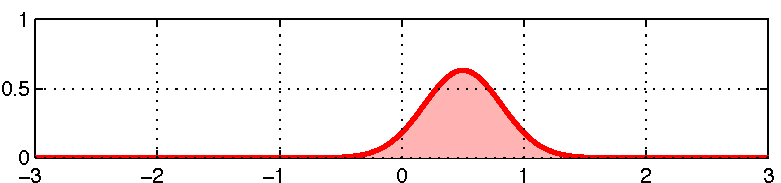
\includegraphics[scale=0.6, clip, trim=0.5cm 0.3cm 0cm 0cm]{figs/gpml/propGP_1.pdf}};
\node at (0.025,0) {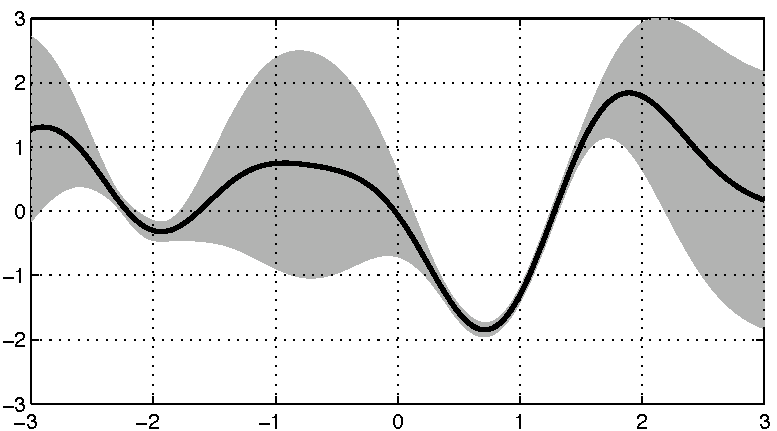
\includegraphics[scale=0.6, clip, trim=0.5cm 0.4cm 0cm 0cm]{figs/gpml/propGP_2.pdf}};
\node at (4.7,0) {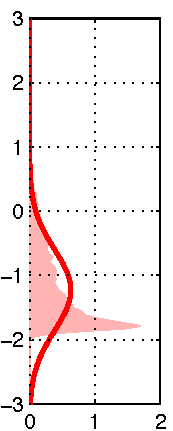
\includegraphics[scale=0.6, clip, trim=0.45cm 0.4cm 0cm 0cm]{figs/gpml/propGP_3.pdf}};

\node[rotate=90] at (-4.13,0) {Gaussian process};
\node[rotate=-90] at (5.65,0) {\color{red}Output distribution};
\node at (0,-4.1) {\color{red}Input distribution};

\node at (-3.1,1.55) {$p(\bff)$};
\node at (-3.1,-2.7) {\color{red}$p(\bz)$};
\node at (4.7,1.55) {\color{red}$p\big(\bff(\bz)\big)$};

\end{tikzpicture}
\caption{The moment matching approximation for a Gaussian process evaluated at a distribution over state-actions $p(\bz)$. The red lines depict the Gaussian approximations to the true distributions given by the red shaded areas.}
\label{fig:multiprop}
\end{figure}
%-------------------------------------------------------------------------------------------------------------------------------------------





\subsection{Parametric Form}
\subsubsection{General Basis Functions}
We shall first consider the predictive equations $\bmm_+(\bz)$ and $\bK_+(\bz)$ for a parametric model consisting of a linear sum of known basis functions as given in \Eqs{rbfM}{rbfV}. Remember that this approach can be viewed from a function space perspective as a Gaussian process for which there exists a finite inner product representation of the covariance function $\bK(\bz,\tilde\bz) = \bPh(\bz)\T\bOm\bPh(\tilde\bz)$. 
%
The elements of the terms in \Eqs{uncM}{uncV} are given by 
\begin{align*}
\mu_{*}[i] &= 
\EE_{\bz}\big[\bph_{i}\big]\T \bet_{+} \\
%
\Sigma_{*}[i,j] &= 
\tr\Big(\EE_{\bz}\big[\bph_{i}\bph_{j}\T\big] \big(\bOm_{+}+\bet_+\bet_+\T\big) \Big) 
- \mu_{*}[i]\mu_{*}[j]
\end{align*}
for $i,j \in \ZZ_{[1,E]}$ where $\bph_{i} = \Phi[:,i](\bz)$. 
%
With the use of the Kronecker and Hadammard products we can actually define an expression for the full mean $\bm_*$ and covariance $\bS_*$ as follows
\begin{align}
\bm_* &= (\bI_E \otimes \mathbf{1}_P\T) \Big( \EE_{\bz}\big[\vec{\bPh}\big] \circ \big(\mathbf{1}_E \otimes \bet \big) \Big)
 \label{eqn:uncparamM}  \\
%
\bS_* &= 
 (\bI_E \otimes \mathbf{1}_P\T)
\Big( \EE_{\bz}\big[\vec{\bPh}\vec{\bPh}\T\big]  \circ 
\big(\mathbf{1}_{E\times E} \otimes (\bOm+\bet\bet\T) \big) \Big) 
 (\bI_E \otimes \mathbf{1}_P)
- \bm_*\bm_*\T
\label{eqn:uncparamV}
\end{align}
where $\vec{\bPh} = \vect\big(\bPh(\bz)\big)$. Note that the $(\bI_E \otimes \mathbf{1}_P)$ terms act as a kind of multivariable trace operator in the expression for $\bS_*$. We could not find this form anywhere in the literature and therefore the derivation of it is our own.
%
This expression means that the only requirement on the feature matrix is that the expectations $\EE_{\bz}\big[\vec{\bPh}]$ and $\EE_{\bz}\big[\vec{\bPh}\vec{\bPh}\T\big]$ can be evaluated analytically.





\subsubsection{Linear Model}
For the standard linear model the feature matrix is given by $\bPh(\bz) = \bI \otimes \bz$, \Eqs{uncparamM}{uncparamV} take the following simplified form
\begin{align}
\bm_* &= (\bI_E \otimes \mathbf{1}_D\T) \Big( \big( \mathbf{1}_E \otimes \EE_{\bz}[\bz] \big) \circ \bet \Big) 
\label{eqn:linMU} \\
%
\bS_* &= 
 (\bI_E \otimes \mathbf{1}_D\T)
\Big( \big(\mathbf{1}_{E\times E} \otimes \EE_{\bz}\big[\bz\bz\T\big] \big) \circ 
 \big(\bOm+\bet\bet\T\big) \Big) 
 (\bI_E \otimes \mathbf{1}_D)
- \bm_*\bm_*\T
\label{eqn:linSIG}
\end{align}








\subsection{Nonparametric Form}

\subsubsection{General Covariance Function}
We now turn our attention back to the more general nonparametric form of these equations. Consider the standard Gaussian process predictive equations given in \Eqs{gpmean}{gpvar}. The elements of the predictive equations in \Eqs{uncM}{uncV} are given by 
%%
\begin{align*}
\mu_*[i] &= 
\EE_{\bz}\big[\bk_{i}\big]\T \bBe \\
%
\Sigma_*[i,j] &= 
\EE_{\bz}\big[k_{ij}\big] + \tr\Big(\EE_{\bz}\big[\bk_{i}\bk_{j}\T\big]
\big(\bK_{\be}^{-1} + \bBe\bBe\T\big) \Big) 
- \mu^{(i)}_* \mu^{(j)}_*
\end{align*}
%%
for $i,j \in \ZZ_{[1,E]}$ where $\bk_{i} = K[:,i](\bZ,\bz)$ is the $i\tth$ column of $\bK(\bZ,\bz)$ and $k_{ij}=K[i,j](\bz)$ is the $(i,j)\tth$ element of $\bK(\bz)$. 
Note that if we are employing a sparse GP approximation then we simply replace the vector $\bBe$ and matrix $\bK_{\be}$ with the appropriate terms and the rest of the analysis remains the same.
Now, as with the parametric form, expressions may be written for the full mean and covariance as follows
%%
\begin{align}
\bm_* &= (\bI_E \otimes \mathbf{1}_n\T)
\Big( \EE_{\bz}\big[\vec{\bK}\big] \circ \big(\mathbf{1}_E \otimes \bBe \big) \Big)
 \label{eqn:uncgpM}  \\
%
\bS_* &= 
\EE_\bz[\bK(\bz)] + 
 (\bI_E \otimes \mathbf{1}_n\T)
\Big( \EE_{\bz}\big[\vec{\bK}\vec{\bK}\T\big]  \circ 
\big(\mathbf{1}_{E\times E} \otimes (\bK_{\be}^{-1} + \bBe\bBe\T) \big) \Big) 
 (\bI_E \otimes \mathbf{1}_P)
- \bm_*\bm_*\T
\label{eqn:uncgpV}
\end{align}
%%
where $\vec{\bK} = \vect\big( \bK(\bZ,\bz) \big)$. Again, this is a novel parameterisation that has not been found in the literature.
%
Similarly to the parametric form, the only requirements on the covariance function is that the expectations $\EE_{\bz}\big[\bK(\bz)\big]$, $\EE_{\bz}\big[\vec{\bK}\big]$ and $\EE_{\bz}\big[\vec{\bK}\vec{\bK}\T\big]$ are analytically tractable. In most cases, stationary covariance functions will be considered i.e.\ $\bK(\bz,\tilde\bz) = \bK(\bz-\tilde\bz)$ therefore $\bK(\bz)$ will be a constant matrix. The remaining expectations will be made up of the building blocks
\begin{align}
\EE_{\bz}\big[ k_a(\ba,\bz) \big] \quad \text{and} \quad
\EE_{\bz}\big[ k_a(\ba,\bz)k_b(\bb,\bz) \big] \label{eqn:exps}
\end{align}
where $k_a(\ba,\bz)$ and $k_b(\bb,\bz)$ are elements of $\bK(\ba,\bz)$ and $\bK(\bb,\bz)$ respectively and $\ba,\bb \in \bZ$. We will now evaluate these expectations for the squared exponential kernel.







\subsubsection{Squared-Exponential Kernel} 
The following derivations can be found in \cite{Dei09}, Section 2.3 or \cite{GRQM03} for the univariate case. Consider the squared exponential kernel defined in \Eq{SEkernel}. The first expectation in \Eq{exps} can then be expanded as
\begin{align}
\nonumber \EE_{\bz}\big[ k_a(\ba,\bz) \big] 
&= \int k_a(\ba,\bz) \cN(\bz|\bm,\bS) \dd\bz \\
\nonumber &= \alpha_a^2(2\pi)^{\sfrac{D}{2}} |\bLa_a|^{\sha}  \int  \cN(\bz|\ba,\bLa_a) \cN(\bz|\bm,\bS)  \dd\bz   \\[-0.3cm]
\nonumber &= \alpha_a^2 (2\pi)^{\sfrac{D}{2}} |\bLa_a|^{\sha} \cN\big(\bm|\ba,\bLa_a+\bS\big) 
\overbrace{ \int \cN\big(\bz|\bm_{\ba},\bS_{\ba} \big)  \dd\bz }^{ 1 }   \\
&=  \alpha_a^2  \big|\bS\bLa_a\inv + \bI\big|^{-\sha} \exp\Big( -\half(\ba-\bm)\T(\bLa_a+\bS)\inv (\ba-\bm)\Big) 
\label{eqn:SEpropM}
\end{align}
The first step is made by pulling out the normalising constant for the squared exponential kernel to make it a Gaussian and the second step is due to the identity for the multiplication of two Gaussian densities given in \App{gauss}. Note that setting $\bS = \sigma\bI$ and letting $\sigma \rightarrow 0$, the standard expression for the SE kernel is recovered as expected. The mean $\bm_{\ba}$ and covariance $\bS_{\ba}$ are given by
\begin{align}
\bm_{\ba} &:= (\bLa_a\inv + \bS\inv)\inv \big(\bLa_a\inv\ba + \bS\inv\bm \big)
&&\!\!\!\!\!\!\!\!\!\!\!\!\!\!\!\!\!\!\!\!\!\!\!\!\!\!\!\!\!\!\!\!\!=  (\bS\bLa_a\inv + \bI)\inv \big( \bS\bLa_a\inv\ba + \bm \big)
\label{eqn:muA} \\
\bS_{\ba} &:= (\bLa_a\inv + \bS\inv)\inv
&&\!\!\!\!\!\!\!\!\!\!\!\!\!\!\!\!\!\!\!\!\!\!\!\!\!\!\!\!\!\!\!\!\!= (\bS\bLa_a\inv + \bI)\inv \bS
\label{eqn:sigA}
\end{align}
which can be written in a form in which there is no need to invert the potentially singular matrix $\bS$ explicitly.
Now turning to the second expectation in \Eq{exps} and following a similar procedure gives
\begin{align*}
\EE_{\bz}[k_a(\ba,\bz)&k_b(\bb,\bz)\big] \\
&= \int k_a(\ba,\bz)k_b(\bb,\bz) \cN(\bz|\bm, \bS) \dd\bz \\
%
&= \alpha_a^2\alpha_b^2 (2\pi)^{D} |\bLa_a|^{\sha} |\bLa_b|^{\sha}
\int \cN(\bz|\ba,\bLa_a)\cN(\bz|\bb,\bLa_b) \cN(\bz|\bm, \bS) \dd\bz  \\[-0.3cm]
%
&= \alpha_a^2\alpha_b^2 (2\pi)^{D} |\bLa_a|^{\sha} |\bLa_b|^{\sha}
\cN\big(\ba|\bb,\bLa_a+\bLa_b\big) \cN\big(\bm|\hat\bm,\hat\bS \big)
\overbrace{ \int \cN(\bz|\bm_{\ba\bb},\bS_{\ba\bb}) \dd\bz }^{ 1 } \\
%
&= \alpha_a^2 \alpha_b^2 \big|\bS(\bLa_a\inv + \bLa_b\inv) + \bI\big|^{-\sha}
\exp\Big( -\half(\ba-\bb)\T(\bLa_a + \bLa_b)\inv (\ba-\bb) \Big) \\
&\quad\quad\quad\quad\quad\quad\quad\quad\quad\quad\quad\quad\quad\quad\quad\quad\quad\quad
 \exp\Big( -\half(\hat\bm-\bm)\T(\hat\bS + \bS)\inv (\hat\bm-\bm) \Big)
\end{align*}
where $\hat\bm := \hat\bS(\bLa_a\inv\ba + \bLa_b\inv\bb)$ and $\hat\bS := (\bLa_a\inv + \bLa_b\inv)\inv$. This can be written in a more intuitive manner by expanding and collecting terms in the exponents
%
\begin{equation}
\EE_{\bz}[k_a(\ba,\bz)k_b(\bb,\bz)\big] = k_a(\ba,\bm)k_b(\bb,\bm) \big|\bR\big|^{-\sha}
\exp\Big( \half\bar\bm\T \bR\inv\bS \bar\bm \Big)
\label{eqn:SEpropV}
\end{equation}
%
where $\bR := \bS(\bLa_a\inv+\bLa_b\inv) + \bI$ and $\bar\bm := \bLa_a\inv(\ba-\bm) + \bLa_b\inv(\bb-\bm)$. Note that $\bR\inv\bS = (\bLa_a\inv+\bLa_b\inv + \bS\inv)\inv$ is a symmetric matrix and can again be computed without explicit inversion of $\bS$. For completeness, note that the mean $\bm_{\ba\bb}$ and covariance $\bS_{\ba\bb}$ are given by
\begin{align}
\bm_{\ba\bb} &:= (\bLa_a\inv + \bLa_b\inv + \bS\inv)\inv \big(\bLa_a\inv\ba + \bLa_b\inv\bb + \bS\inv\bm \big)
&&\!\!\!\!\!\!=  \bR\inv \big( \bS(\bLa_a\inv\ba + \bLa_b\inv\bb) + \bm \big)
\label{eqn:muAB} \\
\bS_{\ba\bb} &:= (\bLa_a\inv + \bLa_b\inv + \bS\inv)\inv
&&\!\!\!\!\!\!= \bR\inv \bS
\label{eqn:sigAB}
\end{align}
To conclude, the expectations required for moment matching in \Eq{exps} are given by \Eqs{SEpropM}{SEpropV} for the squared exponential kernel defined in \Eq{SEkernel}.



\subsubsection{Additive Squared-Exponential Kernel} 
The following derivations are new to the field and a contribution of our work. The key to deriving these equations comes from the observation that an infinite length scale associated with a variable is equivalent to ignoring it. This means that we can re-write the additive kernel defined in \Eq{aSEkernel} as
\begin{equation}
k(\bz,\tilde\bz) = \sum_{\bi \in \cI} \alpha_{\bi}^2 
\exp\Big(-\tfrac{1}{2}
\big(\bz - \tilde\bz\big)\T  \bXi_{\bi}^{-1}  
\big(\bz - \tilde\bz\big) \Big)
\end{equation}
where $\bXi_\bi\inv \in \RR^{D\times D}$ is a diagonal matrix with nonzero elements given by the diagonal of $\bLa_\bi\inv$ on the appropriate dimension. For example if $D=3$, $\bi = [1;3]$ and $\bLa_\bi\inv = \diag\{[\lambda_1^{-2}, \lambda_3^{-2}]\}$ then $\bXi_\bi\inv = \diag\{[\lambda_1^{-2}, 0, \lambda_3^{-2}]\}$. Acknowledging this means that we can derive the appropriate equations directly from the SE equations in \Eqs{SEpropM}{SEpropV}. The first expectation is
%
\begin{align}
\nonumber \EE_{\bz}\big[ &k_a(\ba,\bz) \big] \\
\nonumber &=  \sum_{\bi \in \cI} \alpha_{\bi a}^2  \big|\bS\bXi_{\bi a}\inv + \bI\big|^{-\sha} \exp\Big( -\half(\ba-\bm)\T(\bXi_{\bi a}+\bS)\inv (\ba-\bm)\Big) \\
%
&=  \sum_{\bi \in \cI} \alpha_{\bi a}^2  \big|\bS[\bi,\bi]\bLa_{\bi a}\inv + \bI\big|^{-\sha}
\exp\Big( -\half\big(\ba[\bi]-\bm[\bi]\big)\T\big(\bLa_{\bi a}+\bS[\bi,\bi]\big)\inv \big(\ba[\bi]-\bm[\bi]\big)\Big) 
\label{eqn:aSEpropM}
\end{align}
while the second is 
\begin{equation}
\EE_{\bz}[k_a(\ba,\bz)k_b(\bb,\bz)\big] = \sum_{\bi \in \cI}\sum_{\bj \in \cI}k_a(\ba,\bm)k_b(\bb,\bm) \big|\bR_{\bi\bj}\big|^{-\sha}
\exp\Big( \half\bar\bm\T \bR_{\bi\bj}\inv\bS \bar\bm \Big)
\label{eqn:aSEpropV}
\end{equation}
where $\bR_{\bi\bj} := \bS(\bXi_{\bi a}\inv+\bXi_{\bj b}\inv) + \bI$ and $\bar\bm := \bXi_{\bi a}\inv(\ba-\bm) + \bXi_{\bj b}\inv(\bb-\bm)$. Observe that all $\bXi$ variables appear in their inverted form while $\bS$ appears only as itself which means that calculation of these terms can be done in a numerically stable manner. 




\section{Constraints}
\subsection{State Constraints}


It should be noted that the following general manner in which to address state and action constraints is a further contribution of this thesis. First, observe that the optimisation problem posed in \Eqs{learn1}{learn2} is unconstrained. However, state and action constraints can still be addressed.
Consider the case where the state is constrained to lie within some convex polytope $\XX = \big\{\bx \in \RR^E \big| \bG\bx + \bg \in [-\mathbf{1},\mathbf{1}] \big\}$ parameterised by $\bG \in \RR^{G\times E}$ and $\bg \in \RR^{G}$. This can be addressed in the probabilistic framework by soft constraints implemented using barrier functions. Two examples of functions for which the expectation with respect to $\bx \sim \cN$ can be evaluated analytically are polynomial and affine barrier functions
\begin{align}
c_{\text{poly}}(\bx) &= \sum_{i=1}^G \Big( g_i(\bx) \Big)^p
\label{eqn:con_poly} \\
c_{\text{aff}}(\bx) &= \sum_{i=1}^G \left\{\begin{matrix}[cc]
-m\Big(g_i(\bx) + 1\Big) & \!\!\!\!\!\!\!\!\!\!\!\!\!\! \text{if } g_i(\bx) \leq -1 \\
0 &  \text{if } -1 < g_i(\bx) \leq 1 \\
m\Big(g_i(\bx) - 1\Big) & \!\!\!\!\!\!\!\!\!\!\!\!\!\!\!\!\!\! \text{if } g_i(\bx) > 1
\end{matrix} \right.
\label{eqn:con_aff}
\end{align}
where $g_i(\bx) = \bG^{(i,:)}\bx + g^{(i)}$, $p$ is the order of the polynomial and $m$ is the gradient of the slope. These are depicted in \Fig{cost_barriers}. Note that the traditional log-barrier function is inappropriate in this context since the integral with respect to a Gaussian would be infinite.



%-------------------------------------------------------------------------------------------------------------------------------------------
\begin{figure}
\centering
\tikzstyle{line} = [draw, -latex]
\begin{tikzpicture}
\small
\node at (0,0) {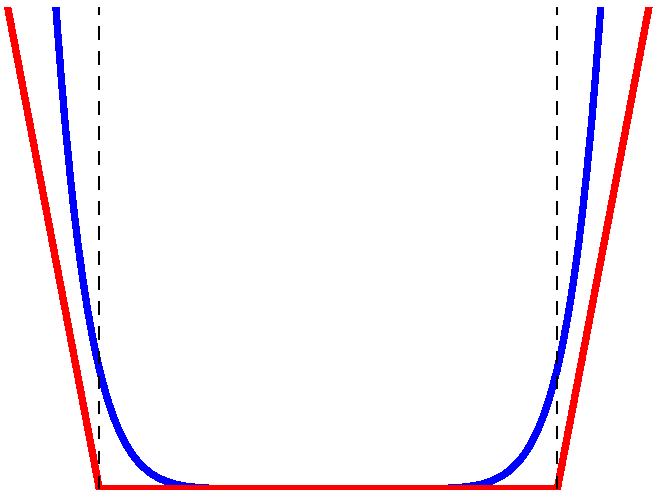
\includegraphics[scale=0.45]{figs/gpml/cost_barriers.pdf}};
\path[line] (-3.5,-1.95) -- (-3.5,2.2);
\path[line] (-3.6,-1.85) -- (3.6,-1.85);
\node at (3.5,-2.1) {$x$};
\node at (-1.5,-2.1) {$x_{\text{min}}$};
\node at (-3.0,2.1) {$c(x)$};
\node at (2,-2.1) {$x_{\text{max}}$};

\draw[dashed] (-3.5,-0.95) -- (3.4,-0.95);
\node at (-3.8,-0.95) {1};
\end{tikzpicture}
\caption{Barrier functions for which the expectation in \Eq{costint} can be evaluated analytically for $x \sim \cN$. These functions in are useful for penalising deviations outside of the set defined by $x_{\min}$ and $x_{\max}$. The polynomial is shown in blue and the affine is shown in red.}
\label{fig:cost_barriers}
\end{figure}
%-------------------------------------------------------------------------------------------------------------------------------------------


\subsection{Action Constraints} \label{sec:actioncon}

Constraints on the action space, again in the form of a convex polytope $\UU = \big\{\bu \in \RR^F \big| \bH\bu + \bh \in [-\mathbf{1},\mathbf{1}] \big\}$ parameterised by matrix $\bH \in \RR^{H\times F}$, can be addressed directly through the way in which the policy $\bpi$ is structured. Note that in this section $H$ shall denote the number of action constraints rather than the prediction horizon. A policy $\bpi: \RR^{E} \rightarrow \UU$ can be constructed in the following general form for $H \geq F$ linearly independent constraints
\begin{equation}
\bpi(\bx) = \bH^{\dagger} \mathrm{\mathbf{sat}}\big( \bH\tilde\bpi(\bx) + \bh \big) - \bH^{\dagger}\bh
\end{equation}
where $\bH^{\dagger} = (\bH\T\bH)\inv\bH\T$ is the right pseudo-inverse of $\bH$ and $\tilde\bpi: \RR^{E} \rightarrow \RR^F$ is a general unconstrained policy structure. The saturation function $\mathrm{\mathbf{sat}}: \RR^{H} \rightarrow \RR^{H}$ has elements
\begin{equation}
\mathrm{sat}^{(i)}(\bu) = \left\{ \begin{matrix}
-1 & \!\!\!\!\!\!\!\!\!\!\!\!\!\! \text{if } u^{(i)} \leq -1 \\
u^{(i)} & \text{if } -1 < u^{(i)} \leq 1 \\
1 & \!\!\!\!\!\!\!\!\!\!\!\!\!\!\!\!\!\! \text{if } u^{(i)} > 1
\end{matrix} \right.
\end{equation}
for $i \in \ZZ_{[1,H]}$. However, this will not fit into the moment matching framework since $\cov_{\bu}[\mathrm{\mathbf{sat}}(\bu)]$ for $\bu \sim \cN$ cannot be evaluated in closed form. Therefore this function is approximated using sinusoids, for which moment matching is possible. Two candidate approximations are
\begin{align}
s_1(u) &= \sin(u) \label{eqn:gsin} \\
s_2(u) &= \tfrac{9}{8}\sin\big(\tfrac{2}{3}u\big) + \tfrac{1}{8}\sin(2u) \label{eqn:gsat}
\end{align}
which are depicted in \Fig{sinsat}. Note that a standard Fourier series expansion would not be appropriate since the approximation must lie in the closed region $s_i(u) \in [-1,1]$ and have unit gradient at the origin $s'_i(0) = 1$ such that $\bpi(\bx) \approx \tilde\bpi(\bx)$ for $\bH\tilde\bpi(\bx) + \bh \approx \bO$. Again, defining the action constraints in this general way is also a contribution of this thesis.


%-------------------------------------------------------------------------------------------------------------------------------------------
\begin{figure}[t]
\centering
%
\tikzstyle{line} = [draw, -latex]
\begin{tikzpicture}
	\small
	\node at (0,0) {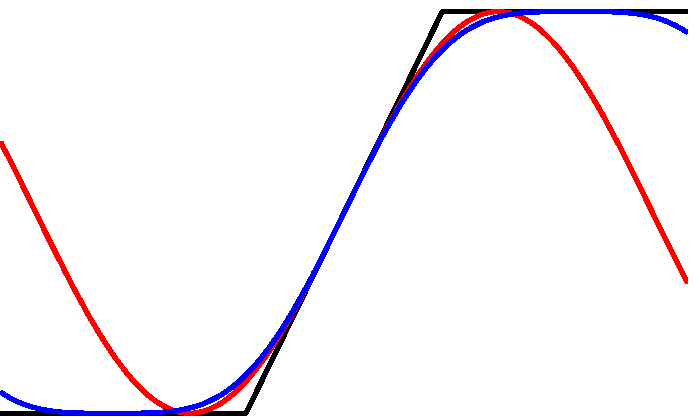
\includegraphics[scale=0.6]{figs/gpml/saturation.pdf}};
	\path[line] (0,-2.3) -- (0,2.3); \path[line] (-4,0) -- (4,0);
	\node at (3.8,-0.3) {$u$};
	\node at (3.8,2.3) {$\mathrm{sat}(u)$};
	\node at (3.8,1.5) {\color{blue}$s_2(u)$};
	\node at (3.8,-1) {\color{red}$s_1(u)$};
	
	\draw[dashed] (0.95,0) -- (0.95,2); \draw[dashed] (0,2) -- (0.95,2);
	\node at (0.95,-0.3) {1}; \node at (-0.3,2) {1};
	\draw[dashed] (-1.05,0) -- (-1.05,-2.07); \draw[dashed] (0,-2.07) -- (-1.1,-2.07);
	\node[fill=white] at (-1.05,-0.3) {-1}; \node[fill=white] at (-0.3,-2.07) {-1};
\end{tikzpicture}
%
\caption{Approximations to the $\mathrm{sat}$ function for which the expectation and covariance with respect to a Gaussian distributed input can be evaluated analytically. Specifically $s_1(u) = \sin(u)$ and $s_2(u) = \tfrac{9}{8}\sin\big(\tfrac{2}{3}u\big) + \tfrac{1}{8}\sin(2u)$. Both satisfy the conditions $s_i(u) \in [-1,1]$ and $s'_i(0) = 1$.}
\label{fig:sinsat}
\end{figure}
%-------------------------------------------------------------------------------------------------------------------------------------------


\section{Summary}
In this chapter we have defined the learning control framework, based on the algorithm of \cite{DR11}, that we shall use in the remainder of this thesis. We have outlined how Gaussian processes can be used as a probabilistic modelling tool for dynamical systems and how they can be used to obtain distributions over full trajectories in the state-action space. Kernels that can be used for defining distributions over linear systems, general additive systems and nonlinear systems have also been introduced. Finally, methods for handling state and action constraints have been given.


\chapter{M\lowercase{ultiple} D\lowercase{ynamics} M\lowercase{odels}} 

\section{Introduction}
We now begin to address the question of how to incorporate useful prior knowledge regarding the dynamics of a system into the probabilistic learning framework. In this chapter we deal with the problem of how to include known, or approximate, relationships between state variables. An important example of such a relationship is state variables that are related as time derivatives. In other words, position-velocity relationships. Another example would be higher order Markov systems where the system ``state" actually depends on a number of delayed ``states". Further, the task of tracking a known reference signal, or distribution of reference signals, could be contrived as a known relationship between state variables. With the probabilistic learning framework we have derived thus far, it is not clear how such information could be incorporated. We provide a novel method that tackles this problem.

%Often prior knowledge will come in the form of known, or approximate, relationships between a subset of the system state variables. In other words, the state-space may be partitioned into states with known dynamics and states with initially unknown dynamics. An obvious example of this is position-velocity relationships. However, more general problems may be tackled. The task of tracking a reference signal with a given linear combination of states in which the control policy may have access to some preview horizon of the reference can also be tackled by this framework. A further example is higher order Markov systems where the system ``state" actually depends on a number of delayed states.

Once we have formulated a method to achieve the goal of incorporating known state relationships we would like to investigate what effect their inclusion will have on learning. In particular we would like to investigate whether learning can proceed faster, both computationally and in terms of finding a good policy, and what is the propensity for finding good (or bad) local minima in completing the task.

Our method is formulated by considering that the system we are dealing with can be decomposed as multiple dynamics models all acting on different parts, or linear transformations, of the state-action vector. We shall use the terms \textit{multiple dynamics} and \textit{augmented dynamics} interchangeably when referring to this framework. In order to fit into the probabilistic framework, the use of multiple dynamics must satisfy the propagation of uncertainty criteria outlined in the previous chapter. It is this problem that we tackle now.


\section{Augmented Dynamics} \label{sec:augmentedDYN}
\subsection{Framework}

Consider the case in which the system dynamics function $\bff$ consists of the concatenation of $M$ distinct functions
\begin{equation}
\bff(\bz) = \bff_{1:M}(\bz) := \bmat{\bff_1(\bz) \\ \vdots \\ \bff_M(\bz)}
\label{eqn:multimodel}
\end{equation}
Each sub-function (or sub-dynamics) $\bff_m$ can explicitly depend on any of the previous functional outputs $\bff_{1:m-1}$ as well as the state-action $\bz$. In mathematical terms $\bff_m(\bz) = \bff_m\big(\bz,\bff_{1:m-1}(\bz)\big)$ for $m \in \ZZ_{[2,M]}$. We define the concatenation of the state-action and the $m-1$ previous functions as
\begin{equation*}
\bp_m(\bz) = \bmat{\bz \\ \bff_{1:m-1}(\bz) }
\end{equation*}
where $\bp_1(\bz) = \bz$ as this will be helpful later on. To see how this setup is beneficial for encoding position-velocity relationships or incorporating reference signals we show how they can be phrased in this framework using the following examples.

\begin{exa}[Position-Velocity] Consider a system with time derivative related states $\bx = [\ba; \dot\ba]$ where the positions $\ba$ evolve according to the dynamics $\ba_+ = \bff_1(\bz)$. The velocities $\dot\ba$ could then be reconstructed using some approximate relationship $\dot\ba_+ = \bff_2\big(\bz,\bff_1(\bz)\big)$, for example a linear relationship $\dot\ba_+ = \bM\big[\bz;\bff_1(\bz)\big]$. One setting for such a matrix could be $\bM = [-\bI, \bO, \bI]/\Dt$ which would encode the relationship $\dot\ba_+ = (\ba_+ - \ba)/\Dt$ which is reasonable for small $\Dt$. This example will be pursued further in \Sec{posvel}.
\end{exa}

\begin{exa}[Reference Generator] Consider a system with dynamics $\bx_+ = \bff_1(\bz)$ which has been tasked to track a some reference signal $\br$. Now assume that this reference comes from some underlying dynamical system $\bx^\br_+ = \bff_2(\bx^\br)$ where $\br = \bC^\br\bx^\br$. The dynamics of the system itself $\bx$ can then be augmented with the state of the reference system $\bx^\br$ such that the reference state simply becomes part of an augmented state space. Note that the function $\bff^\br$ could be provided by the user or inferred from data along with the system dynamics. How this setup can be used for learning reference tracking will be explored in \Sec{reffy}.
\end{exa}


In order to fit into the probabilistic framework of the previous chapter it is necessary for us to build up a moment-matched Gaussian approximation $\bff(\bz) \sim \cN(\bm_*, \bS_*)$ given $\bz \sim \cN(\bm,\bS)$. \Ass{gauss} states that $\bm_* = \EE_{\bz,\bff}[\bff(\bz)]$ and $\bS_* = \cov_{\bz,\bff}[\bff(\bz)]$. However, further approximations will have to be made in the case of multiple dynamics models since these moments cannot be calculated for general sub-functions even if the moments of each can be evaluated individually. 


\begin{ass} \label{ass:multigauss}
Given $p(\bz)$ is Gaussian, the resulting distribution of the next state $p\big(\bff(\bz)\big)$ is replaced by the Gaussian distribution
\begin{equation*}
\bff(\bz) \sim \cN\left(
\bmat{\EE_{\bz,\bff_1}[\bff_1(\bz)] \\ \vdots \\ \EE_{\brho_M,\bff_M}[\bff_M(\brho_M)]},
\bmat{\cov_{\bz,\bff_1}[\bff_1(\bz)] & \dots & \cov_{\brho_M,\bff_M}[\bff_1(\bz),\bff_M(\brho_M)] \\
\vdots & \ddots & \vdots \\
\cov_{\brho_M,\bff_M}[\bff_M(\brho_M),\bff_1(\bz)] & \dots & \cov_{\brho_M,\bff_M}[\bff_M(\brho_M)]}
\right)
\end{equation*}
where $p(\brho_m)$ is the moment matched approximation of the real distribution $p\big(\bp_m(\bz)\big)$.
\end{ass}

Note that this is an iterative extension of \Ass{gauss}. As before, we shall no longer make a distinction between the real distribution $p\big(\bp_m(\bz)\big)$ and its approximation $p(\brho_m)$.
%
Propagation of uncertainty is now reduced to the iterative procedure of evaluating the mean $\EE_{\bp_m,\bff_m}\big[\bff_m\big(\bp_m(\bz)\big)\big]$ and covariance $\cov_{\bp_m,\bff_m}\big[\bff_m\big(\bp_m(\bz)\big)\big]$ for each dynamics model, given the assumed joint Gaussian over the previous values $\bp_m(\bz) \sim \cN$. This is possible provided that these moments can be evaluated for each sub-dynamics.

Now in order to fill out the full covariance matrix, given \Ass{multigauss}, the cross terms $\cov_{\bp_m,\bff_m}\big[\bff_m\big(\bp_m(\bz)\big), \bp_m(\bz)\big]$ are required. It turns out that if the mean $\EE_{\bp_m,\bff_m}[\bff_m\big(\bp_m(\bz)\big)]$ is differentiable with respect to the input mean $\bm = \EE_{\bp_m}[\bp_m(\bz)]$ then this term can always be evaluated as
%
\begin{align}
\cov_{\bp_m,\bff_m}\big[\bff_m\big(\bp_m(\bz)\big), \bp_m(\bz)\big] &= \bigg(\diff{}{ \bm } \EE_{\bp_m,\bff_m}\big[\bff_m\big(\bp_m(\bz)\big)\big] \bigg) \bS
\label{eqn:multicov}
\end{align}
%
where $\bS = \cov_{\bp_m}[\bp_m(\bz)]$ is the input covariance. This expression holds due to \Theo{inpout}. This theorem lies at the heart of the multi-model framework. While it is a straightforward derivation, this result was unknown to us from the literature, therefore the derivation is our own.


\begin{theo}[Output-Input Covariance] \label{theo:inpout}
Consider two random vectors $\ba$ and $\bb$ where $\bb$ is functionally dependent on $\ba \sim \cN(\bm,\bS)$. Then the following statement is true
\begin{equation*}
\diff{}{ \bm }\EE_{\ba,\bb}[\bb] =  \cov_{\ba,\bb}[\bb,\ba] \bS^{-1}
\end{equation*}
\espa
\end{theo}



\begin{proof}
The proof follows directly from the definition of expectation and covariance
\begin{align*}
\diff{}{\bm}\EE_{\ba,\bb}[\bb]
&= \int \EE_{\bb}[\bb] \bigg( \diff{}{\bm} \cN\big(\ba|\bm,\bS\big) \bigg) \dd\ba  \\
&= \int \EE_{\bb}[\bb] \Big(  (\ba - \bm)\T \bS^{-1} \cN\big(\ba|\bm,\bS\big) \Big) \dd\ba
\end{align*}
Now expanding out the brackets yields the expression
\begin{flalign*}
\qquad\qquad\qquad\qquad\quad\;\;
\diff{}{\bm}\EE_{\ba,\bb}[\bb]
&= \bigg( \EE_{\ba,\bb}[\bb \ba\T] - \EE_{\ba,\bb}[\bb] \bm\T \bigg) \bS^{-1}   \\ &
= \cov_{\ba,\bb}[\bb,\ba] \bS^{-1} & \blacksquare
\end{flalign*}
\end{proof}

Note that the assumption of joint Gaussianity is equivalent to assuming linear relationships between dynamics models. To see this, observe that \Eq{multicov} is in the form of a Jacobian matrix (or linearised dynamics) multiplied by the input covariance.





\subsection{Subset of Inputs}
Often the case will be that each dynamics model is only functionally dependent on a subset, or linear transformation, $\bs_m(\bz)$ of the state-actions and outputs of previous functions $\bp_m(\bz)$. How then is the expectation and covariance with respect to $\bp_m(\bz)$ to be filled in? The answer can be found by considering the general linear transformation $\bs_m(\bz) = \bP_m\bp_m(\bz)$. The matrix $\bP_m$ could either pick off appropriate elements of $\bp_m$ or be viewed as an arbitrary linear combination. Since this mapping is linear, a Gaussian distribution $\bp_m(\bz) \sim \cN(\bm,\bS)$ leads to another Gaussian distribution $\bs_m(\bz) \sim \cN\big(\bm_{\bs},\bS_{\bs}\big)$ with mean $\bm_{\bs} = \bP_m\bm$ and covariance $\bS_{\bs} = \bP_m\bS\bP_m\T$. Therefore the predictive mean and covariance are simply
\begin{align*}
\EE_{\bp_m,\bff_m}\big[\bff_m\big(\bp_m(\bz)\big)\big] &= \EE_{\bs_m,\bff_m}\big[\bff_m(\bs_m(\bz)\big)\big] \\
\cov_{\bp_m,\bff_m}\big[\bff_m\big(\bp_m(\bz)\big)\big] &= \cov_{\bs_m,\bff_m}\big[\bff_m\big(\bs_m(\bz)\big)\big]
\end{align*}
In order to obtain the cross covariance term $\cov_{\bp_m,\bff_m}\big[\bff_m\big(\bp_m(\bz)\big), \bp_m(\bz)\big] = \cov_{\ba,\bb}[\bb,\ba]$ first define $\bc = \bs_m(\bz)$. Then note that, since $\bb$ is only affected by $\ba$ through $\bc$, the conditional independence relationship $\ba \ci \bb | \bc$ holds. This relationship can be represented by the graphical model shown in \Fig{condind}. Due to the joint Gaussian assumption, \Theo{condind} can be appealed to. This theorem is well known in the Machine Learning community.






%-------------------------------------------------------------------------------------------------------------------------------------------
\begin{figure}[t]
\centering
%
\tikzstyle{sum} = [circle, draw, minimum height=.8cm]
\tikzstyle{line} = [draw, -latex]
\begin{tikzpicture}
	\node[sum] (a) at (-2,0) {$\ba$}; 
	\node[sum] (b) at (0,-1) {$\bc$};
	\node[sum] (c) at (2,0) {$\bb$};
	\path[line] (a) -- (b); \path[line] (b) -- (c);
\end{tikzpicture}
%
\caption{Graphical model for which the conditional independence relationship $\ba \ci \bb \big| \bc$ holds. See \cite{Bish06} Chapter 8.2 for a more detailed outline.}
\label{fig:condind}
\end{figure}
%-------------------------------------------------------------------------------------------------------------------------------------------





\begin{theo}[Conditional Independence] \label{theo:condind}
Take three random vectors $\ba,\bb$ and $\bc$ which are jointly Gaussian distributed. Given $\ba \ci \bb | \bc$ the following statement is true
\begin{equation*}
\cov[\bb,\ba] = \cov[\bb,\bc] \cov[\bc]^{-1} \cov[\bc,\ba]
\end{equation*}
\end{theo}

\begin{proof}
Consider the joint distribution $p(\ba,\bb,\bc)$ partitioned as follows
\begin{equation*}
\bmat{\ba \\ \bb \\ \bc} \sim \cN \left(
\bmat{\bm_{\ba} \\ \bm_{\bb} \\ \bm_{\bc}},
\bmat{
\bS_{\ba} & \bS_{\ba\bb} & \bS_{\ba\bc} \\
\bS_{\bb\ba} & \bS_{\bb} & \bS_{\bb\bc} \\
\bS_{\bc\ba} & \bS_{\bc\bb} & \bS_{\bc}
} \right)
\end{equation*}
Conditioning $\ba$ and $\bb$ on $\bc$ using the identity for a Gaussian conditional distribution yields the cross covariance term
\begin{equation*}
\cov[\bb,\ba|\bc] = \bS_{\bb\ba} - \bS_{\bb\bc} \bS_{\bc}^{-1} \bS_{\bc\ba}
\end{equation*}
This expression is equal to zero since the conditional independence relationship $\ba \ci \bb | \bc$ can be stated equivalently as $\cov[\ba,\bb|\bc] = \bO$. The result follows from a rearrangement of terms.
\qed
\end{proof}

However, computing the inverse of the potentially singular matrix $\cov[\bc]$ is unsatisfactory. Fortunately, explicit calculation of this inversion is unnecessary since $\cov[\bb,\bc] \bS_{\bs}^{-1} = \dd\EE[\bb]/\dd\bm_{\bs}$ due to \Theo{inpout}. Therefore the cross covariances can be expressed as
\begin{align*}
\cov_{\bp_m,\bff_m}\big[\bff_m\big(\bp_m(\bz)\big), \bp_m(\bz)\big]
&= \bigg(\diff{}{ \bm_{\bs} } \EE_{\bs_m,\bff_m}[\bff_m\big(\bs_m(\bz)\big)\big] \bigg) \bP_m \bS
\end{align*}
where $\bP_m\bS = \cov[\bc,\ba]$. The full framework for propagating uncertainty using multiple dynamics models was implemented in MATLAB and can be found in \App{codeCost} implemented by the function \texttt{propagated.m}. This function has been developed by multiple contributors where the author's main contributions to it were the multiple dynamics framework and the derivative calculations using the vectorisation convention of \App{matcal}.

This concludes the definition of the framework for propagation of Gaussian uncertainty given multiple dynamics models with the form in \Eq{multimodel}. Note that the only condition on each dynamics model is that the mean $\EE_{\bs_m,\bff_m}\big[\bff_m\big(\bs_m(\bz)\big)\big]$ and covariance $\cov_{\bs_m,\bff_m}\big[\bff_m\big(\bs_m(\bz)\big)\big]$ are analytically tractable for $\bs_m \sim \cN$, $\bff_m \sim \mathcal{GP}$ and that the mean is differentiable with respect to the mean of the input distribution $\bm_{\bs}$. Now some specific applications are discussed.


\subsection{Higher Order Markov Systems} \label{sec:nonmarkov}
One use of this framework that is immediately transparent is the case in which the system in question has a Markov order greater than one in its relationship to previous states. In other words, with multiple dynamics models, Markov system of order $N$ and of the form
\begin{equation*}
\bx_{k+1} = \bff\big(\bx_{k},\bx_{k-1}\dots,\bx_{k-N+1},\bu_{k}\big)
\end{equation*}
can be considered by defining the augmented state-space system
\begin{equation*}
\bx^{\aug}_{k+1} = \bmat{ \bff\big(\bx^{\aug}_{k},\bu_{k}\big) \\[0.1cm] 
\bmat{\bI & \bO} \bx^{\aug}_{k}
}
\end{equation*}
with augmented state vector $\bx^{\aug}_k = [\bx_{k}; \bx_{k-1} \dots  \bx_{k-N+1}] \in \RR^{NE}$. Obviously a similar procedure could be applied if the system also depends on delayed actions. This is a useful property that we will exploit in the subsequent sections.







\section{Known State Relationships}

\subsection{General Mappings}
The framework of multiple dynamics models outlined in the previous section finds one of its most useful applications in the incorporation of known relationships between states, a form of partial model information. This application is presented in \cite{HRM12}. Specifically, given a system composed of $M$ distinct functions as given in \Eq{multimodel}, then often some of the sub-dynamics may be fixed or known beforehand. In this case, the unknown dynamics can be inferred from data using a parametric or nonparametric method outlined in \Sec{bayesmodelling} while the known parts can be included directly. A very clear and useful example of this for dynamical systems is the case where some states are known to be time derivatives of other states. In other words, position-velocity relationships.









\subsection{Position-Velocity}
\label{sec:posvel}




Consider the common scenario in which the state $\bx$ contains \textit{position} states $\bxp$ and \textit{velocity} states $\bxv$ which are related through
\begin{align}
\bxp_k &= \int_{-\infty}^t \!\!\!\!\bxv(\tau) \dd\tau \quad\text{or}\quad
\bxp_k = \bxp_{k-1} + \int_{t-\Dt}^t \!\!\!\!\bxv(\tau) \dd\tau \label{eqn:posint} \\[0.2cm]
\bxv_k &= \frac{\dd\bxp(\tau)}{\dd \tau} \bigg|_{\tau = t} \label{eqn:veldiff}
\end{align}
where $k \in \ZZ$ and $t = k\Dt$. In order to incorporate this information into the learning framework it is important to first determine whether a predictive model for the position states is to be inferred and the velocity states reconstructed from this prediction (numerical differentiation) or vice versa (numerical integration). Approximate solutions for both cases will be discussed.



%-------------------------------------------------------------------------------------------------------------------------------------------
\begin{figure}
\centering
%
\subfigure[Integral approximations.]{
\begin{tikzpicture}
	\small
	\node at (0,0) {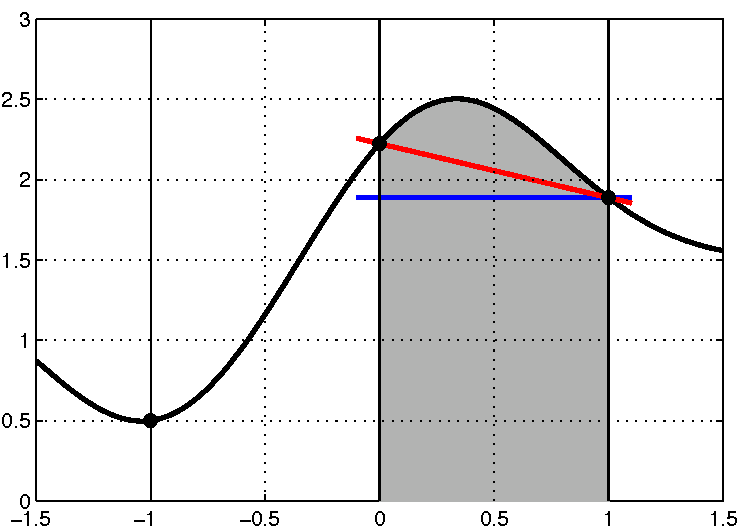
\includegraphics[scale=0.6, clip, trim=0.5cm 0.4cm 0cm 0cm]{figs/prioraug/vp1.pdf}};
	\node at (2.3,-2.8) {$t$}; \node at (3.0,-2.79) {time};
	\node at (0,-2.8) {$t-\Dt$};
	\node at (-2.3,-2.8) {$t-2\Dt$};
	\node[rotate=90] at (-3.05,1.3) {velocity $\bxv$};
	\node at (1.15,-1) {$\int_{t-\Dt}^t \bxv \dd\tau$};
\end{tikzpicture}
\label{fig:posint}
}
\hfill
\subfigure[Derivative approximations.]{
\begin{tikzpicture}
	\small
	\node at (0,0) {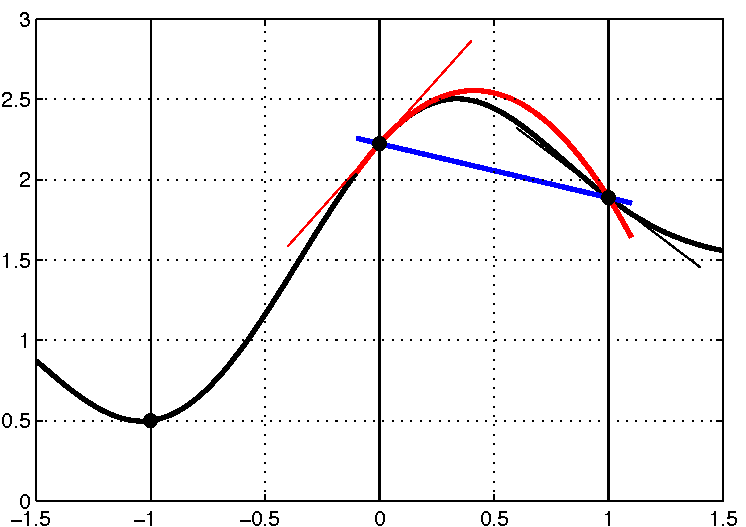
\includegraphics[scale=0.6, clip, trim=0.5cm 0.4cm 0cm 0cm]{figs/prioraug/vp2.pdf}};
	\node at (2.3,-2.8) {$t$}; \node at (3.0,-2.79) {time};
	\node at (0,-2.8) {$t-\Dt$};
	\node at (-2.3,-2.8) {$t-2\Dt$};
	\node[rotate=90] at (-3.05,1.3) {position $\bxp$};
	\node at (2.85,-0.4) {$\frac{\dd\bxp}{\dd \tau}(t)$};
\end{tikzpicture}
\label{fig:veldiff}
}
%
\caption{Approximate reconstruction of the current position/velocity states given previous observations of the velocity/position states up to time $t-\Dt$. The thick blue and red lines in each plot make approximations of zero and constant acceleration $\dot\bx^{\text{v}}$ respectively. The thin red line in plot (b) shows actual gradient at time $t-\Dt$, which the constant acceleration approximation utilises.}
\end{figure}
%-------------------------------------------------------------------------------------------------------------------------------------------


First consider the reconstruction of the position states $\bxp_k$ given the previous position $\bxp_{k-1}$ and the set of inferred velocities $\bxv_k$ and $\bxv_{k-1}$ from the probabilistic model. This corresponds to approximating the integral in \Eq{posint} which is depicted graphically in \Fig{posint}. Assuming the velocity follows a constant or linear variation (equivalently the acceleration is zero or constant across the interval) corresponds to the following approximations
\begin{align}
\bxp_k &\approx \bxp_{k-1} + \Dt\bxv_k \label{eqn:int1} \\
\bxp_k &\approx \bxp_{k-1} + \tfrac{1}{2} \Dt \Big( \bxv_k + \bxv_{k-1} \Big) \label{eqn:int2}
\end{align}
respectively. These are roughly equivalent to the Euler and Heun methods for numerical integration. Now consider reconstruction of the velocity states $\bxv_k$ given the inferred positions $\bxp_k$ and $\bxp_{k-1}$. In this case assuming the position follows a linear or quadratic variation (equivalently the acceleration is zero or constant across the interval) leads to
\begin{align}
\bxv_k &\approx \Dt\inv \Big( \bxp_k - \bxp_{k-1} \Big) \label{eqn:diff1} \\
\bxv_k &\approx 2 \Dt\inv \Big( \bxp_k - \bxp_{k-1} \Big) - \bxv_{k-1} \label{eqn:diff2}
\end{align}
respectively. This process is depicted in \Fig{veldiff}. As expected, these relationships are simply rearrangements of \Eqs{int1}{int2}. All these approximate relationships are linear and can therefore be easily incorporated into the multiple dynamics framework.






%-------------------------------------------------------------------------------------------------------------------------------------------
\begin{figure}[t]
\centering
%
\subfigure[Integral approximations.]{
\tikzstyle{line} = [draw, -stealth']
\begin{tikzpicture}
	\small
	\node at (0,0) {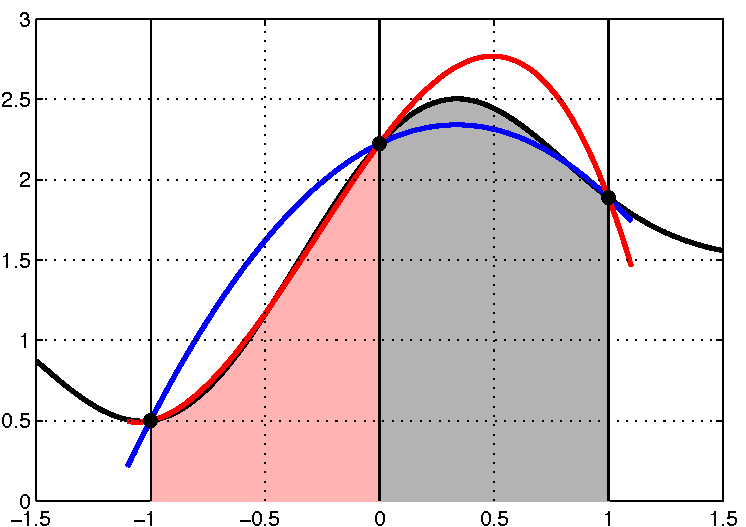
\includegraphics[scale=0.6, clip, trim=0.5cm 0.4cm 0cm 0cm]{figs/prioraug/vp3.pdf}};
	\node at (2.3,-2.8) {$t$}; \node at (3.0,-2.79) {time};
	\node at (0,-2.8) {$t-\Dt$};
	\node at (-2.3,-2.8) {$t-2\Dt$};
	\node[rotate=90] at (-3.05,1.3) {velocity $\bxv$};
	\node at (1.15,-1) {$\int_{t-\Dt}^t \bxv \dd\tau$};
\end{tikzpicture}
\label{fig:posint2}
}
%
\subfigure[Derivative approximations.]{
\tikzstyle{line} = [draw, -stealth']
\begin{tikzpicture}
	\small
	\node at (0,0) {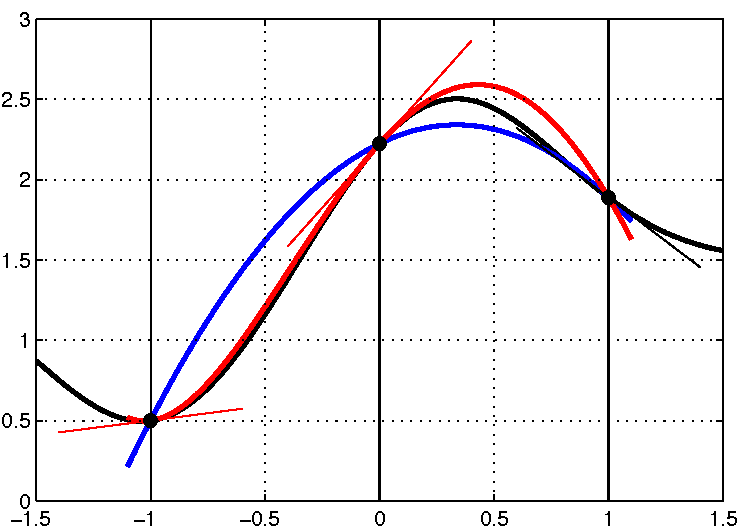
\includegraphics[scale=0.6, clip, trim=0.5cm 0.4cm 0cm 0cm]{figs/prioraug/vp4.pdf}};
	\node at (2.3,-2.8) {$t$}; \node at (3.0,-2.79) {time};
	\node at (0,-2.8) {$t-\Dt$};
	\node at (-2.3,-2.8) {$t-2\Dt$};
	\node[rotate=90] at (-3.05,1.3) {position $\bxp$};
	\node at (2.85,-0.4) {$\frac{\dd\bxp}{\dd \tau}(t)$};
\end{tikzpicture}
\label{fig:veldiff2}
}
%
\caption{Approximate reconstruction of the current position/velocity states given previous observations of the velocity/position states up to time $t-2\Dt$. The blue lines in plot (a) and (b) use only the three observed points on the graph to make a quadratic approximation of the actual curve. The red line in plot (a) additionally uses the red shaded area $\int \bxv \dd\tau$ over $[t-2\Dt,t-\Dt]$ to form a cubic approximation. This is equivalent to the red line in plot (b) which uses the derivatives $\frac{\dd\bxp}{\dd \tau}(t-\Dt)$ and $\frac{\dd\bxp}{\dd \tau} (t-2\Dt)$ shown by thin red lines to make a quartic approximation.}
\label{fig:posvel2}
\end{figure}
%-------------------------------------------------------------------------------------------------------------------------------------------





As discussed in \Sec{nonmarkov} it is not a problem to form dependencies on delayed states $\bx_{k-i}$ for $i >1$. Therefore, more elaborate approximations can be made by using information from previous timesteps. For example, fitting a quadratic curve to the points $\bxv_k, \bxv_{k-1}, \bxv_{k-2}$ or fitting a cubic curve to these points and given the area defined by $\bxp_{k-1} - \bxp_{k-2}$ yields the following approximations
\begin{align}
\bxp_{k} &\approx \bxp_{k-1} + \tfrac{1}{12}\Dt\Big( 5\bxv_k + 8\bxv_{k-1} - \bxv_{k-2} \Big) \label{eqn:dada} \\
\bxp_{k} &\approx \bxp_{k-2} + \tfrac{1}{3}\Dt\Big( \bxv_k + 4\bxv_{k-1} + \bxv_{k-2} \Big) \label{eqn:mama}
\end{align}
for position reconstruction. These approximations are shown in \Fig{posint2} by the blue and red curves respectively. Note that since there are four constraints that must be satisfied then a cubic function can do this uniquely since it has four degrees of freedom. Lower order polynomials could also be considered which would yield a unique analytic solution but would not guarantee satisfaction of the constraints.

Now, in terms of velocity reconstruction, a quadratic fit to the points $\bxp_k, \bxp_{k-1}, \bxp_{k-2}$ and a quartic fit to these points plus the derivatives defined by $\bxv_{k-1}$ and $\bxv_{k-2}$ give the relationships
\begin{align}
\bxv_{k} &\approx \tfrac{1}{2} \Dt\inv \Big( 3\bxp_{k} - 4\bxp_{k-1} + \bxp_{k-2} \Big) \label{eqn:dada2} \\
\bxv_{k} &\approx 3\Dt\inv \Big( \bxp_k - \bxp_{k-2} \Big) - \Big( 4\bxv_{k-1} + \bxv_{k-2} \Big) \label{eqn:mama2}
\end{align}
Note that the cubic fit to the velocity profile in \Eq{mama} is equivalent to the quartic fit to the position profile in \Eq{mama2}. These approximations are shown in \Fig{veldiff2} by the blue and red curves respectively.

It is important to note that using additional information from previous timesteps and higher order polynomials will not necessarily give better approximations of the integral or derivative. This is clearly shown in \Fig{posvel2} where we see that the higher order polynomial fit (thick red lines) produces a worse approximation of the required integral and derivative than the lower order fit (thick blue lines). We shall see in the following experiments whether this issue occurs in practice.


\subsection{Example: Pendulum} \label{sec:pendulum}

%-------------------------------------------------------------------------------------------------------------------------------------------
\begin{figure}
\centering
\small
\begin{tikzpicture}[]
	\draw[dashed] (0,0) circle (3cm);
	\draw[line width=1.2mm, rotate=45] (0,0) -- (0,-3);
	\draw[dashed] (0,0) -- (0,-3);
	\draw[rotate=-90,-latex,thick] (1,0) arc (0:45:1cm);
	\draw[-latex,thick,red] (-0.3536,0.3536) arc (-225:45:0.5cm); % 0.5/sqrt(2)
	\draw[fill=gray] (0,0) circle (1mm);
	\draw[fill=gray,rotate=45] (0,-3) circle (1mm);
	
	\node[] at (0.4,-1.2) {$\theta$};
	\node[] at (1.3,-0.7) {$l$};
	\node[] at (-0.7,0) {\color{red} $u$};
	
	\draw[xshift=0.3cm,rotate=-45,-latex, thick] (0,0) -- (2.8,0);
	\draw[xshift=0.3cm,rotate=-45,-latex, thick] (0.1,0) -- (-0.2,0);
	\draw[very thick, blue] (0,2.85) -- (0,3.15); \draw[very thick, blue] (0.15,3) -- (-0.15,3);
\end{tikzpicture}
\caption{Torque-limited pendulum with angle from the down position $\theta$, length $l$ and input torque $u$.}
\label{fig:pendulum}
\end{figure}
%-------------------------------------------------------------------------------------------------------------------------------------------



\subsubsection{Setup}
In order to analyse these approximation schemes, the torque-limited pendulum swing up problem was considered. This simple system is shown in \Fig{pendulum} where the pendulum is considered to be a pole of uniform density. The equation of motion for this system is therefore given by
\begin{equation*}
\tfrac{1}{3}ml^2 \ddot{\theta} = u - b\dot\theta - \tfrac{1}{2}mlg\sin\theta
\end{equation*}
The constants we used can be found in \App{pend}. The input torque $u$ is constrained and is insufficient to swing the pendulum up directly.
%
The cost function used for learning was the angular distance to the upright position $c(\bx) = \half(\cos\theta+1) \in [0,1]$. This cost makes no distinction between swinging the pendulum up to $\theta=\pi$ or $\theta=-\pi$. The prediction horizon was set to $T = 3\,$s with a discrete timestep $\Dt = 0.1\,$s. Note that this discretisation is relatively short given that the natural period of the pendulum is $T_0 = 2\pi/\omega_0 \approx 1.6\,$s where $\omega_0 = \sqrt{3g/2l}$.
The control policy was a radial basis function with 50 Gaussian kernels in which the positions, widths and magnitudes of each kernel were free to be optimised. The output of this policy was then passed through the approximate saturating block defined in \Eq{gsat} in order to satisfy the action constraints. 


The algorithm was given two independent Gaussian processes with squared exponential kernels to learn the unknown system dynamics. We tasked these GPs to learn a mapping from $[\dot\theta_{k-1}$, $\sin\theta_{k-1}, \cos\theta_{k-1}]\T$ to the differences $(\theta_k-\theta_{k-1})$ and $(\dot\theta_k-\dot\theta_{k-1})$. This input representation was chosen to encode the fact that the angle $\theta$ is the same as the angle $\theta+2\pi$. Differences were predicted so that a zero mean prior would be suitable. Of course this equivalent to incorporating a fixed linear mean function. The input representation at the following timestep $[\dot\theta_{k}$, $\sin\theta_{k}, \cos\theta_{k}]\T$ could then be reconstructed using linear and trigonometric relationships, which satisfy the criteria for the moment matching approximation.
%
The learned dynamics were then initialised with a training data set of 3$\,$s which was obtained by applying random inputs to the pendulum starting with it hanging down.

This is an interesting problem due to the existence of locally optimal solutions. The optimal solution consists of a single swing back followed by the swing to the upright position. This can be verified, for example, by Dynamic Programming. However other solutions involving multiple swings or swinging the pendulum round and round many times also exist. We will investigate the propensity for the algorithm to fall into one of these locally optimal solutions in the presence of approximate models for the position-velocity relationship.




%-------------------------------------------------------------------------------------------------------------------------------------------
\begin{figure}
\centering \small
\subfigure[Distribution of costs after each iteration]{
\tikzstyle{sum} = [rectangle, draw, rounded corners, minimum height=0.38cm, text width = 1.0cm]
\begin{tikzpicture}
  \node at (0,0) {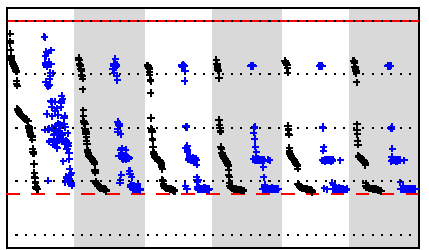
\includegraphics[scale = 1.0]{figs/prioraug/intdiff_heu1.pdf}};
  \node at (0,-2.8) {Algorithm Iteration};
  \node at (-2.9,-2.35) {1};
  \node at (-1.74,-2.35) {2};
  \node at (-0.58,-2.35) {3};
  \node at (0.58,-2.35) {4};
  \node at (1.74,-2.35) {5};
  \node at (2.9,-2.35) {6};
  \node[rotate=90] at (-3.85,0) {Cost};
  \node at (-3.85,1.75) {1.0};
  \node at (-3.85,-1.8) {0.2};
  \node[sum,red,line width=1.8pt] at (2.88,1.0) {};
  \node[sum,black,line width=1.8pt] at (2.88,-0.6) {};
  \node[sum,blue,line width=1.8pt] at (2.88,-1.1) {};
  \node at (0,-2.5) {};
\end{tikzpicture}
\label{fig:standi1}
}
\hspace{1cm}
\subfigure[Three locally optimal solutions]{
\begin{tikzpicture}
  \node at (0,0) {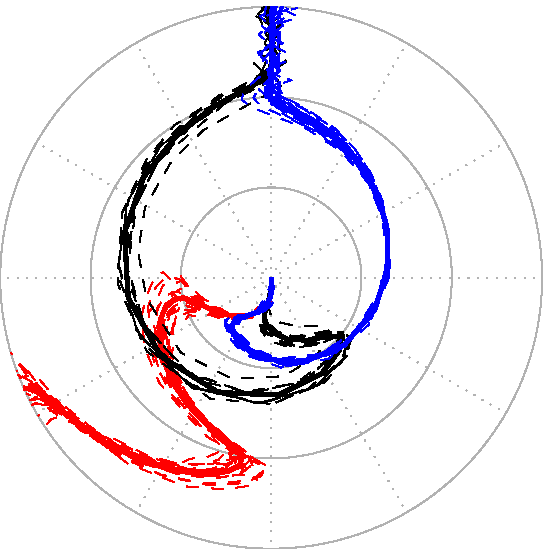
\includegraphics[scale = 0.5]{figs/prioraug/nifty.pdf}};
  \node at (0.65,0.65) {\footnotesize 1$\,$s};
  \node at (1.25,1.25) {\footnotesize 2$\,$s};
  \node at (1.79,1.79) {\footnotesize 3$\,$s};
  \node at (0,-2.55) {down};
  \node at (0,2.55) {upright};
\end{tikzpicture}
\label{fig:standj1}
}
\caption{The graph in (a) depicts the cost trajectories over six iterations of 50 Monte Carlo runs of the standard learning algorithm to the pendulum problem. The black crosses show the actual costs incurred and the blue crosses show the associated mean predicted costs. The maximum cost and the global optimum are shown by the red line and the red dashed line respectively. The three solutions that the algorithm tended to settle for are shown by the trajectories in (b). The blue is close the global optimum solution, consisting of a single swing-back, while the black is a local optimum consisting of two swings. Finally, the red is a locally optimal solution of simply applying full actuation torque over the whole horizon.}
\label{fig:stand1}
\end{figure}
%-------------------------------------------------------------------------------------------------------------------------------------------




\subsubsection{Standard Method}
The results of applying the learning algorithm of \cite{DR11}, which we shall refer to as the ``standard method", to the pendulum are shown in \Fig{standi1}. This is clearly a relatively easy task in terms of system identification since the predicted costs match the actual costs after only two iterations (6$\,$s of data). In terms of learning the control task, many of the runs can learn a policy that works after just the first iteration (3$\,$s of data) while the majority of runs achieve the swing up task by the second iteration.

What makes this an interesting problem is not the learning speed but that there are clearly three solutions in which the algorithm gets stuck. Note that the algorithm was run as long as 10 iterations and the distribution of solutions did not change. The three locally optimal solutions are shown in \Fig{standj1}. The first, shown in blue, is an ideal solution consisting of a single-swing back before the swing-up. This is close to the theoretical limit, shown by the dashed red line.
% and determined through dynamic programming. 
It is desirable for all runs to end up here. The second mode, shown in black, is a locally optimal solution consisting of two swings before the swing-up. Finally, there is a common failure mode shown in red in which the policy simply applies the maximum control action over the whole horizon and gets stuck here.








%-------------------------------------------------------------------------------------------------------------------------------------------
\begin{figure*}
\centering \footnotesize
\subfigure[Use GPs to learn evolution of both $\theta$ and $\dot\theta$.]{ % Uncertainty in theta
\begin{tikzpicture}
  \node at (5.2,0) {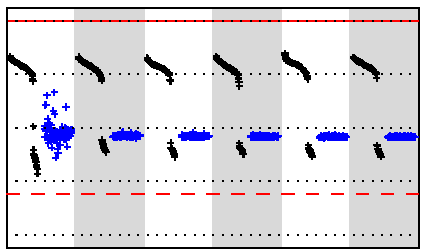
\includegraphics[scale = 0.7]{figs/prioraug/addnoise1.pdf}};
  \node at (0,0) {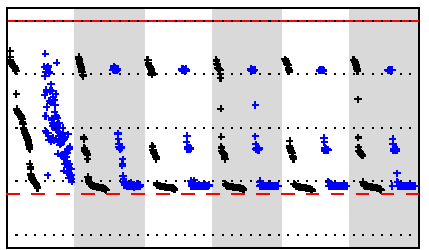
\includegraphics[scale = 0.7]{figs/prioraug/addnoise2.pdf}};
  \node at (-5.2,0) {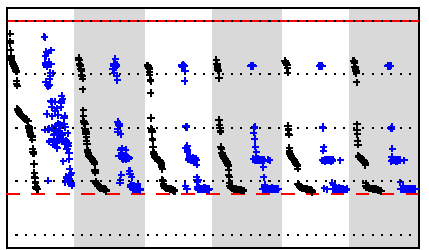
\includegraphics[scale = 0.7]{figs/prioraug/intdiff_heu1.pdf}};
  \node[rotate=90] at (-8.0,0) {Cost};
  \node at (-8.0,1.25) {1.0};
  \node at (-8.0,-1.25) {0.2};
  \node[fill=white,rounded corners] at (-3.5,-1.15) {\scriptsize $\sigma^2 = 0$};
  \node[fill=white,rounded corners] at (1.6,-1.15) {\scriptsize $\sigma^2 = 0.01$};
  \node[fill=white,rounded corners] at (6.85,-1.15) {\scriptsize $\sigma^2 = 0.1$};
\end{tikzpicture}
\label{fig:noisy1}
} 
\subfigure[Reconstruct $\theta$ using the Euler method.]{ % Uncertainty in dtheta
\begin{tikzpicture}
  \node at (5.2,0) {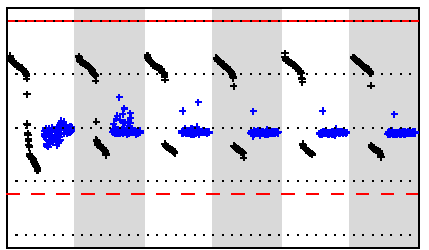
\includegraphics[scale = 0.7]{figs/prioraug/intdiff_eul2.pdf}};
  \node at (0,0) {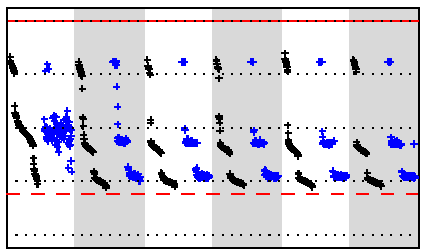
\includegraphics[scale = 0.7]{figs/prioraug/intdiff_eul3.pdf}};
  \node at (-5.2,0) {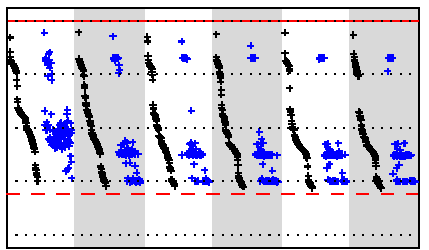
\includegraphics[scale = 0.7]{figs/prioraug/intdiff_eul5.pdf}};
  \node[rotate=90] at (-8.0,0) {Cost};
  \node at (-8.0,1.25) {1.0};
  \node at (-8.0,-1.25) {0.2};
  \node[fill=white,rounded corners] at (-3.5,-1.15) {\scriptsize $\sigma^2 = 0$};
  \node[fill=white,rounded corners] at (1.6,-1.15) {\scriptsize $\sigma^2 = 0.01$};
  \node[fill=white,rounded corners] at (6.85,-1.15) {\scriptsize $\sigma^2 = 0.1$};
\end{tikzpicture}
\label{fig:eul1}
}
\subfigure[Reconstruct $\theta$ using the Heun method.]{ % Uncertainty in dtheta
\begin{tikzpicture}
  \node at (5.2,0) {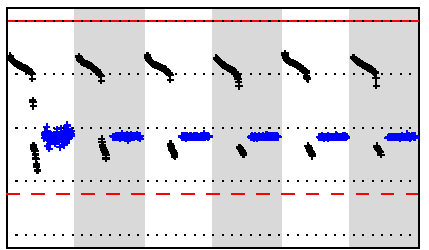
\includegraphics[scale = 0.7]{figs/prioraug/intdiff_heu2.pdf}};
  \node at (0,0) {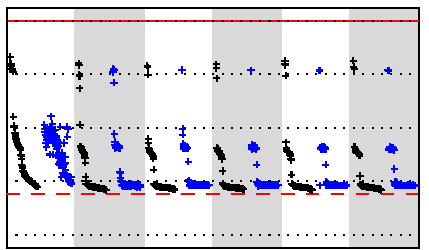
\includegraphics[scale = 0.7]{figs/prioraug/intdiff_heu3.pdf}};
  \node at (-5.2,0) {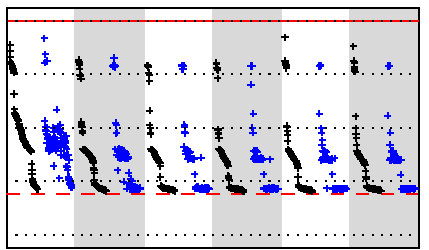
\includegraphics[scale = 0.7]{figs/prioraug/intdiff_heu5.pdf}};
  \node[rotate=90] at (-8.0,0) {Cost};
  \node at (-8.0,1.25) {1.0};
  \node at (-8.0,-1.25) {0.2};
  \node[fill=white,rounded corners] at (-3.5,-1.15) {\scriptsize $\sigma^2 = 0$};
  \node[fill=white,rounded corners] at (1.6,-1.15) {\scriptsize $\sigma^2 = 0.01$};
  \node[fill=white,rounded corners] at (6.85,-1.15) {\scriptsize $\sigma^2 = 0.1$};
\end{tikzpicture}
\label{fig:heu1}
}
\subfigure[Reconstruct $\theta$ using the Cubic method.]{ % Uncertainty in dtheta
\begin{tikzpicture}
  \node at (5.2,0) {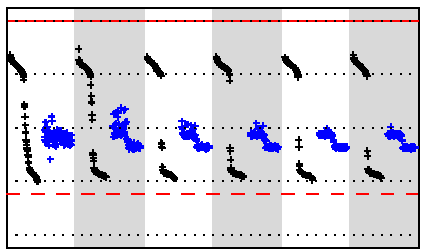
\includegraphics[scale = 0.7]{figs/prioraug/intdiff_fan2.pdf}};
  \node at (0,0) {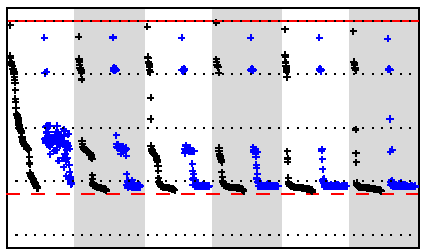
\includegraphics[scale = 0.7]{figs/prioraug/intdiff_fan3.pdf}};
  \node at (-5.2,0) {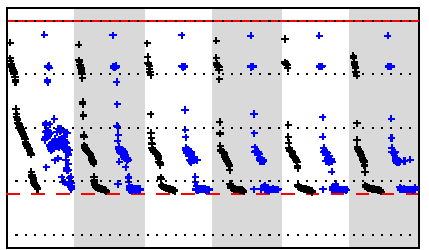
\includegraphics[scale = 0.7]{figs/prioraug/intdiff_fan5.pdf}};
  \node[rotate=90] at (-8.0,0) {Cost};
  \node at (-8.0,1.25) {1.0};
  \node at (-8.0,-1.25) {0.2};
  \node[fill=white,rounded corners] at (-3.5,-1.15) {\scriptsize $\sigma^2 = 0$};
  \node[fill=white,rounded corners] at (1.6,-1.15) {\scriptsize $\sigma^2 = 0.01$};
  \node[fill=white,rounded corners] at (6.85,-1.15) {\scriptsize $\sigma^2 = 0.1$};
\end{tikzpicture}
\label{fig:cub1}
}
\caption{Plots of the distribution of actual costs (black) and the mean predicted cost (blue) for different levels of additive noise $\cN(\bO,\sigma^2\bI)$ on the prediction of $\theta$. The x-axis displays the algorithm iteration and the y-axis shows the cost $J(\bpsi)$. These plots were constructed from 100 Monte Carlo runs with initial training data sets obtained by applying different random torque actions.}
\label{fig:integ}
\end{figure*}
%-------------------------------------------------------------------------------------------------------------------------------------------








\subsubsection{Position Reconstruction}
The explicit inclusion of approximate position-velocity information in the pendulum swing-up problem shall now be considered. The results of applying various position reconstruction schemes are shown in \Fig{integ}. The schemes considered shall be referred to as the Euler, Heun and Cubic methods and consist of the following equations respectively
\begin{align}
\theta_k &= \theta_{k-1} + \Dt\dot\theta_k + \epsilon_k
\label{eqn:pen_eul} \\
\theta_k &= \theta_{k-1} + \tfrac{1}{2}\Dt\big(\dot\theta_k + \dot\theta_{k-1} \big) + \epsilon_k
\label{eqn:pen_heu} \\
\theta_k &= \theta_{k-2} + \tfrac{1}{3}\Dt \big( \dot\theta_{k} + 4\dot\theta_{k-1} + \dot\theta_{k-2} \big) + \epsilon_k
\label{eqn:pen_cub} 
\end{align}
The additive noise term $\epsilon_k \sim \cN(0,\sigma^2)$ is used to encode uncertainty in the approximation scheme. We use values of $\sigma^2=0.01$ and $\sigma^2=0.1$, which correspond to standard deviations of around $6^\circ$ and $18^\circ$ respectively. The Euler and Heun methods are so called because of their similarity to the Euler and Heun methods for numerical integration. Note that it is unnecessary to predict differences because we are not learning the relationship. 
%
\Tab{integ} gives some additional statistics of the learned policies at the end of the six iterations for $\sigma^2=0$ and $\sigma^2=0.01$. It shows how many runs ended up in the bad local minimum and the number that ended up in the global optimum solution.


Firstly, observe \Fig{noisy1} which shows the effect of applying additional noise to the Gaussian process prediction of $\theta$. Setting $\sigma^2=0$ clearly reproduces the results of the standard algorithm. An interesting thing happens when the noise level is increased to $\sigma^2=0.01$ and that is that the algorithm converges on its solution much faster, however more runs end up in the failure mode. This additional uncertainty is in some senses equivalent to asking the algorithm to design a policy that is robust to a greater level of uncertainty. At $\sigma^2=0.1$ the noise level is too high for any reliable prediction or learning to take place. However it is interesting to note that it sometime enters a failure mode that involves the pendulum swinging round and round as hard as it can.

Now, consider the results of applying the Euler method in \Eq{pen_eul} to reconstruct $\theta$ at every timestep, shown in \Fig{eul1}. Taking the raw approximation with $\sigma^2=0$ yields much poorer performance than the standard algorithm with only a few of the runs reaching a solution close to the global optimum. The large discrepancy between predicted and actual costs indicate that this approximation is too poor to give reliable performance. Moving up to $\sigma^2=0.01$ an interesting thing occurs. The learning performance is comparable to that of the standard algorithm. Note that the predictions are slightly under-confident. Again, with $\sigma^2=0.1$ the algorithm fails to achieve the task. This points to the fact that a poor approximation method can still work well given an appropriate amount of ``distrust" of the results it is producing.

%-------------------------------------------------------------------------------------------------------------------------------------------
\begin{table}[]
\renewcommand{\arraystretch}{1.3}
\begin{center}
\small
%\setlength{\extrarowheight}{2pt}
\rowcolors{1}{black!10}{white}
\begin{tabular}{ c | cc | cc | cc | cc }
\toprule[1.5pt] 
& \multicolumn{2}{c|}{\bf Standard} & \multicolumn{2}{c|}{\bf Euler} & \multicolumn{2}{c|}{\bf Heun} & \multicolumn{2}{c}{\bf Cubic} \\
$\sigma^2$ & 0 & 0.01 & 0 & 0.01 & 0 & 0.01 & 0 & 0.01 \\
\hline
Failed             & 12 & 17     & 19 & 11        & 7 & 3        & 12 & 8 \\
Suboptimal     & 33 & 16     & 63 & 38        & 38 & 21    & 30 & 3 \\
Optimal           & 55 & 67     & 18 & 51        & 55 & 76    & 58 &  89  \\
\bottomrule[1.5pt]
\end{tabular}
\end{center}
\caption{This table provides the number of learning algorithm runs that have fallen into either the bad local minimum, a suboptimal solution or the global optimum solution at the end of the six trials out of the 100 Monte Carlo runs. They are compared across the different methods for position reconstruction and values of additive predictive noise. The values correspond to those depicted in \Fig{integ}.}
\label{tab:integ}
\end{table}
%-------------------------------------------------------------------------------------------------------------------------------------------


The Heun method with $\sigma^2=0$ performs marginally better than the standard algorithm as shown in \Fig{heu1} and \Tab{integ} with less runs falling into the bad local optimum but the same number finding the global optimum. Moving to a noise level of $\sigma^2=0.01$ we can see that there is actually a marked improvement in performance in terms of the number of runs finding the global optimum and avoiding the bad local minimum. As a side note, the approximation based on a quadratic fit given in \Eq{dada} produced very similar results to the Heun method.
%
Finally, the results of the Cubic method are shown in \Fig{cub1}. The results of noise free application has very similar performance to both the Standard and Heun methods. However, moving to $\sigma^2=0.01$ we see an even greater improvement in performance than observed with the Heun method with nearly 90\% of the runs finding the global optimum solution but with more falling into the bad local optimum.

What can be drawn from these results is that the incorporation of time-derivative prior information can be helpful in avoiding locally optimal solutions to a given control task. But the most interesting feature is that the inclusion of uncertainty, i.e.\ an explicit suspicion of the predictions produced by a prior model, can potentially lead to better performance, or indeed much worse if the uncertainty level is too high.



%-------------------------------------------------------------------------------------------------------------------------------------------
\begin{figure*}
\centering \footnotesize
\subfigure[Use GPs to learn evolution of both $\theta$ and $\dot\theta$.]{ % Uncertainty in theta
\begin{tikzpicture}
  \node at (5.2,0) {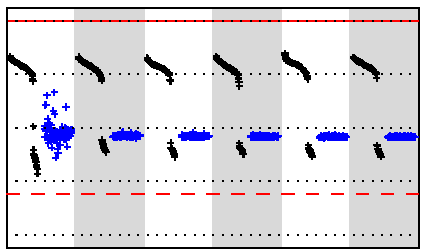
\includegraphics[scale = 0.7]{figs/prioraug/addnoise1.pdf}};
  \node at (0,0) {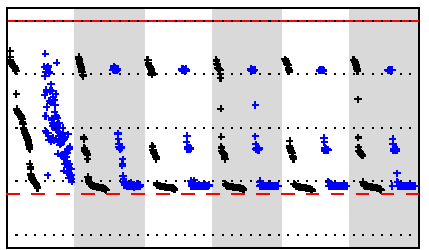
\includegraphics[scale = 0.7]{figs/prioraug/addnoise2.pdf}};
  \node at (-5.2,0) {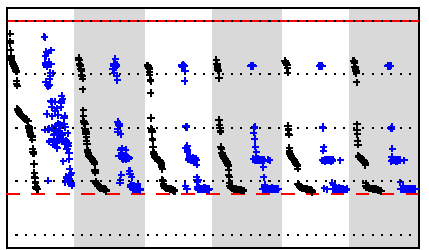
\includegraphics[scale = 0.7]{figs/prioraug/intdiff_heu1.pdf}};
  \node[rotate=90] at (-8.0,0) {Cost};
  \node at (-8.0,1.25) {1.0};
  \node at (-8.0,-1.25) {0.2};
  \node[fill=white,rounded corners] at (-3.5,-1.15) {\scriptsize $\sigma^2 = 0$};
  \node[fill=white,rounded corners] at (1.6,-1.15) {\scriptsize $\sigma^2 = 0.01$};
  \node[fill=white,rounded corners] at (6.85,-1.15) {\scriptsize $\sigma^2 = 0.1$};
\end{tikzpicture}
\label{fig:noisy2}
} 
\subfigure[Reconstruct $\dot\theta$ using the Euler method.]{ % Uncertainty in dtheta
\begin{tikzpicture}
  \node at (5.2,0) {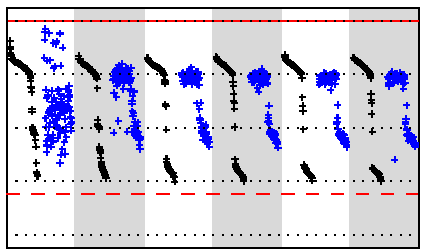
\includegraphics[scale = 0.7]{figs/prioraug/intdiff_eul6.pdf}};
  \node at (0,0) {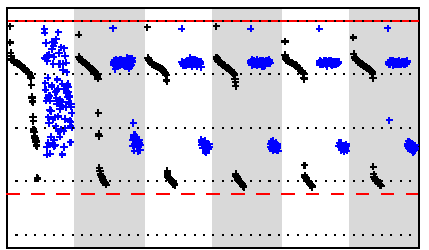
\includegraphics[scale = 0.7]{figs/prioraug/intdiff_eul7.pdf}};
  \node at (-5.2,0) {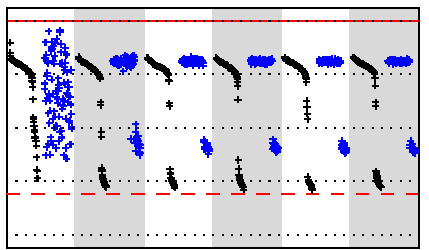
\includegraphics[scale = 0.7]{figs/prioraug/intdiff_eul9.pdf}};
  \node[rotate=90] at (-8.0,0) {Cost};
  \node at (-8.0,1.25) {1.0};
  \node at (-8.0,-1.25) {0.2};
  \node[fill=white,rounded corners] at (-3.5,-1.15) {\scriptsize $\sigma^2 = 0$};
  \node[fill=white,rounded corners] at (1.6,-1.15) {\scriptsize $\sigma^2 = 0.01$};
  \node[fill=white,rounded corners] at (6.85,-1.15) {\scriptsize $\sigma^2 = 0.1$};
\end{tikzpicture}
\label{fig:eul2}
}
\subfigure[Reconstruct $\dot\theta$ using the Heun method.]{ % Uncertainty in dtheta
\begin{tikzpicture}
  \node at (5.2,0) {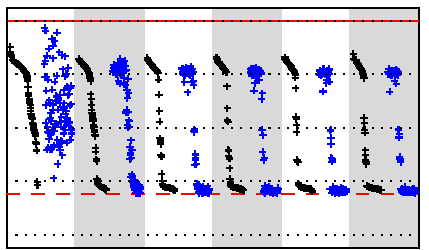
\includegraphics[scale = 0.7]{figs/prioraug/intdiff_heu6.pdf}};
  \node at (0,0) {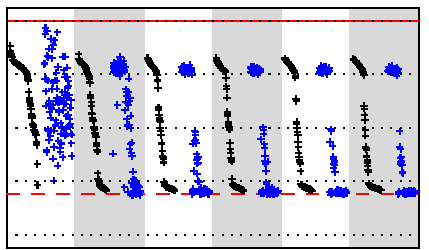
\includegraphics[scale = 0.7]{figs/prioraug/intdiff_heu7.pdf}};
  \node at (-5.2,0) {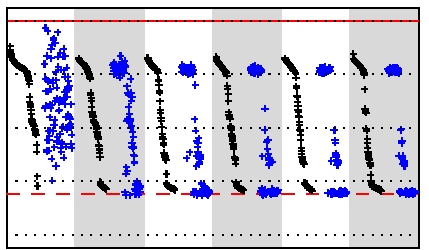
\includegraphics[scale = 0.7]{figs/prioraug/intdiff_heu9.pdf}};
  \node[rotate=90] at (-8.0,0) {Cost};
  \node at (-8.0,1.25) {1.0};
  \node at (-8.0,-1.25) {0.2};
  \node[fill=white,rounded corners] at (-3.5,-1.15) {\scriptsize $\sigma^2 = 0$};
  \node[fill=white,rounded corners] at (1.6,-1.15) {\scriptsize $\sigma^2 = 0.01$};
  \node[fill=white,rounded corners] at (6.85,-1.15) {\scriptsize $\sigma^2 = 0.1$};
\end{tikzpicture}
\label{fig:heu2}
}
\caption{Plots of the distribution of actual costs (black) and the mean predicted cost (blue) for different levels of additive noise $\cN(\bO,\sigma^2\bI)$ on the prediction of $\dot\theta$. The x-axis displays the algorithm iteration and the y-axis shows the cost $J(\bpsi)$. These plots were constructed from 100 Monte Carlo runs with initial training data sets obtained by applying different random torque actions.}
\label{fig:differ}
\end{figure*}
%-------------------------------------------------------------------------------------------------------------------------------------------




\subsubsection{Velocity Reconstruction}
Now consider the use of velocity reconstruction to obtain predictions for $\dot\theta$ based on GP predictions of $\theta$. The Euler and Heun equations in this case are given by
\begin{align}
\dot\theta_k &= \Dt\inv\big(\theta_k - \theta_{k-1}\big) + \epsilon_k
\label{eqn:pen_eulv} \\
\dot\theta_k &= 2\Dt\inv\big(\theta_k - \theta_{k-1} \big) - \dot\theta_{k-1} + \epsilon_k
\label{eqn:pen_heuv}
\end{align}
respectively. We again use noise variances of $\sigma^2=0.01$ and $\sigma^2=0.1$, which correspond, in this case, to standard deviations of $0.1\,$rad$\,$s$\inv$ and $0.316\,$rad$\,$s$\inv$ respectively. Higher order approximations have not actually been considered here since applying them to this problem led to an explosion in the covariance of the predicted state at later timesteps and therefore numerically unstable results. This occurred because the variance in the initial estimates of $\theta$ was quite large, but this uncertainty was then amplified many times since the coefficients of the linear model were relatively large.

The results of the Euler and Heun approximation schemes are given in \Fig{differ}. It is quite clear from these plots that the use of velocity reconstruction leads to much poorer performance than the standard algorithm in all cases. The Euler results shown in \Fig{eul2} fail in almost all the runs and the discrepancy between the predicted and actual costs is large. However, even in the face of such a poor approximation, some of the runs are still able to solve the task.

The effect of additional uncertainty when using a Heun approximation leads to progressively improved results with the best performance achieved when $\sigma^2=0.1$. Increasing noise appears to have the effect of stopping the runs falling into ``weak" local minima such as the two-swing solution and polarises the results into the ``strong" minima of the global optimum and the failure mode.



%-------------------------------------------------------------------------------------------------------------------------------------------
\begin{figure}
\centering \small
\begin{tikzpicture}
  \node at (5.2,0) {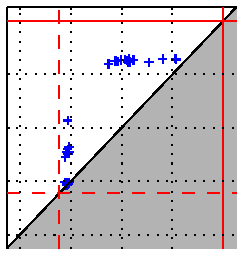
\includegraphics[scale = 1.2]{figs/prioraug/penpred3.pdf}};
  \node at (0,0) {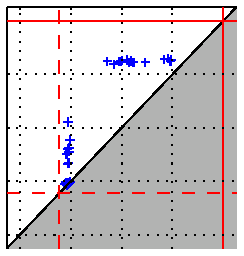
\includegraphics[scale = 1.2]{figs/prioraug/penpred2.pdf}};
  \node at (-5.2,0) {\includegraphics[scale = 1.2]{figs/prioraug/penpred1.pdf}};
  \node[rotate=90] at (-7.95,0) {Predicted Cost};
  \node at (-7.95,2.2) {1.0};   \node at (7.3,-2.85) {1.0};
  \node at (-7.95,-2.15) {0.2};   \node at (-7.3,-2.85) {0.2};
  \node[] at (0,-2.85) {Lowest Predicted Cost using a Globally Optimal Policy};
  \node[fill=white,draw,rounded corners] at (-5.2,-1.9) {$\sigma^2 = 0.10$};
  \node[fill=white,draw,rounded corners] at (0,-1.9) {$\sigma^2 = 0.01$};
  \node[fill=white,draw,rounded corners] at (5.2,-1.9) {$\sigma^2 = 0.00$};
\end{tikzpicture}
\caption{These plots are directly related to the Monte Carlo runs shown in \Fig{heu2} in which a Heun-type method has been used to achieve velocity reconstruction. They show the lowest predicted cost predicted by a given internal model for a globally optimal policy against the policy the algorithm actually converged on using this model. Points appearing in the gray region would indicate that the model was predicting that the globally optimal solution was performing worse than its own solution.}
\label{fig:penpred}
\end{figure}
%-------------------------------------------------------------------------------------------------------------------------------------------



An important question to be raised is why does velocity reconstruction perform so much poorer than position reconstruction. It is evidently not due to the predictive quality of the predictions since for the Heun method these are clearly quite accurate. To investigate this phenomenon a further study was carried out on the Heun Monte Carlo runs shown in \Fig{heu2}. The learned model at the end of the sixth iteration for every run was taken and every policy which achieved the globally optimal solution was evaluated with respect to this model to see whether the policy it had converged on was genuinely optimal with respect to the learned model or whether the algorithm had simply got stuck in a local minimum. The results are shown in \Fig{penpred}. Clearly the problem here is that the use of velocity reconstruction in the pendulum problem produces a problem with stronger local minima than with position reconstruction.

The reason for this strange behaviour could be due to the fact that the dynamics of position variables tend to be slower than the associated velocity. This is because integration in time has a low-pass filtering effect. Therefore, trying to reconstruct the quickly varying dynamics from the slowly varying ones has more potential for erroneous results. 



\subsubsection{Computational Savings}


%-------------------------------------------------------------------------------------------------------------------------------------------
\begin{figure}[t!]
\centering \small
\begin{tikzpicture}
  \node at (0,0) {\includegraphics[scale=1.1]{figs/prioraug/pen_timing.pdf}};
  \node[rotate=90] at (-4.75,0) {CPU time (s)};
  \node[anchor=east] at (-4.3,2.2) {20};   \node[anchor=east] at (-4.3,-2.2) {0};
  \node at (0,-2.6) {Training data set size};
  \node at (-4.2,-2.55) {0};  \node at (4.2,-2.55) {500};
\end{tikzpicture}
\caption{Comparison of CPU time for a single cost function evaluation (with derivatives) for the pendulum. The black line is for the prediction of $\theta$ and $\dot\theta$ using two GPs. The blue line is for the case where one of the states is reconstructed using information back to time $k-1$ and the red line for information back to $k-2$. The x-axis depicts the size of training data set available to the GP.}
\label{fig:pencomps}
\end{figure}
%-------------------------------------------------------------------------------------------------------------------------------------------



One of the major advantages of using prior information in this way is the computational savings in prediction and cost function evaluation. Since we are removing one of the two Gaussian process models (for both position and velocity reconstruction) and replacing it with a linear mapping we expect the computation time to be approximately halved. \Fig{pencomps} shows a plot of the CPU time required to evaluate $J(\bpsi)$ (and its derivatives with respect to policy parameters) against the size of the training data set available to the GP. Below about $n=100$ there is no significant difference between the three except that it costs slightly more to include the delayed states for approximations based on information at time $k-2$. However, beyond $n=200$ the computational savings are significant, with the inclusion of delayed states coming at essentially no extra cost. The trends do indeed show a linear saving in the number of GPs we can replace with linear mappings.









\subsection{Example: Unicycle} \label{sec:unicycle}








%-------------------------------------------------------------------------------------------------------------------------------------------
%\begin{figure}[t]
%\centering
%\subfigure[Robotic unicycle]{
%
\begin{tikzpicture}[]

\begin{scope}[canvas is xz plane at y=-1.5]
  \draw[draw=black,fill=black!10,rounded corners] (2.3,2) rectangle (-2.5,-2);
\end{scope}

% origin is (-2.5,-1.5,2)
\draw[thick,blue,-latex'] (-2.7,-1.5,2) -- (-0.5,-1.5,2);
\draw[thick,blue,-latex'] (-2.5,-1.7,2) -- (-2.5,0.5,2);
\draw[thick,blue,-latex'] (-2.5,-1.5,2.3) -- (-2.5,-1.5,-0.8);

\begin{scope}[canvas is xz plane at y=-0.1]
  \draw[rotate=0,-latex',black, thick] (-2.2,2) arc (0:-320:0.3cm);
\end{scope}
\begin{scope}[canvas is xy plane at z=0.1]
  \draw[rotate=0,-latex',black, thick] (-2.25,-1.5) arc (0:-300:0.25cm);
\end{scope}
\begin{scope}[canvas is yz plane at x=-1.1]
  \draw[rotate=0,-latex',black, thick] (-1.2,2) arc (0:300:0.3cm);
\end{scope}

\begin{scope}[canvas is yx plane at z=-0.05]
  \draw[draw=black,fill=black!30,thick,opacity=0.8] (0,0) circle (1.5cm);
\end{scope}
\begin{scope}[canvas is yx plane at z=0.05]
  \draw[draw=black,fill=black!30,thick,opacity=0.8] (0,0) circle (1.5cm);
  \draw[draw=black,fill=black,thick] (0,0) circle (0.1cm);
  \draw[rotate=45,-latex',red, thick] (1.7,0) arc (0:50:1.7cm);
  \draw[rotate=45,-latex', thick] (0.3,0) arc (0:300:0.3cm);
\end{scope}

\draw[line width = 0.05cm] (0,3,0) -- (0,0,0);
\draw[line width = 0.1cm] (0,3,0) -- (0,1.48,0);

\begin{scope}[canvas is xz plane at y=2.94]
  \draw[draw=black,fill=black!30,thick,opacity=0.8] (0,0) circle (1.5cm);
\end{scope}
\begin{scope}[canvas is xz plane at y=3]
  \draw[draw=black,fill=black!30,thick,opacity=0.8] (0,0) circle (1.5cm);
  \draw[draw=black,fill=black,thick] (0,0) circle (0.1cm);
   \draw[rotate=-5,-latex',red, thick] (1.7,0) arc (0:-50:1.7cm);
   \draw[rotate=0,-latex', thick] (0.4,0) arc (0:-300:0.4cm);
\end{scope}


\node at (-0.4,-1.5,2.8) {{\color{blue}$x$}}; \node at (-0.9,-1.2,1.7) {$\theta$};
\node at (-2.1,-1.5,-0.2) {{\color{blue}$y$}}; \node at (-2.5,-1.0,-0.2) {$\phi$};
\node at (-2.2,0.4,2) {{\color{blue}$z$}}; \node at (-2.9,0.2,2) {$\psi$};

\node at (-0.3,-0.6,0) {$\phi_\text{w}$}; \node at (-0.7,3,0.3) {$\psi_\text{t}$};
\node at (1.9,0.7,0) {\color{red}$u_\text{w}$}; \node at (2.3,3.4,0.5) {\color{red}$u_\text{t}$};


\end{tikzpicture}
%\label{fig:unicycle}
%}
%\hspace{1cm}
%\subfigure[Body centred coordinates]{
%\begin{tikzpicture}
%  \draw[draw=black,fill=black!10,rounded corners] (-3,-3) rectangle (3,3);
%
%  \draw[thick,blue,-latex']  (1,0.9) -- (1,2.5);
%  \draw[thick,blue,-latex']  (0.9,1) -- (2.5,1);
%  \draw[thick,red,fill=red] (1,1) circle (0.06cm);
%  
%  \draw[rotate=50,thick, fill=black!30] (-1.3,0) circle (1cm);
%  \draw[rotate=50,thin] (-1.33,-1) -- (-1.33,1);
%  \draw[rotate=50,thin] (-1.27,-1) -- (-1.27,1);
%  \draw[rotate=50,thick,blue,-latex'] (-1.3,0.1) -- (-1.3,-1.5);
%  \draw[rotate=50,thick,blue,-latex'] (-1.4,0) -- (0.2,0.1);
%  
%  \node at (-0.2,1.3) {\footnotesize origin};
%  \draw[thin,black,-latex']  (0.3,1.3) -- (0.9,1.05);
%  \node at (0.0,-2.0) {\color{blue}$x_c$};
%  \node at (0.2,-0.1) {\color{blue}$y_c$};
%  \node at (2.2,0.75) {\color{blue}$x$};
%  \node at (1.25,2.2) {\color{blue}$y$};
%  
%\end{tikzpicture}
%\label{fig:unicycle2}
%}
%\caption{Robotic unicycle with roll angle $\theta$, pitch angle $\phi$, yaw angle $\psi$, turntable angle $\psi_{\text{t}}$ and wheel angle $\phi_{\text{w}}$. The controlled inputs are the torque applied to the turntable $u_{\text{t}}$ and the torque applied to the wheel $u_{\text{w}}$.}
%\end{figure}
%-------------------------------------------------------------------------------------------------------------------------------------------








\subsubsection{Setup}
The scheme was then tested on a highly nontrivial control problem: balancing a simulated robotic unicycle. The layout of this problem is shown in \Fig{unicycle}. What makes this such a hard problem is that the rolling motion of the unicycle can only be affected indirectly through application of a torque to the turntable on top of the unicycle. The equations of motion for this system were derived by \cite{For09} and can be found in \App{unicycle}, along with a full derivation. 

The state is given by $\bx = [\phi, \dot\phi, \theta, \dot\theta, \psi, \dot\psi, \dot\phi_\te{w}, \dot\psi_\text{t},x_\text{c}, y_\text{c}]^\top \in \RR^{10}$ with pitch angle $\phi$, roll angle $\theta$, yaw angle $\psi$, wheel angle $\phi_\te{w}$, turntable angle $\psi_\te{t}$ and the location of the origin $(x_\te{c},y_\te{c})$ with respect to a body-fixed reference frame. These are depicted in \Fig{unicycle}. We note that the dynamics are clearly independent of $\phi_\te{w}$ and $\psi_\te{t}$ for a wheel and turntable with uniform radial distribution of mass.  The constrained action vector is $\bu = [u_\te{w}, u_\te{t}]^\top \in \RR^2$, where $u_\te{w}$ is the torque applied to the wheel and $u_\te{t}$ is the torque applied to the turntable.

The policy itself was an affine policy $\bu = \bK\bx + \bk$ with gain matrix $\bK$ and offset $\bk$. Note that the distinction between these terms and the covariance matrix of a GP will be clear from the context. The discrete timestep was set to $\Dt = 0.15\,$s. This is a large timestep given the dynamics of the unicycle and therefore makes the task of control relatively hard. However, a long timestep is necessary to ensure the policy learning time is not in the order of weeks.


%-------------------------------------------------------------------------------------------------------------------------------------------
\begin{figure}
\centering
%set the plot display orientation
%synatax: \tdplotsetdisplay{\theta_d}{\phi_d}
\tdplotsetmaincoords{65}{100}

%define polar coordinates for some vector
%TODO: look into using 3d spherical coordinate system
\pgfmathsetmacro{\magW}{4}
\pgfmathsetmacro{\psiW}{-30}
\pgfmathsetmacro{\theW}{10}
\pgfmathsetmacro{\phiW}{15}

%start tikz picture, and use the tdplot_main_coords style to implement the display 
%coordinate transformation provided by 3dplot
\footnotesize
\begin{tikzpicture}[scale=0.95,tdplot_main_coords]

%set up some coordinates ... GET FROM MATLAB
%-----------------------
\coordinate (O) at (1.7321,-1,0);
\coordinate (B) at (2.5,4.3301,0);
\coordinate (Bp) at (4.2321,3.3301,0);
\coordinate (W) at (2.7256,4.1999,1.4772);
\coordinate (Wt) at (3.1767,3.9394,4.4316);
\coordinate (Wtp) at (2.7256,4.1999,4.4316);
\coordinate (Wbp) at (2.7256,4.1999,0);
\coordinate (T) at (2.7969,2.8138,5.7578);
\coordinate (F) at (2.7612,3.5069,3.6175);

%draw figure contents
%--------------------

%draw the main coordinate system axes
\tdplotsetrotatedcoordsorigin{(O)}
\tdplotsetrotatedcoords{0}{0}{0}
\draw[tdplot_rotated_coords,-latex,blue,thick] (0,0,0) -- (1.5,0,0) node[anchor=south east]{$\bi$};
\draw[tdplot_rotated_coords,-latex,blue,thick] (0,0,0) -- (0,1.5,0) node[anchor=south]{$\bj$};
\draw[tdplot_rotated_coords,-latex,blue,thick] (0,0,0) -- (0,0,1.5) node[anchor=south]{$\bk$};
\draw[dashed] (W) -- (Wt);
\draw[dashed] (Wtp) -- (Wbp);
\draw[dashed] (B) -- (W);

\draw[red,-latex] (B) -- (Bp);
\draw[red,-latex] (Bp) -- (O);
\node at (0,0.8,-1.7) {\color{red} $x_\te{c}$};
\node at (0,3.2,-1.4) {\color{red} $y_\te{c}$};
\tdplotsetrotatedcoords{\psiW}{0}{0}
\tdplotsetrotatedcoordsorigin{(Bp)}
\draw[tdplot_rotated_coords,very thin] (-0.35,0,0) -- (-0.35,-0.35,0) -- (0,-0.35,0);


% draw frame
\draw[very thick,black] (W) -- (T);
\tdplotsetrotatedcoords{\psiW}{100}{0}
\tdplotsetrotatedcoordsorigin{(F)}
\draw[tdplot_rotated_coords,fill=black] (0,0,0) circle (0.12);

% draw turntable
\tdplotsetrotatedcoords{\psiW}{\theW}{\phiW}
\tdplotsetrotatedcoordsorigin{(T)}
\draw[tdplot_rotated_coords,very thick,fill=black,fill opacity=0.2] (0,0,0) circle (1.5);
\draw[tdplot_rotated_coords,fill=black] (0,0,0) circle (0.12);
\tdplotdrawarcarrow[tdplot_rotated_coords,red]{(T)}{0.65}{0}{270}{}{}
\tdplotdrawarcarrow[tdplot_rotated_coords,blue]{(T)}{0.4}{0}{270}{}{}
\node at (0,3.25,4.8) {\color{red} $\psi_\te{t}$};
\node at (0,1.7,4.2) {\color{blue} $u_\te{t}$};

% draw wheel
\tdplotsetrotatedcoords{\psiW}{100}{0} % add 90 to j angle
\tdplotsetrotatedcoordsorigin{(W)}
\draw[tdplot_rotated_coords,very thick,fill=black,fill opacity=0.2] (0,0,0) circle (1.5);
\draw[tdplot_rotated_coords,fill=black] (0,0,0) circle (0.12);
\tdplotdrawarcarrow[tdplot_rotated_coords,red]{(W)}{0.6}{0}{270}{}{}
\tdplotdrawarcarrow[tdplot_rotated_coords,blue]{(W)}{0.4}{0}{270}{}{}
\node at (0,4.35,0.5) {\color{red} $\phi_\te{w}$};
\node at (0,3.3,-0.1) {\color{blue} $u_\te{w}$};



% show theta and phi
\tdplotdrawarcarrow[red]{(O)}{0.8}{0}{60}{anchor=north}{\color{red} $\psi$}
\tdplotsetrotatedcoords{\psiW}{190}{-90} % add 180 to j angle
\tdplotsetrotatedcoordsorigin{(W)}
\tdplotdrawarcarrow[tdplot_rotated_coords,red]{(W)}{2.8}{80}{90}{anchor=south}{\color{red} $\theta$}
\tdplotsetrotatedcoords{\psiW}{100}{0} % add 90 to j angle
\tdplotsetrotatedcoordsorigin{(W)}
\tdplotdrawarcarrow[tdplot_rotated_coords,red]{(W)}{2.8}{180}{195}{anchor=south}{\color{red} $\phi$}


\end{tikzpicture}
\caption{The robotic unicycle. The spatial position of the unicycle is defined by the pitch angle $\phi$, roll angle $\theta$, yaw angle $\psi$, wheel angle $\phi_\te{w}$, turntable angle $\psi_\te{t}$ and the body-centred coordinates of the global origin $(x_\te{c},y_\te{c})$. The controlled inputs are the motor torque applied to the wheel $u_\te{w}$ and the motor torque applied to the turntable $u_\te{t}$.}
\label{fig:unicycle}
\end{figure}
%-------------------------------------------------------------------------------------------------------------------------------------------




%-------------------------------------------------------------------------------------------------------------------------------------------
\begin{figure}
\centering \footnotesize
\subfigure[GP models for all states]{ % Uncertainty in theta
\begin{tikzpicture}
  \node at (0,0) {\includegraphics[scale = 0.75]{figs/prioraug/uniplotY1.pdf}};
  \node[rotate=90] at (-3.75,0) {Cost};
  \node at (-3.7,1.6) {1}; \node at (-3.7,-1.7) {0};
\end{tikzpicture}
\label{fig:uni_sta}
}
\subfigure[Reconstruct $\phi, \theta$ and $\psi$ using the Euler method]{ % Uncertainty in theta
\begin{tikzpicture}
  \node at (0,0) {\includegraphics[scale = 0.75]{figs/prioraug/uniplotY2.pdf}};
  \node[rotate=90] at (-3.75,0) {Cost};
  \node at (-3.7,1.6) {1}; \node at (-3.7,-1.7) {0};
\end{tikzpicture}
\label{fig:uni_eul}
}
\subfigure[Reconstruct $\phi, \theta$ and $\psi$ using the Heun method]{ % Uncertainty in theta
\begin{tikzpicture}
  \node at (0,0) {\includegraphics[scale = 0.75]{figs/prioraug/uniplotY3.pdf}};
  \node[rotate=90] at (-3.75,0) {Cost};
  \node at (-3.7,1.6) {1}; \node at (-3.7,-1.7) {0};
\end{tikzpicture}
\label{fig:uni_heu}
}
\subfigure[Reconstruct $\phi, \theta$ and $\psi$ using the Cubic method]{ % Uncertainty in theta
\begin{tikzpicture}
  \node at (0,0) {\includegraphics[scale = 0.75]{figs/prioraug/uniplotY5.pdf}};
  \node[rotate=90] at (-3.75,0) {Cost};
  \node at (-3.7,1.6) {1}; \node at (-3.7,-1.7) {0};
\end{tikzpicture}
\label{fig:uni_fan}
}
\caption{Boxplots depicting the cost $J(\bpsi)$ of applying the learned control policy after a given iteration of the algorithm. These were constructed from 50 Monte Carlo runs with random initial training data sets of around 10$\,$s. The blue box encloses the 25$\tth$ to 75$\tth$ percentile of the data, with the 50$\tth$ percentile shown by the red line.}
\label{fig:uniplots}
\end{figure}
%-------------------------------------------------------------------------------------------------------------------------------------------





The state measurement was corrupted with uncorrelated Gaussian white noise. Realistic values for the standard deviation of the noise on each state are around $0.01\,$rad for the roll angle, $0.03\,$rad for all other angles, $0.03\,$rad$\,$s$\inv$ for the angular velocities and $3\,$cm for the coordinates states. With this level of noise, the learning task is too hard for the algorithm since the Gaussian processes overestimate the noise variance significantly. This is because a standard assumption of GP modelling is that the input training data is noise free. This issue has been addressed by \cite{MR11} who provide a method called Noisy Input Gaussian Processes (NIGP) which takes account of noise on the inputs during training. Using the NIGP method within the learning algorithm, it is able to learn how to balance the unicycle with this level of noise. However, it is unclear at this stage how to combine NIGP with the multiple dynamics models framework. Therefore we consider a problem in which the standard deviation of the noise on measurements of the angles and positions is reduced by a factor of ten.

The control task was to balance the unicycle at the origin $(x_\te{c},y_\te{c}) = (0,0)$ given an initial position drawn from a Gaussian distribution $x_\te{c},y_\te{c} \sim \cN(0,0.01\bI)$, i.e.\ a standard deviation of 10$\,$cm in both $x_\te{c}$ and $y_\te{c}$. We use an inverted-Gaussian stage-cost very similar to one derived by \cite{DHR11}. The stage-cost is of the form
\begin{equation}
c(\bx) = 1 - \exp\Big(-\tfrac{1}{2}d(\bx)^2\Big)
\label{eqn:unicost}
\end{equation}
where $d(\bx)^2$ is the squared distance from the top of the unicycle to the upright position over the origin. In particular this term is given by $d(\bx)^2 = d_x^2 + d_y^2 + d_z^2$ with components
\begin{align*}
d_x &= x_\te{c} - r\sin\phi \\
d_y &= y_\te{c} - (r+r_\te{w})\sin\theta \\
d_z &= (r+r_\te{w}) - (r_\te{w} + r\cos\phi)\cos\theta
\end{align*}
where $r$ is the unicycle frame length and $r_\te{w}$ is the radius of the wheel. The expectation of this stage-cost can be evaluated in exactly the same way as the standard inverted-Gaussian cost by first augmenting the state space with $\sin\phi, \sin\theta, \cos\theta, \cos(\theta+\phi)$ and $\cos(\theta-\phi)$. 
%
We note that the stage-cost we used was tuned slightly in order to penalise the runs in which the unicycle falls over more heavily. Specifically, deviations in the vertical were penalised more than deviations in the horizontal by using $d(\bx)^2 = \tfrac{1}{2}\big(d_x^2 + d_y^2 + (4d_z)^2\big)$. This encodes the fact that falling over is a more serious deviation than being far away horizontally, since this is a recoverable situation.


To initialise the training data set $\cD$, ten trials were carried out in which random torques were applied over each timestep. This resulted in the unicycle falling over so quickly that only about 3-5 data points could be obtained each time.
%
A heuristic that was employed was in terms of the prediction horizon $H$. The aim was to balance the unicycle for around $T = 10\,$s or $H = \big\lceil 10/\Dt \big\rceil$ steps. Now, in order to decrease the offline computation time required the initial horizon was set to $H_1 = \big\lceil 2/\Dt \big\rceil$. This was then increased at each subsequent iteration according to the rule $H_{i+1} = \min\big\{H, \max\{H_i,\lceil 1.5R_i/\Dt \rceil\} \big\}$, where $R_i$ was the time (in seconds) for which the unicycle was able to balance after the $i\tth$ policy optimisation. To decrease computation time further the optimisation algorithm was limited to 60 function evaluations. Again, this figure was chosen through trial and error and general experience of the problem at hand.

The dynamics were learned using independent Gaussian process models with zero mean squared exponential kernels. The GPs were trained to map the current state $\bx_{k-1}$ to the difference $\bx_k-\bx_{k-1}$, again because this is a more appropriate representation for a zero mean prior. In this case the angle variables were not given a sine/cosine representation.
%
Due to the size of the data sets encountered, sparse approximations (based on the FITC method outlined in \Sec{sparse}) were employed when the data sets went above 300 points and utilised a pseudo-training input set of 300 points. This value was again chosen through an experiential and trial and error procedure.



%-------------------------------------------------------------------------------------------------------------------------------------------
\begin{figure}
\centering \small
\begin{tikzpicture}
  \node at (0,0) {\includegraphics[scale=1.1]{figs/prioraug/uni_data.pdf}};
  \node[rotate=90] at (-4.8,0) {Mean size of data set};
  \node[anchor=east] at (-4.4,2.2) {1200};   \node[anchor=east] at (-4.4,-2.2) {0};
  \node at (0,-2.6) {Algorithm Iteration};
  \node at (-4.1,-2.55) {0};  \node at (4.0,-2.55) {20};
\end{tikzpicture}
\caption{Average data set growth corresponding to the Monte Carlo runs shown in \Fig{uni_sta}. All the data sets grew at around the same rate (represented by the black line) with the exception of the Euler method which grew more slowly due to its poorer performance.}
\label{fig:uni_datasize}
\end{figure}
%-------------------------------------------------------------------------------------------------------------------------------------------




\subsubsection{Results}

The results of running the algorithm with various position reconstruction methods are shown in \Fig{uniplots}. No additional additive noise term was applied in these simulations since it was found that no further improvement could be obtained for this problem.

\Fig{uni_sta} shows the cost trajectory of the standard algorithm as the iterations progress. In crude terms it can be seen that most runs have converged on the ``best" solution by the 14$\tth$ or 15$\tth$ iteration. Moving to the Euler approximation shown in \Fig{uni_eul} it is surprising to see that the algorithm can still solve the learning problem but with generally poorer performance than the standard method. The Heun method produces results comparable to that of the standard method but with arguably slightly faster convergence. Further, the number of runs that fail or incur a high cost in the last 5 iterations is much less than is observed when using the standard method.

Finally, interesting results can be observed with use of the Cubic method. This method achieves the fastest convergence to its final solution with almost all the runs completed by the 11$\tth$ iteration, an improvement over all the other methods. However, the stabilising solution it has found is marginally poorer in terms of cost than the others. This can be put down to overconfidence in the predictive power of the method. 
%
We note that using velocity reconstruction led to variance explosion in the state prediction and numerically unstable results for all methods when applied to this problem and therefore learning was impossible.

%TRY 3rd and 4th ORDER APPROXIMATIONS



%-------------------------------------------------------------------------------------------------------------------------------------------
%\begin{figure}[t!]
%\centering \footnotesize
%\begin{tikzpicture}
%  \node at (0,0) {6 PLOTS, };
%\end{tikzpicture}
%\caption{Sample state trajectory of the stablised unicycle. The top plots show the evolution of the roll $\theta$, pitch $\phi$ and yaw $\psi$ from left to right while the lower plots show the $(x_{\text{c}},y_{\text{c}})$ trajectory followed by the applied wheel torque $u_{\text{w}}$ and turntable torque $u_{\text{t}}$.}
%\label{fig:unitraj}
%\end{figure}
%-------------------------------------------------------------------------------------------------------------------------------------------


\subsubsection{Computational Savings}
As mentioned in the pendulum problem, one of the most appealing aspects of including prior information is in terms of computational saving in the policy optimisation stage of the algorithm. For the unicycle this really is the bottleneck in terms of the speed of the algorithm. During the 20 iterations of the algorithm the data set usually gets up to around 1100 points. The average growth of the data sets for the Monte Carlo runs of the standard algorithm, depicted in \Fig{uni_sta}, are shown by the black line in \Fig{uni_datasize}. The same growth was observed when using the Heun and the Cubic method with a slightly slower growth observed when the Euler method was employed (depicted by the red line), due to slower learning. As expected from the use of a sparse approximation the plots appear to be following a linear growth. Using the Euler or Heun methods leads to reduction of around 40\% in computation while use of state information from $k-2$ leads to around a 30\% reduction. These figures indicate a significant time saving since function evaluations take of the order of one minute for the standard method and therefore around one hour is needed for a single policy optimisation consisting of 60 evaluations.





%-------------------------------------------------------------------------------------------------------------------------------------------
\begin{figure}
\centering \small
\begin{tikzpicture}
  \node at (0,0) {\includegraphics[scale=1.1]{figs/prioraug/uni_timing.pdf}};
  \node[rotate=90] at (-4.7,0) {CPU time (s)};
  \node[anchor=east] at (-4.3,2.2) {90};   \node[anchor=east] at (-4.3,-2.2) {20};
  \node at (0,-2.62) {Training data set size};
  \node at (-3.65,-2.55) {100};  \node at (3.65,-2.55) {1200};
\end{tikzpicture}
\caption{Comparison of CPU time for a single cost function evaluation $J(\bpsi)$ (with derivatives)  for the unicycle with $H = \big\lceil 10/\Dt \big\rceil$ and $\Dt = 0.15\,$s. The black line is for prediction of $\theta$ and $\dot\theta$ with GPs. The blue line is for the case where position states are reconstructed using information back to time $k-1$ and the red line for information back to $k-2$. The x-axis depicts the size of training data set available to the GP.}
\label{fig:unicomps}
\end{figure}
%-------------------------------------------------------------------------------------------------------------------------------------------




\section{Reference Tracking}
\label{sec:reffy}



\subsection{Problem Formulation}
An extension of the regulation problem given by \Eq{Jcost} is now considered. In particular, the problem of forcing a linear combination of the system states $\bC\bx^{\bx}$ to track some reference $\br = \bC^{\br}\bx^{\br}$ where $\bx^{\br} \in \RR^{E_r}$ is the underlying reference state. This will be achieved using a parameterised control policy $\bpi$ which has access to a subset of the full reference state $\bx^{\br}_k[\bi]$ where $\bi$ indicates which elements the policy can use. Mathematically, this problem can be posed as
\begin{align}
& \text{minimise} & J(\bpsi) = \EE_{\btau}\Bigg[ & \sum_{k=0}^{H} c\big(\bC\bx^{\bx}_k - \bC^{\br}\bx^{\br}_k,\bu_k\big) \, \bigg| \, p(\bx^{\bx}_0, \bx^{\br}_0) \Bigg]
\label{eqn:reftrack1} \\
&\text{subject to} & \bx^{\bx}_k &= \bff_{\bx}\big(\bx^{\bx}_{k-1},\bu_{k-1}\big) 
\quad \text{where} \quad \bff_{\bx} \sim p\big(\bff_{\bx}|\cD,\hyp\big) & \label{eqn:reftrack2}\\
\nonumber && \bx^{\br}_k &= \bff_{\br}\big(\bx^{\br}_{k-1}\big) \\
\nonumber && \bu_k &= \bpi\big(\bx^{\bx}_k, \bx^{\br}_k[\bi] \big)
\end{align}
where $\btau := [\bx^{\bx}_0; \bx^{\br}_0; \bu_0 \dots \bx^{\bx}_H]$ is a sampled state-action and reference trajectory. The system dynamics evolve according to the function $\bff_\bx$ while the reference signal is governed by the reference generator $\bff_\br$. We note that $\bff_\br$ may be provided by the user or inferred from data in the same way that we infer the system dynamics. 

In the spirit of \cite{BGW90}, the problem in \Eqs{reftrack1}{reftrack2} can be recast as a regulation problem in terms of an augmented state space and dynamics model. First define the augmented state as $\bx := [\bx^{\bx}; \bx^{\br}]$. Next define the augmented dynamical system
\begin{equation*}
\bx_{k} =
\bff(\bx_{k-1}, \bu_{k-1}) = \bmat{
\bff_{\bx}\big(\bx^{\bx}_{k-1},\bu_{k-1}\big) \\
\bff_{\br}\big(\bx^{\br}_{k-1}\big)
}
\end{equation*}
and the stage-cost $c^{\br}\big(\bx,\bu\big) := c\big([\bC, -\bC^{\br}]\bx,\bu\big)$. The recast problem can now be stated as a regulation problem in terms of the augmented state space
\begin{align}
& \text{minimise} & J(\bpsi) = \EE_{\btau}\Bigg[ & \sum_{k=0}^{H} c^{\br}\big(\bx_k ,\bu_k \big)  \, \bigg| \, p(\bx_0) \Bigg]
 \\
&\text{subject to} & \bx_k &= \bff\big(\bx_{k-1},\bu_{k-1}\big) 
\quad \text{where} \quad \bff \sim p\big(\bff|\cD,\hyp\big) & \\
\nonumber && \bu_k &= \bpi\big( \bx_k[\bj] \big)
\end{align}
where $\bj=[\mathbf{1}; \bi]$ is the new indexing vector. This is in exactly the same form as the original regulation problem posed in \Eqs{learn1}{learn2}. Note that if the moments of the stage-cost $c$ are tractable given a Gaussian input $\bx,\bu \sim \cN$ then so will the moments of $c^{\br}$ since the state has simply undergone a linear transformation and therefore remains Gaussian.



%-------------------------------------------------------------------------------------------------------------------------------------------
\begin{figure}[t]
\centering
\tikzstyle{line} = [draw, -latex]
%
\subfigure[Steps]{
\begin{tikzpicture}
	\footnotesize
	\node at (0,0) {\includegraphics[scale=0.7, clip, trim = .1cm 0cm .1cm 0cm]{figs/prioraug/ref_step.pdf}};
	\node at (0.2,-2.65) {time $(k)$}; \node at (-1.8,1.8) {$r_k$};
	\node at (-2.35,2.1) {1}; \node at (-2.35,0) {0};	\node at (-2.4,-2.1) {-1};
	\node at (-2.1,-2.6) {0};
	\node at (2.05,-2.6) {50};
\end{tikzpicture}
\label{fig:linref1}
}
%
\subfigure[Periodic Waves]{
\begin{tikzpicture}
	\footnotesize
	\node at (0,0) {\includegraphics[scale=0.7, clip, trim = .1cm 0cm .1cm 0cm]{figs/prioraug/ref_square.pdf}};
	\node at (0.2,-2.65) {time $(k)$}; \node at (-1.8,1.8) {$r_k$};
	\node at (-2.35,2.1) {1}; \node at (-2.35,0) {0};	\node at (-2.4,-2.1) {-1};
	\node at (-2.1,-2.6) {0};
	\node at (2.05,-2.6) {50};
\end{tikzpicture}
\label{fig:linref2}
}
%
\subfigure[Filtered Noise]{
\begin{tikzpicture}
	\footnotesize
	\node at (0,0) {\includegraphics[scale=0.7, clip, trim = .1cm 0cm .1cm 0cm]{figs/prioraug/ref_noise.pdf}};
	\node at (0.2,-2.65) {time $(k)$}; \node at (-1.8,1.8) {$r_k$};
	\node at (-2.35,2.1) {1}; \node at (-2.35,0) {0};	\node at (-2.4,-2.1) {-1};
	\node at (-2.1,-2.6) {0};
	\node at (2.05,-2.6) {50};
\end{tikzpicture}
\label{fig:linref3}
}
%
\caption{Examples of reference signals generated from the linear system $\bx^{\br}_k = \bA^{\br}\bx^{\br}_{k-1} + \bb^{\br}e_{k-1}$ where $r_k = [1,\bO]\bx^{\br}$. Plots (a)-(c) were generated using $\bA^{\br}_1, \bb^{\br}_1$, $\bA^{\br}_2, \bb^{\br}_2$ and $\bA^{\br}_3, \bb^{\br}_3$ respectively. The means are plotted in thick solid lines, samples shown by dashed lines and the $2\sigma$ confidence region shaded in grey.}
\label{fig:linrefs}
\end{figure}
%-------------------------------------------------------------------------------------------------------------------------------------------



\subsection{Preview Horizon}
An important point to make is that the problem given in \Eqs{reftrack1}{reftrack2} can handle the situation in which the control policy is allowed to anticipate the impending change in reference by having access to some \textit{preview horizon} of the reference signal. In other words $\bu_k$ is allowed to be functionally dependent on $\br_{k+i}$ for $i \in \ZZ_{[0,H_{\te{p}}]}$ and a preview horizon of $H_{\te{p}}$ steps. This situation can be encoded by defining the reference state to consist of future values of $\br$ over the preview horizon window $\bx^{\br}_k = [\br_k; \br_{k+1} \dots \br_{k+H_{\te{p}}}]$. Then defining the reference dynamics to consist of
\begin{equation*}
\bx^{\br}_{k+1} = \bff_{\br}\big( \bx^{\br}_{k} \big) = \bmat{
\big[\bO \;\; \bI\big] \bx^{\br}_{k} \\[0.1cm]
\bff_{r}(\br_{k+H_{\te{p}}})
}
\end{equation*}
the problem is back into the form outlined in the previous section. This reference tracking work was originally proposed in \cite{HRM11}.









\subsection{Reference Dynamics}

When considering what kind of reference dynamics model to use it is worth noting that many standard reference signals can be generated using a simple linear system of equations. Some examples are given in \Fig{linrefs}. These were generated using $\bx^{\br}_k = \bA^{\br}\bx^{\br}_{k-1} + \bb ^{\br}e_{k-1}$ where $r_k = [1,\bO]\bx^{\br}$, $\bx^{\br} \sim \cN$ and $e_k \sim \cN(0,1)$. In particular \Fig{linrefs}(a-c) were generated using 
\begin{align*}
\bA_1^{\br} &= \bmat{\bO & \bI \\ 0 & \big[\bO \;\; 1\big]} \in \RR^{10}, \quad
\bA_2^{\br} = \bmat{\bO & \bI \\ -1 & \bO} \in \RR^{10}, \quad
\bA_3^{\br} = \bmat{a & b \\ 0 & a} \in \RR^{2} 
\end{align*}
and $\bb_1^{\br} = \bb_2^{\br} = \bO$, $\bb_3^{\br} = [0;c]$ respectively, along with an appropriate distribution over the start state $\bx^{\br}_0$. The constants $a,b$ and $c$ were chosen such that $\cov[r_k] \rightarrow \big(\tfrac{1}{2}\big)^2$ as $k \rightarrow \infty$ where $|a| <1$ is necessary for a stable generator.



We note that an advantage of the learning framework is that the reference generating system could also be inferred directly from the data, in the same way that standard dynamics are learned. For example, if the reference signals for a system came from a human operator then a Gaussian process model could be trained to imitate the trajectories the operator is producing and used for offline simulation.









\subsection{Example: Cart-pole}



\subsubsection{Setup}
For illustrative purposes, consider the problem of tracking a moving setpoint using the cart-pole set up in \Fig{cartpole}. The equations of motion and constant values for this system can be found in \App{cart}.
The tracking task is to follow a moving $x$, denoted $r$, position with the pole balanced upright. The initial state of the system is at the origin $\bx_0 = \bO$. The stage-cost is in the same form as the unicycle cost in \Eq{unicost} in which $c(\bx) = 1 - \exp\big(-\tfrac{1}{2}d(\bx)^2\big)$ where $d(\bx)^2$ is the squared distance from the setpoint. The distance, in this case can be decomposed as $d(\bx)^2 = d_x^2 + d_z^2$ where
\begin{align*}
d_x &= (x-r) + \sin\theta \\
d_z &= \cos\theta
\end{align*}
The prediction horizon was set to $T = 5\,$s with a discretisation time of $\delta_t = 0.1\,$s leading to $H = 50$ steps. The trials at each iteration of the algorithm were stopped if the pole fell. The Gaussian process model trained to learn the dynamics was initialised with five trial runs in which random inputs were applied. This led to an overall experience of around 1.5$\,$s. Four independent GPs with squared exponential covariance functions were used to learn the dynamics. Finally, the structure of the policy was linear and pushed through the standard saturation block to satisfy the input constraints.

%-------------------------------------------------------------------------------------------------------------------------------------------
\begin{figure}
\centering
\begin{tikzpicture}[scale=1]
	
	\draw[fill=black!50, black!50, rounded corners] (-1.2,-0.2) rectangle (1.2,0.2); % body
	\draw[fill=black] (0.9,-0.2) circle (.2cm); \draw[fill=black] (-0.9,-0.2) circle (.2cm); % wheels
	\draw[black, line width = 1.2mm, rotate=-30] (0,0) -- (0,3); % pole
	
	\draw[fill=gray, rotate=-30] (0,3) circle (1mm);
	\draw[dashed] (0,-1.2) -- (0,3);
	\draw[dashed, blue] (-2,-0.8) -- (-2,3);
	\draw[rotate=90, -latex] (1,0) arc (0:-30:1cm);
	\draw[fill=gray] (0,0) circle (1mm);
	
	\node[] at (0.3,1.3) {$\theta$};
	\node[] at (1.1,1.0) {$l$};
	
	
	\draw[xshift=0.3cm,rotate=-30,-latex] (0,0) -- (0,2.85); \draw[xshift=0.3cm,rotate=-30,-latex] (0,0) -- (0,-0.15);
	
	\draw[very thick, blue] (-2,2.85) -- (-2,3.15); \draw[very thick, blue] (-1.85,3) -- (-2.15,3);
	\draw[dotted] (-2,3) -- (1.5,2.5981);
	
	\draw[] (-3,-0.4) -- (3,-0.4);
	
	\node[] at (-1.7,-0.8) {\color{blue} $r$};
	\draw[blue] (-3, -0.7) -- (-3,-0.9);
	\draw[blue,-latex] (-3, -0.8) -- (-2,-0.8);
	
	\node[] at (0.3,-1.2) {$x$};
	\draw[] (-3, -1.1) -- (-3,-1.3);
	\draw[-latex] (-3, -1.2) -- (0,-1.2);
	
	\node[] at (2.8,0) {\color{red}$u$};
	\draw[-latex, red, thick] (1.5, 0) -- (2.5,0);

	
\end{tikzpicture}
\caption{Cart-pole setup with position $x$,  pole angle $\theta$, pole length $l$, action force $u$ and lateral location of the setpoint $r$. The setpoint is shown by the blue cross and the Euclidean distance from the tip of the pole to the setpoint is shown by the dotted line. }
\label{fig:cartpole}
\end{figure}
%-------------------------------------------------------------------------------------------------------------------------------------------









%-------------------------------------------------------------------------------------------------------------------------------------------
\begin{figure}
\centering \footnotesize
\subfigure[No preview horizon]{ % Hp = 1
\begin{tikzpicture}
  \node at (0,0) {\includegraphics[scale = 0.75]{figs/prioraug/cartcost1.pdf}};
  \node[rotate=90] at (-3.75,0) {Cost};
  \node at (-3.7,1.35) {1}; \node at (-3.7,-1.4) {0};
\end{tikzpicture}
\label{fig:cart01}
}
\subfigure[Preview horizon $T_{\te{p}} = 0.1\,$s]{ % Hp = 2
\begin{tikzpicture}
  \node at (0,0) {\includegraphics[scale = 0.75]{figs/prioraug/cartcost2.pdf}};
  \node[rotate=90] at (-3.75,0) {Cost};
  \node at (-3.7,1.35) {1}; \node at (-3.7,-1.4) {0};
\end{tikzpicture}
\label{fig:cart02}
}
\subfigure[Preview horizon $T_{\te{p}} = 0.3\,$s]{ % Hp = 4
\begin{tikzpicture}
  \node at (0,0) {\includegraphics[scale = 0.75]{figs/prioraug/cartcost3.pdf}};
  \node[rotate=90] at (-3.75,0) {Cost};
  \node at (-3.7,1.35) {1}; \node at (-3.7,-1.4) {0};
\end{tikzpicture}
\label{fig:cart03}
} 
\subfigure[Preview horizon $T_{\te{p}} = 1.0\,$s]{ % Hp = 10
\begin{tikzpicture}
  \node at (0,0) {\includegraphics[scale = 0.75]{figs/prioraug/cartcost4.pdf}};
  \node[rotate=90] at (-3.75,0) {Cost};
  \node at (-3.7,1.35) {1}; \node at (-3.7,-1.4) {0};
\end{tikzpicture}
\label{fig:cart04}
}
\caption{Cost incurred by the current policy after a given iteration of the algorithm. The policy has access to different preview horizons $T_{\te{p}}$ of the reference. Black crosses show the actual cost incurred while the blue shows the mean predicted cost. }
\label{fig:cartcosts}
\end{figure}
%-------------------------------------------------------------------------------------------------------------------------------------------


%-------------------------------------------------------------------------------------------------------------------------------------------
\begin{figure}
\centering \footnotesize
\subfigure[No preview horizon]{ % Hp = 1
\begin{tikzpicture}
  \node at (0,3) {};
  \node at (0,0) {\includegraphics[scale = 0.75]{figs/prioraug/cart_step1.pdf}};
  \node at (-2.75,1.1) {$x\,$(m)};
  \node at (0,-2.1) {time$\,$(s)};
  \node at (-3.65,-0.75) {0};  \node at (-3.65,0.75) {1};
  \node at (-3.5,-1.8) {0};  \node at (-2.1,-1.8) {1};  \node at (-0.7,-1.8) {2};
  \node at (0.7,-1.8) {3};  \node at (2.1,-1.8) {4};  \node at (3.5,-1.8) {5};
\end{tikzpicture}
}
\subfigure[Preview horizon $T_{\te{p}} = 0.1\,$s]{ % Hp = 2
\begin{tikzpicture}
  \node at (0,0) {\includegraphics[scale = 0.75]{figs/prioraug/cart_step2.pdf}};
  \node at (-2.75,1.1) {$x\,$(m)};
  \node at (0,-2.1) {time$\,$(s)};
  \node at (-3.65,-0.75) {0};  \node at (-3.65,0.75) {1};
  \node at (-3.5,-1.8) {0};  \node at (-2.1,-1.8) {1};  \node at (-0.7,-1.8) {2};
  \node at (0.7,-1.8) {3};  \node at (2.1,-1.8) {4};  \node at (3.5,-1.8) {5};
\end{tikzpicture}
}
\subfigure[Preview horizon $T_{\te{p}} = 0.3\,$s]{ % Hp = 4
\begin{tikzpicture}
  \node at (0,0) {\includegraphics[scale = 0.75]{figs/prioraug/cart_step3.pdf}};
  \node at (-2.75,1.1) {$x\,$(m)};
  \node at (0,-2.1) {time$\,$(s)};
  \node at (-3.65,-0.75) {0};  \node at (-3.65,0.75) {1};
  \node at (-3.5,-1.8) {0};  \node at (-2.1,-1.8) {1};  \node at (-0.7,-1.8) {2};
  \node at (0.7,-1.8) {3};  \node at (2.1,-1.8) {4};  \node at (3.5,-1.8) {5};
\end{tikzpicture}
}
\subfigure[Preview horizon $T_{\te{p}} = 1.0\,$s]{ % Hp = 10
\begin{tikzpicture}
  \node at (0,0) {\includegraphics[scale = 0.75]{figs/prioraug/cart_step4.pdf}};
  \node at (-2.75,1.1) {$x\,$(m)};
  \node at (0,-2.1) {time$\,$(s)};
  \node at (-3.65,-0.75) {0};  \node at (-3.65,0.75) {1};
  \node at (-3.5,-1.8) {0};  \node at (-2.1,-1.8) {1};  \node at (-0.7,-1.8) {2};
  \node at (0.7,-1.8) {3};  \node at (2.1,-1.8) {4};  \node at (3.5,-1.8) {5};
\end{tikzpicture}
}
\caption{Responses of the cart-pole system corresponding to the costs depicted in \Fig{cartcosts} at the sixth iteration. The policy preview horizon $T_{\te{p}}$ was altered between these four sets of runs. The runs show the step responses of 50 runs after the 10th iteration of the algorithm. Red lines show runs in which the pole falls over or can balance but have not learned to track yet.}
\label{fig:cartplots}
\end{figure}
%-------------------------------------------------------------------------------------------------------------------------------------------



\subsubsection{Results}
The first task the cart-pole system was tasked with was to learn a policy to track a unit step change in position $x$ occurring at 1.5$\,$s. The available preview horizon $T_{\te{p}}$ was varied from $0$ to $1\,$s to investigate the effect of allowing the policy to anticipate the change in setpoint. The predicted and actual costs of 50 Monte Carlo runs over 6 algorithm iterations are shown in \Fig{cartcosts}. It is clear that many runs reach their solution after only two iterations while most finish learning after just three. Further note the decrease in cost of the best solution as the preview horizon is increased. This demonstrates that, as we would expect, being able to anticipate the change is beneficial. Note that there is a failure mode that a significant number of the runs end up in. In this mode the pole is balanced at the origin until the change in setpoint then the policy allows it to fall over! There are also a couple of runs that can keep the pole balanced but have not yet learned to track the setpoint.





The actual solutions to which the algorithm converged are given in \Fig{cartplots}. The blue lines correspond to runs that kept the pole upright while the red lines correspond to the failure mode and runs that did not keep the pole balanced. Note that as the preview horizon is increased the benefit of being able to anticipate the change in setpoint is clear. An interesting artefact from the $T_{\te{p}} = 1.0\,$s runs is that there are two optimal solutions, one in which the cartpole moves so that it is in position at the new setpoint when it changes and one in which it is ready to move as the setpoint changes.
%
Another interesting result from using no preview horizon or $T_{\te{p}} = 0.3\,$s can be observed in \Fig{cart01} and (c). In these cases the policy has chosen to ignore the setpoint reference signal and simply regulate to the $x=1\,$m position. This behaviour results from only considering a single setpoint change rather than a distribution of possible changes.



%-------------------------------------------------------------------------------------------------------------------------------------------
\begin{figure}
\centering \footnotesize
\subfigure[No preview horizon]{ % Hp = 1
\begin{tikzpicture}
  \node at (0,0) {\includegraphics[scale = 0.75]{figs/prioraug/cartcost5.pdf}};
  \node[rotate=90] at (-3.75,0) {Cost};
  \node at (-3.7,1.35) {1}; \node at (-3.7,-1.4) {0};
\end{tikzpicture}
\label{fig:cart05}
}
\subfigure[Preview horizon $T_{\te{p}} = 0.1\,$s]{ % Hp = 2
\begin{tikzpicture}
  \node at (0,0) {\includegraphics[scale = 0.75]{figs/prioraug/cartcost6.pdf}};
  \node[rotate=90] at (-3.75,0) {Cost};
  \node at (-3.7,1.35) {1}; \node at (-3.7,-1.4) {0};
\end{tikzpicture}
\label{fig:cart06}
}
\subfigure[Preview horizon $T_{\te{p}} = 0.3\,$s]{ % Hp = 4
\begin{tikzpicture}
  \node at (0,0) {\includegraphics[scale = 0.75]{figs/prioraug/cartcost7.pdf}};
  \node[rotate=90] at (-3.75,0) {Cost};
  \node at (-3.7,1.35) {1}; \node at (-3.7,-1.4) {0};
\end{tikzpicture}
\label{fig:cart07}
} 
\subfigure[Preview horizon $T_{\te{p}} = 1.0\,$s]{ % Hp = 10
\begin{tikzpicture}
  \node at (0,0) {\includegraphics[scale = 0.75]{figs/prioraug/cartcost8.pdf}};
  \node[rotate=90] at (-3.75,0) {Cost};
  \node at (-3.7,1.35) {1}; \node at (-3.7,-1.4) {0};
\end{tikzpicture}
\label{fig:cart08}
}
\caption{Cost incurred by the algorithm by applying the current best policy after a given iteration (given by the x-axis). Black crosses show the actual cost incurred while the blue shows the predicted cost. }
\label{fig:cartcosts2}
\end{figure}
%-------------------------------------------------------------------------------------------------------------------------------------------


We can of course optimise over a distribution over trajectories as shown in \Fig{linrefs}. The next set of simulations was trained using a step change model that changed at the same time as before but the new setpoint was sampled from the distribution $\cN(0,1)$. The results of learning a control policy to achieve this task are shown in \Fig{cartcosts2}. The first thing to note is that the resulting spread in the actual costs as learning proceeds is not emulated in the predicted costs because the predictions are of the average cost that will be incurred. Bearing this in mind, the predictions match up well with the actual performance. We can again see a significant improvement in performance as the preview horizon is increased.

The most notable feature of these results is that we no longer fall into the same failure models that we did when we considered only a deterministic change in setpoint. With the exception of two, all these runs learned how to track a given setpoint. The only runs that failed were the ones that had to track setpoint changes greater than around 2$\,$m. This makes sense since this is the 2$\sigma$ point for the setpoint distribution.




%-------------------------------------------------------------------------------------------------------------------------------------------
\begin{figure}
\centering \footnotesize
\subfigure[Access only to the reference position]{ % Hp = 1
\begin{tikzpicture}
  \node at (0,0) {\includegraphics[scale = 0.75]{figs/prioraug/cartcost9.pdf}};
  \node[rotate=90] at (-3.75,0) {Cost};
  \node at (-3.7,1.35) {1}; \node at (-3.7,-1.4) {0};
\end{tikzpicture}
\label{fig:cart09}
}
\subfigure[Access to the full reference state.]{ % Hp = 2
\begin{tikzpicture}
  \node at (0,0) {\includegraphics[scale = 0.75]{figs/prioraug/cartcost10.pdf}};
  \node[rotate=90] at (-3.75,0) {Cost};
  \node at (-3.7,1.35) {1}; \node at (-3.7,-1.4) {0};
\end{tikzpicture}
\label{fig:cart10}
}
\caption{Cost incurred by the algorithm by applying the current best policy after a given iteration (given by the x-axis). Black crosses show the actual cost incurred while the blue shows the predicted cost. }
\label{fig:cartcosts3}
\end{figure}
%-------------------------------------------------------------------------------------------------------------------------------------------


The final set of simulations we carried out was to track references generated by the second order filter depicted in \Fig{linref3}. In particular, the reference system we considered was given by
\begin{equation*}
\bx^{\br}_{k+1} = \bmat{0.92 & 2.22 \\ 0 & 0.92}\bx^{\br}_{k} + \bmat{0 \\ 0.1}e_k
\end{equation*}
with $\bx^{\br}_0 = \bO$. In the limit of $k\rightarrow \infty$ the standard deviation of the position term saturates to 0.5$\,$m. We first gave the policy access only to the positional term and the results are shown in \Fig{cart09}. Then we gave the policy access to the full reference state and obtained the results in \Fig{cart10}. These results clearly show that the learning procedure has exploited the additional information to obtain much improved tracking performance.






%-------------------------------------------------------------------------------------------------------------------------------------------
\begin{figure}
\centering \footnotesize
\subfigure[Spinning on the spot]{ % Hp = 1
\begin{tikzpicture}
  \node at (-5.3,0) {\includegraphics[scale = 0.7]{figs/prioraug/uni_spin1_1.pdf}};
  \node at (0,0) {\includegraphics[scale = 0.7]{figs/prioraug/uni_spin1_2.pdf}};
  \node at (-10.6,0) {\includegraphics[scale = 0.7]{figs/prioraug/uni_spin1_3.pdf}};
  
  % y coords
  \node at (-7.7,2) {$x_\te{c}$}; \node at (-7.7,1.3) {1}; \node at (-7.7,0) {0}; \node at (-7.7,-1.3) {-1};
  \node at (-2.4,2) {$y_\te{c}$}; \node at (-2.4,1.3) {1}; \node at (-2.4,0) {0}; \node at (-2.4,-1.3) {-1};
  \node at (-13,2) {$y$}; \node at (-13,1.3) {1}; \node at (-13,0) {0}; \node at (-13,-1.3) {-1};
  
  % x coords
  \node at (-7.4,-2.55) {0}; \node at (-5.3,-2.6) {time (s)}; \node at (-3.2,-2.55) {20};
  \node at (-2.1,-2.55) {0}; \node at (0,-2.6) {time (s)}; \node at (2.1,-2.55) {20};
  \node at (-8.6,-2.55) {$x$}; \node at (-11.9,-2.55) {-1}; \node at (-10.6,-2.55) {0}; \node at (-9.3,-2.55) {1};
\end{tikzpicture}
\label{fig:uni01}
}
\subfigure[Spin whilst moving slowly round the circle]{ % Hp = 1
\begin{tikzpicture}
  \node at (-5.3,0) {\includegraphics[scale = 0.7]{figs/prioraug/uni_spin2_1.pdf}};
  \node at (0,0) {\includegraphics[scale = 0.7]{figs/prioraug/uni_spin2_2.pdf}};
  \node at (-10.6,0) {\includegraphics[scale = 0.7]{figs/prioraug/uni_spin2_3.pdf}};
  
  % y coords
  \node at (-7.7,2) {$x_\te{c}$}; \node at (-7.7,1.3) {1}; \node at (-7.7,0) {0}; \node at (-7.7,-1.3) {-1};
  \node at (-2.4,2) {$y_\te{c}$}; \node at (-2.4,1.3) {1}; \node at (-2.4,0) {0}; \node at (-2.4,-1.3) {-1};
  \node at (-13,2) {$y$}; \node at (-13,1.3) {1}; \node at (-13,0) {0}; \node at (-13,-1.3) {-1};
  
  % x coords
  \node at (-7.4,-2.55) {0}; \node at (-5.3,-2.6) {time (s)}; \node at (-3.2,-2.55) {20};
  \node at (-2.1,-2.55) {0}; \node at (0,-2.6) {time (s)}; \node at (2.1,-2.55) {20};
  \node at (-8.6,-2.55) {$x$}; \node at (-11.9,-2.55) {-1}; \node at (-10.6,-2.55) {0}; \node at (-9.3,-2.55) {1};
\end{tikzpicture}
\label{fig:uni02}
}
\subfigure[Spin whilst moving rapidly round the circle]{ % Hp = 2
\begin{tikzpicture}
  \node at (-5.3,0) {\includegraphics[scale = 0.7]{figs/prioraug/uni_spin3_1.pdf}};
  \node at (0,0) {\includegraphics[scale = 0.7]{figs/prioraug/uni_spin3_2.pdf}};
  \node at (-10.6,0) {\includegraphics[scale = 0.7]{figs/prioraug/uni_spin3_3.pdf}};
  
  % y coords
  \node at (-7.7,2) {$x_\te{c}$}; \node at (-7.7,1.3) {1}; \node at (-7.7,0) {0}; \node at (-7.7,-1.3) {-1};
  \node at (-2.4,2) {$y_\te{c}$}; \node at (-2.4,1.3) {1}; \node at (-2.4,0) {0}; \node at (-2.4,-1.3) {-1};
  \node at (-13,2) {$y$}; \node at (-13,1.3) {1}; \node at (-13,0) {0}; \node at (-13,-1.3) {-1};
  
  % x coords
  \node at (-7.4,-2.55) {0}; \node at (-5.3,-2.6) {time (s)}; \node at (-3.2,-2.55) {20};
  \node at (-2.1,-2.55) {0}; \node at (0,-2.6) {time (s)}; \node at (2.1,-2.55) {20};
  \node at (-8.6,-2.55) {$x$}; \node at (-11.9,-2.55) {-1}; \node at (-10.6,-2.55) {0}; \node at (-9.3,-2.55) {1};
\end{tikzpicture}
\label{fig:uni03}
}
\caption{Plots showing the movement of the base of the balanced unicycle as it tracks a spinning setpoint defined in the body-fixed coordinate system $(x_\te{c},y_\te{c})$. The left hand plots show the actual spatial trajectory of the base of the unicycle in blue whilst the red line shows the trajectory of the front of the wheel in order to demonstrate the spinning motion. The other plots show the reference in black and the relevant state of the unicycle in blue.}
\label{fig:uniorbits}
\end{figure}
%-------------------------------------------------------------------------------------------------------------------------------------------





\subsection{Example: Unicycle}
%\subsubsection{Reference Signal}
We now turn our attention back to the unicycle problem of \Sec{unicycle}. We were unsuccessful in getting the unicycle to track specific references in an absolute coordinate system $(x,y)$ however we did succeed in tracking references defined in the body-fixed coordinate system $(x_\te{c},y_\te{c})$ shown in \Fig{unicycle}. Our reasoning for this is that tracking trajectories in the body-fixed coordinate system could be achieved through an infinite number of possible trajectories in an absolute frame of reference. This is because this coordinate system is invariant to rotations around the global origin. Therefore tracking in body-fixed coordinates is less constraining and less challenging than tracking an equivalent fixed trajectory in an absolute frame. This point will be illustrated more clearly with an example.

We tasked the unicycle to stay on the unit circle in the absolute coordinate system $(x,y)$. In order to do this using absolute coordinates we had to define a reference state space system
\begin{equation*}
\bmat{x^\te{r}_k \\ y^\te{r}_k} = \bmat{ \cos\big(\omega_{\te{o}} \Dt\big) & \sin\big(\omega_{\te{o}} \Dt\big) \\ -\sin\big(\omega_{\te{o}} \Dt\big) & \cos\big(\omega_{\te{o}} \Dt\big) }
\bmat{x^\te{r}_{k-1} \\ y^\te{r}_{k-1}}
\end{equation*}
where $\omega_{\te{o}} = 2\pi/T_{\te{o}}$ with orbital period $T_{\te{o}}$ and we set the initial state $(x^\te{r}_0, y^\te{r}_0)=(0,1)$. The algorithm failed to learn this task for multiple values of $T_{\te{o}}$. It would either balance at the origin or follow an orbital trajectory of random radius, which are local minima of the problem. Even when we set $T_{\te{o}}$ to the value of one of these random orbits the algorithm still failed. However, the problem could be posed in a general way using the body-fixed coordinates $(x_{\te{c}},y_\te{c})$ and simply defining a ``setpoint" of $(x^\te{r}_\te{c},y^\te{r}_\te{c}) = (0,1)$. This ``setpoint'' defines all locations of the unicycle for which the origin is 1$\,$m from its right hand side. Under this setup the algorithm could learn this task slightly quicker than the task of balancing.






After this investigation we defined a more exotic set of trajectories using the reference state space system in body-fixed coordinates given by
\begin{equation*}
\bmat{x^\te{r}_{\te{c},k} \\ y^\te{r}_{\te{c},k}} = \bmat{ \cos\big(\omega_{\te{o}} \Dt\big) & \sin\big(\omega_{\te{o}} \Dt\big) \\ -\sin\big(\omega_{\te{o}} \Dt\big) & \cos\big(\omega_{\te{o}} \Dt\big) }
\bmat{x^\te{r}_{\te{c},k-1} \\ y^r_{\te{c},k-1}}
\end{equation*}
If we now set $(x^\te{r}_{\te{c},0},y^\te{r}_{\te{c},0}) = (0,1)$, this tasks the unicycle to stay on the unit circle but to spin around with a period of $T_{\te{o}}$. Three of the solutions the algorithm learned for $T_\te{o} = 5\,$s are shown in \Fig{uniorbits}. These plots clearly show the variety of solutions available to achieve the same task. The policy guiding the unicycle in \Fig{uni01} simply spins it on the spot, whereas the policies shown in (b) and (c) also travel around the unit circle, at varying speeds. We note that very few of the learned control policies could keep tracking beyond 20$\,$s. This issue highlights one of the problems with only training on a relatively short prediction horizon, in this case 10$\,$s. We did not attempt greater prediction horizons because of the increased computation time required to do this.


Finally, through careful selection of reference generator systems we can train the unicycle to track a figure-of-eight trajectory. For example, this can be achieved using the following state space system
\begin{align*}
\bx^\br_+ &= \bmat{ 
\cos\big(2\omega_{\te{o}} \Dt\big) & \sin\big(2\omega_{\te{o}} \Dt\big) & 0 & 0 \\ 
-\sin\big(2\omega_{\te{o}} \Dt\big) & \cos\big(2\omega_{\te{o}} \Dt\big) & 0 & 0 \\
0 & 0 & \cos\big(\omega_{\te{o}} \Dt\big) & \sin\big(\omega_{\te{o}} \Dt\big) \\
0 & 0 & -\sin\big(\omega_{\te{o}} \Dt\big) & \cos\big(\omega_{\te{o}} \Dt\big)}
\bx^\br \\
\bmat{x^\te{r}_{\te{c},k} \\ y^\te{r}_{\te{c},k}} &= \bmat{1 & 0 & 0 & 0 \\ 0 & 0 & 0 & 1} \bx^\br
\end{align*}
with initial reference state $\bx^\br_0 = [0, 1, 0, 1]\T$. With this setup $x^\te{r}_{\te{c}}$ varies as a sine wave while $y^\te{r}_{\te{c}}$ varies as a cosine wave with twice the period. This was clearly a very difficult problem since we were only able to find one training run, from many attempts, that actually managed to learn a policy which achieved the task. The policy learned after 20 iterations of the algorithm was then run for 30$\,$s and the resulting trajectory is shown in \Fig{uniFOE}. Again, we can see the rotational invariance property of the body-fixed coordinate system as the figure-of-eight is not fixed in absolute coordinates. 




%-------------------------------------------------------------------------------------------------------------------------------------------
\begin{figure}
\centering \footnotesize
\begin{tikzpicture}
  \node at (-5.3,0) {\includegraphics[scale = 0.7]{figs/prioraug/uni_foe_1.pdf}};
  \node at (0,0) {\includegraphics[scale = 0.7]{figs/prioraug/uni_foe_2.pdf}};
  \node at (-10.6,0) {\includegraphics[scale = 0.7]{figs/prioraug/uni_foe_3.pdf}};
  
  % y coords
  \node at (-7.7,2) {$x_\te{c}$}; \node at (-7.7,1.15) {1}; \node at (-7.7,0) {0}; \node at (-7.7,-1.15) {-1};
  \node at (-2.4,2) {$y_\te{c}$}; \node at (-2.4,1.15) {1}; \node at (-2.4,0) {0}; \node at (-2.4,-1.15) {-1};
  \node at (-13,2) {$y$}; \node at (-13,1.15) {1}; \node at (-13,0) {0}; \node at (-13,-1.15) {-1};
  
  % x coords
  \node at (-7.4,-2.55) {0}; \node at (-5.3,-2.6) {time (s)}; \node at (-3.2,-2.55) {30};
  \node at (-2.1,-2.55) {0}; \node at (0,-2.6) {time (s)}; \node at (2.1,-2.55) {30};
  \node at (-8.6,-2.55) {$x$}; \node at (-11.75,-2.55) {-1}; \node at (-10.6,-2.55) {0}; \node at (-9.45,-2.55) {1};
\end{tikzpicture}
\caption{Plots showing the movement of the base of the balanced unicycle as it tracks a figure-of-eight in the body-fixed coordinate system $(x_\te{c},y_\te{c})$. The left hand plots show the actual spatial trajectory of the base of the unicycle in red and the unit circle in black. The other plots show the reference trajectory in black and the relevant state of the unicycle in blue.}
\label{fig:uniFOE}
\end{figure}
%-------------------------------------------------------------------------------------------------------------------------------------------






%In this case the unicycle is no longer be asked to regulate to the origin but to track a moving position on the ground. A bit of work must be done first in order to set this problem up correctly. We shall consider orbits in the global coordinate system $(x,y)$ where $x$ lies along $\bi$ and $y$ lies along $\bj$ from \Fig{unicycle}. First, consider the discrete-time state-space equations describing a circular orbit
%\begin{equation*}
%\bmat{x^r_k \\ y^r_k} = \bmat{ \cos\big(\omega_{\te{o}} \Dt\big) & \sin\big(\omega_{\te{o}} \Dt\big) \\ -\sin\big(\omega_{\te{o}} \Dt\big) & \cos\big(\omega_{\te{o}} \Dt\big) }
%\bmat{x^r_{k-1} \\ y^r_{k-1}}
%\end{equation*}
%where $\omega_{\te{o}} = 2\pi/T_{\te{o}}$ and $T_{\te{o}}$ is the period of the orbit in seconds. The radius of the orbit will depend on the initial conditions $x^r_0$ and $y^r_0$. The problem comes in the fact that the unicycle needs to work in a body-centred coordinate system but currently the reference is in an absolute frame. Therefore the following transformation needs to be done before this reference can be passed to the policy
%\begin{equation*}
%\bmat{x^r_{\te{c}k} \\ y^r_{\te{c}k}} = \bmat{ \cos\psi_k & \sin\psi_k \\ -\sin\psi_k & \cos\psi_k }
%\bmat{x^r_{k} \\ y^r_{k}}
%\end{equation*}
%However, this is a nontrivial task since $\psi$, $x^r_{k}$ and $y^r$ will be jointly Gaussian distributed. In this case we can use the framework provided by augmented dynamics to find a solution. Define the intermediate variables $\ba = [\cos\psi, \sin\psi]\T$, $\bb = [x^r\cos\psi, x^r\sin\psi, y^r\cos\psi, y^r\sin\psi]\T$. Now since we can perform moment matching for linear relationships, trigonometric functions and products of jointly Gaussian variables we can find the distribution of $[x^r_{\te{c}k}, y^r_{\te{c}k}]\T$ given the joint distribution over $[\psi, x^r_{k}, y^r_{k}]\T$. This completes the problem setup.



%The algorithm was run with same parameters as before and for 20 iterations and a prediction horizon of 10$\,$s. The task was to learn a policy to track a circular orbit of of varying periods and 1$\,$m radius. 
%
%This was evidently a difficult task since none of the runs actually managed to track the given target at the correct velocity. However, some interesting insight can be gained. The runs that stayed balanced over the whole time tended to settle into an orbit of varying radius but with period always around 6 to 8$\,$s. Even when the reference period was set in this range the tracking task still failed. 



%We concluded that the reason for the failure of this set of experiments is intrinsic to the unicycle dynamics themselves, which render the problem of position tracking almost impossible. Our reasoning is as follows. It was possible to train the unicycle to orbit around the unit circle by defining the body centred setpoint $(x^r_{\te{c}},y^r_{\te{c}}) = (0,1)$ and tasking the unicycle to ``regulate" to this coordinate. It is clear that this defines every point on the unit circle from \Fig{unicycle2}. The only difference between this task and the reference tracking setup is that we were not asking the unicycle to regulate to a specific moving spatial location.






\section{Summary}
Prior knowledge about a dynamical system often comes in the form of known, or approximate, relationships between subsets of the state variables. We have outlined a method for incorporating this prior knowledge into the general framework of probabilistic learning control outlined in the previous chapter. To achieve this we view the system state as evolving according to multiple dynamics models, or sub-dynamics. The key contribution was then in how to propagate the uncertainty in the predictions, which employed the use of a slightly more restrictive assumption of joint Gaussianity than the assumptions made in the previous chapter.

This method found its most obvious use in encoding position-velocity relationships between state variables and in the modelling of higher order Markov systems. However, we demonstrated that it can also be used to tackle problems of reference tracking in which the system is tasked to regulate to a moving setpoint. In addition to this we can allow the policy to have access to a preview horizon of the reference state and therefore allow the algorithm to learn how best to anticipate a change of setpoint.


We were also interested in the question of how the incorporation of such information would affect the learning speed of the algorithm, both computationally and convergence to a good policy, and the propensity for finding good (or bad) local minima in a given problem. This was examined for the pendulum swing-up and unicycle balancing tasks where we included various approximate models for the position-velocity relationships. As expected, we found that a crude model led to poorer results. However, we found that more elaborate models did not necessarily lead to better solutions. We also noticed that although sometimes the propensity for finding poor locally optimal solutions was decreased in many cases, it was amplified in others, in particular when reconstructing velocity from predictions of the position!

Finally, we demonstrated the capability of the framework to learn reference tracking policies on a simulation of a cart and pole. The policy was able to exploit any preview horizon we gave it to help it anticipate the change. We further noted that learning to track a distribution of possible reference signals led to improved learning performance in terms of avoiding poor local minima. Reference tracking was also shown to work on the unicycle when the reference signal was defined in the body-fixed coordinate system rather than absolute coordinates.
\chapter{P\lowercase{riors} O\lowercase{ver} S\lowercase{ampled} S\lowercase{ystems}}

\section{Introduction}
Augmented dynamics provides a flexible way of incorporating useful forms of prior knowledge. However, the most intuitive place to encode such information in a Bayesian framework is directly in the prior distribution over dynamics functions. In fact, augmented dynamics could be viewed as an implication on the covariance matrix or adding additional structure to it. The form of prior knowledge that we address in this chapter is the notion that our discrete-time dynamical system is, in many cases, a sampled continuous-time system. How can we define a prior over discrete-time dynamics that encodes this assumption?

We must first ask, what is the motivation for defining such a prior? What will the likely savings be? In answer to former, we note that it is often the case that the continuous-time dynamics contain some nice structure, for example they can be decomposed as a sum of a linear part, a nonlinear additive part and a general nonlinear part. For example, the pendulum dynamics are made up of a linear and nonlinear part (see \App{pend}) and the cart-pole dynamics consist of a sum of nonlinear combinations of pairs of variables (see \App{cart}). However, this special structure gets lost when we move to the associated discrete-time dynamics. If we were able to encode or learn this underlying structure then our model would be better equipped to generalise into new areas of the state space. In answer to the latter, the likely savings would be that the trained model should have greater marginal likelihood and its predictive performance should be improved with respect to a na\"{\i}ve treatment of the unknown dynamics as a general nonlinear function.

An obvious example of this is, again, time-derivative related states, in which the exact relationship is clear when written in continuous-time but it becomes a complex function of the other (unknown) dynamics, states and actions when dealing in discrete-time. In general any nice structure in the continuous-time dynamics does not translate into the discrete-time domain. It is this problem that we will tackle through the definition of a new class of priors.


%\section{Continuous-Time Implications}
\section{Problem Outline}
In this section we shall address sampled continuous-time systems. These are discrete-time systems which are obtained by sampling some underlying continuous-time system given by
\begin{equation}
\dot\bx_t = \bff(\bx_t, \bu_t)
\label{eqn:conttime}
\end{equation}
where $t \in \RR$. We shall restrict ourselves, as before,  to the consideration of stationary dynamics where $\bff$ is only dependent on $t$ through $\bx$ and $\bu$.  
%
Now assume that $\bff$ has been drawn from some Gaussian process prior $\bff\sim\mathcal{GP}(\bmm, \bK)$. Or in other words
%
\begin{align*}
\bmm(\bz_t) &= \EE_{\bff}\big[\bff(\bz_t)\big] \\
\bK(\bz_t, \tbz_\tau) &= \cov_{\bff}\big[\bff(\bz_t),\bff(\tbz_\tau)\big]
\end{align*}
%
remembering that $\bz := [\bx;\bu]$. This GP prior can encode prior knowledge we have regarding the continuous-time dynamics e.g.\ invariances, linear relationships and additive nonlinear relationships. We are interested in evaluating the associated prior over a sampled version of the dynamics $\bffs\sim\mathcal{GP}(\bmm_\Delta, \bK_\Delta)$ where
%
\begin{align*}
\bmmD(\bz_t) &= \EE_{\bff}\big[\bffs(\bz_t)\big] \\
\bKD(\bz_t,\tbz_\tau) &= \cov_{\bff}\big[\bffs(\bz_t),\bffs(\tbz_\tau)\big]
\end{align*}
%
Note that the expectation and covariance are still taken with respect to the continuous-time dynamics. Now the actual relationship between continuous and the sampled functions is
\begin{align}
\bx_{t+\Dt} &= \bffs(\bx_t,\bu_t) := \bx_t + \int_{t}^{t+\Dt} \!\!\!\!\! \bff(\bx_\tau,\bu_\tau) \dd \tau
\label{eqn:cont-sample}
\end{align}
with sample time $\Dt$. We want to find the relationship between the continuous-time mean and covariance functions ($\bmm,\bK$) and the associated sampled functions ($\bmm_\Delta, \bK_\Delta$). Inevitably we shall have to be satisfied with an approximation since this integral is in general analytically intractable (with the notable exception of linear systems).

In addition, it would be useful to evaluate the posterior GP when we are given non-uniformly sampled data $\cD = \{\bZ,\bY\}$
\begin{align}
\bZ &= \bmat{ \bx_{t_1}\T & \bu_{t_1}\T \\ \vdots & \vdots \\ \bx_{t_n}\T & \bu_{t_n}\T} \in \RR^{n \times D} &\text{and}
&& \bY &= \bmat{ \bx_{t_1+\delta_{1}}\T \\ \vdots \\ \bx_{t_n+\delta_n}\T } \in \RR^{n\times E} \label{eqn:cD}
\end{align}
where the $\delta_i$ can be different. Finally, in order to incorporate it into the predictive framework, moment matching must be possible. We now consider a novel solution to this problem using an approximation based on numerical integration techniques.




% --------------------------------------------------------------------------------------
\begin{table}
\renewcommand{\arraystretch}{1.25}
\begin{center}
\small
\begin{tabular}{ c | ccccc }
\toprule[1.5pt] 
& {\bf Euler } & {\bf Midpoint } & {\bf Heun } & {\bf Kutta } & {\bf RK4 }  \\
\cline{1-6}\\[-2.5ex]
$a_{ip}$
& $\bmat{0}$
& $\bmat{0 & 0 \\ \tfrac{1}{2} & 0}$ 
& $\bmat{0 & 0 \\ 1 & 0}$
& $\bmat{0 & 0 & 0 \\ \tfrac{1}{2} & 0 & 0 \\ -1 & 2 & 0}$
& $\bmat{0 & 0 & 0 & 0 \\  \tfrac{1}{2} & 0 & 0 & 0 \\ 0 & \tfrac{1}{2} & 0 & 0 \\ 0 & 0 & 1 & 0}$ \\[6ex]
$b_{i}$
& $\bmat{1}$
& $\bmat{0 & 1}$ 
& $\bmat{\tfrac{1}{2} & \tfrac{1}{2}}$ 
& $\bmat{\tfrac{1}{6} & \tfrac{2}{3} & \tfrac{1}{6}}$ 
& $\bmat{\tfrac{1}{6} & \tfrac{1}{3} & \tfrac{1}{3} & \tfrac{1}{6}}$  \\[1ex]
\bottomrule[1.5pt]
\end{tabular}
\end{center}
\caption{Settings of $a_{ip}$ and $b_i$ for some common Runge-Kutta methods.}
\label{tab:RKmeths}
\end{table}
% --------------------------------------------------------------------------------------



\section{Numerical Integration}
\subsection{Taylor-Series Expansion}
For clarity of presentation we shall restrict our attention to the autonomous case in which $\dot\bx_t = \bff(\bx_t)$. The full non-autonomous case is addressed in \Sec{nonaut}. One way of dealing with the intractable integral in \Eq{cont-sample} is by expanding out the dynamics function according to its Taylor-series. A first order expansion would yield
\begin{align*}
\bff(\bx_{t+\tau}) &\approx \bff(\bx_t) \;+\; 
\tau \diff{\bff(\bx_{\tilde\tau})}{\tilde\tau}\bigg|_{\tilde\tau=t}  \\[0.1cm]
%
&=  \bff(\bx_t) \;+\; 
\tau \bff_\bx(\bx_t)  \dot\bx_t  \\
&=  \bff(\bx_t) \;+\; 
\tau \bff_\bx(\bx_t) \bff(\bx_t) 
\end{align*}
where $\bff_\bx(\bx_t) := \frac{\dd \bff(\bx)}{\dd \bx}\big|_{\bx=\bx_t} \in \RR^{E\times E}$. The relationship given by \Eq{cont-sample} can then be rewritten as
\begin{equation}
\bffs(\bx_t) \approx \bx_t + 
\Dt \bff(\bx_t) + \tfrac{1}{2}\Dt^2 \bff_\bx(\bx_t) \bff(\bx_t)
\label{eqn:intdt}
\end{equation}
Therefore the approximate relationships between ($\bmm_{\Delta}, \bK_{\Delta}$) and ($\bmm, \bK$) can be characterised by
\begin{align*}
\bmm_{\Delta}(\bx_t) &\approx \bx_t + 
\EE_\bff\big[\Dt \bff(\bx_t) + \tfrac{1}{2}\Dt^2 \bff_\bx(\bx_t) \bff(\bx_t)\big] \\[0.1cm]
%
\bK_{\Delta}(\bx_t,\tbx_\tau) &\approx 
\cov_\bff\big[\Dt \bff(\bx_t) +  \tfrac{1}{2}\Dt^2 \bff_\bx(\bx_t) \bff(\bx_t),\;
\delta_{\tau} \bff(\tbx_\tau) +  \tfrac{1}{2}\delta_{\tau}^2 \bff_\bx(\tbx_\tau) \bff(\tbx_\tau)\big]
\end{align*}
Note that $\Dt$ need not be the same as $\delta_\tau$. There is an issue of prohibitive algebraic complexity, even for this simple approximation. It would involve the calculation of high order moments such as $\cov_\bff\big[\bff_\bx(\bx_t) \bff(\bx_t), \;\bff_\bx(\tbx_\tau) \bff(\tbx_\tau) \big]$ in which it is not clear how this relates to the functions $\bmm$ and $\bK$. Therefore we turn our attention to a widely used and iterative form of numerical integration, the Runge-Kutta (RK) family of methods.





\subsection{Runge-Kutta Methods}
Runge-Kutta methods consist of a simple set of iterative equations which calculate the Taylor-series approximation exactly for a given order $S$. These can be written in the general form
\begin{align}
\bffs(\bx_t) &= \bx_t + \Dt \sum_{i=1}^{S}b_i \bff( \bp_i) \label{eqn:RK1}
\\
\bp_i &= \bx_t + \Dt \sum_{p=1}^{i-1} a_{ip} \bff( \bp_p ) \label{eqn:RK2}
\end{align}
for stationary dynamics where $a_{ip}$, $b_i$ and $c_i$ are the constants associated with a given method. These constants are subject to the constraint $\sum_i b_i = 1$ if the method is to be consistent. By way of example, the constants for some common Runge-Kutta methods are given in \Tab{RKmeths}. These are Euler's method, the Midpoint method, Heun's method, Kutta's method and the popular Runge-Kutta fourth order method (RK4). 
%We shall refer to the family of second order methods as ``RK2", which encompasses both the Midpoint and Heun methods.
Now under this class of methods for numerical integration we can form a tractable approximate relationship from continuous-time to discrete-time as we shall now describe. 




\section{Priors Over Sampled Continuous-Time Systems} \label{sec:priorovercont}


\subsection{Illustrative Examples}
In order to find the relationship between $\bmm$, $\bK$ and $\bmm_{\Delta}$, $\bK_{\Delta}$ consider an approximation using a Runge-Kutta method, given by \Eqs{RK1}{RK2}.
It is useful at this stage to work through the procedure for a couple of simple methods before moving onto the general framework. If we consider the simplest case of an Euler scheme we have the relationship
\begin{align*}
\bffs(\bx) &= \bx + \Dt \bff(\bx)
\end{align*}
It is clear that in this instance the sampled mean and covariance function are simply scalings and translations of the continuous mean and covariance functions
\begin{align*}
\bmm_\Delta(\bx) &= \EE_{\bff}[\bffs(\bx)] &  \bK_\Delta(\bx,\tbx) &= \cov_\bff[\bffs(\bx),\bffs(\tbx)] \\
&= \bx + \Dt \EE_\bff[\bff(\bx)]             & &= \Dt\delta_\tau \cov_{\bff}[\bff(\bx),\bff(\tbx)] \\
&= \bx + \Dt \bmm(\bx)                     & &= \Dt\delta_\tau \bK(\bx,\tbx) 
\end{align*}
Therefore, since the core structure of the sampled mean and covariance remain the same as in continuous-time, we can conclude that \textit{applying the Euler method does not provide any improvement over the standard method in terms of exploiting continuous-time structure}. Now we will work through the Midpoint method, given by
\begin{align*}
\bffs(\bx) &= \bx + \Dt \bff\big(\bx + \tfrac{1}{2}\Dt \bff(\bx)\big)
\end{align*}
First summarise the term in brackets as $\bp = \bx + \tfrac{1}{2}\Dt \bff(\bx)$. It is clear that this will be Gaussian distributed with mean $\bx + \tfrac{1}{2}\Dt \bmm(\bx)$ and covariance $\tfrac{1}{4}\Dt^2 \bK(\bx,\bx)$ for a given value of $\bx$.
%
Therefore the sampled mean and covariance functions will be given by
\begin{align*}
\bmm_\Delta(\bx) &= \bx + \Dt \EE_{\bff,\bp}\big[\bff(\bp)\big]  &  
\bK_\Delta(\bx,\tbx) &= \Dt\delta_\tau\cov_{\bff,\bp,\tbp}\big[\bff(\bp),\bff(\tbp)\big] \\
&= \bx + \Dt \EE_{\bp}[\bmm(\bp)] &
&= \Dt\delta_\tau\Big( \EE_{\bp,\tbp}\big[\bK(\bp,\tbp) + \bmm(\bp)\bmm(\tbp)\T\big] \\[-0.1cm]
&&&\qquad\qquad\qquad\qquad\qquad
-\EE_{\bp}[\bmm(\bp)]\EE_{\tbp}[\bmm(\tbp)]\T \Big)
\end{align*}
where integrals over the continuous mean and covariance function with respect to the random variables $\bp$ and $\tbp$ are required. This is a very similar requirement to the moment matching condition, although now we require cross-covariance terms. The effect of this structural change to the prior will be discussed in \Sec{intuition}. We shall now work through how to do this for a general Runge-Kutta method.


\subsection{General Framework}
Let us employ the assumption that $\bff(\bp_i)$ and $\bff(\tbp_j)$ for $i,j \in \ZZ_{[1,S]}$ are jointly Gaussian distributed given $\bp_i,\tbp_j \sim \cN$. Under this assumption we can apply the process outlined in the illustrative examples for arbitrary orders of the Runge-Kutta method. Note that an implication of this assumption is that $\bp_i$ and $\bp_j$ will be jointly Gaussian since they are related linearly through \Eq{RK2}. In this case we can write
\begin{align}
\bmm_{\Delta}(\bx) &= \bx + \Dt \sum_{i=1}^{S} b_i \,\EE\big[\bff(\bp_i)\big]  \label{eqn:Mdelta} \\
%
\bK_{\Delta}(\bx,\tilde\bx) &= \Dt \delta_{\tau} \sum_{i=1}^{S} \sum_{j=1}^S b_ib_j \,
\cov\big[\bff(\bp_i), \bff(\tbp_j) \big] \label{eqn:Vdelta}
\end{align}
where $\bp_i$ and $\tbp_j$ denote $\bp_i(\bx_t)$ and $\bp_j(\tbx_\tau)$ respectively and the integrals are taken with respect to the random vectors $\bp_i, \tbp_j$ and function $\bff$. 
Similarly for \Eq{RK2} we can use the following iterative rule
\begin{align}
\EE[\bp_i] &= \bx + \Dt \sum_{p=1}^{i-1} a_{ip}\, \EE\big[\bff(\bp_p)\big]
\label{eqn:piter1} \\
\cov[\bp_i, \tbp_j] &= \Dt \delta_{\tau} \sum_{p=1}^{i-1} \sum_{q=1}^{j-1} a_{ip} a_{jq}\, \cov\big[\bff(\bp_p), \bff(\tbp_q)\big]
\label{eqn:piter2}
\end{align}
Now all that remains is to evaluate the expectation $\EE\big[\bff(\bp_i)\big]$ and covariance $\cov\big[\bff(\bp_i), \bff(\tbp_j) \big]$ in these equations. These can be calculated using a moment matching type procedure similar to that of \Sec{multistep}
\begin{align}
\EE_{\bp,\bff}\big[\bff(\bp)\big] 
&= \EE_{\bp}\big[\bmm(\bp)\big] \label{eqn:Efc} \\
\cov_{\bp,\tbp,\bff}\big[\bff(\bp), \bff(\tbp)\big]
&= \EE_{\bp,\tbp}\big[\bK(\bp,\tbp) + \bmm(\bp)\bmm(\tbp)\T\big]
- \EE_{\bp}\big[\bmm(\bp)\big] \EE_{\tbp}\big[\bmm(\tbp)\big]\T \label{eqn:Cfc}
\end{align}
where the integrals are again taken with respect to the random vectors $\bp_i, \tbp_j$ and function $\bff$. The difference between this and the procedure in \Sec{multistep} is that a cross covariance is required in this calculation rather than the covariance of a single random vector $\cov\big[\bff(\bp_i)\big]$. However, any mean and covariance function which satisfies the moment matching criteria will also satisfy this criterion and can be used in this context.

The full structural definition of a new set of priors over sampled autonomous continuous-time dynamical systems is given by \Eqs{Mdelta}{Cfc}. The more general non-autonomous case is discussed in the following section and some examples of kernels for which \Eqs{Efc}{Cfc} can be evaluated are given in \Sec{usekernels}.














\subsection{Non-Autonomous Case} \label{sec:nonaut}
Obviously from a control perspective we are most interested in dealing with systems with external inputs $\bu$. So how do we deal with them in this framework? First imagine that our $\bp$ values are expanded to include a state and an action part $\bp = [\bpx{}; \bpu{}]$. If the action is applied independently of the state over the timestep, for example if it is zero-order hold, first order hold or some other time-dependent function then \Eqs{piter1}{piter2} can be extended trivially as
\begin{align}
\EE[\bp_i] &= \bmat{ \bx \\ \bu + \bee(c_i, \bu) } + \Dt \sum_{p=1}^{i-1} a_{ip}\, 
\bmat{ \EE\big[\bff(\bp_p)\big] \\ \bO } 
\label{eqn:nonaut1} \\
\cov[\bp_i, \tbp_j] &= \Dt \delta_{\tau} \sum_{p=1}^{i-1} \sum_{q=1}^{j-1} a_{ip} a_{jq}\,
\bmat{ \cov\big[\bff(\bp_p), \bff(\tbp_q)\big] & \bO \\ \bO & \bO }
\label{eqn:nonaut2}
\end{align}
where $c_i \in \RR_{[0,1]}$ and $\bee(c_i, \bu) = \bO$ for a zero-order hold scheme and $\bee(c_i, \bu) = c_i(\bu_+ \! - \bu)$, where $\bu_+$ is the action at the following timestep, for a first-order hold scheme. Note that this is not the same as saying that there is not a feedback policy acting on the system, but rather that the policy does not make any state-dependent changes within the sampling window.

Things get a little more complicated if we consider that the action is governed by some policy $\bu = \bpi(\bx)$ over the time interval.  In this case we have the following relationships
\begin{align*}
\EE[\bp_i] &= \bmat{ \bx \\ \bO} + \Dt \sum_{p=1}^{i-1} a_{ip}\, 
\bmat{ \EE\big[\bff(\bp_p)\big] \\[0.1cm] \EE\big[\bpi(\bp_p)\big] }  \\
\cov[\bp_i, \tbp_j] &= \Dt \delta_{\tau} \sum_{p=1}^{i-1} \sum_{q=1}^{j-1} a_{ip} a_{jq}\,
\bmat{ 
\cov\big[\bff(\bp_p), \bff(\tbp_q)\big] & \cov\big[\bff(\bp_p), \bpi(\tbp_q)\big] \\[0.1cm] 
\cov\big[\bpi(\bp_p), \bff(\tbp_q)\big] & \cov\big[\bpi(\bp_p), \bpi(\tbp_q)\big] }
\end{align*}
where the mean $\EE\big[\bpi(\bp_p)\big]$ and covariance $\cov\big[\bpi(\bp_p), \bpi(\tbp_q)\big]$ are dependent only on the form of the function $\bpi$. However, there is no general way of calculating the cross covariance term $\cov\big[\bff(\bp_p), \bpi(\tbp_q)\big]$. Fortunately in this case we can appeal to the results of \Sec{augmentedDYN} to obtain the approximate relationship
\begin{align*}
\cov\big[\bff(\bp_p), \bpi(\tbp_q)\big] &= 
\cov\big[\bff(\bp_p), [\bp_p;\tbp_q] \big]
\cov\big[[\bp_p;\tbp_q]\big]\inv
\cov\big[[\bp_p;\tbp_q], \bpi(\tbp_q)\big]
\end{align*}
to provide a complete framework.





\subsection{Priors Over Useful Function Classes} \label{sec:usekernels}
\subsubsection{Class of Functions}
First we must consider the kind of structure we would like to draw out when we carry out this inference. We believe that a useful space of continuous-time functions to search over is the sum of a full nonlinear part, an additive part and a linear part
\begin{align}
\bff(\bz) &=  \bff_{\text{full}}(\bz) + \bff_{\te{add}}(\bz)  + \bff_{\text{lin}}(\bz)\\
\nonumber &= \bff_{\text{full}}(\bz) + \sum_{i=1}^D\bff_{\te{add},i}\big(z[i]\big) + \bA\bz
\end{align}
If we make the unrestrictive assumption that $\bff_{\text{full}}(\bz)$, $\bff_{\text{add}}(\bz)$ and $\bff_{\text{lin}}(\bz)$ are each drawn from independent Gaussian process priors then the GP parameterising the distribution over the whole function $\bff$ consists simply of the sum of the individual mean and covariance functions
\begin{equation*}
\bff \sim \mathcal{GP}\Big(\bmm_{\text{full}} + \bmm_{\text{add}} + \bmm_{\text{lin}},
\bK_{\text{full}} + \bK_{\text{add}} + \bK_{\text{lin}} \Big)
\end{equation*}
We shall only consider a useful subset of this prior given by $\mathcal{GP}\big(\bmm_{\text{lin}}, \bK_{\text{full}} + \bK_{\te{add}} \big)$.  MATLAB code to evaluate this prior is provided in \App{codePrior} and the function \texttt{prior.m}. We will now evaluate \Eqs{Efc}{Cfc} for each term in this prior.




\subsubsection{Full Nonlinear Part}
A general prior over the space of smooth nonlinear functions is the zero mean, squared exponential covariance prior. In this instance \Eqs{Efc}{Cfc} become 
\begin{align*}
\EE_{\bp,\bff}\big[\bff(\bp)\big] 
&= \mathbf{0} \\
\cov_{\bp,\tbp,\bff}\big[\bff(\bp), \bff(\tbp)\big]
&= \EE_{\bp,\tbp}\big[\bK(\bp,\tbp)\big]
\end{align*}
Again, we shall restrict our attention to a diagonal kernel. The $(a,a)\tth$ element of the expectation of the prior covariance $K[a,a]$ with respect to a joint distribution over the two random variables $\hbp := [\bp;\tbp] \sim \cN(\bm,\bS)$ is then given by
\begin{align}
\nonumber \cov_{\bp,\tbp,\bff}\big[f[a](\bp), f[a](\tbp)\big]
&= \int K[a,a](\hbp) \cN(\hbp | \bm, \bS) \dd \hbp \\
\nonumber &= \int  \alpha_{a}^2 \exp\Big(-\half(\bp - \tbp)\T\bLa_{a}^{-1}(\bp - \tbp) \Big)
\cN(\hbp | \bm, \bS) \dd \hbp \\
\nonumber &= \int  \alpha_{a}^2 \exp\Bigg(-\half\hbp\T 
\underbrace{ \bmat{\bI \\ -\bI}\bLa_{a}^{-1} \bmat{\bI & -\bI} }_{\hat\bLa_{a}^{-1}}
\hbp \Bigg) \cN(\hbp | \bm, \bS) \dd \hbp \\[-0.1cm]
\nonumber &=  \alpha_{a}^2 (2\pi)^{\sfrac{D}{2}}|\hat\bLa_{a}|^{-\sha} \int \cN(\hbp|\bO, \hat\bLa_{a}) \cN(\hbp | \bm, \bS) \dd \hbp \\
&=  \alpha_{a}^2 \big|\bS\hat\bLa_{a}\inv + \bI\big|^{-\sha} 
\exp\Big( - \half \bm\T (\hat\bLa_{a} + \bS)\inv \bm \Big)
\label{eqn:SEprop}
\end{align}
Now since $\hat\bLa_{a}\inv$ is not full rank it should not appear in its un-inverted form. However, we can simply rewrite the term $(\hat\bLa_{a} + \bS)\inv$ as $\hat\bLa_{a}^{-\sha}  \big(\hat\bLa_{a}^{-\sha} \bS\hat\bLa_{a}^{-\sha}  + \bI\big)\inv\hat\bLa_{a}^{-\sha} $ where $\hat\bLa_{a}^{-\sha} = \tfrac{1}{\sqrt{2}}[\bI,-\bI]\T\bLa_{a}^{-\sha}[\bI,-\bI]$ for a numerically stable and symmetric calculation.



\subsubsection{Additive Nonlinear Part}
As shown in \Sec{multistep} the propagation of uncertainty equations for the general additive SE kernel is closely related to the equations for the standard kernel. The same is clearly true in this instance.



\subsubsection{Linear Part}
We have already shown that a distribution of linear systems can be parameterised as
\begin{align*}
\bmm(\bp) &= (\bI \otimes \bp\T)\bet \\
\bK(\bp,\tbp) &= (\bI \otimes \bp\T) \bOm (\bI \otimes \tbp)
\end{align*}
It is clear by looking at the standard moment matching equations provided in \Eqs{linMU}{linSIG} that the expressions for \Eqs{Efc}{Cfc} are very closely related. In fact they are given by
\begin{align*}
\EE_{\bp,\bff}\big[\bff(\bp)\big]  
&= (\bI_E \otimes \mathbf{1}_D\T) \Big( (\mathbf{1}_E  \otimes \bm) \circ \bet \Big) \\
%
\cov_{\bp,\tbp,\bff}\big[\bff(\bp), \bff(\tbp)\big] &= 
 (\bI_E \otimes \mathbf{1}_D\T)
\Big(\big(  \mathbf{1}_{E\times E}\otimes  (\bar\bS + \bm\tilde\bm\T) \big) \big(\bOm+\bet\bet\T\big) \Big) 
 (\bI_E \otimes \mathbf{1}_D) \\[-0.1cm]
& \qquad\qquad\qquad\qquad\qquad\qquad\qquad\qquad\qquad\qquad
- \EE_{\bp,\bff}\big[\bff(\bp)\big] \EE_{\tbp,\bff}\big[\bff(\tbp)\big] \T
\end{align*}
where $\bm = \EE[\bp], \tilde\bm = \EE[\tbp]$ and $\bar\bS = \cov[\bp,\tbp]$. Of course we only require the expression for the mean since we restrict our attention to the prior $\mathcal{GP}\big(\bmm_{\text{lin}}, \bK_{\text{add}} + \bK_{\te{full}} \big)$.







\subsection{Structural Implications on the Prior} \label{sec:intuition}
In order to gain a little more insight into the way the structure of the continuous-time prior is actually altered through this process we shall return to the illustrative example of the midpoint method. We shall consider a uniformly sampled autonomous system with a zero mean squared exponential prior over the continuous-time dynamics. In this case the elements of the sampled mean and covariance functions are
\begin{align}
m_{\Delta}[a](\bx) &= x[a] 
\label{eqn:sampM} \\
K_{\Delta}[a,a](\bx,\tbx) &=
\alpha_{\Delta a}^2
\exp\left(-\half (\bx-\tbx)\T
\bLa_{\Delta a}\inv
(\bx-\tbx) \right)
\label{eqn:sampK}
\end{align}
where $a \in \ZZ_{[1,E]}$. The new output variance $\alpha_{\Delta a}^2$ and length scale terms $\bLa_{\Delta a}\inv$ are functions of the states $\bx$ and $\tbx$. Specifically
\begin{align*}
\alpha_{\Delta a}^2 &=
\Dt^2\alpha_a^2 \left|\tfrac{1}{4}\Dt^2
 \bmat{\bK(\bx,\bx) & \bK(\bx,\tbx) \\ \bK(\tbx,\bx) & \bK(\tbx,\tbx)}
\hat\bLa_{a}\inv + \bI\right|^{-\sha} \\[0.1cm]
%
\bLa_{\Delta a}\inv &=
\half\bLa_{a}^{-\sha} \bmat{\bI & -\bI} \left( \tfrac{1}{4}\Dt^2\hat\bLa_{a}^{-\sha} 
 \bmat{\bK(\bx,\bx) & \bK(\bx,\tbx) \\ \bK(\tbx,\bx) & \bK(\tbx,\tbx)}
\hat\bLa_{a}^{-\sha} + \bI \right)\inv  \bmat{\bI \\ -\bI}\bLa_{a}^{-\sha}
\end{align*}
We can see that the sampled prior in \Eqs{sampM}{sampK} is made up of a linear mean function and a covariance function in the form of a squared exponential but with state-dependant output variance and length-scales. Further, we can see that a cross coupling between the continuous-time hyperparameters has occurred since $\alpha_{\Delta a}$ and $\bLa_{\Delta a}$ are functions of all the hyperparameters in $\bK$, not just $\alpha_a$ and $\bLa_a$.

Finally, we can observe that this prior has the intuitive property that as we let $\Dt \rightarrow 0$ then $\alpha_{\Delta a}^2 \rightarrow \Dt^2\alpha_a^2$ and $\bLa_{\Delta a}\inv \rightarrow \bLa_{a}\inv$. In other words the cross coupling and state dependence of the discrete hyperparameters is turned off as we consider smaller and smaller sampling times.





\subsection{Computational Complexity}
It is important at this stage to include a discussion of the computational complexity of training with this new class of priors. In either case we must first evaluate the prior over the training data parameterised by $\bmm_{\Delta}(\bZ)$ and $\bK_{\Delta}(\bZ,\bZ)$. Clearly $\bK_{\Delta}(\bZ,\bZ)$ is the limiting factor. For the first iteration of any of these methods we are simply calculating the continuous-time prior $\bmm(\bZ)$ and $\bK(\bZ,\bZ)$. This has a complexity of $\cO(En^2)$ for a diagonal covariance function and excluding constant terms. We then need to make $S+\tfrac{1}{2}S(S-1) - 1$ calculations of terms of the form $\EE_{\bP,\tilde\bP}\big[\bK(\bP,\tilde\bP)\big]$ where $\bP, \tilde\bP \in \RR^{n \times D}$. If the continuous-time covariance function is a squared exponential then calculation of this term requires $\cO(D^3En^2)$ since a $2D \times 2D$ matrix needs to be inverted for every pair of data points. If it is a first order additive covariance function then we have complexity of $\cO(DEn^2)$ since we need to carry out $D$ inversions of a $2 \times 2$ matrix for every pair of data points.

In summary, if we include a squared exponential in the covariance function of the continuous-time prior then the evaluation of our discrete-time prior has complexity of the order $\cO(S^2D^3En^2)$ for $S\geq2$ and excluding constant terms. If we do not have a squared exponential but a first order additive squared exponential then this reduces to $\cO(S^2DEn^2)$ for $S\geq2$.










%%%%%%%%%%%%%%%%%%%%%%%%%%%%%%%%%%%%%%%%%%%%





\subsection{Example: Pendulum} \label{sec:pendulum2}
\subsubsection{Inferring Linear Plus Nonlinear Structure}





Recall the pendulum system from \Sec{pendulum} which has the equation of motion
\begin{equation}
\tfrac{1}{3}ml^2 \ddot{\theta} = u - b\dot\theta - \tfrac{1}{2}mlg\sin\theta
\end{equation}
with constants $m=1\!$ kg, $l=1\!$ m, $b = 0.1\!$~N$\,$s$^{-1}$ and $g=9.81\!$~m$\,$s$^{-2}$ from \App{pend}. Initially, we shall consider the unconstrained version of this problem. In continuous-time these dynamics can be decomposed into a linear and a nonlinear part as follows
\begin{align}
\bmat{\dot\theta \\ \ddot\theta} &=
\underbrace{ \bmat{\dot\theta \\ -0.3\dot\theta+3u} }_{\text{Linear}} +
\underbrace{ \bmat{0 \\ -1.5g\sin \theta} }_{\text{Nonlinear}}
\end{align}
The training input data set we considered consisted of $n$ independent samples from the distribution $\bz \sim \cN(\bO,9\bI)$. Although this inference problem looks very simple it is in fact an interesting problem. This is because in continuous-time $\theta$ is given by a simple linear relationship, but in discrete-time this relationship becomes nonlinear as the dynamics get coupled together. It would be useful if our methods could pick out this continuous-time information given the discrete-time data. 

%-------------------------------------------------------------------------------------------------------------------------------------------
\begin{figure}[]
\centering
\small
\begin{tikzpicture}
  \node at (0,0) {\includegraphics[scale=0.7]{figs/priorcov/plot_nLML.pdf}};
  \draw[rounded corners, fill=white, thick] (6.0,-1.4) rectangle (8.0,1.4); 
  \node[draw, thin, circle, rounded corners, fill=white] at (6,1.0) {}; \node[anchor=west] at (6.3,1.0) {Euler};
  \node[draw, thin, circle, rounded corners, fill=black!20] at (6,0.5) {}; \node[anchor=west] at (6.3,0.5) {Midpoint};
  \node[draw, thin, circle, rounded corners, fill=black!40] at (6,0) {}; \node[anchor=west] at (6.3,0) {Heun};
  \node[draw, thin, circle, rounded corners, fill=black!60] at (6,-0.5) {}; \node[anchor=west] at (6.3,-0.5) {Kutta};
  \node[draw, thin, circle, rounded corners, fill=black!80] at (6,-1.0) {}; \node[anchor=west] at (6.3,-1.0) {RK4};
  \node[rotate=90] at (-6.0,0) {average nLML};
  \node at (-3.9,-2.7) {$\Dt=0.1\,$s};
  \node at (-1.2,-2.7) {$\Dt=0.2\,$s};
  \node at (1.5,-2.7) {$\Dt=0.3\,$s};
  \node at (4.2,-2.7) {$\Dt=0.4\,$s};
\end{tikzpicture}
\caption{Average negative log-marginal likelihoods for discrete GPs with the continuous-time prior $\mathcal{GP}(\bmm_{\text{lin}},\bK_{\text{full}})$ trained on data from the \textit{unconstrained} pendulum. The graph is obtained from 50 Monte-Carlo runs for different types of sampled prior and values of $\Dt$. Each box depicts the 10$\tth$ to 90$\tth$ percentile of the data with the red line showing the 50$\tth$ percentile.}
\label{fig:pend_SEandLIN}
\end{figure}
%-------------------------------------------------------------------------------------------------------------------------------------------



%-------------------------------------------------------------------------------------------------------------------------------------------
\begin{table}[]
\renewcommand{\arraystretch}{1.3}
\begin{center}
\small
%\setlength{\extrarowheight}{2pt}
\rowcolors{3}{black!10}{white}
\begin{tabular}{ cc | ccc | ccc | c }
\toprule[1.5pt] 
&& \multicolumn{3}{c|}{Parameters for $\bmm_{\text{lin}}$}
& \multicolumn{4}{c}{Parameters for $\bK_{\text{full}}$} \\
&& $\eta_{\theta}$ & $\eta_{\dot\theta}$ & $\eta_{u}$ 
& $\lambda_{\theta}$ & $\lambda_{\dot\theta}$ & \multicolumn{1}{c}{ $\lambda_{u}$ } & $\alpha$ \\
\hline
%
Euler & $\theta$ &
0.07  &  {\bf0.95}  &  {\bf0.58}  &  1.38  &  8.26 &  26.25  &  {\bf2.15} \\
 & $\dot\theta$ &
0.41 &  {\bf-0.42}  &  {\bf2.67}  &  1.14  &  {\bf5.55} &  {\bf28.03}  &  9.53 \\
\hline
%
Midpoint & $\theta$ &
0.05 & 0.86 & 0.19 & 1.38 & 61.41 & 44.80 & 0.81 \\
 & $\dot\theta$ &
0.51 & 0.01 & 2.68 & 1.43 & 20.07 & 74.10 & 10.28 \\
\hline
%
Heun & $\theta$ &
0.28 & 0.77 & 0.19 & 3.16 & 54.80 & 79.22 & 1.08 \\
 & $\dot\theta$ &
-0.02 & 0.30 & 2.65 & 1.65 & 15.35 & 102.02 & 13.85 \\
\hline
%
Kutta & $\theta$ &
0.03 & 0.98 & 0.19 & 2.55 & 6.43 & 4.36 & 0.04 \\
& $\dot\theta$ &
0.36 & -0.46 & 2.38 & 1.45 & 176.05 & 39.47 & 11.23 \\
\hline
%
RK4 & $\theta$ &
0.12 & {\bf1.00} & {\bf-0.01} & 0.98 & 3.51 & 3.40 & {\bf0.02} \\
 & $\dot\theta$ &
-0.21 & {\bf-0.54} & {\bf3.06} & 1.39 & {\bf211.30} & {\bf315.35} & 10.13 \\
\bottomrule[1.5pt]
\end{tabular}
\end{center}
\caption{The average of the learned hyperparameters for methods trained using a $\mathcal{GP}(\bmm_{\text{lin}},\bK_{\text{full}})$ continuous-time prior and a setting of $\Dt=0.4\,$s on the \textit{unconstrained} pendulum data. The numbers in bold depict important changes from the Euler to the RK4 method.}
\label{tab:hyps_dt04}
\end{table}
%-------------------------------------------------------------------------------------------------------------------------------------------

%-------------------------------------------------------------------------------------------------------------------------------------------
\begin{table}[t]
\renewcommand{\arraystretch}{1.3}
\begin{center}
\small
%\setlength{\extrarowheight}{2pt}
\rowcolors{3}{black!10}{white}
\begin{tabular}{ cc | ccc | ccc | c }
\toprule[1.5pt] 
&& \multicolumn{3}{c|}{Parameters for $\bmm_{\text{lin}}$}
& \multicolumn{4}{c}{Parameters for $\bK_{\text{full}}$} \\
&& $\eta_{\theta}$ & $\eta_{\dot\theta}$ & $\eta_{u}$ 
& $\lambda_{\theta}$ & $\lambda_{\dot\theta}$ & \multicolumn{1}{c}{ $\lambda_{u}$ } & $\alpha$ \\
\hline
%
Euler & $\theta$ &
0.01 & 0.99 & {\bf0.15} & 1.53 & 90.64 & 140.62 & {\bf0.62} \\
 & $\dot\theta$ &
-0.02 & -0.26 & 2.97 & 1.86 & {\bf21.49} & 233.97 & 14.07 \\
\hline
%
RK4 & $\theta$ &
0.01 & 1.00 & {\bf0.00} & 2.21 & 1.29 & 4.37  &    {$\mathbf{10^{-6}}$} \\
 & $\dot\theta$ &
-0.28 & -0.31 & 3.00 & 1.88 & {\bf421.26} & 429.24 & 13.52 \\
\bottomrule[1.5pt]
\end{tabular}
\end{center}
\caption{The average of the learned hyperparameters for methods trained using a $\mathcal{GP}(\bmm_{\text{lin}},\bK_{\text{full}})$ continuous-time prior and a setting of $\Dt=0.1\,$s on the \textit{unconstrained} pendulum data. The numbers in bold depict important changes from the Euler to the RK4 method.}
\label{tab:hyps_dt01}
\end{table}
%-------------------------------------------------------------------------------------------------------------------------------------------



The first set of simulations was run with a base GP which parameterised a distribution over all linear functions plus a smooth nonlinear part $\bff \sim \mathcal{GP}(\bmm_{\text{lin}},\bK_{\text{full}})$. We sampled 50 different training data sets for various settings of $\Dt$. For each data set we trained the hyperparameters of the different Runge-Kutta based discrete-time priors outlined in the previous section using gradient descent on the average negative Log-Marginal Likelihood (nLML) per data point. The reasoning for the use of this model selection criterion is outlined in \Sec{nLML}. 

This form of prior encodes our knowledge about the form of the continuous-time dynamics and should therefore lead to a significant reduction in the learned nLML. This trend is clearly observed in \Fig{pend_SEandLIN}. As we would expect the saving becomes more significant for larger values of $\Dt$ and the difference in performance between higher order approximations becomes more pronounced. We note that although the Heun and Midpoint methods are both of order two the Midpoint method consistently outperforms the Heun method across all our simulations. The underlying reason for this eludes us.

The average hyperparameters associated with the $\Dt=0.4\,$s runs are given in \Tab{hyps_dt04}. The main parameters responsible for the savings in nLML have been highlighted in bold. Let us first examine the parameters associated with the evolution of $\theta$, shown by the grey rows. We know that in continuous-time the evolution of $\theta$ is given by a purely linear relationship, therefore we would hope that the $\alpha$ parameter in $\bK_{\text{full}}$ would tend to zero. This is the general trend that is in fact observed. We can further note that the linear parameters tend to be closer to the actual continuous-time parameters as the order is increased.

Now we turn our attention to the parameters associated with the evolution of $\dot\theta$. The savings here can be observed by looking at the length-scales $\lambda$ associated with the $\dot\theta$ and $u$ dimensions. Ideally we would like to see these become very large, indicating that the linear component for these dimensions is sufficient to explain the data. Again, this is the trend we can observe. Looking at the linear parameters, we can see that these get closer to the actual values with the exception of the $\dot\theta$ weight. Finally, although the linear parameter for the $\theta$ dimension has not become zero, this is acceptable because it is using this linear part in conjunction with the nonlinearity provided by the SE kernel to explain the sinusoidal relationship.

If we look at the parameters for a setting of $\Dt=0.1\,s$, given in \Tab{hyps_dt01} we can see that the parameters learned by the RK4 method correspond very closely to the idealised relationship. The parameters which lead to the largest savings are again highlighted in bold. Note that the nonlinear term on $\theta$ has been almost completely switched off. For this smaller timestep we can also observe that the crude Euler method has parameters that correspond more closely with our idealised values, as we would expect.




%-------------------------------------------------------------------------------------------------------------------------------------------
\begin{figure}
\centering
\small
\begin{tikzpicture}
  \node at (0,0) {\includegraphics[scale=0.7]{figs/priorcov/plot_nLML_SE.pdf}};
  \draw[rounded corners, fill=white, thick] (6.0,-1.4) rectangle (8.0,1.4); 
  \node[draw, thin, circle, rounded corners, fill=white] at (6,1.0) {}; \node[anchor=west] at (6.3,1.0) {Euler};
  \node[draw, thin, circle, rounded corners, fill=black!20] at (6,0.5) {}; \node[anchor=west] at (6.3,0.5) {Midpoint};
  \node[draw, thin, circle, rounded corners, fill=black!40] at (6,0) {}; \node[anchor=west] at (6.3,0) {Heun};
  \node[draw, thin, circle, rounded corners, fill=black!60] at (6,-0.5) {}; \node[anchor=west] at (6.3,-0.5) {Kutta};
  \node[draw, thin, circle, rounded corners, fill=black!80] at (6,-1.0) {}; \node[anchor=west] at (6.3,-1.0) {RK4};
  \node[rotate=90] at (-6.0,0) {average nLML};
  \node at (-3.9,-2.7) {$\Dt=0.1\,$s};
  \node at (-1.2,-2.7) {$\Dt=0.2\,$s};
  \node at (1.5,-2.7) {$\Dt=0.3\,$s};
  \node at (4.2,-2.7) {$\Dt=0.4\,$s};
\end{tikzpicture}
\caption{Average negative log-marginal likelihoods for discrete GPs with the continuous-time prior $\mathcal{GP}(\bO,\bK_{\text{full}})$ trained on data from the \textit{unconstrained} pendulum. The graph is obtained from 50 Monte-Carlo runs for different types of sampled prior and values of $\Dt$. Each box depicts the 10$\tth$ to 90$\tth$ percentile of the data with the red line showing the 50$\tth$ percentile.}
\label{fig:pend_SEonly}
\end{figure}
%-------------------------------------------------------------------------------------------------------------------------------------------
%-------------------------------------------------------------------------------------------------------------------------------------------
\begin{table}
\renewcommand{\arraystretch}{1.3}
\begin{center}
\small
%\setlength{\extrarowheight}{2pt}
\rowcolors{3}{black!10}{white}
\begin{tabular}{ cc | ccc | c }
\toprule[1.5pt] 
&& \multicolumn{4}{c}{Parameters for $\bK_{\text{full}}$} \\
&& $\lambda_{\theta}$ & $\lambda_{\dot\theta}$ & \multicolumn{1}{c}{ $\lambda_{u}$ } & $\alpha$ \\
\hline
%
Euler & $\theta$ &
{\bf3.97} & 25.31 & 110.29 & 12.26 \\
 & $\dot\theta$ &
2.53 & {\bf37.65} & 31.19 & 43.53 \\
\hline
%
RK4 & $\theta$ &
{\bf288.86} & 90.31 & 307.09 & 59.78 \\
 & $\dot\theta$ &
2.43 & {\bf210.03} & 34.53 & 49.85 \\
\bottomrule[1.5pt]
\end{tabular}
\end{center}
\caption{The average of the learned hyperparameters for methods trained using a $\mathcal{GP}(\bO,\bK_{\text{full}})$ continuous-time prior and a setting of $\Dt=0.1\,$s on the \textit{unconstrained} pendulum data. The numbers in bold depict important changes from the Euler to the RK4 method.}
\label{tab:hyps_SEdt04}
\end{table}
%-------------------------------------------------------------------------------------------------------------------------------------------





The second set of simulations was for a training data set of size $n=30$ but used only a zero-mean GP with a squared-exponential kernel $\bff \sim \mathcal{GP}(\bO,\bK_{\text{full}})$ as a prior over continuous-time dynamics. 
%
The resulting spread in average nLML for a given method and setting of $\Dt$ is depicted in \Fig{pend_SEonly}. It is clear that without prior knowledge of the structure the saving is much less pronounced.


From \Fig{pend_SEonly} we can see that moving from a simple Euler scheme to a higher order method yields a reasonable decrease in nLML. The reason for this saving is clear if we again look at the learned hyperparameters. The average hyperparameters learned over the 50 Monte Carlo runs for $\Dt=0.1\,$s are given in \Tab{hyps_SEdt04} for the Euler and RK4 methods. Only the Euler and RK4 results are given because the values learned for RK4 are not significantly different from those learned for the Midpoint, Heun and Kutta methods. If we observe the numbers highlighted in bold i.e.\ the length-scale associated with $\theta$ and $\dot\theta$ acting on the $\theta$ and $\dot\theta$ state-dimensions respectively then we can see that the higher order methods have assigned these much higher values. In the case of the effect of $\theta$ acting on $\theta$ this is because the RK method has discovered an invariance that was hidden to the simple Euler scheme. Similarly, the higher order RK methods have discovered that the evolution of $\dot\theta$ is in fact only weakly correlated with $\dot\theta$ (a linear scaling of 0.3) and therefore can assign it a long length scale.


The improvement in predictive performance is much less in this case because the algorithm must explain the linear part of the function using only the nonlinear kernel. This means that the only possible saving is from finding invariance or weakly correlated relationships in continuous-time, for example the independence of the rate of change of $\theta$ with respect to $\theta$ itself and the weak correlation of the rate of change of $\dot\theta$ with $\dot\theta$ itself.






Up till now we have been using only the training data set to compare the quality of a given model. We shall now compare the predictive performance on a separate validation data set. To do this we provide a set of $n_v = 50$ data points, again sampled independently from $\bz \sim \cN(\bO,9\bI)$ on which to validate the learned models. Comparison will take place based on two metrics: the \textit{Root Mean Square (RMS) error} and the \textit{negative Log-Predictive Density (nLPD)}. These are given by
\begin{align}
\text{RMS} &= \sqrt{ \frac{1}{n_v} \sum_{i=1}^{n_v} (\bm_i - \bff_{\Delta i})\T(\bm_i - \bff_{\Delta i}) } \\
\text{nLPD} &= \frac{1}{n_v} \left( \sum_{i=1}^{n_v} \tfrac{1}{2}(\bm_i - \bff_{\Delta i})\T\bS_i\inv(\bm_i - \bff_{\Delta i}) 
+ \tfrac{1}{2}\log\big|\bS_i\big| \right) + \tfrac{E}{2}\log(2\pi)
\end{align}
respectively where $\bff_{\Delta i} = \bff_{\Delta}(\bz_i)$ are the underlying function values, $\bm_i = \bmm_{\Delta +}(\bz_i)$ and $\bS_i = \bK_{\Delta +}(\bz_i,\bz_i)$ are the posterior mean and covariance predictions with $\bm_{\Delta +}$ and $\bK_{\Delta +}$ as the posterior sampled mean and covariance functions. We note that although the RMS error is the most commonly used performance measure, it does not take account of the uncertainty measure provided by a Gaussian process. Therefore, we consider the nLPD error to be a more appropriate measure in this probabilistic setting.



%-------------------------------------------------------------------------------------------------------------------------------------------
\begin{figure}
\centering
\footnotesize
\subfigure[Root mean square errors]{
\begin{tikzpicture}
  \node at (0,0) {\includegraphics[scale=0.7, clip, trim = 0cm 0cm 0cm 0cm]{figs/priorcov/plot_RMS.pdf}};
  \draw[rounded corners, fill=white, thick] (6.0,-1.4) rectangle (8.0,1.4); 
  \node[draw, thin, circle, rounded corners, fill=white] at (6,1.0) {}; \node[anchor=west] at (6.3,1.0) {Euler};
  \node[draw, thin, circle, rounded corners, fill=black!20] at (6,0.5) {}; \node[anchor=west] at (6.3,0.5) {Midpoint};
  \node[draw, thin, circle, rounded corners, fill=black!40] at (6,0) {}; \node[anchor=west] at (6.3,0) {Heun};
  \node[draw, thin, circle, rounded corners, fill=black!60] at (6,-0.5) {}; \node[anchor=west] at (6.3,-0.5) {Kutta};
  \node[draw, thin, circle, rounded corners, fill=black!80] at (6,-1.0) {}; \node[anchor=west] at (6.3,-1.0) {RK4};
  \node[rotate=90] at (-6.0,0) {RMS};
  \node at (-3.9,-2.7) {$\Dt=0.1\,$s};
  \node at (-1.2,-2.7) {$\Dt=0.2\,$s};
  \node at (1.5,-2.7) {$\Dt=0.3\,$s};
  \node at (4.2,-2.7) {$\Dt=0.4\,$s};
\end{tikzpicture}
}
\subfigure[Negative log-predictive density errors]{
\begin{tikzpicture}
  \node at (0,0) {\includegraphics[scale=0.7, clip, trim = 0cm 0cm 0cm 0cm]{figs/priorcov/plot_nLPD.pdf}};
  \draw[rounded corners, fill=white, thick] (6.0,-1.4) rectangle (8.0,1.4); 
  \node[draw, thin, circle, rounded corners, fill=white] at (6,1.0) {}; \node[anchor=west] at (6.3,1.0) {Euler};
  \node[draw, thin, circle, rounded corners, fill=black!20] at (6,0.5) {}; \node[anchor=west] at (6.3,0.5) {Midpoint};
  \node[draw, thin, circle, rounded corners, fill=black!40] at (6,0) {}; \node[anchor=west] at (6.3,0) {Heun};
  \node[draw, thin, circle, rounded corners, fill=black!60] at (6,-0.5) {}; \node[anchor=west] at (6.3,-0.5) {Kutta};
  \node[draw, thin, circle, rounded corners, fill=black!80] at (6,-1.0) {}; \node[anchor=west] at (6.3,-1.0) {RK4};
  \node[rotate=90] at (-6.0,0) {nLPD};
  \node at (-3.9,-2.7) {$\Dt=0.1\,$s};
  \node at (-1.2,-2.7) {$\Dt=0.2\,$s};
  \node at (1.5,-2.7) {$\Dt=0.3\,$s};
  \node at (4.2,-2.7) {$\Dt=0.4\,$s};
\end{tikzpicture}
}
\caption{Comparison of the predictive performance of the RK-based methods given a continuous-time prior $\mathcal{GP}(\bmm_{\text{lin}},\bK_{\text{full}})$ using the RMS and nLPD metrics and based on data from the \textit{unconstrained} pendulum. The graph is obtained from 50 Monte-Carlo runs for different types of sampled prior and values of $\Dt$. Each box depicts the 10$\tth$ to 90$\tth$ percentile of the data with the red line showing the 50$\tth$ percentile.}
\label{fig:pend_validate}
\end{figure}
%-------------------------------------------------------------------------------------------------------------------------------------------




The validation results associated with the previous set of experiments for a continuous-time prior of $\mathcal{GP}(\bmm_{\text{lin}},\bK_{\text{full}})$ are shown in \Fig{pend_validate}. 
%
Across both metrics we can observe that there are substantial improvements in predictive performance as we progress to higher order Runge-Kutta methods and increase $\Dt$. As we move from the Euler to the RK4 method for $\Dt=0.4\,$s we can see that we can get a saving of around a 60\% in the RMS predictive performance.  We note that for this particular problem the improvement in RMS when moving from the Midpoint method to the Kutta method is not significant. However, when compared against the nLPD metric, where the uncertainty prediction is also taken into account, we can observe a reasonable improvement, especially for $\Dt = 0.1\,$s. 
In this particular set of experiments, the Heun method actually performs worse than the Euler method for $\Dt=0.1\,$s with respect to the nLPD. This anomaly could be because the optimisation of the hyperparameters  for the Heun method had not yet converged, or because it had fallen into some local minimum.











\subsubsection{Inferring Linear Plus Additive Structure}
In order to demonstrate the usefulness of the additive kernel, consider a modification to the pendulum equations. Instead of assuming that the input we actually apply is in the range $u\in[-3,3]\,$N we can put this constraint in as another nonlinearity and leave $u$ unconstrained. This leads to the state space equation
\begin{align}
\bmat{\dot\theta \\ \ddot\theta} &=
\underbrace{ \bmat{\dot\theta \\ -0.3\dot\theta} }_{\text{Linear}}  +
\underbrace{ \bmat{0 \\ -1.5g\sin \theta+9\mathrm{sat}(\tfrac{1}{3}u)} }_{\text{Additive}} 
\end{align}
The power of the additive kernel will be in realising that the nonlinearity on $\theta$ and $u$ is linearly separable. This is a ``tighter" space of functions than a completely general nonlinearity over both dimensions.





As before, we obtained a training data set consisting of 30 data points sampled independently from $\bz \sim \cN(\bO,9\bI)$. This is sufficient to excite the ranges of both nonlinear terms. We then trained discrete-time GPs based on a continuous-time prior consisting of linear, additive and full nonlinear terms $\mathcal{GP}(\bmm_{\text{lin}},\bK_{\text{add}} + \bK_{\text{full}})$. The results are shown in \Fig{pend2_SEaSEandLIN}. We can clearly see that the higher order approximations have been able to exploit the underlying structure to produce a model with greater likelihood.  Again, the improvement decreases with the sampling time $\Dt$.





%-------------------------------------------------------------------------------------------------------------------------------------------
\begin{figure}
\centering
\small
\begin{tikzpicture}
  \node at (0,0) {\includegraphics[scale=0.7]{figs/priorcov/plot2_nLML.pdf}};
  \draw[rounded corners, fill=white, thick] (6.0,-1.4) rectangle (8.0,1.4); 
  \node[draw, thin, circle, rounded corners, fill=white] at (6,1.0) {}; \node[anchor=west] at (6.3,1.0) {Euler};
  \node[draw, thin, circle, rounded corners, fill=black!20] at (6,0.5) {}; \node[anchor=west] at (6.3,0.5) {Midpoint};
  \node[draw, thin, circle, rounded corners, fill=black!40] at (6,0) {}; \node[anchor=west] at (6.3,0) {Heun};
  \node[draw, thin, circle, rounded corners, fill=black!60] at (6,-0.5) {}; \node[anchor=west] at (6.3,-0.5) {Kutta};
  \node[draw, thin, circle, rounded corners, fill=black!80] at (6,-1.0) {}; \node[anchor=west] at (6.3,-1.0) {RK4};
  \node[rotate=90] at (-6.0,0) {average nLML};
  \node at (-3.9,-2.7) {$\Dt=0.1\,$s};
  \node at (-1.2,-2.7) {$\Dt=0.2\,$s};
  \node at (1.5,-2.7) {$\Dt=0.3\,$s};
  \node at (4.2,-2.7) {$\Dt=0.4\,$s};
\end{tikzpicture}
\caption{Average negative log-marginal likelihoods for discrete GPs with the continuous-time prior $\mathcal{GP}(\bmm_{\te{lin}},\bK_{\text{add}} + \bK_{\text{full}})$ trained on data from the \textit{artificially constrained} pendulum. The graph is obtained from 50 Monte-Carlo runs for different types of sampled prior and values of $\Dt$. Each box depicts the 10$\tth$ to 90$\tth$ percentile of the data with the red line showing the 50$\tth$ percentile.}
\label{fig:pend2_SEaSEandLIN}
\end{figure}
%-------------------------------------------------------------------------------------------------------------------------------------------
%-------------------------------------------------------------------------------------------------------------------------------------------
\begin{table}
\renewcommand{\arraystretch}{1.3}
\begin{center}
\small
%\setlength{\extrarowheight}{2pt}
\rowcolors{3}{black!10}{white}
\centerline{
\begin{tabular}{ cc | ccc | ccc | ccc | c }
\toprule[1.5pt] 
%&& \multicolumn{3}{c|}{Parameters for $\bmm_{\text{lin}}$}
&& \multicolumn{6}{c|}{Parameters for $\bK_{\text{add}}$} 
& \multicolumn{4}{c}{Parameters for $\bK_{\text{full}}$} \\
%&& $\eta_{\theta}$ & $\eta_{\dot\theta}$ & $\eta_{u}$ 
&& $\lambda_{\theta}$ & $\lambda_{\dot\theta}$ & \multicolumn{1}{c}{ $\lambda_{u}$ }
& $\alpha_{\theta}$ & $\alpha_{\dot\theta}$ & $\alpha_{u}$
& $\lambda_{\theta}$ & $\lambda_{\dot\theta}$ & \multicolumn{1}{c}{ $\lambda_{u}$ } & $\alpha$ \\
\hline
%
Euler & $\theta$ &
1.92 & 7.11 & 2.86 & {\bf0.65} & {\bf0.11} & {\bf0.45} & 1.68 & 9.67 & 71.76 & {\bf1.53} \\
 & $\dot\theta$ &
2.07 & 4.38 & 3.09 & 2.59 & {\bf0.61} & 2.82 & 1.40 & 7.69 & 43.23 & {\bf10.46} \\
\hline
%
RK4 & $\theta$ &
8.93 & 5.40 & 7.81 & {\bf0.18} & {\bf0.008} & {\bf0.05} & 1.03 & 0.81 & 1.78 & {\bf0.005} \\
 & $\dot\theta$ &
1.56 & 2.06 & 2.23 & 10.96 & {\bf0.09} & 2.94 & 1.16 & 1.04 & 3.54 & {\bf0.015} \\
\bottomrule[1.5pt]
\end{tabular}
}
\end{center}
\caption{The average of the learned hyperparameters for methods trained using a $\mathcal{GP}(\bmm_{\text{lin}},\bK_{\text{add}}+\bK_{\text{full}})$ continuous-time prior and a setting of $\Dt=0.3\,$s on the \textit{artificially constrained} pendulum data. The numbers in bold depict important changes from the Euler to the RK4 method.}
\label{tab:hyps2_dt04}
\end{table}
%-------------------------------------------------------------------------------------------------------------------------------------------

%-------------------------------------------------------------------------------------------------------------------------------------------
\begin{figure}
\centering
\footnotesize
\subfigure[Root mean square errors]{
\begin{tikzpicture}
  \node at (0,0) {\includegraphics[scale=0.7, clip, trim = 0cm 0cm 0cm 0cm]{figs/priorcov/plot2_RMS.pdf}};
  \draw[rounded corners, fill=white, thick] (6.0,-1.4) rectangle (8.0,1.4); 
  \node[draw, thin, circle, rounded corners, fill=white] at (6,1.0) {}; \node[anchor=west] at (6.3,1.0) {Euler};
  \node[draw, thin, circle, rounded corners, fill=black!20] at (6,0.5) {}; \node[anchor=west] at (6.3,0.5) {Midpoint};
  \node[draw, thin, circle, rounded corners, fill=black!40] at (6,0) {}; \node[anchor=west] at (6.3,0) {Heun};
  \node[draw, thin, circle, rounded corners, fill=black!60] at (6,-0.5) {}; \node[anchor=west] at (6.3,-0.5) {Kutta};
  \node[draw, thin, circle, rounded corners, fill=black!80] at (6,-1.0) {}; \node[anchor=west] at (6.3,-1.0) {RK4};
  \node[rotate=90] at (-6.0,0) {RMS};
  \node at (-3.9,-2.7) {$\Dt=0.1\,$s};
  \node at (-1.2,-2.7) {$\Dt=0.2\,$s};
  \node at (1.5,-2.7) {$\Dt=0.3\,$s};
  \node at (4.2,-2.7) {$\Dt=0.4\,$s};
\end{tikzpicture}
}
\subfigure[Negative log-predictive density errors]{
\begin{tikzpicture}
  \node at (0,0) {\includegraphics[scale=0.7, clip, trim = 0cm 0cm 0cm 0cm]{figs/priorcov/plot2_nLPD.pdf}};
  \draw[rounded corners, fill=white, thick] (6.0,-1.4) rectangle (8.0,1.4); 
  \node[draw, thin, circle, rounded corners, fill=white] at (6,1.0) {}; \node[anchor=west] at (6.3,1.0) {Euler};
  \node[draw, thin, circle, rounded corners, fill=black!20] at (6,0.5) {}; \node[anchor=west] at (6.3,0.5) {Midpoint};
  \node[draw, thin, circle, rounded corners, fill=black!40] at (6,0) {}; \node[anchor=west] at (6.3,0) {Heun};
  \node[draw, thin, circle, rounded corners, fill=black!60] at (6,-0.5) {}; \node[anchor=west] at (6.3,-0.5) {Kutta};
  \node[draw, thin, circle, rounded corners, fill=black!80] at (6,-1.0) {}; \node[anchor=west] at (6.3,-1.0) {RK4};
  \node[rotate=90] at (-6.0,0) {nLPD};
  \node at (-3.9,-2.7) {$\Dt=0.1\,$s};
  \node at (-1.2,-2.7) {$\Dt=0.2\,$s};
  \node at (1.5,-2.7) {$\Dt=0.3\,$s};
  \node at (4.2,-2.7) {$\Dt=0.4\,$s};
\end{tikzpicture}
}
\caption{Comparison of the predictive performance of the RK-based methods given a continuous-time prior $\mathcal{GP}(\bmm_{\text{lin}},\bK_{\text{add}} + \bK_{\text{full}})$ using the RMS and nLPD metrics and based on data from the \textit{artificially constrained} pendulum. The graph is obtained from 50 Monte-Carlo runs for different types of sampled prior and values of $\Dt$. Each box depicts the 10$\tth$ to 90$\tth$ percentile of the data with the red line showing the 50$\tth$ percentile.}
\label{fig:pend2_validate}
\end{figure}
%-------------------------------------------------------------------------------------------------------------------------------------------





Let us now examine the learned hyperparameters associated with the additive and full nonlinear kernels. These are shown in \Tab{hyps2_dt04} for the Euler and RK4 methods at $\Dt = 0.4\,$s. We can observe where the performance improvement comes from considering the output variance parameters $\alpha$ shown in bold. Ideally we would like to see that the only non-zero terms are the $\alpha_\theta$ and $\alpha_u$ parameters on the $\dot\theta$ dimension. The Euler method has failed to pick up this structure and in fact assigns almost all of the weight to the fully nonlinear term. This is in contrast to the RK4 method which assigns nothing to the general nonlinearity and removes the irrelevant terms from the additive part.


Finally, we compare the predictive performance of these methods given a validation data set of 50 points with inputs sampled from $\bz \sim \cN(\bO,9\bI)$ as before. The results are shown in \Fig{pend2_validate}. In terms of RMS error we can observe a significant improvement from the Euler to the Midpoint and Heun methods, but not much further improvement beyond that. However, if we compare under the negative log-predictive likelihood we see that the higher order methods do in fact provide a significant improvement based on their estimate of the predictive uncertainty.







%\section{Additive Structure}
%\subsection{Overview}
%Often, it will be clear from some prior first principles knowledge, or otherwise, that the dynamics of a given system are not made up of arbitrary nonlinear interactions between states and actions but a sum of lower order interactions. For example, the case where the function is purely additive
%\begin{equation}
%\bff(\bz) = \sum_{d=1}^D \bff_i\big(z^{(d)}\big)
%\end{equation}
%If each function $\bff_d$ is assumed to be a priori independent of each other and each is assumed to be drawn from a 1-D GP $\bff_d \sim \mathcal{GP}(\bmm_d,\bK_d)$ then the structure of the mean and covariance functions of the full function $\bff \sim \mathcal{GP}(\bmm,\bK)$ is clearly
%\begin{align}
%\bmm(\bz) &= \sum_{d=1}^D \bmm_i\big(z^{(d)}\big) \\
%\bK(\bz,\tbz) &= \sum_{d=1}^D \bK_i\big(z^{(d)}, \tilde z^{(d)}\big)
%\end{align}
%Since this effectively reduces the space of functions under consideration, learning may proceed more effectively.
%One could equally consider higher order interactions such as
%\begin{equation}
%\bff(\bz) = \sum_{d=1}^D \bff_d\big(z^{(d)}\big)
%+ \sum_{d=1}^D\sum_{e=d+1}^D \bff_{de}\big(z^{(d)}, z^{(e)}\big) + \dots
%\end{equation}
%with similar implications on the mean and covariance functions of the full function. Additive GPs of arbitrary order with squared exponential base-kernels are considered in \cite{DNR11}. A useful trick is applied in this paper, making use of the Newton-Girard formulae, such that evaluation of the full additive kernel (the sum over all possible interactions) does not grow exponentially as $\mathcal{O}(2^E)$ but as $\mathcal{O}(D^2)$. Regrettably this trick does not apply when propagating uncertainty through predictions as will be shown in the following section.
%Other forms of structure could also be incorporated, for example, the case in which the dynamics are affine in the action $\bu$
%\begin{equation}
%\bff(\bz) = \bff_{\bx}(\bx) + \sum_{f=1}^F \bff_f(\bx) u^{(f)}
%\end{equation}
%which would lead to a mean and covariance function of the form
%\begin{align}
%\bmm(\bz) &= \bmm_{\bx}(\bx) + \sum_{f=1}^F \bmm_f(\bx) u^{(f)} \\
%\bK(\bz,\tbz) &= \bK_{\bx}(\bx,\tilde\bx) + \sum_{f=1}^F \bK_f(\bx,\tilde\bx) u^{(f)} u^{(f)}
%\end{align}






\section{Combining Time-Derivative and Sampled Data}
\subsection{Single Data Points}

Now let us suppose that we actually have access to samples of states, actions and time derivatives of the states themselves. In other words our data set now has the form
\begin{align}
\bZ &= \bmat{ 
\bx_{t_1}\T & \bu_{t_1}\T \\ \vdots & \vdots \\ 
\bx_{t_m}\T & \bu_{t_m}\T \\[0.1cm]
\bx_{t'_{1}}\T & \bu_{t'_{1}}\T \\ \vdots & \vdots \\ 
\bx_{t'_n}\T & \bu_{t'_n}\T} \in \RR^{(m+n) \times D} &\text{and}
%
&& \bY &= \bmat{ 
\dot\bx_{t_1}\T \\ \vdots \\ 
\dot\bx_{t_m}\T \\[0.1cm] 
\bx_{t'_{1} + \delta_{1}}\T \\ \vdots \\ 
\bx_{t'_n + \delta_n}\T} \in \RR^{(m+n)\times E} \label{eqn:cDD}
\end{align}
%
It would be ideal if we could use the whole data set for training and prediction with our Gaussian process. But how do we combine these two kinds of data? Since we already have a means of evaluating continuous data (using the specified continuous GP) and sampled data (using the RK-based method from \Sec{priorovercont}) the only thing we need to derive is the cross covariance term $\bK_{\times}(\bz_t,\tilde\bz_\tau) := \cov_{\bff}[\bffs(\bz_t),\bff(\tbz_\tau)]$. It is clear from the equations we derived in \Sec{priorovercont} that this will be equal to
\begin{align}
\bK_{\times}(\bz_t,\tilde\bz_\tau) &= \Dt \sum_{i=1}^{S} b_i \,
\cov_{\bp_i,\bff}\big[\bff(\bp_i), \bff(\tbz_\tau) \big]
\label{eqn:lalalala}
\end{align}
given a certain RK scheme. The covariance term in this equation can be calculated using a simplification of the equations derived in \Sec{usekernels} where the distribution is only over the first argument $\bp_i$. The distribution over $\bp_i$ can be found using \Eqs{piter1}{piter2} by setting $\tbp_j = \bp_i$. In the non-autonomous case \Eqs{nonaut1}{nonaut2} should be used. 


\subsection{State-Action Derivative Observations}

\subsubsection{Overview}
It was observed by \cite{SMLL03} that the derivative of a Gaussian process remains a Gaussian process. This means that we can combine not only observed points from our unknown function but also gradient observations. In fact this notion can be generalised to any linear operation and is presented in its general form by \cite{Sar11}. We shall restrict our attention to gradient observations since this is the most useful in the context of dynamical systems.

The incorporation of local linear models as derivative models in a Gaussian process modelling framework for dynamical systems is not a new concept. They have been used for system identification by \cite{AK11} and in a model predictive control framework by \cite{AK08}. These papers consider only ARX models, where the system has a single output and input and the state is made up of lagged versions of these. The work of this thesis extends the use of derivative observations to general state-spaces and to the incorporation of known continuous-time linear models.

\subsubsection{General Kernels}
The covariances between a pair of data points and the associated derivatives are simply given by the corresponding derivatives of the covariance function itself
\begin{align*}
\cov_{\bff}\Big[\bff(\bz), \bff(\tilde\bz)\Big] &= \bK(\bz,\tilde\bz) \\
\cov_{\bff}\Bigg[\pdiff{\bff(\bs)}{s[i]}\bigg|_{\bs = \bz}, \bff(\tilde\bz) \Bigg] 
&= \bK^i(\bz,\tilde\bz) := \pdiff{\bK(\bs,\tilde\bz)}{s[i]}\bigg|_{\bs = \bz} \\[0.1cm]
\cov_{\bff}\Bigg[\pdiff{\bff(\bs)}{s[i]}\bigg|_{\bs = \bz}, \pdiff{\bff(\tbs)}{\tilde s[j]}\bigg|_{\tbs = \tbz} \Bigg] 
&= \bK^{i,j}(\bz,\tilde\bz) := \pdiff{^2\bK(\bs,\tbs)}{s[i]\partial \tilde s[j]}\bigg|_{\bs = \bz,\tbs = \tbz}
\end{align*}
From these definitions we can also define the block matrices
\begin{equation*}
\bK'(\bz,\tbz) := \bmat{\bK^1(\bz,\tilde\bz) \\ \vdots \\ \bK^D(\bz,\tilde\bz)} 
\quad \text{and} \quad
\bK''(\bz,\tbz) := \bmat{\bK^{1,1}(\bz,\tilde\bz) & \dots & \bK^{1,D}(\bz,\tilde\bz) \\ 
\vdots & \ddots & \vdots \\ \bK^{D,1}(\bz,\tilde\bz) & \dots & \bK^{D,D}(\bz,\tilde\bz)} 
\end{equation*}
The final piece of information we need in order to use it as a base kernel for our sampled continuous-time prior is to find the expectations $\EE_{\bp,\tbp}\big[\bK'_i(\bp,\tbp)\big]$ and $\EE_{\bp,\tbp}\big[\bK''_{ij}(\bp,\tbp)\big]$ for $\hbp := [\bp;\tbp] \sim \cN(\bm,\bS)$.


\subsubsection{Squared Exponential Kernel}
As usual, we shall restrict our attention to a diagonal kernel where the $(a,a)\tth$ element of the prior covariance is $k_a := K[a,a]$. The expressions for $k'_a(\bz,\tbz)$ and $k''_a(\bz,\tbz)$ in this case are
\begin{align*}
k'_a(\bz, \tilde\bz) &= - k_a(\bz,\tilde\bz) \bLa_a\inv (\bz - \tbz) \\
k''_a(\bz, \tilde\bz) &= k_a(\bz, \tilde\bz)  \Big(\bLa_a\inv
- \bLa_a\inv (\bz - \tbz)(\bz - \tbz)\T \bLa_a\inv \Big) 
\end{align*}
By defining $\hbz := [\bz; \tbz]$ we can rewrite these equations in the form
\begin{align*}
k'_a(\hbz) &= - k_a(\hbz) \bLa_a\inv \bmat{\bI & - \bI} \hbz \\
k''_a(\hbz) &= k_a(\hbz)  \bigg(\bLa_a\inv
- \bLa_a\inv \bmat{\bI & - \bI} \hbz\hbz\T\bmat{\bI \\ - \bI} \bLa_a\inv \bigg) 
\end{align*}
This will help us in evaluating the expectation of the first expression
\begin{align}
\nonumber \EE_{\bp,\tbp}\big[k'_a(\bp,\tbp)\big]
&= -  \bLa_a\inv  \int \bmat{\bI & -\bI}\hbp k_a(\hbp) \cN(\hbp | \bm, \bS) \dd \hbp \\
%
\nonumber &=  - \alpha_{a}^2 (2\pi)^{D/2}|\hat\bLa_{a}|^{1/2} \bLa_a\inv \bmat{\bI & -\bI}
\int \hbp \cN(\hbp|\bO, \hat\bLa_{a}) \cN(\hbp | \bm, \bS) \dd \hbp \\
%
%\nonumber &=  \alpha_{a}^2 \big|\bS\hat\bLa_{a}\inv + \bI\big|^{-1/2} 
%\exp\Big( - \half \bm\T (\hat\bLa_{a} + \bS)\inv \bm \Big)
%\bS(\hat\bLa_a+\bS)\inv \bm \\
&= - \EE_{\bp,\tbp}\big[k_a(\bp,\tbp)\big]  \bLa_a\inv \bmat{\bI & -\bI} \hat\bm
\end{align}
where $\hat\bm := \bS(\hat\bLa_a+\bS)\inv\bm$. The first step is achieved by noting the similarity with \Eq{SEprop} and the second using the identity for the multiplication of two Gaussian densities given in \App{gauss}. We reiterate from our discussion of \Eq{SEprop} that the term $(\hat\bLa_{a} + \bS)\inv$ can be calculated in a numerically stable manner as $\bLa_a\inv(\bS\hat\bLa_{a}\inv + \bI)\inv$. Now turning our attention to the second integral we get
\begin{align}
\nonumber \EE_{\bp,\tbp}\big[k''_a(\bp,\tbp)\big]
&= \bLa_a\inv  \int k_a(\hbp) \cN(\hbp | \bm, \bS) \dd \hbp \\[-0.2cm]
\nonumber& \qquad\qquad\qquad\qquad
- \bLa_a\inv \bmat{\bI & -\bI} \int \hbp\hbp\T k_a(\hbp) \cN(\hbp | \bm, \bS) \dd \hbp \bmat{\bI \\ -\bI} \bLa_a\inv \\
%
&=    \EE_{\bp,\tbp}\big[k_a(\bp,\tbp)\big] \Bigg(
 \bLa_a\inv - \bLa_a\inv \bmat{\bI & -\bI} \Big(
\hat\bS + \hat\bm \hat\bm\T
\Big)\bmat{\bI \\ -\bI} \bLa_a\inv 
\Bigg)
\end{align}
where $\hat\bS := \hat\bLa_a(\hat\bLa_a+\bS)\inv\bS$ is obtained from the results in \App{gauss}. Again, we can write this term as $(\bS\hat\bLa\inv_a + \bI)\inv\bS$ for a numerically stable calculation.


\subsubsection{Additive Squared Exponential Kernel}
The derivation of these equations is again closely related to the squared exponential and can be obtained by following a similar procedure to \Sec{multistep}.



\subsection{Local Model Validation}
The framework outlined in the previous section can be used to validate a given continuous-time local linear model given sampled observations. First, consider a local linear model of the form
\begin{equation*}
\dot\bx = \bo_{\text{m}} + \bW(\bz - \bz_{\text{m}})
\end{equation*}
based around the operating point $\bz_{\text{m}}$ where the offset term $\bo_{\text{m}}$ is zero if $\bz_{\text{m}}$ is an equilibrium of the system. We could create an artificial data set $\cD = \{\bZ_{\text{m}},\bY_{\text{m}}\}$ defined by
\begin{equation*}
\bZ_{\text{m}} = \bmat{\bar\bz\T \\ \bar\bz\T \otimes \mathbf{1}_D} \in \RR^{(D+1)\times D}
\quad\text{and}\quad
\bY_{\text{m}} = \bmat{\bar\bo\T \\ \bW\T} \in \RR^{(D+1)\times E}
\end{equation*}
The framework outlined in the previous section then allows us to calculate the joint prior distribution with a standard data set
\begin{equation*}
\left.\bmat{\vec\bY_{\text{m}} \\ \vec\bY} \right| \bZ_{\text{m}}, \bZ, \hyp  \sim \cN\left(
\bmat{ \bmm(\bZ_{\text{m}}) \\ \bmm(\bZ) },
\bmat{\bK(\bZ_{\text{m}},\bZ_{\text{m}})+ c_{\text{m}}\inv \bI & \bK(\bZ_{\text{m}},\bZ) \\ 
\bK(\bZ,\bZ_{\text{m}}) & \bK(\bZ,\bZ) + \bS_{\be} \otimes \bI }
\right)
\end{equation*}
where $\bmm$ and $\bK$ apply the appropriate operations described in the previous sections. The key thing to note here is the introduction of a ``confidence" parameter $c_{\text{m}}$ which we can consider as an additional parameter appended to the hyperparameter vector $\hyp$. Whilst training, this parameter can be automatically tuned through maximisation of the marginal likelihood as described in \Sec{nLML}. The learned parameter will then reflect how well the given local model agrees with the observed data. For example, if $c_{\text{m}} \rightarrow 0$ the training process has determined that the given model does not agree with the data. Conversely, if $c_{\text{m}}$ becomes very large, the given model closely agrees with the data.








\section{Summary}
We have defined a new class of Gaussian process priors for sampled continuous-time systems. The problem we were addressing was how we could exploit useful structure in the continuous-time dynamics of a system in which we only have access to sampled data and must make predictions in discrete-time. In particular, we wanted to exploit this structure for training models with greater marginal likelihood and improved predictive performance. We achieved this objective by finding an approximate relationship, based on the Runge-Kutta family of methods, between a Gaussian process prior placed over the continuous dynamics and the associated prior over the sampled system. 


The effectiveness of this method was demonstrated on data sets obtained from the pendulum system. The continuous-time pendulum dynamics can be decomposed into a linear part plus an (additive) nonlinear part. We showed that a standard discrete-time prior often failed to pick out this structure and the invariances in the equations. On the other hand, our Runge-Kutta class of priors were able to learn hyperparameters that corresponded very closely to the underlying continuous-time structure, which led to models with greater marginal likelihood than the standard method. As we would expect, this improvement increased with the order of the RK method being utilised, but at the expense of increased computational load. We observed improvement not only in the marginal likelihood of the model but also in terms of predictive performance.


The class of priors we have defined can additionaly handle non-uniformly sampled data sets and data sets with mixtures of continuous and sampled data. This may be especially useful in the case where we would like to test how well a given continuous local-linear model of a system agrees with the observed sampled data. We ended by designing an algorithm to achieve such a test and to return a parameter which puts a numerical value on how well a given local model agrees with the observed data.



\chapter{C\lowercase{ase} S\lowercase{tudies}}


\section{Introduction}
In this chapter we provide a more detailed discussion on how to apply the learning algorithm we have been developing to a given problem. Firstly, we shall provide some general guidelines for tuning the learning control approach. This will be followed by a comparison of our method with a standard control theoretic approach to the same problem. These comparisons will consist of a discussion regarding the entire design process from beginning to end and the component parts involved. We aim to provide insight into the advantages and disadvantages associated with applying each methodology, as a non-expert, to a given problem. The case studies we investigate are the unicycle control problem, introduced in \Sec{unicycle}, and a simulated process control problem: the evaporator.
%
As we have already discussed the unicycle control task we shall give this problem less attention than the evaporator. With the evaporator we additionally aim to demonstrate the power of the learning control approach in two ways: the ability to learn more exotic control policies than a standard affine structure and to demonstrate a level of robustness in the face of erroneous prior information.





\section{Guidelines for Tuning}
We begin this chapter with a breakdown of the elements of the learning algorithm that need to be chosen a priori and some guidelines for how to choose or initialise them.
\begin{itemize}
\item
{\bf Prior Over Dynamics.} Choosing an appropriate prior over dynamics functions is one of the most involved aspects of setting up the algorithm. It can be broken up as follows:
\begin{itemize}
\item
\textit{State Representation.} This is, in general, a difficult question in which we usually rely on domain specific knowledge of the problem in order to define the state. Once we have the state we need to determine how to map the current state and action to the next state. We usually do this in two stages: predict the difference between the next and current state using a zero mean Gaussian process prior then reconstruct the next state from this prediction.
\item
\textit{Known Relationships.} If there are known relationships between a subset of the state variables these can be included directly using the framework of Chapter 4.
\item
\textit{Angular Variables.} These can be dealt with using  a sine/cosine representation of the angle at the input to the GP model which can then be reconstructed at the next timestep using simple linear and trigonometric relationships.
\item
\textit{Hyperparameters.}  To initialise the length-scale and output variance hyperparameters of a standard squared exponential kernel a good starting place is to set them to the standard deviations of the input and output training data sets respectively.
\item
\textit{Pseudo-Inputs.} The number of pseudo-inputs used when sparse approximations are employed depends on how much computational saving is required. For the unicycle problem we found that 300 was more than ample to capture all salient features. The locations were initialised as a random subset of the full training data set.
\end{itemize}
\item
{\bf Cost Function.} As discussed in \Sec{natexp}, an appropriate form of stage-cost is the inverted-Gaussian as it has useful properties in terms of the exploration-exploitation tradeoff. The width of this stage-cost should be chosen in such a way as to cover the ``normal" region of operation of the system, so that the gradients involved in the optimization stage are not negligible. The prediction horizon should be set as long as possible under the computational constraints of the offline simulation phase.
\item
{\bf Policy Structure.}
The rule of thumb we use when picking a policy structure is to be as simple as possible. As we increase the complexity from a standard affine structure to a that of a radial basis function there can be a huge increase in the number of parameters that need to be optimised, therefore a larger space to search for a control solution and a potential increase of local optima. However, for some problems a nonlinear policy structure is necessary e.g.\ the pendulum swing-up task.
\item
{\bf Sampling Time.} The sampling time should be chosen as long enough such that the computation in the prediction, or evaluation, phase is as low as possible but short enough for the control task to be achievable. This can be a tricky parameter to tune. For example, if we used a value of 0.2$\,$s for the unicycle then the control task appeared to be impossible, but a value of 0.1$\,$s led to impractical computation time.
\item
{\bf Interaction Phase.}
The goal of the interaction phase is to run the current control policy long enough to capture useful new information but not long enough so that the training data set gets too big too quickly. Again, the upper limit is controlled by the computational complexity of the simulation phase. An example of one heuristic we used to determine this run-time for the unicycle example is given in \Sec{unicycle}.
\item
{\bf Simulation Phase.}
A final important parameter is the number of function evaluations, or line searches, we limit the gradient descent optimisation scheme to. One rule of thumb when choosing this parameter is that in a standard conjugate gradient scheme it takes around the same number of function evaluations as there are policy parameters to be optimised in order to reach a reasonable approximation of the Hessian matrix. Therefore, setting the number of function evaluations to at least twice this number worked well in the problems we tackled.
\end{itemize}

With these tuning rules in mind we shall now move onto the case studies themselves to gain some further practical insight into this method.

%In order to help visualise all the steps involved in applying the algorithm we refer to the pseudo-code given in Algorithm~\ref{alg:learn}.


%\begin{algorithm}[]
%\small
%\SetAlgoLined
%\KwData{Initial training data set $\cD_0$, initial control policy $\bpi_0$, prior over dynamics $p(\bff)$, cost function $J(\cdot)$, sampling time $\Dt$, starting state $p(\bx_0)$}
%\KwResult{A working control policy $\bpi$}
%$i = 0$ \;
%Augment the state distribution $p(\bx_i)$ with the sines/cosines of angle variables to give $p(\bar\bx_i)$ \tcc*{SIMULATION}
%Append the control actions to find $p(\bar\bz_i)$ using $p(\bar\bx_i)$ and the current policy $\bpi_i$ \;
%
%Evaluate the stage cost
%
%\For{$j=1 \to N$}
%eggs\;
%\EndFor
%\caption{Pseudo-code for the different phases of the learning algorithm. Note that $N$ is the maximum number of }
%\label{alg:learn}
%\end{algorithm}





\section{Unicycle}
\subsection{Problem Overview}
We shall now discuss the issues involved in learning control policies for the unicycle problem we outlined in \Sec{unicycle}. For ease of reference we include the figure from \Sec{unicycle} again here, in \Fig{uniboy}. Remember that the only control actions we may apply are a torque on the wheel $u_{\te{w}}$ and a torque on the turntable at the top of the unicycle $u_{\te{t}}$. Therefore we do not have any direct control of the rolling motion $\theta$, which makes the control task intrinsically difficult. In order to understand more fully the difficulty of this control problem we begin with working through a procedure of how to apply standard linear control theory to the problem. This will be followed by a discussion of the associated issues with applying our learning algorithm. We note that all the following analysis is carried out with respect to the nonlinear equations of motion derived by \cite{For09}. These equations and their derivation are given a full treatment in \App{unicycle}.




%-------------------------------------------------------------------------------------------------------------------------------------------
\begin{figure}[t]
\centering
%set the plot display orientation
%synatax: \tdplotsetdisplay{\theta_d}{\phi_d}
\tdplotsetmaincoords{65}{100}

%define polar coordinates for some vector
%TODO: look into using 3d spherical coordinate system
\pgfmathsetmacro{\magW}{4}
\pgfmathsetmacro{\psiW}{-30}
\pgfmathsetmacro{\theW}{10}
\pgfmathsetmacro{\phiW}{15}

%start tikz picture, and use the tdplot_main_coords style to implement the display 
%coordinate transformation provided by 3dplot
\footnotesize
\begin{tikzpicture}[scale=0.95,tdplot_main_coords]

%set up some coordinates ... GET FROM MATLAB
%-----------------------
\coordinate (O) at (1.7321,-1,0);
\coordinate (B) at (2.5,4.3301,0);
\coordinate (Bp) at (4.2321,3.3301,0);
\coordinate (W) at (2.7256,4.1999,1.4772);
\coordinate (Wt) at (3.1767,3.9394,4.4316);
\coordinate (Wtp) at (2.7256,4.1999,4.4316);
\coordinate (Wbp) at (2.7256,4.1999,0);
\coordinate (T) at (2.7969,2.8138,5.7578);
\coordinate (F) at (2.7612,3.5069,3.6175);

%draw figure contents
%--------------------

%draw the main coordinate system axes
\tdplotsetrotatedcoordsorigin{(O)}
\tdplotsetrotatedcoords{0}{0}{0}
\draw[tdplot_rotated_coords,-latex,blue,thick] (0,0,0) -- (1.5,0,0) node[anchor=south east]{$\bi$};
\draw[tdplot_rotated_coords,-latex,blue,thick] (0,0,0) -- (0,1.5,0) node[anchor=south]{$\bj$};
\draw[tdplot_rotated_coords,-latex,blue,thick] (0,0,0) -- (0,0,1.5) node[anchor=south]{$\bk$};
\draw[dashed] (W) -- (Wt);
\draw[dashed] (Wtp) -- (Wbp);
\draw[dashed] (B) -- (W);

\draw[red,-latex] (B) -- (Bp);
\draw[red,-latex] (Bp) -- (O);
\node at (0,0.8,-1.7) {\color{red} $x_\te{c}$};
\node at (0,3.2,-1.4) {\color{red} $y_\te{c}$};
\tdplotsetrotatedcoords{\psiW}{0}{0}
\tdplotsetrotatedcoordsorigin{(Bp)}
\draw[tdplot_rotated_coords,very thin] (-0.35,0,0) -- (-0.35,-0.35,0) -- (0,-0.35,0);


% draw frame
\draw[very thick,black] (W) -- (T);
\tdplotsetrotatedcoords{\psiW}{100}{0}
\tdplotsetrotatedcoordsorigin{(F)}
\draw[tdplot_rotated_coords,fill=black] (0,0,0) circle (0.12);

% draw turntable
\tdplotsetrotatedcoords{\psiW}{\theW}{\phiW}
\tdplotsetrotatedcoordsorigin{(T)}
\draw[tdplot_rotated_coords,very thick,fill=black,fill opacity=0.2] (0,0,0) circle (1.5);
\draw[tdplot_rotated_coords,fill=black] (0,0,0) circle (0.12);
\tdplotdrawarcarrow[tdplot_rotated_coords,red]{(T)}{0.65}{0}{270}{}{}
\tdplotdrawarcarrow[tdplot_rotated_coords,blue]{(T)}{0.4}{0}{270}{}{}
\node at (0,3.25,4.8) {\color{red} $\psi_\te{t}$};
\node at (0,1.7,4.2) {\color{blue} $u_\te{t}$};

% draw wheel
\tdplotsetrotatedcoords{\psiW}{100}{0} % add 90 to j angle
\tdplotsetrotatedcoordsorigin{(W)}
\draw[tdplot_rotated_coords,very thick,fill=black,fill opacity=0.2] (0,0,0) circle (1.5);
\draw[tdplot_rotated_coords,fill=black] (0,0,0) circle (0.12);
\tdplotdrawarcarrow[tdplot_rotated_coords,red]{(W)}{0.6}{0}{270}{}{}
\tdplotdrawarcarrow[tdplot_rotated_coords,blue]{(W)}{0.4}{0}{270}{}{}
\node at (0,4.35,0.5) {\color{red} $\phi_\te{w}$};
\node at (0,3.3,-0.1) {\color{blue} $u_\te{w}$};



% show theta and phi
\tdplotdrawarcarrow[red]{(O)}{0.8}{0}{60}{anchor=north}{\color{red} $\psi$}
\tdplotsetrotatedcoords{\psiW}{190}{-90} % add 180 to j angle
\tdplotsetrotatedcoordsorigin{(W)}
\tdplotdrawarcarrow[tdplot_rotated_coords,red]{(W)}{2.8}{80}{90}{anchor=south}{\color{red} $\theta$}
\tdplotsetrotatedcoords{\psiW}{100}{0} % add 90 to j angle
\tdplotsetrotatedcoordsorigin{(W)}
\tdplotdrawarcarrow[tdplot_rotated_coords,red]{(W)}{2.8}{180}{195}{anchor=south}{\color{red} $\phi$}


\end{tikzpicture}
\caption{The robotic unicycle. The spatial position of the unicycle is defined by the pitch angle $\phi$, roll angle $\theta$, yaw angle $\psi$, wheel angle $\phi_\te{w}$, turntable angle $\psi_\te{t}$ and the body-centred coordinates of the global origin $(x_\te{c},y_\te{c})$. The controlled inputs are the motor torque applied to the wheel $u_\te{w}$ and the motor torque applied to the turntable $u_\te{t}$.}
\label{fig:uniboy}
\end{figure}
%-------------------------------------------------------------------------------------------------------------------------------------------



\subsection{Linear Control Theory}
\subsubsection{Linearised Model Selection}

From a standard control theory perspective, the first step towards designing a stabilising policy is usually to obtain a linear model of the system which describes the dynamics in the region of some operating point $\bar\bz$ in the state-action space. Recall that for the unicycle, the state is given by $\bx = [\phi, \dot\phi, \theta, \dot\theta, \psi, \dot\psi, \dot\phi_\te{w}, \dot\psi_\text{t},x_\text{c}, y_\text{c}]^\top \in \RR^{10}$ with pitch angle $\phi$, roll angle $\theta$, yaw angle $\psi$, wheel angle $\phi_\te{w}$, turntable angle $\psi_\te{t}$ and the location of the origin $(x_\te{c},y_\te{c})$ with respect to a body-fixed reference frame. These are depicted in \Fig{uniboy}. 

A reasonable state-action location around which to find a linearised model of the system is $\bar\bz = \bO$. In this state the unicycle is stationary and upright. To obtain a linearised model of the form $\dot\bx = \bA\bx + \bB\bu$ from the full nonlinear equations $\dot\bx = \bff(\bx,\bu)$ we apply the following procedure of numerical integration to get the columns of the $\bA$ and $\bB$ matrices
\begin{align*}
A[:,i] &= \Big( \bff(\bar\bx+\epsilon\bee_i,\bar\bu) - \bff(\bar\bx-\epsilon\bee_i,\bar\bu) \Big)/2\epsilon, i\in \ZZ_{[1,E]} \\
B[:,j] &= \Big( \bff(\bar\bx,\bar\bu+\epsilon\bee_j) - \bff(\bar\bx,\bar\bu-\epsilon\bee_j) \Big)/2\epsilon, j\in \ZZ_{[1,F]}
\end{align*}
where $\epsilon$ is some small scalar perturbation and $\bee_i$ is the $i\tth$ column of the identity matrix of appropriate dimensions. Applied to the unicycle equations and using $\epsilon = 10^{-6}$ leads to the linearised state space system
\begin{equation*}
\underbrace{
\bmat{  \dot\phi \\ \ddot\phi \\ \dot\theta \\ \ddot\theta \\ \dot\psi \\ \ddot\psi \\ \ddot\phi_\te{w} \\ \ddot\psi_\te{t} \\ \dot x_\te{c} \\  \dot y_\te{c}  } 
}_{\dot\bx }
= 
\underbrace{
\bmat{
\cdot  &  1 & \cdot & \cdot & \cdot  &  \cdot & \cdot & \cdot & \cdot & \cdot \\
79.4  &  \cdot & \cdot & \cdot & \cdot &  \cdot & \cdot & \cdot & \cdot & \cdot \\
\cdot  &  \cdot & \cdot & 1 & \cdot  & \cdot & \cdot & \cdot & \cdot & \cdot \\
\cdot  &  \cdot & 10.7 & \cdot & \cdot  & \cdot & \cdot & \cdot & \cdot & \cdot \\
\cdot  &  \cdot & \cdot & \cdot & 1  & \cdot & \cdot & \cdot & \cdot & \cdot \\
\cdot  &  \cdot & \cdot & \cdot & \cdot  & \cdot & \cdot & \cdot & \cdot & \cdot \\
-207  &  \cdot & \cdot & \cdot & \cdot  & \cdot & \cdot & \cdot & \cdot & \cdot \\
\cdot  &  \cdot & \cdot & \cdot & \cdot  & \cdot & \cdot & \cdot & \cdot & \cdot \\
\cdot  &  \cdot & \cdot & \cdot & \cdot  & \cdot & -0.225 & \cdot & \cdot & \cdot \\
\cdot  &  \cdot & \cdot & \cdot & \cdot  & \cdot & \cdot & \cdot & \cdot & \cdot 
}
}_{\bA}
\underbrace{
\bmat{  \phi \\ \dot\phi \\ \theta \\ \dot\theta \\ \psi \\ \dot\psi \\ \dot\phi_\te{w} \\ \dot\psi_\te{t} \\ x_\te{c} \\  y_\te{c}  } 
}_{\bx}
+ 
\underbrace{
\bmat{
\cdot & \cdot \\
\cdot & -1.40 \\
\cdot & \cdot \\
\cdot  &  \cdot \\
\cdot  &  \cdot \\
-2.23 &  \cdot \\
\cdot & 4.21 \\
7.23 & \cdot \\
\cdot  & \cdot \\
\cdot  & \cdot
}
}_{\bB}
\underbrace{
\bmat{u_{\te{w}} \\ u_{\te{t}}}
}_{\bu}
\end{equation*}
where the dots indicate zero terms. It is clear from inspection that this is an uncontrollable system of equations. In particular, we cannot control the roll angle $\theta$ or the velocity $\dot\theta$ since they are independent of the rest of the dynamics and cannot be influenced directly through the available actuators. This would be ok if they formed a stable sub-system, however this is clearly not the case. To see why, consider a small positive perturbation of $\theta$ from its equilibrium, this leads to a positive acceleration through the 10.7 term and therefore $\theta$ will continue to increase in an unbounded fashion. In other words, the unicycle will fall over.

%where the $a_i$s and $b_i$s are non-zero constants and the dots indicate zeros. The condition for controllability is that the controllability matrix $\mathcal{C} = \big[\bB, \bA\bB \dots \bA^{E-1}\bB\big]$ has full row rank. For this system however $\mathrm{rank}(\mathcal{C}) = 5$ meaning there are four uncontrollable modes. It is still possible that the system is stabilisiable if each of these modes is stable. To find out what these modes are consider the left null-space of $\mathcal{C}$ which in this case is spanned by the following orthogonal bases
%\begin{equation*}
%\mathrm{null}\big(\mathcal{C}\T\big)= \bmat{
%\cdot  & 1 & \cdot & \cdot \\
%\cdot  & \cdot & c_1 & c_2 \\
%\cdot  & \cdot & \cdot & \cdot \\
%\cdot  & \cdot & \cdot & \cdot \\
%\cdot  & \cdot & \cdot & \cdot \\
%\cdot  & \cdot & \cdot & \cdot \\
%1  & \cdot & \cdot & \cdot  \\
%\cdot  & \cdot & c_3c_5 & c_3c_6 \\
%\cdot  & \cdot & c_4c_5 & c_4c_6 
%}
%\end{equation*}
%for some more non-zero constants $c_i$. Unfortunately the second, third and fourth modes here are unstable while the mode associated with $y_\text{c}$ is an integrator. This is an especially bad situation since the roll angle $\theta$ is uncontrollable. 
From the above analysis we evidently require a different operating point in order to find a stabilisable linear system. From inspection of the nonlinear equations of motion, found in \App{unicycle}, we can observe that the rotational motion governed by $\psi, \dot\psi, \dot\psi_\te{t}$ and $u_\te{t}$ is decoupled from the other states when the unicycle is upright i.e.\ $\theta = \phi = 0$. This linearised subsystem is governed by the integrator equations
\begin{equation*}
\bmat{\dot\psi \\ \ddot\psi \\ \ddot\psi_\te{t}} = 
\bmat{0 & 1 & 0 \\ 0 & 0 & 0 \\ 0 & 0 & 0}
\bmat{\psi \\ \dot\psi \\ \dot\psi_\te{t}}
+
\bmat{0 \\ -2.23 \\ 7.23} \bmat{ u_\te{t} }
\end{equation*}
We could then set the unicycle spinning at some constant velocity by applying some pulse action through $u_{\text{t}}$. For example, applying $u_{\text{t}}=10\,$N$\,$m for 0.1$\,$s would lead to $\dot\psi = -2.23\,$rad$\,$s$\inv$ and $\dot\psi_{\te{t}} = 7.23\,$rad$\,$s$\inv$. Note that this system is only controllable along a single dimension of the two dimensional space. Now if we linearised around this operating point the other states would be governed by the following system of equations
\begin{equation}
\underbrace{
\bmat{  \dot\phi \\ \ddot\phi \\ \dot\theta \\ \ddot\theta \\ \ddot\phi_\te{w} \\ \dot x_\te{c} \\  \dot y_\te{c} }
}_{\dot\bx_{\te{rot}}}
=
\underbrace{ \bmat{
\cdot  &  1 & \cdot & \cdot & \cdot  &  \cdot & \cdot \\
85.2  &  \cdot & \cdot & -4.94 & \cdot &  \cdot & \cdot \\
\cdot  &  \cdot & \cdot & 1 & \cdot  & \cdot & \cdot \\
\cdot  &  3.40 & 15.7 & \cdot & 0.548  & \cdot & \cdot \\
-209  &  \cdot & \cdot & -3.12 & \cdot  & \cdot & \cdot \\
\cdot  &  \cdot & \cdot & \cdot & -0.225  & \cdot & -2.23 \\
\cdot  &  \cdot & \cdot & \cdot & \cdot  & 2.23 & \cdot 
}
}_{\bA_{\te{rot}}}
\underbrace{
\bmat{  \phi \\ \dot\phi \\ \theta \\ \dot\theta  \\ \dot\phi_\te{w}  \\ x_\te{c} \\  y_\te{c}  } 
}_{\bx_{\te{rot}}}
+
\underbrace{ \bmat{
\cdot \\
-1.40 \\
\cdot \\
\cdot \\
4.21 \\
\cdot \\
\cdot
}
}_{\bB_{\te{rot}}}
\bmat{u_{\te{w}} }
\label{eqn:LQmodel}
\end{equation}
To investigate the controllability of this new system of equations we evaluated the controllability matrix $\mathcal{C} = \big[\bB_{\te{rot}}, \bA_{\te{rot}}\bB_{\te{rot}}, \dots, \bA_{\te{rot}}^{6}\bB_{\te{rot}}\big]$. The condition for controllability is that this matrix has full row rank, and means that there exists a set of actions that can force the system into any part of the state space. This new system leads to a controllability matrix with full rank and can therefore be used in the design of a control policy for this subset of state variables. The turntable torque would simply be used to maintain the rotational equilibrium values. It is worth noting that although, in this linear model, the rotational dynamics are decoupled from the rest of the dynamics, the rotational setpoint values for $\dot\psi$ and $\dot\psi_{\te{t}}$ will still affect the constants in the $\bA_{\te{rot}}$ matrix.




%As can be seen this spinning setpoint produces a new set of non-zero constants $d_i$ in the $\bA$ matrix (with the exception of $a_4$) which in turn produces a controllability matrix with $\mathrm{rank}(\mathcal{C}) = 8$. The single uncontrollable mode is due to the rotational dynamics that have already been discussed. It is clear then from this linearised model that the rotational dynamics of the unicycle are still completely decoupled from the other dynamics and can therefore be treated separately. The only requirement for $u_{\te{t}}$ then is to pulse the angular velocities $\psi$ and $\psi_{\te{t}}$ into their setpoint values. Given this single requirement for the turntable the other dynamics can now be treated separately using the fully controllable state space $\bx_{\mathcal{C}} = [\theta, \dot\theta, \phi, \dot\phi, \dot\psi_\text{w}, x_\te{c}, y_\te{c}]^\top \in \RR^{7}$ with dynamics
%
%which is now in a form amenable to standard linear control theoretic results. It is worth noting that although the rotational dynamics are decoupled from the rest of the dynamics in this linearised form, the rotational setpoint values for $\psi$ and $\psi_{\te{t}}$ will still affect the $d_i$ values and therefore need to be taken into consideration.


The process of finding an appropriate linear model to use as the basis for standard control methods clearly requires a relatively in depth knowledge of the dynamic equations governing the system. We would like to make the additional point that in this study the solution of linearising around a spinning trajectory came about when we considered the control policy obtained by our learning algorithm! The learned solution would always rotate on the spot instead of coming to a complete rest and it was actually this behaviour that pointed us to analyse the nonlinear equations to find a controllable form.


\subsubsection{Policy Design}
Now that a suitable linear model has been obtained we can think about control policy design. There is a plethora of multivariable linear control design methodologies available to us at this stage. Let us consider the commonly used Linear Quadratic Regulator (LQR) approach to the problem. The discrete-time LQR is the solution to the following optimisation problem
\begin{align}
& \text{minimise} & J =  & \sum_{k=0}^{H}  \bx_k\T\bQ\bx_k + \bu_k\T\bR\bu_k && \label{eqn:lqr1} \\
&\text{subject to} & \bx_{k} &= \bA\bx_{k-1} + \bB\bu_{k-1} && \label{eqn:lqr2}
\end{align}
for some suitable quadratic cost function parameterised by the matrices $\bQ$ and $\bR$. The optimal solution turns out to be a causal, linear control law $\bpi$ which is dependant only on the current state and may be calculated in closed form, even for the infinite horizon, $H \rightarrow \infty$, case. This problem and its solution appeared in the seminal paper by \cite{Kal60b}. The only design choice in this case is how to choose the $\bQ$ and $\bR$ matrices. This is generally a heuristic process since we need to tune these parameters in order to create a policy which addresses
\begin{itemize}
\item {\bf Performance:} by which we mean that the policy can actually achieve the task it was designed for
\item {\bf Constraints:} ensures that state and action constraints are not violated under ``normal" operating conditions
\item {\bf Model Mismatch:} the policy must achieve the control task under the knowledge that the actual system may be significantly different
\end{itemize}
Ideally we would like to decouple these requirements and address them individually rather than simultaneously through a given set of parameters. This can be done in a variety of ways which we shall now discuss. %Consider instead the framework of $\mathcal{H}_\infty$ loop-shaping. This can formally address model mismatch by pulling out the uncertain elements in the transfer functions and placing hard bounds on where they will lie. This process, however, will require careful tuning and estimation of the uncertainty bounds.
%


One way to separate the problem of constraint violation from the stage cost is to use Model Predictive Control (MPC). In a standard MPC algorithm we do not find a closed form for the feedback policy $\bpi$ but instead perform a constrained version of \Eqs{lqr1}{lqr2} online over the future action sequence $\{\bu_0\dots\bu_H\}$. We then apply the first action in this optimal sequence and repeat the procedure at the following timestep. Obviously this is more computationally intensive in terms of online operation. However, if the constraints are linear then this forms a quadratic programming problem which is convex and there exist fast and efficient algorithms for solving such problems e.g.\ \cite{BoVa04}.




Addressing the issue of model mismatch in the third bullet point is a more difficult issue. Methods from the field of Robust Control can tackle this issue by defining a nominal system and considering a bounded set of perturbations from this system. Control policies can then be derived which will satisfy some stability and/or performance criteria across all possible systems in the set. We note that determining an appropriate set of perturbed models can be a difficult problem.

Another common approach, instead of using a single linearised model and perturbations around it, is to find linearisations around a few operating points, solve the given LQR problem at each operating point and then smooth, or switch, between the solutions when applying them online. This is known as Gain Scheduling. How to choose the operating points and the smoothing function are of course heuristic problems. 
%
Alternatively, re-linearisation could be done in an adaptive manner online in the spirit of the self-tuning regulator except that the new model need not be based on the observed data but a linearisation of an internal nonlinear one. Again, an issue with this would be how we could guarantee the feasibility of the resulting solution. In our example of the unicycle, how do we guarantee that the linearised system is actually controllable?

We now turn to the problem of choosing a suitable sampling time $\Dt$. The only constraint in the case of LQR is the speed at which the feedback policy can be evaluated, which will be very fast indeed since it will simply be a single matrix multiplication. For MPC this will be more of a bottleneck since a full optimisation program needs to be solved at each timestep. However, if the problem is a quadratic program then for a problem the size of the unicycle modern algorithms should be able solve it on the order of 0.01 to 0.001$\,$s and therefore should not be a problem in this case.


\subsection{Learning Control}
We now consider the design process for the learning algorithm we have proposed in previous chapters.  The major design choices available here are the form of the stage cost $c$, the sampling time $\Dt$ and the form of prior over the unknown dynamics. Since this framework makes only high level assumptions regarding the form of the dynamics and it naturally incorporates modelling uncertainty the problem of model-system mismatch has been rigorously addressed. Furthermore, action constraints can be dealt with in the manner outlined in \Sec{actioncon}. Therefore we need only use our stage-cost to encode the performance criteria.

For the case of learning a policy to balance the unicycle we can simply define a quadratic stage-cost that penalises the squared Euclidean distance of the top of the unicycle to the upright position at the origin. This is a very intuitive form of cost. However, as we discussed in \Sec{natexp}, the quadratic stage cost may not be conducive for learning control. Therefore we use a saturated quadratic (or inverted-Gaussian) stage cost. The remaining free parameters are then to do with the width of this cost. Again, a natural choice would be to choose the two standard deviation region to cover the likely ``area of operation".  In practice, this intuitive choice of cost had to be tuned slightly to penalise deviation in the vertical direction more heavily to encode the notion that falling over is a more costly mistake than not being in the right location.


The second issue is how to choose the sampling time $\Dt$. In this instance the sampling time is very much a bottleneck of the algorithm. In order to keep the offline policy optimisations in the order of hours rather than days we were constrained to choose sampling times greater than $0.1\,$s. However, beyond $0.2\,$s the control problem becomes too difficult and our algorithm cannot find a stabilising policy using this sampling time. We emphasise that this is not a problem for the online implementation (which is simply a linear policy) but for the offline optimisation.


One of the major advantages of this data-driven approach is that we avoid many of the problems associated with using a first-principles model of the system. Attacking the problem using a first-principles model will inevitably require much more expert-knowledge on the dynamics of the system at hand and a good understanding of which particular physical assumptions are likely to be poor. The data-driven approach moves many of the assumptions to a more conceptual level and therefore the domain-specific knowledge required in terms of modelling is greatly reduced.



\subsection{Comparison of the LQR and Learned Policies}
We now provide a brief comparison of the performance and policy structures obtained by the LQR approach and the learning approach outlined in the previous sections. To aid in a direct comparison we chose $\Dt = 0.15\,$s as the sampling time for the LQR policy. To obtain the LQR policy we chose a spinning operating point of $\dot\psi = -2.23\,$rad$\,$s$\inv$ and $\dot\psi_{\te{t}} = 7.23\,$rad$\,$s$\inv$ and all other states at the origin. This gave us the linear model in \Eq{LQmodel}. A simple affine control policy mapping $\dot\psi$ to $u_\te{t}$ was then designed (using LQR with a state weight of 1 and action weight of 0.1) to regulate the spinning motion.

The next step is to design an LQR policy for the other states and actions. We then chose the state weighting matrix $\bQ$ to penalise the squared distance of the top of the unicycle to the upright position over the origin, similar to how we chose the stage-cost for the learning algorithm in \Eq{unicost}. This gives us
\begin{align*}
\bx_{\te{rot}}\T\bQ\bx_{\te{rot}} &= \big(x_\te{c} - r\phi\big)^2 + \big(y_\te{c} - (r+r_\te{w})\theta\big)^2 \\
&\approx \big(x_\te{c} - r\sin\phi\big)^2 + \big(y_\te{c} - (r+r_\te{w})\sin\theta\big)^2
+ \big( (r+r_\te{w}) - (r_\te{w} + r\cos\phi)\cos\theta \big)^2
\end{align*}
for $\phi$ and $\theta \approx 0$. As before, $r$ is the unicycle frame length and $r_\te{w}$ is the radius of the wheel. We then tuned $R$ by gradually increasing it from zero until the resulting control policy was stabilising. As a result of this procedure we chose $R = 0.001$.



% ------------------------------------------------------------------------------------------------------------------------
\begin{figure}
\centering
\footnotesize
\subfigure[\footnotesize Pitch $\phi$]{\includegraphics[scale=0.63]{figs/comp/unirun_LQ1.pdf}}
\subfigure[\footnotesize Roll $\theta$]{\includegraphics[scale=0.63]{figs/comp/unirun_LQ2.pdf}}
\subfigure[\footnotesize Yaw $\psi$]{\includegraphics[scale=0.63]{figs/comp/unirun_LQ3.pdf}}
\subfigure[\footnotesize Location $x_\te{c}$]{\includegraphics[scale=0.63]{figs/comp/unirun_LQ4.pdf}}
\subfigure[\footnotesize Location $y_\te{c}$]{\includegraphics[scale=0.63]{figs/comp/unirun_LQ5.pdf}}
%
\subfigure[\footnotesize Pitch $\dot\phi$]{\includegraphics[scale=0.63]{figs/comp/unirun_LQ6.pdf}}
\subfigure[\footnotesize Roll $\dot\theta$]{\includegraphics[scale=0.63]{figs/comp/unirun_LQ7.pdf}}
\subfigure[\footnotesize Yaw $\dot\psi$]{\includegraphics[scale=0.63]{figs/comp/unirun_LQ8.pdf}}
\subfigure[\footnotesize Wheel $\dot\phi_\te{w}$]{\includegraphics[scale=0.63]{figs/comp/unirun_LQ9.pdf}}
\subfigure[\footnotesize Turntable $\dot\psi_\te{t}$]{\includegraphics[scale=0.63]{figs/comp/unirun_LQ10.pdf}}
\caption{State trajectories over 10$\,$s of the unicycle when an LQR policy is applied in order to move from the initial position $(x_\te{c},y_\te{c}) = (0,1)$ to the origin. The policy is derived from a linear model obtained from a spinning operating point. The values of this operating point for each state are shown in red, and dashed lines for the spinning states $\dot\psi$ and $\dot\psi_\te{t}$.}
\label{fig:LQuni}
\end{figure}
% ------------------------------------------------------------------------------------------------------------------------



The result of applying this LQR control policy to the unicycle for the task of moving from a starting position $(x_\te{c},y_\te{c}) = (0,1)$ to the origin is shown in \Fig{LQuni}. We can see that the control policy is quite aggressive but converges to the spinning operating point within 4\,s. Further tuning, could of course improve this performance but will not be pursued further here.
%
The result of applying one of the learned control policies from \Sec{unicycle} is shown in \Fig{MLuni}. In this case, the trajectory it follows converges on a tight circular orbit, with a radius of around $20\,$cm and a roll angle of $0.1\,$rad, rather than spinning exactly on the origin. This solution was found the vast majority of the time when using this cost function. We note that this trajectory does not appear to be much worse in terms of stage-cost since the values $(x_\te{c}, y_\te{c}) = (0,0.2)\,$m and $\theta = 0.1\,$rad yield a very small stage-cost of around 0.005. This simply highlights the issue that it is often hard to design an intuitive cost that produces a good control policy. 




% ------------------------------------------------------------------------------------------------------------------------
\begin{figure}
\centering
\footnotesize
\subfigure[\footnotesize Pitch $\phi$]{\includegraphics[scale=0.63]{figs/comp/unirun_ML1.pdf}}
\subfigure[\footnotesize Roll $\theta$]{\includegraphics[scale=0.63]{figs/comp/unirun_ML2.pdf}}
\subfigure[\footnotesize Yaw $\psi$]{\includegraphics[scale=0.63]{figs/comp/unirun_ML3.pdf}}
\subfigure[\footnotesize Location $x_\te{c}$]{\includegraphics[scale=0.63]{figs/comp/unirun_ML4.pdf}}
\subfigure[\footnotesize Location $y_\te{c}$]{\includegraphics[scale=0.63]{figs/comp/unirun_ML5.pdf}}
%
\subfigure[\footnotesize Pitch $\dot\phi$]{\includegraphics[scale=0.63]{figs/comp/unirun_ML6.pdf}}
\subfigure[\footnotesize Roll $\dot\theta$]{\includegraphics[scale=0.63]{figs/comp/unirun_ML7.pdf}}
\subfigure[\footnotesize Yaw $\dot\psi$]{\includegraphics[scale=0.63]{figs/comp/unirun_ML8.pdf}}
\subfigure[\footnotesize Wheel $\dot\phi_\te{w}$]{\includegraphics[scale=0.63]{figs/comp/unirun_ML9.pdf}}
\subfigure[\footnotesize Turntable $\dot\psi_\te{t}$]{\includegraphics[scale=0.63]{figs/comp/unirun_ML10.pdf}}
\caption{State trajectories over 10$\,$s of the unicycle when a learned affine policy is applied in order to move from the initial position $(x_\te{c},y_\te{c}) = (0,1)$ to the origin. The values of the operating point used for the LQR policy, from \Fig{LQuni}, for each state are shown in red, and dashed lines for the spinning states $\dot\psi$ and $\dot\psi_\te{t}$.}
\label{fig:MLuni}
\end{figure}
% ------------------------------------------------------------------------------------------------------------------------



Finally, the resulting policy gain matrices produced by the LQR and learning methods are
\begin{align*}
\bK_1\T &= \bmat{
73.4 & 0 \\
20.7 & 0 \\
-125 & 0 \\
-21.78 & 0 \\
0 &  0 \\
0 & 1.91 \\
3.54 & 0   \\
0  & 0 \\
 -2.82 & 0 \\
 4.43 & 0 
} &
%
\bK_2\T &= \bmat{
79.8 & -4.18 \\
11.8 &  4.51 \\
26.9 & -93.7 \\
1.31 & -28.7 \\
0.08 & -0.09  \\
-3.35 & 4.72 \\
1.15 &  0.98 \\
-0.69 &  0.90 \\
-4.37 &  1.15 \\
-3.09 &  4.08 \\
} 
%
%\\ L_{LQ}\T &= \bmat{-4.24 & 0} &
%
%L_{ML}\T &= \bmat{1.82 & -3.00} 
\end{align*}
respectively. Note that the columns of the gain matrices (rows of the transposed matrices) correspond to elements of the state vector $\bx = [\phi, \dot\phi, \theta, \dot\theta, \psi, \dot\psi, \dot\phi_\te{w}, \dot\psi_\text{t},x_\text{c}, y_\text{c}]^\top$. We can observe that the learning algorithm has utilised all the states available to it as feedback terms whereas, due to the way we structured the problem the LQ policy is sparse. We also note an issue with the the learned gain matrix $\bK_2$. Since there are non-zero feedback gains on the yaw angle $\psi$, the orbital trajectory will not go on indefinitely since these feedback terms will begin to dominate the control actions (in fact the unicycle falls over at around 30$\,$s). However, since this is not an issue over the ten second horizon it is not picked up by the algorithm. This is an example of one of the potential issues with optimising over a finite prediction horizon.







\section{Process Control} %%%%%%%%%%%%%%%%%%%%%%%%%%%%%%%%%%%%%%%


\subsection{Problem Overview}
We now consider a significantly different control problem, that of a forced-circulation industrial evaporator as outlined by \cite{NeLe89} and depicted in \Fig{evap}. This problem was used to demonstrate the capabilities of nonlinear MPC in \cite{Mac02}. The full equations of motion and values for the physical constants can be found in \App{evaporator}.

The system works as follows: a feed stream enters the system with concentration $X_1$, temperature $T_1$ and flow rate $F_1$. This is mixed with recirculating liquid and is pumped through the evaporator at a flow rate $F_3$. The evaporator is a heat exchanger with internal pressure $P_2$ and is heated by steam with flow rate $F_{100}$, pressure $P_{100}$ and temperature $T_{100}$. The feed and recirculated liquid is boiled inside the evaporator and the resulting mixture of vapour and liquid enters the separator with liquid level $L_2$. A small proportion of the liquid from the separator is drawn off as product, with concentration $X_2$, temperature $T_2$ at flow rate $F_2$. The vapour drawn off from the separator flows to a condenser at flow rate $F_4$ and temperature $T_3$ where it is condensed by cooling water with flow rate $F_{200}$, entry temperature $T_{200}$ and exit temperature $T_{201}$.




This system has three states consisting of the product composition $X_2$, the evaporator pressure $P_2$ and the separator level $L_2$. The choice of these states is clear when we consider the equations in \App{evaporator}. The control actions are chosen to be the product flow rate $F_2$, steam pressure $P_{100}$ and the cooling water flow rate $F_{200}$. The remaining inputs act as unmeasureable disturbances on the system.

%The inputs are applied through local servo operating valves which are modelled as first order lags with time constants of 1.2 minutes. This effectively introduces three additional states into the system so we have an augmented state $\bx = [X_2, P_2, L_2, F_2, P_{100}, F_{200}]^\top$ and input $\bu = [\hat F_{2},\hat P_{100},\hat F_{200}]^\top$ as the setpoints given to the servos. All other input variables are assumed to take some nominal value, as prescribed in \cite{Mac02}. The control input itself is applied as a zero-order hold signal over 1 minute intervals.

The control task is to regulate the product composition $X_2$ and the pressure inside the evaporator $P_2$ to some given setpoints while keeping the level of the separator tank $L_2$ within its hard constraints. Control actions are applied in a zero-order hold fashion with a sampling time of $\Dt = 1\,$min. Further, each control action is constrained by hard limits. The numerical values of these hard constraints can be found in \App{evaporator}.



% ----------------------------------------------------
\begin{figure}
\centering
\tikzstyle{dot} = [circle, draw, fill=white, thick]
\tikzstyle{line} = [draw, -latex, thick]

\begin{tikzpicture}[scale=0.9]

	% Evaporator
	\draw[thick] (-1.3,-1.7) rectangle (1.3, 1.7);
	\draw[thick] (-1.3,1.7) -- (-1.0, 2) -- (1.0, 2) -- (1.3, 1.7);
	\draw[thick] (-1.3,-1.7) -- (-1.0, -2) -- (1.0, -2) -- (1.3, -1.7);
	\draw (-0.1,-1.7) rectangle (0.1,1.7);
	\draw (-0.8,-1.7) rectangle (-0.6,1.7);
	\draw (0.6,-1.7) rectangle (0.8,1.7);
	\node at (2.5,0) {\bf \small Evaporator};
	\path[line] (0,2) |- (3.5,3);
	\path[line] (-1.3,-0.7) -| (-2.7,-1.5);
	\path[line] (-2.9,0.7) -- (-1.3,0.7);
	\node at (0.3,-2.4){\small $F_3$};
	\node at (2.0,1.5){\small $P_2$}; \draw (1.7,1.4) -- (1.0,0.8);
	\node at (-2.7,-1.8){\small Condensate};
	\node at (-2.7,-2.75){\small Feed}; \node at (-2.7,-3.25){\small $F_1, X_1, T_1$};
	\node at (-3.7,0.85){\small Steam}; \node at (-3.7,0.35){\small $F_{100},P_{100},T_{100}$}; %\node at (-3.5,0.2){\small $T_{100}$};
	
	\draw[fill=white] (-2.4,0.5) -- (-2.0,0.9) -- (-2.0,0.5) -- (-2.4,0.9) -- cycle;
	
	
	% Bottom
	\node at (0,-3) [dot, inner sep=3pt](dot1){};
	\node at (4,-3) [dot, inner sep=3pt](dot2){};
	\path[line] (dot2.west) -- (dot1.east);
	\path[line] (dot2.east) -- (6.3,-3);
	\path[line] (-1.9,-3) -- (dot1.west);
	\path[line] (dot1.north) -- (0,-2);
	\node at (7.3,-2.75){\small Product}; \node at (7.3,-3.25){\small $F_2, X_2, T_2$};
	
	\draw[fill=white] (5,-3.2) -- (5.4,-2.8) -- (5.4,-3.2) -- (5,-2.8) -- cycle;
	
	% Separator
	\draw[thick] (4,2) -- (3.5,2.5) -- (3.5,3.5) -- (4.5,3.5) -- (4.5,2.5) -- cycle;
	\node at (5.2,2) {\bf \small Separator};
	\path[line] (4,2) -- (dot2.north);
	\path[line] (4,3.5) |- (5.95,4.1);
	\node at (4.8,3){\small $L_2$};
	\node at (3.3,4.45){\small Vapour}; \node at (3.3,3.95){\small $F_4,T_3$};
	\node at (4.2,5.2){\small $T_{201}$};
	\draw (3.5,3) .. controls (3.61111,2.9) and (3.72222,2.9) .. (3.83333,3);
	\draw (3.83333,3) .. controls (3.944444,2.9) and (4.055555,2.9) .. (4.166666,3);
	\draw (4.166666,3) .. controls (4.277777,2.9) and (4.388888,2.9) .. (4.5,3);
	
	% Condenser
	\draw[thick] (6.5,4.5) circle (.7cm);
	\node at (6.5,3.5) {\bf \small Condenser};
	\path[line] (7.07,4.1) -| (8.5,3.1);
	\path[line] (8.7,4.9) -- (7.05,4.9);
	\path[line] (5.92,4.9) -- (4,4.9);
	\node at (9.7,5.20){\small Cooling water}; \node at (9.7,4.70){\small $F_{200},T_{200}$};
	\node at (8.5,2.95){\small Condensate}; \node at (8.5,2.45){\small $F_5$};
	
	\draw[fill=white] (7.8,4.7) -- (8.2,5.1) -- (8.2,4.7) -- (7.8,5.1) -- cycle;

\end{tikzpicture}
\caption{\small Schematic of the forced-circulation evaporator model of \cite{NeLe89}. The model consists of three distinct components: the evaporator, separator and condenser. The state of the system is made up of the product composition $X_2$, the evaporator pressure $P_2$ and the separator level $L_2$. The controlled inputs are product flow rate $F_2$, steam pressure $P_{100}$ and the cooling water flow rate $F_{200}$ which are applied through servomechanisms.}
\label{fig:evap}
\end{figure}
% ----------------------------------------------------



\subsection{Linear Control Theory}
\subsubsection{Model Identification}
The derivation of the nonlinear equations of motion of the system given in \App{evaporator} requires a reasonably detailed understanding of the physics involved in the process, including mass and energy balance equations. It also requires significant understanding of the system to know whether these equations will capture all the salient features of the actual plant. However, once we have this model it will be relatively easy to tune any uncertain parameters, such as physical constants, from observed data.


An alternative to using this first principles nonlinear model is to use techniques from System Identification. The vast majority of these methods focus on the identification of linear systems and address problems such as how to obtain a sufficiently rich training data set from a system operating in closed loop. The simplest example is the \textit{step-test} procedure, in which the tranfer function between each action and state is assumed to be first (or second) order and the parameters are directly estimated from the associated step responses. This makes very strict assumptions on the form of the dynamics but can often provide a model that is good enough for control design. More sophisticated techniques, such as \textit{subspace methods}, learn the parameters of a linear state-space model directly. For an accessible introduction to System Identification we direct the reader to the text by \cite{Lju99}.
 

One of the issues with identifying a linear model is how to ensure that the data we use for identification comes from a linear regime of the system. In many applications the nonlinearities are not aggressive enough to cause too much concern. A potential solution is to first fit a general nonlinear model to the data then linearise the model. However, it is generally an easier problem to confront the issues of obtaining a linear data set than to face the ones involved in choosing an appropriate nonlinear model. This issue could be alleviated through the use of a nonparametric modelling method such as Gaussian processes.


If we were to consider the modelling process from the very beginning, a major question is: how do we actually choose an appropriate representation of the state-space that will capture all the relevant features of the system?
%
The choice of $X_2$, $P_2$ and $L_2$ came from the expert knowledge used to derive the first principles model outlined in \App{evaporator}. However, this may not be a full enough representation in real life. For example, if we consider the fact that the actions will be applied through some servomechanisms with dynamics of their own it will be necessary to augment the state space to take account of this. Now, assuming we do have a sufficient state-representation and a model we can move onto the design of a control policy.


\subsubsection{Control Policy Design}
A common approach to controller design in industry is to split the multivariable loop into Single Input Single Output (SISO) loops by assigning each control action to one of the states. There are then many techniques available for tuning each individual feedback loop, for example PID controllers tuned using the Zeigler-Nichols rules. In reality, it may be very difficult to isolate such loops and there will, almost certainly, be coupling between each loop, the effect of which will have to be accounted for in a heuristic manner. \cite{NeLe89} discuss a method of achieving this for the evaporator. A fairly clear choice of SISO loops for the evaporator would be to control the separator level $L_2$ with the product flow rate $F_2$, the evaporator pressure $P_2$ with the input steam pressure $P_{100}$ and the product composition $X_2$ with the cooling water flow rate $F_{200}$. This choice could be obtained by looking at the physical system process in \Fig{evap}. Thus begins an iterative procedure of closing the feedback loop on each pair in turn then returning to the first one and repeating the process.


Applying a multivariable control design technique, such as LQR, circumvents the above issues. Standard LQR provides only proportional feedback terms and therefore cannot guarantee offset free setpoint tracking. To address this, we can explicitly incorporate integral action into the LQ tracking problem using the augmented dynamics trick by defining the state-space system
\begin{equation}
\bmat{\bx^{\bx}_{k+1} \\ \bx^{\br}_{k+1} \\ \bx^{\bee}_{k+1}} = 
\bmat{\bA & \bO & \bO \\ \bO & \bA^{\br} & \bO \\ \bC & -\bC^{\br} & \bI}
\bmat{\bx^{\bx}_{k} \\ \bx^{\br}_{k} \\ \bx^{\bee}_{k}}
+ \bmat{\bB \\ \bO \\ \bO}\bu_k
\label{eqn:evap_aug}
\end{equation}
where $\bx^{\bx}$ is the system state, $\bx^{\br}$ is the reference state and $\bx^{\bee}$ is integral of the error $\bC\bx^{\bx} - \bC^{\br}\bx^{\br}$. The integral of the error can be written in discrete-time as
\begin{equation*}
\bx^{\bee}_{k} = \sum_{i=0}^k  \bC\bx^{\bx}_i - \bC^{\br}\bx^{\br}_i
\end{equation*}
If we consider the tracking of a fixed state setpoint then $\bA^{\br} = \bC^{\br} = \bC = \bI$ and the elements of $\bx^{\br}$ contain the setpoints of the relevant state variables. We can then solve a standard LQR problem in this augmented state.
%
This approach effectively introduces a new set of integral terms which will help acheive offset-free tracking. \cite{NeLe89} report a significant performance improvement of this method over the standard SISO PID loops, even with na\"{\i}vely chosen state and action weighting matrices. 


These local control laws may only provide good performance in the region of the state space in which the linearised model was obtained. Therefore we need to address the issue of changing setpoint values that take us into regions of the state space where this model is no longer useful. This issue is traditionally addressed through the use of Gain Scheduling. A number of linear control laws are designed for different setpoint values, then a heuristic smoothing scheme is designed to switch between them. Alternatively, one could use a known nonlinear model online to obtain linearised models based on where we are in the state space. The control actions could then be determined using, for example, an LQR or MPC scheme.




\subsection{Learning Control}
\subsubsection{Problem Setup}
We now attack this problem from a learning control perspective. Assuming that we have some representation of the state, and have been given a set of control actions we need to design an appropriate prior over system dynamics $p(\bff)$, stage-cost $c(\cdot)$ and policy structure $\bpi(\cdot)$. We shall talk about each one of these considerations in turn.
%
We note that, as in the previous section, a major issue with tackling this problem using minimal expert knowledge is how to actually choose an appropriate representation for the state. In this case, there is no obvious reasoning to choose $X_2, P_2$ and $L_2$ without a reasonable understanding of the physics of the problem. Therefore, we shall assume that this state representation is given.

%The reasoning to have $X_2, P_2$ and $L_2$ as part of the control objective is
%\begin{itemize}
%\item
%The overall aim of this process is to control the product composition $X_2$
%\item
%The pressure in the evaporator $P_2$ and the level of the separator $L_2$ must be kept within hard constraints
%\end{itemize}
%However, . A more rigorous line of reasoning would require a deeper level of insight into the problem which we will not go into here.



\subsubsection{Prior Over Dynamics}
We choose a completely general squared-exponential prior over the unknown dynamics. We can achieve reference tracking and controller integral action using the framework of augmented dynamics outlined in Chapter 3 and in a similar spirit to \Eq{evap_aug}. We will use the following sub-dynamics models
\begin{align*}
\bx^{\bx}_{k+1} &= \bff_1\big(\bx^{\bx}_{k}, \bu_k \big)
 \sim \mathcal{GP}(\bO,\bK_{\te{SE}}) \\
\bx^{\br}_{k+1} &= \bff_2\big(\bx^{\br}_{k} \big)
= \bA^{\br} \bx^{\br}_{k} \\
\bx^{\bee}_{k+1} &= \bff_3\big(\bx^{\bx}_{k},\bx^{\br}_{k},\bx^{\bee}_{k} \big) 
= (\bC\bx^{\bx}_{k} - \bC^{\br}\bx^{\br}_{k}) + \bx^{\bee}_{k} 
\end{align*}
where we learn the main system dynamics with a Gaussian process, we will define an appropriate linear model for the reference state and the integral of the error is simply another linear relationship. If we consider reference tracking on $X_2$ and $P_2$ only then $\bC = [\bI,\bO] \in \RR^{2\times 3}$.

We could also encode an approximating linear model for the servomechanisms by adding a fourth sub-dynamics and altering the first as follows
\begin{align*}
\bx^{\bx}_{k+1} &= \bff_1\big(\bx^{\bx}_{k}, \bx^{\bu}_{k}, \bu_k \big)
\sim \mathcal{GP}(\bO,\bK_{\te{SE}}) \\
\bx^{\bu}_{k+1} &= \bff_4\big( \bx^{\bu}_{k}, \bu_k \big)
= a\bx^{\bu}_k + (1 - a)\bu_k
\end{align*}
where $a = \mathrm{exp}(-\Dt/\tau_u)$, $\tau_u$ is our approximate time lag, $\bx^{\bu}$ is that action actually applied to the system through the servomechanism and $\bu$ is now the input to the servo itself. Clearly as $\tau_u \rightarrow 0$ the dependence of $\bff_1$ on $\bx^{\bu}$ will decrease and it will be reasonable to simply ignore its effect.





\subsubsection{Stage-Cost Function}
We shall split our stage-cost into two parts $c(\bx) = c_1(\bx) + c_2(\bx)$. The first penalises deviations from the $X_2$ and $P_2$ setpoints. We use the inverted-Gaussian stage-cost from \Eq{cost_gauss} where $\bQ$ is chosen such that the one-standard deviation limits are $\pm 10\%$ on $X_2$ and $\pm 20\,$kPa on $P_2$, with respect to the given setpoint values. This is because we do not expect to be operating more than $\pm 20\%$ or $40\,$kPa from a given setpoint and therefore this is an appropriate metric for choosing the ``2$\sigma$ region" of our cost.
Deviation from the $L_2$ setpoint is not explicitly penalised since we only really care that the level stays within its limits.


The second part of the cost accounts for the constraints on $P_2$ and $L_2$. For this we use the affine cost given in \Eq{con_aff} with slopes of $10\,$kPa per unit cost on $P_2$ and $0.1\,$m per unit cost on $L_2$ in the constraint violation regions. We are aiming to keep them within $P_2 \in [0,100]\,$kPa and $L_2\in [0,4]\,$m therefore the corners of the affine regions will be placed at these locations. A more cautious approach would place the corners on the interior of these regions. An example of this cost function is shown in \Fig{bazza} where we can see that the policy should adopt cautious behaviour when acting close to the state boundaries. In other words, it should only operate close to a state boundary if it is certain of the state trajectory that will be taken.




%-------------------------------------------------------------------------------------------------------------------------------------------
\begin{figure}
\centering
\tikzstyle{line} = [draw, -latex]
\begin{tikzpicture}
\small
\node at (0,0) {\includegraphics[scale=0.6,clip,trim=0.3cm 0.4cm 0cm 0cm]{figs/comp/barrier.pdf}};
\node at (0,-2.9) {Constrained state};
\node at (-3.15,1.15) {$c(x)$};
\node at (3,-2.8) {$x_{\te{max}}$};
\node at (-3,-2.8) {$x_{\te{min}}$};
\node[rotate=90] at (-5.2,0) {Barrier cost};
\node at (0.9,-0.3) {\color{blue}$p_1(x)$};
\node at (-0.2,-1.9) {\color{red}$p_2(x)$};
\end{tikzpicture}
\caption{Illustration of the intrinsic caution introduced when using barrier functions as soft constraints. Note that $p_2(x)$ will be penalised more heavily than $p_1(x)$ even though its mean is further away from the constraint edge.}
\label{fig:bazza}
\end{figure}
%-------------------------------------------------------------------------------------------------------------------------------------------










\subsubsection{Policy Structure}
We shall consider an affine policy structure. This will not have access to a preview horizon of the reference and therefore is a function of $\bx^{\bx}, \bC^{\br}\bx^{\br}$ and $\bx^{\bee}$ to allow for the possibility of integral action. Since we will only be tracking setpoints on $X_2$ and $P_2$ we only require a reference and integral action on these dimensions therefore our policy will have to map seven state variables (the three system states, two reference states and two integral states) to the three action variables.

We note that for this application an affine policy may not be flexible enough to track setpoints across a variety of regions in the state space. In the situations where a linear policy is not sufficient we could use a general Radial Basis Function (RBF) policy. However, this may be unnecessarily flexible and requires basis functions spread across the whole state space. In our seven dimensional input space this would require $n_c = 10^7$ basis functions just to provide a grid of 10 points in each dimension. An alternative class of functions which does not suffer from the same curse of dimensionality is the family of additive RBFs. An example of a single output first order additive Gaussian-RBF is
\begin{equation}
\pi(\bx) = \sum_{i=1}^{n_c} w_i \sum_{d=1}^{E} \alpha_{d}^2
\exp\Big( \tfrac{1}{2} \big(x[d] - \mu_{i}[d]\big)^2/\lambda_d^2 \Big)
\end{equation}
with $n_c$ basis functions each with individual weights $w_i$ and centres $\bm_i$.
These functions can are of the general form $\bpi(\bx) = \bpi_1\big(x[1]\big) + \dots + \bpi_E\big(x[E]\big)$ and are therefore more flexible than affine policies but more restricted than a general RBF. In this case we only have to provide basis functions along a single dimensional subspace. In our example, the ten dimensional grid could be achieved with only ten basis functions!


%-------------------------------------------------------------------------------------------------------------------------------------------
\begin{figure}[t]
\centering \footnotesize
\subfigure[RBF]{
\begin{tikzpicture}
  \node at (0,0) {\includegraphics[scale = 0.6, clip, trim=0.45cm 0.4cm 0cm 0cm]{figs/comp/rbf.pdf}};
\end{tikzpicture}
\label{fig:RBFfig}
}
\subfigure[Additive RBF]{
\begin{tikzpicture}
  \node at (0,0) {\includegraphics[scale = 0.6, clip, trim=0.45cm 0.4cm 0cm 0cm]{figs/comp/rbfa.pdf}};
\end{tikzpicture}
\label{fig:aRBFfig}
}
\caption{Basis function locations to provide a grid over a two dimensional space for a standard RBF compared with an additive RBF.}
\label{fig:RBFs}
\end{figure}
%-------------------------------------------------------------------------------------------------------------------------------------------





\subsubsection{Safe Implementation}
A further consideration due to the nature of the problem is that during the learning phase we cannot allow the system to ``crash"! To address this issue we will assume that there is a working control policy (possibly a human operator) already on the plant from which we can obtain an initial training data set and can hand control back to during the learning phase. We will have to define, in a heuristic manner, boundaries on the states and actions which, if violated, the system will hand control back to the original control policy. Learning can then proceed in a safe manner, provided that the original control policy can react fast enough to recover the system from the boundary of the violation.





\subsection{Application of Learning Control}
\subsubsection{Experimental Setup}

We now set out to implement learning control on a simulated model of the evaporator. The simulated model was based on the equations defined in \App{evaporator} with the controlled inputs applied through servomechanisms modelled as first-order lags with time constant $\tau_u$. We limited the number of function evaluations in the policy optimisation stage to 50 in order to place a limit on the computation time.

Our task will be to design a control policy to track a number of possible setpoint changes on $X_2$ and $P_2$. The setpoint change for $X_2$ will be from $\cN(25,0.5^2)$ to $\cN(15,2^2)$ each sampled independently. Similarly the change on $P_2$ will be from $\cN(50,1^2)$ to $\cN(70,5^2)$. The change will take place linearly over a period of 5 mins. These setpoint changes are shown in \Fig{X2P2sets}. The reference state space model we use to achieve this, for $X_2$ for example, is
\begin{align*}
\bx^{\br}_{k+1} = \underbrace{ \bmat{\bO & \bI \\ 0 & \bmat{\bO & 1}} }_{\bA^{\br}}   \bx^{\br}_{k}
\quad\text{and}\quad
X_{2,k}^r = \underbrace{ \bmat{1 & \bO}  }_{\bC^{\br}}   \bx^{\br}_{k}
\end{align*}
with the following choice of distribution over $\bx^{\br}_{0}$ to obtain the 5 minute transitioning regime shown in \Fig{X2fig}
\begin{equation}
\bx^{\br}_{0} \sim \cN\left(
\bmat{\balp & (\mathbf{1}-\balp)}\bmat{25 \\ 15},
\bmat{\balp & (\mathbf{1}-\balp)} \bmat{0.5^2 & 0 \\ 0 & 2^2} \bmat{\balp\T \\ (\mathbf{1}-\balp)\T}
\right)
\end{equation}
where $\balp = [1,1,1,1,1,1,0.8,0.6,0.4,0.2,0]\T \in \RR^{11}$. A similar process is then carried out for $P_2$.






%-------------------------------------------------------------------------------------------------------------------------------------------
\begin{figure}[t]
\centering \footnotesize
\subfigure[$X_2$ setpoint]{
\begin{tikzpicture}
  \node at (0,0) {\includegraphics[scale = 0.8]{figs/comp/set_X2.pdf}};
  \node at (0.1,-2.35) {time (mins)};
  \node at (-3.1,-2.3) {0};  \node at (3.1,-2.3) {40};
  \node[rotate=90] at (-3.4,0) {$X_2$ (\%)};
  \node at (-3.4,1.75) {30}; \node at (-3.4,-1.8) {10};
\end{tikzpicture}
\label{fig:X2fig}
} \hfill
\subfigure[$P_2$ setpoint]{
\begin{tikzpicture}
  \node at (0,0) {\includegraphics[scale = 0.8]{figs/comp/set_P2.pdf}};
  \node at (0.1,-2.35) {time (mins)};
  \node at (-3.1,-2.3) {0};  \node at (3.1,-2.3) {40};
  \node[rotate=90] at (-3.4,0) {$P_2$ (kPa)};
  \node at (-3.4,1.75) {80}; \node at (-3.4,-1.8) {40};
\end{tikzpicture}
\label{fig:P2fig}
}
\caption{Distributions over possible setpoint changes for the states $X_2$ and $P_2$. The change takes place over a period of 5 mins using a ramp function. The thick black line depicts the mean of the change, the gray areas denotes the 2$\sigma$ region and samples from these distributions are given by dashed lines.}
\label{fig:X2P2sets}
\end{figure}
%-------------------------------------------------------------------------------------------------------------------------------------------




%-------------------------------------------------------------------------------------------------------------------------------------------
\begin{figure}[]
\centering \footnotesize
\subfigure[Affine control policy]{
\begin{tikzpicture}
	\foreach \x / \i in {0/1, 2.8/2, 5.6/3, 8.4/4, 12.5/6} {
		\node at (\x,2.8) {\includegraphics[scale=0.8]{figs/comp/affine_X\i.pdf}};
		\node at (\x,0) {\includegraphics[scale=0.8]{figs/comp/affine_P\i.pdf}};
		\node at (\x,-2.8) {\includegraphics[scale=0.8]{figs/comp/affine_L\i.pdf}};
		\node at (\x,-4.35) {Trial \i};
	}
	\node at (10.45,2.8) {$\dots$}; \node at (10.45,0) {$\dots$}; \node at (10.45,-2.8) {$\dots$};
	\node[rotate=90] at (-1.5,2.8) {\small composition $X_2$};
	\node[rotate=90] at (-1.5,0) {\small pressure $P_2$};
	\node[rotate=90] at (-1.5,-2.8) {\small tank level $L_2$};
\end{tikzpicture}
\label{fig:pol_aff}
}
\subfigure[Additive Gaussian-RBF control policy]{
\begin{tikzpicture}
	\foreach \x / \i in {0/1, 2.8/2, 5.6/3, 9.7/5, 12.5/6} {
		\node at (\x,2.8) {\includegraphics[scale=0.8]{figs/comp/additive_X\i.pdf}};
		\node at (\x,0) {\includegraphics[scale=0.8]{figs/comp/additive_P\i.pdf}};
		\node at (\x,-2.8) {\includegraphics[scale=0.8]{figs/comp/additive_L\i.pdf}};
		\node at (\x,-4.35) {Trial \i};
	}
	\node at (7.65,2.8) {$\dots$}; \node at (7.65,0) {$\dots$}; \node at (7.65,-2.8) {$\dots$};
	\node[rotate=90] at (-1.5,2.8) {\small composition $X_2$};
	\node[rotate=90] at (-1.5,0) {\small pressure $P_2$};
	\node[rotate=90] at (-1.5,-2.8) {\small tank level $L_2$};
\end{tikzpicture}
\label{fig:pol_add}
}
\caption{Trajectories of the state variables of the evaporator over five independent runs of the learning algorithm using different policy structures. The trials are the application of the current best policy after a given simulation phase. The actual state trajectories are given in blue, the setpoints are given in red and the tank constraints are given by the red dashed lines. The x-axes depict a range of $[0, 40]\,$mins while the y-axes show $[10, 30]\,$\%, $[40, 80]\,$kPa and $[-0.2, 4.2]\,$m for $X_2$, $P_2$ and $L_2$ respectively.}
\label{fig:randy}
\end{figure}
%-------------------------------------------------------------------------------------------------------------------------------------------



\subsubsection{Altering the Policy Structure}
Our initial training data set was generated from a crudely designed LQR control policy for the equilibrium at $X_2 = 25\,$\% and $P_2 = 50.5\,$kPa. The training data set consisted of two 20 minute trajectories showing this control policy regulating the system back to its setpoint from an initial perturbation of $X_2 \sim \cN(25,2^2)$ and $P_2 \sim \cN(50,5^2)$. The simulation stage of the algorithm then aimed to minimise a cost function over a horizon of 40 minutes and using the stage cost outlined in the previous section.


The first set of experiments we ran was on a system with servomechanism time constants of $\tau_u = 0.1\,$mins. In this case we ignore the additional states introduced by the lags and use only the normal system states and control actions for modelling. We compare the results of using an affine feedback policy and an additive Gaussian-RBF policy with a grid of 30 basis functions in the region of operation. The affine policy therefore has a total of 24 free parameters. For the Gaussian-RBF we fix the centres of each basis function but leave the length scales, output scales and weights to be tuned automatically, a total of 132 free parameters. Each policy has access to the integral of the error between the setpoints on $X_2$ and $P_2$ and their actual location, therefore are able to achieve integral action.


The results of the simulation we have just described are given in \Fig{randy}. Let us first discuss the performance of the learned affine policy shown in \Fig{pol_aff}. We can observe in the trial of the first learned policy that some of the runs have found a solution that is stabilising but not yet able to track while others have completely failed and have to be stopped before they drain the separator tank. By the second trial most policies have stabilised the system but it is only by the fourth trial that offset-free tracking is achieved. This has taken a total of 2 hours of interaction (plus the initial training data set) to achieve this performance. 


We now turn our attention to the performance of the additive RBF policy given in \Fig{pol_add}. We can see that by the third iteration it has stabilised all the runs, in contrast to the affine policy which took until the fourth. However, it actually takes the policy until the sixth trial to exploit the integral action capability required to achieve offset free tracking as can be clearly observed when comparing the results at the fifth and sixth trials. The reason for this slow learning is most likely the fact that we restrict the policy optimisation to only 50 function evaluations. The decrease in cost when moving from a simply stabilising to a tracking policy is relatively small but the change in policy parameters may be large, therefore the 50 evaluations was not enough to actually reach the optimal solution after a given trial.

We further note that it may appear from the plots in \Fig{randy} that the policy has access to some preview horizon of the setpoint change as it appears to anticipate the change. This is actually not the case and is simply because neither policy has learned, or is able, to apply offset free tracking at both setpoints.




%-------------------------------------------------------------------------------------------------------------------------------------------
\begin{figure}[]
\centering \footnotesize
\subfigure[Assumed servomechanism lag of 0.8$\,$mins]{
\begin{tikzpicture}
	\foreach \x / \i in {0/1, 2.8/2, 5.6/3, 8.4/4, 12.5/8} {
		\node at (\x,2.8) {\includegraphics[scale=0.8]{figs/comp/lag08_X\i.pdf}};
		\node at (\x,0) {\includegraphics[scale=0.8]{figs/comp/lag08_P\i.pdf}};
		\node at (\x,-2.8) {\includegraphics[scale=0.8]{figs/comp/lag08_L\i.pdf}};
		\node at (\x,-4.35) {Trial \i};
	}
	\node at (10.45,2.8) {$\dots$}; \node at (10.45,0) {$\dots$}; \node at (10.45,-2.8) {$\dots$};
	\node[rotate=90] at (-1.5,2.8) {\small composition $X_2$};
	\node[rotate=90] at (-1.5,0) {\small pressure $P_2$};
	\node[rotate=90] at (-1.5,-2.8) {\small tank level $L_2$};
\end{tikzpicture}
\label{fig:lag08}
}
\subfigure[Assumed servomechanism lag of 0.4$\,$mins]{
\begin{tikzpicture}
	\foreach \x / \i in {0/1, 2.8/2, 6.25/4, 9.05/5, 12.5/8} {
		\node at (\x,2.8) {\includegraphics[scale=0.8]{figs/comp/lag04_X\i.pdf}};
		\node at (\x,0) {\includegraphics[scale=0.8]{figs/comp/lag04_P\i.pdf}};
		\node at (\x,-2.8) {\includegraphics[scale=0.8]{figs/comp/lag04_L\i.pdf}};
		\node at (\x,-4.35) {Trial \i};
	}
	\node at (10.78,2.8) {$\dots$}; \node at (10.78,0) {$\dots$}; \node at (10.78,-2.8) {$\dots$};
	\node at (4.55,2.8) {$\dots$}; \node at (4.55,0) {$\dots$}; \node at (4.55,-2.8) {$\dots$};
	\node[rotate=90] at (-1.5,2.8) {\small composition $X_2$};
	\node[rotate=90] at (-1.5,0) {\small pressure $P_2$};
	\node[rotate=90] at (-1.5,-2.8) {\small tank level $L_2$};
\end{tikzpicture}
\label{fig:lag04}
}
\caption{Trajectories of the state variables of the evaporator over five independent runs of the learning algorithm where wrong approximations of the real servomechanism lag of 1.2$\,$mins are forced upon the internal model of the dynamics. The trials are the application of the current best policy after a given simulation phase. The actual state trajectories are given in blue, the setpoints are given in red and the tank constraints are given by the red dashed lines. The x-axes depict a range of $[0, 40]\,$mins while the y-axes show $[10, 30]\,$\%, $[40, 80]\,$kPa and $[-0.2, 4.2]\,$m for $X_2$, $P_2$ and $L_2$ respectively.}
\label{fig:laggy}
\end{figure}
%-------------------------------------------------------------------------------------------------------------------------------------------



\subsubsection{Incorporating Erroneous Prior Information}

The second set of experiments we ran involved learning to track a deterministic setpoint change, given by the means in \Fig{X2P2sets}. The use of a deterministic change is simply to make our plots clearer. For these experiments we use the full nonlinear system of equations with control actions applied through servomechanisms with lags of $\tau_u=1.2\,$mins, as used by \cite{Mac02}. The problem we investigate is the effect of incorporating erroneous prior information into the model of the system, in this case: a model for the servomechanisms with an underestimated value of $\tau_u$. 


The results for a wrongly modelled lag of $\tau_u=0.8\,$mins (a mismatch of 33$\,$\%) are shown in \Fig{lag08} and the results for $\tau_u=0.4\,$mins (a mismatch of 66$\,$\%) are in \Fig{lag04}. It is clear from \Fig{lag08} that a discrepancy of 33$\,$\% causes little disruption to the learning process aside from some unwanted oscillatory behaviour exhibited in the second and third trials. We note that an important issue with finite horizon trajectory optimisation is shown in trial eight. We see that one of the runs is rapidly approaching the upper constraint boundary and therefore incurs no penalty over the horizon. However, this is undesirable since obviously if we run it for any longer the constraint will be violated. This issue could be addressed by adding an additional penalty on $L_2$ penalising deviations from the 2$\,$m mark. Also, considering distributions over possible setpoint changes tends to deal with this issue.

We now turn our attention to a discrepancy of 66$\,$\% as in \Fig{lag04}. We can see that it has a strongly adverse effect on learning. Even so, by the eighth trial we can observe that three of the runs have managed to achieve the task with the other two getting close.
%
We further note that the learning process exhibits a useful feature. By trial four the algorithm has learned to satisfy the system constraints, which obviously is a more important criteria than the setpoint tracking itself. Once it has achieved this it starts to make improvements on the tracking performance as shown in trial five.








\section{Summary}
We have considered in this chapter various issues associated with control policy design from a classical perspective and from the learning control perspective that has been the subject of most of this thesis. The comparison was carried out in the context of two case studies: the unicycle and the evaporator. One of the main features of the classical control design that we drew out from the case studies was that often we have to deal with achievement of the task, satisfying system constraints and dealing with modelling mismatch all together with the cost function parameters. In other words, the solution to all these issues are coupled into the same design parameters. Methods such as MPC can separate out dealing with constraints but still require model mismatch and task achievement to be dealt with by the same tuning parameters. Conversely, in the learning algorithm, there are separate tuneable parameters associated with each problem and therefore tuning can take place in an arguably more intuitive manner.

Addressing the unicycle balancing problem specifically, we saw that it is actually a difficult problem just to obtain a linearised model appropriate for control design. This process actually requires significant knowledge of the underlying system dynamics. The learning algorithm can bypass this issue by using a learned nonlinear representation with little required expert knowledge. However, when comparing the learned control policy and an LQR control policy we find that the learned solution to the problem, although satisfying the cost criterion, will not be a good control policy in practice. This is because it converges on an orbital trajectory which will fall over once the time of the prediction horizon is over. 

Finally, the evaporator control problem threw up some interesting issues.  The first was the question of how to actually choose an appropriate state space representation of the system, which is necessary for both the classical and the learning methods. This process requires at least some high level intuition about the problem. We went on to show that the learning control method could be applied in a safe and intuitive manner to the problem with minimal tuning. In particular, we were able to train an additive Gaussian-RBF control policy to obtain greater generality than a standard affine structure but avoid the problem of choosing basis function locations common to standard RBFs. We also demonstrated that in this context the learning approach can handle significant modelling errors forced upon the dynamics prior. 



\chapter{C\lowercase{onclusions and} F\lowercase{uture} W\lowercase{ork}}
\section{Conclusions}
The central objective of this thesis was to provide methods to allow the incorporation of useful prior knowledge when designing a control policy for a system governed by unknown, or partially unknown, dynamics. The specific context which we considered was a probabilistic learning framework in which modelling uncertainty is interpreted as a posterior distribution over a space of dynamics functions. We were able to deal with distributions over spaces of functions using Gaussian processes. In addition to the central objective, we investigated the effect incorporating such information could have on learning and how our resulting learning algorithm compared with a standard control theoretic approach based on two case study examples. In these concluding remarks we shall summarise how these objectives have been achieved.

Prior knowledge about the dynamics of a given system often comes in the form of known, or approximate, relationships between a subset of the state variables. A common example of this is position-velocity dependencies. We outlined a novel and elegant method in which these known relationships could be incorporated into the probabilistic framework while uncertainty was still treated in a rigorous manner. To achieve this we considered how the predictions from multiple dynamics models could be combined to give an overall prediction of a state trajectory when a certain control policy was acting on the system. Experimental results on the pendulum swing-up task showed that including an approximate model for position-velocity relationships could help to avoid problems of finding local minima with some settings, in particular position reconstruction, but seemed to aggravate the problem with other settings, in particular velocity reconstruction. This was a surprising result and prompted us to apply caution before forcing our own assumptions onto a problem even if they seem sensible. Further results were obtained when we applied our algorithm to the problem of learning a control policy to balance a simulated robotic unicycle. Again, this pointed to the need for caution when forcing our beliefs into a model. One of the main advantages we found however was in terms of computational saving in learning where we get a learning speed up linearly proportional to the number of known state relationships we include.


The framework developed for multiple dynamics models, or augmented dynamics, we found could also be applied to the problem of learning a control policy to track a known reference signal or distribution over possible reference signals. Further, if the control policy had access to a preview horizon of the reference, this information could also be encoded. The capability to perform reference tracking was illustrated on a simulated inverted pendulum attached to a moving cart tracking a moving positional setpoint. We then demonstrated it on the simulated unicycle and showed that it was capable of learning how to track a complex spinning manoeuvre. 



The second problem we tackled in order to address the central objective was how we could encode the assumption that a discrete-time system was actually a sampled continuous-time system. In particular, how could we exploit any underlying structure in the continuous-time dynamics for prediction in discrete-time given only discrete data. We defined a set of Gaussian process priors over discrete-time dynamics based on a prior over the underlying continuous-time dynamics. The relationship exploited the approximate relationship between continuous and discrete-time systems given by the Runge-Kutta family of numerical integration methods. We demonstrated, on data sets obtained from the simulated pendulum, that our method can pick out structure in the continuous dynamics such as invariance, linear, additive and general nonlinear relationships between states. The resulting posterior distribution can exploit this information for improved predictive performance. A further useful feature of these priors are that we can combine non-uniformly sampled discrete data with continuous-time data, including local linear models.



In our final investigation, we took two case study examples in order to compare how the application of our learning algorithm compared with a standard control theoretic approach. This comparison was in largely in terms of discussing what expert knowledge was required of the user in order to implement either method.  In the case of the robotic unicycle we found that significant knowledge of the system was required of the user to even find an appropriate linear model on which to perform design. We noted that performance criteria: constraint satisfaction and dealing with modelling uncertainty often need to be addressed using the same set of design parameters in a standard control approach. When then compared the actual performance of a learned control policy and a policy derived using LQR. We found that, although the learned policy performed well in terms of the cost function over the finite prediction horizon, instead of balancing it spun the unicycle around in a tight orbit of the origin, which would eventually collapse after the prediction horizon had elapsed. This was also true of the evaporator study. Conversely, the learning approach provides quite a clear structure to separate out these issues leaving some relatively intuitive tuning parameters. One of the issues with applying learning on the evaporator was how to ensure that learning proceeded in a safe manner, this was addressed under the assumption that there was an existing control policy in place, even if that was simply a human operator. In addition we demonstrated the use of an additive RBF policy and showed that the learning approach was able to handle poor modelling assumptions in the form of wrongly estimated servomechanism lags.







\section{Future Work}
There are a number of avenues available to extend the work of this thesis. We begin with the framework of using multiple dynamics models as a way of incorporating prior knowledge into the learning algorithm. There is much scope for further investigation into the effects of incorporating approximate relationships between state variables. This has been touched upon in the setting of position-velocity relationships and lags on the control actions but looking at more general relationships could be fruitful. The overall aim would be to somehow determine when it would be beneficial to force such prior knowledge into the model and when it would be best to let the learning algorithm infer the information for itself.

We now turn to the class of priors over sampled continuous-time systems defined in Chapter 5. The benefit of using such a prior has been clearly demonstrated in terms of model likelihood and predictive performance when there is an underlying continuous-time structure in the system to be exploited. The next stage is to derive the predictive equations when the input is uncertain. We could therefore incorporate these priors into the full learning control algorithm and investigate what the benefits are in terms of learning control policies. The biggest current bottleneck to achieving this is the computational complexity of evaluating and training these priors. This would have to be reduced significantly in order for these priors to be of practical use in the context of learning control.



Finally, on a broader scale, we hope that the work of this thesis will be a step towards a ``recipe book" for different types of control problems. Specifically, we would like to determine which control or learning strategies would be most efficacious or suitable for a given control problem. The issue of what forms of prior knowledge would be most appropriate to incorporate into a given problem, as discussed above, would also play a significant role in this classification procedure. This work would help pull together the rich resources available from the fields of Machine Learning and Control in a way that could be useful for the practitioner.


%We believe the most pressing is to find a computationally efficient method to evaluate the sampled continuous time prior outlined in Chapter 5.  This is currently the biggest bottleneck in terms of the method gaining widespread acceptance. The next step would be to apply it in a learning control setting and investigate the performance improvements that can be made there in addition to the improvement in predictive performance we have observed in this work.

%Now consider the learning algorithm as a whole. An important avenue for making the algorithm more general is to address the intrinsic assumption of Gaussianity. While we have not found this to be restrictive in the problems we have considered, one can contrive scenarios where this assumption may be inappropriate. We believe the most promising approach to addressing this is to use a combination of sampling and analytic expressions. Although many questions remain open in this area.


%On a much broader scale, a useful research direction would be to find some way of classifying different control problems based on what method or algorithm would be most appropriate to use. In particular, to carry out this study based on the skill set of an average designer rather than the best possible performance that could be achieved. This will be useful to address in practice since many algorithms require a great deal of expert knowledge in order to obtain reasonable performance, whereas less elegant methods may be relatively easy to tune by the layperson.
\appendix

\chapter{M\lowercase{athematical} B\lowercase{ackground}}


\section{Gaussian Identities} \label{app:gauss}
This section follows closely Appendix A.2 in \cite{RaWi06}. The multivariate Gaussian distribution over the random vector space $\bx \in \RR^D$ has a probability density given by
\begin{equation}
\cN\bil\bx|\bm,\bS\bir = (2\pi)^{-D/2} |\bS|^{-1/2} \exp \bil -\half (\bx - \bm)\T\bS\inv (\bx - \bm) \bir
\end{equation}
where $\bm \in \RR^D$ is the mean and $\bS\in \RR^{D\times D}$ is the covariance. Let $\bx$ and $\by$ be jointly Gaussian random vectors
\begin{equation}
\bmat{\bx \\ \by} \sim \cN\left(
\bmat{\bm_{\bx} \\ \bm_{\by}},
\bmat{\bS_{\bx} & \bS_{\bx\by} \\ \bS_{\bx\by}\T & \bS_{\by}}
\right)
\end{equation}
then the \textit{marginal} distribution of $\bx$ and the \textit{conditional} distribution of $\bx$ given $\by$ are
\begin{align}
\bx &\sim \cN\big( \bm_{\bx}, \bS_{\bx} \big) \\
\bx|\by &\sim \cN\big( \bm_{\bx} + \bS_{\bx\by} \bS_{\by}^{-1} \big( \by - \bm_{\by} \big),
\bS_{\bx} - \bS_{\bx\by} \bS_{\by}^{-1} \bS_{\bx\by}\T \big)
\end{align}
The product of two Gaussians gives another (unnormalised) Gaussian
\begin{align}
\cN(\bx|\ba, \bA)\cN(\bx|\bb, \bB) &= c^{-1}\cN\big(\bx|\bc, \bC \big) 
\end{align}
where the normalising constant is itself a Gaussian $c^{-1} = \cN(\ba|\bb, \bA+\bB)$ and the mean and covariance are given by
\begin{align*}
\bc &= (\bA^{-1} + \bB^{-1})^{-1}(\bA^{-1}\ba + \bB^{-1}\bb)
&&\!\!\!\!\!\!\!\!\!\!\!\!\!\!\!\!\!\!\!\!\!\!\!\!\!\!\!\!\!\!\! = \bB(\bA + \bB)^{-1}\ba + \bA(\bA + \bB)^{-1}\bb \\
\bC &= (\bA^{-1} + \bB^{-1})^{-1}
&&\!\!\!\!\!\!\!\!\!\!\!\!\!\!\!\!\!\!\!\!\!\!\!\!\!\!\!\!\!\!\! = \bB(\bA + \bB)^{-1}\bA
\end{align*}
To generate samples from a multivariate Gaussian distribution $\bx \sim \cN(\bm,\bS)$ using a scalar Gaussian generator, first compute the Cholesky decomposition $\bL$ of the covariance matrix $\bS = \bL\bL\T$ where $\bL$ is lower triangular. Next, generate a random vector $\bu \sim \cN(\mathbf{0}, \bI)$ using independent scalar samples. Compute $\bx = \bm + \bL\bu$ which has the desired distribution with expectation $\EE[\bx] = \bm + \bL\EE[\bu] = \bm$ and covariance $\cov[\bx] = \bL\cov[\bu]\bL\T = \bL\bL\T = \bS$.



\section{Kullback-Leibler Divergence} \label{app:KLdiv}
This section is taken from Appendix A.5 in \cite{RaWi06}. The Kullback-Leibler (KL) divergence $\mathrm{KL}(p || q)$ of some distribution $p(\bx)$ with respect to $q(\bx)$ is defined as
\begin{equation}
\mathrm{KL}(p || q) = \int p(\bx) \log \frac{p(\bx)}{q(\bx)} \dd\bx
\end{equation}
The KL divergence of a distribution $p(\bx)$ on $\RR^D$ with respect to some Gaussian distribution $q(\bx) = \cN(\bm,\bS)$ is
\begin{align}
\mathrm{KL}(p || q) &= \int \Big( \half(\bx - \bm)\T\bS\inv (\bx - \bm) + \log\big(p(\bx)\big) \Big) p(\bx) \dd\bx 
+ \half\log|\bS| + \tfrac{D}{2}\log 2\pi
\end{align}
This can be minimised with respect to $\bm$ and $\bS$ by differentiating with respect to these parameters and setting the resulting expression to zero. It turns out the the optimal $q$ is the one with first moment $\int\bx p(\bx)\dd\bx$ and second moment $\int\bx\bx\T p(\bx)\dd\bx$ i.e.\ the moment matched solution.




\section{Matrix Calculus} \label{app:matcal}
The convention for dealing with derivatives of matrices with respect to matrices is taken from \cite{Bro05} which makes use of the vectorisation operation to ensure that all algebra remains in terms of standard matrix operations.
Consider the matrices $\bX \in \RR^{m\times n}$ and $\bY \in \RR^{p\times q}$ then the derivative of $\bY$ with respect to $\bX$ could be viewed in terms of a fourth-order tensor $\dpp\bY/\dpp\bX \in \RR^{p\times q \times m\times n}$. However, these are awkward to deal with computationally so define the derivative as follows
\begin{equation}
\pdiff{\bY}{\bX} := \pdiff{\vect(\bY)}{\vect(\bX)} = 
\begin{bmatrix}
\pdiff{\bY[:,1]}{\bX[:,1]} & \dots & \pdiff{\bY[:,1]}{\bX[:,n]} \\
\vdots & \ddots & \vdots \\
\pdiff{\bY[:,q]}{\bX[:,1]} & \dots & \pdiff{\bY[:,q]}{\bX[:,n]}
\end{bmatrix}
\in \RR^{pq \times mn}
\label{eqn:dvecdvec}
\end{equation}
consisting of blocks $\partial\bY[:,i]/\partial\bX[:,j] \in \RR^{p\times m}$. This convention will also hold for vectors and scalars (for which the $\vect$ operation has no effect). For example, for scalars $y$ and $x$ and vectors $\by \in \RR^p$ and $\bx \in \RR^m$ the dimensions of the associated derivatives are as follows with elements determined by the definition in \Eq{dvecdvec}
\begin{align*}
\pdiff{y}{x} &\in \RR &
\pdiff{y}{\bx} &\in \RR^{1\times m} &
\pdiff{y}{\bX} &\in \RR^{1\times mn}
\\[0.1cm]
\pdiff{\by}{x} &\in \RR^{p} &
\pdiff{\by}{\bx} &\in \RR^{p\times m} &
\pdiff{\by}{\bX} &\in \RR^{p\times mn}
\\[0.1cm]
\pdiff{\bY}{x} &\in \RR^{pq} &
\pdiff{\bY}{\bx} &\in \RR^{pq\times m} &
\pdiff{\bY}{\bX} &\in \RR^{pq\times mn}
\end{align*}

Now consider a third matrix $\bZ \in \RR^{q\times r}$ which is dependent on $\bX$ through $\bY$. The chain rule and product rule can be written as
\begin{align}
&\text{\it Chain Rule: } & 
\!\!\!\!\!\!\!\!\!\!\!\!\!\!\!\!\!\!\!\!\!\!\!\!
\pdiff{\bZ}{\bX} &= \pdiff{\bZ}{\bY}\pdiff{\bY}{\bX} \\[0.2cm]
&\text{\it Product Rule: } & 
\!\!\!\!\!\!\!\!\!\!\!\!\!\!\!\!\!\!\!\!\!\!\!\!
\pdiff{(\bY\bZ)}{\bX} &= (\bI\otimes\bY)\pdiff{\bZ}{\bX} + (\bZ^\top\otimes\bI)\pdiff{\bY}{\bX}
\end{align}

Some further useful results where $\bA$, $\bB$ and $\bC$ are matrices independent of $\bX$ and of appropriate dimensions are
\begin{align}
\pdiff{}{\bX} \bil \bX\T \bir &= \bT_{m,n} \\
\pdiff{}{\bX} \bil \bA^\top\bX\bB \bir &= (\bB\otimes\bA)^\top \\
\pdiff{}{\bX} \bil \bX^\top\bC\bX \bir &= (\bI\otimes\bX^\top\bC) + (\bX^\top\bC^\top\otimes\bI)\bT_{m,n}
\end{align}
The matrix $\bT_{m,n} \in \RR^{mn \times mn}$ is the \textit{vectorised transpose matrix} whose $(i,j)^{\text{th}}$ element is equal to one if $j=1+m(i-1)-(mn-1)\lfloor(i-1)/n\rfloor$ and zero otherwise.





\chapter{E\lowercase{quations of} M\lowercase{otion}}


\section{Pendulum} \label{app:pend}
The pendulum system used in this thesis is shown in \Fig{pendfig}, along with the forces and moments that act on it. Resolving the rate of change of angular momentum around the pivot point gives
\begin{align}
\nonumber I\ddot\theta &= u - T_{\te{f}} - \tfrac{1}{2}l(W\sin\theta) \\
\tfrac{1}{3}ml^2 \ddot{\theta} &= u - b\dot\theta - \tfrac{1}{2}mlg\sin\theta
\end{align}
where we consider the pole to be of uniform density. The variables $I$, $T_{\te{f}}$ and $W$ refer to the moment of inertia (about the pivot point), friction torque and weight respectively. The constants we used were mass $m=1\,$kg, length $l=1\,$m, friction $b = 0.1\,$N$\,$s$\inv$ and gravitational acceleration $g=9.81\,$m$\,$s$^{-2}$. This system then has states $\bx = [\theta; \dot\theta]^\top$ and we constrain the input torque such that $u\in [-3,3]\,$N$\,$m.



%-------------------------------------------------------------------------------------------------------------------------------------------
\begin{figure}
\centering
\small
\begin{tikzpicture}[]
	\draw[-latex,thick,red] (1.0607,-1.0607) -- (1.0607,-2.0607); % 1.25/sqrt(2)
	\draw[line width=1.2mm, rotate=45] (0,0) -- (0,-3);
	\draw[dashed] (0,0) -- (0,-2.5);
	\draw[rotate=-90,-latex,thick] (1,0) arc (0:45:1cm);
	\draw[-latex,thick,blue] (-0.2828,0.2828) arc (-225:45:0.4cm); % 0.4/sqrt(2)
	\draw[-latex,thick,red] (0.4243,0.4243) arc (45:-225:0.6cm); % 0.6/sqrt(2)
	\draw[fill=gray] (0,0) circle (1mm);
	\draw[fill=gray,rotate=45] (0,-3) circle (1mm);
	
	\node[] at (0.4,-1.2) {$\theta$};
	\node[] at (0,0.4) {\color{blue} $u$};
	\node[] at (-0.9,0) {\color{red} $T_{\te{f}}$};
	\node[] at (0.7,-1.8) {\color{red} $W$};
\end{tikzpicture}
\caption{Torque-limited pendulum with angle from the down position $\theta$, input torque $u$, weight $W$ and friction torque $T_{\te{f}}$.}
\label{fig:pendfig}
\end{figure}
%-------------------------------------------------------------------------------------------------------------------------------------------






%-------------------------------------------------------------------------------------------------------------------------------------------
\begin{figure}
\centering
\small
\subfigure[Cart free body diagram]{
\begin{tikzpicture}[]
	
	\draw[fill=black!50, black!50, rounded corners] (-1.2,-0.2) rectangle (1.2,0.2); % body
	\draw[fill=black] (0.9,-0.2) circle (.2cm); \draw[fill=black] (-0.9,-0.2) circle (.2cm); % wheels
	\draw[black!30, line width = 1.2mm, rotate=-30] (0,0) -- (0,3); % pole
	
	\draw[-latex, blue, thick] (0, 0) -- (1,0);
	\draw[-latex, red, thick] (0, 0) -- (-1,0);
		
	\draw[dashed] (0,-1.2) -- (0,2.75);
	
	\draw[-latex, red, thick] (-0.1, 0) -- (-0.1,-1);
	\draw[-latex, red, dashed, thick] (0.1, -1) -- (0.1,0);
	\draw[red,dashed,-latex,thick,rotate=-50] (0,0) -- (0,1);
	
	\draw[rotate=90, -latex,thick] (1,0) arc (0:-30:1cm);
	\draw[fill=black!15, black!30] (1.5,2.5981) circle (1mm); 
	\draw[fill=gray] (0,0) circle (1mm);
	
	\node[] at (0.3,1.3) {$\theta$};
	
	\draw[] (-3,-0.4) -- (3,-0.4);
	
	\node[] at (0.3,-1.2) {$x$};
	\draw[thick] (-3, -1.1) -- (-3,-1.3);
	\draw[-latex,thick] (-3, -1.2) -- (0,-1.2);
	
	\node[] at (1.5,0) {\color{blue}$u$};
	\node[] at (-1.5,0) {\color{red}$F_{\te{f}}$};
	\node[] at (0.95,0.55) {\color{red}$F$};
	\node[] at (-0.4,-0.8) {\color{red}$W$};
	\node[] at (0.3,-0.8) {\color{red}$R$};

	
\end{tikzpicture}
\label{fig:pole_FBD}
}
\subfigure[Pole free body diagram]{
\begin{tikzpicture}[]
	
	
	\draw[fill=black!15, black!15, rounded corners] (-1.2,-0.2) rectangle (1.2,0.2); % body
	\draw[red,thick,-latex] (0.75,1.299) -- (0.75,0.299);
	\draw[fill=black!30,black!30] (0.9,-0.2) circle (.2cm); % wheels
	\draw[fill=black!30,black!30] (-0.9,-0.2) circle (.2cm);
	\draw[fill=black, line width = 1.2mm, rotate=-30] (0,0) -- (0,3); % pole
	
	\draw[dashed] (0,-1.2) -- (0,2.75);
	\draw[rotate=90, -latex,thick] (1,0) arc (0:-30:1cm);

	\draw[red,dashed,-latex,thick,rotate=-50] (0,0) -- (0,-1);
	\draw[fill=gray, rotate=-30] (0,3) circle (1mm);
	\draw[fill=gray] (0,0) circle (1mm);
	
	\node[] at (0.3,1.3) {$\theta$};
	\node[] at (1.1,0.5) {\color{red} $w$};
	\node[] at (-1.15,-0.7) {\color{red} $-F$};
	
	\draw[] (-3,-0.4) -- (3,-0.4);
	
	\node[] at (0.3,-1.2) {$x$};
	\draw[thick] (-3, -1.1) -- (-3,-1.3);
	\draw[-latex,thick] (-3, -1.2) -- (0,-1.2);

	
\end{tikzpicture}
\label{fig:cart_FBD}
}
\caption{Cart-pole free body diagrams with position $x$,  pole angle $\theta$, action force $u$, weight of the pole $w$, weight of the cart $W$, friction force $F_{\te{f}}$, internal force $F$ and reaction force $R$. }
\label{fig:cartpole_FBD}
\end{figure}
%-------------------------------------------------------------------------------------------------------------------------------------------




\section{Cart-Pole} \label{app:cart}
The cart-pole system used in this thesis is shown by the free body diagrams in \Fig{cartpole_FBD}, along with the forces and moments that act upon it. The following derivation is based on that of \cite{Flo07}. We shall begin by considering the free body diagram of the cart alone, shown in \Fig{cart_FBD}, and balancing the forces and accelerations in the lateral direction. Doing this we get
\begin{align}
M\ddot x &=  u - F_{\te{f}} + F_x
\label{eqn:cart1}
\end{align}
where $x$ is the lateral position of the cart, $\theta$ is the angle of the pole, $M$ is the mass of the cart, $F_x$ is the lateral component of the internal force between cart and pole, $u$ is the driving force and $F_{\te{f}}$ is the friction force. Now we turn to the free body diagram of the pole, shown in \Fig{pole_FBD}, and balance the forces and accelerations along the lateral and vertical directions. This yields
\begin{align}
m\big(\ddot x + \tfrac{1}{2}l\ddot\theta\cos\theta - \tfrac{1}{2}l\dot\theta^2\sin\theta\big) &= -F_x
\label{eqn:cart2} \\
m\big(\tfrac{1}{2}l\ddot\theta\sin\theta + \tfrac{1}{2}l\dot\theta^2\cos\theta\big) &= mg + F_y
\label{eqn:cart3}
\end{align}
respectively, where $m$ is the mass of the pole and $l$ is its length. The $\tfrac{1}{2}ml\dot\theta^2$ and $\tfrac{1}{2}ml\ddot\theta$ terms are the accelerations due to the angular acceleration of the pole, or the ``fictitious'' forces. Finally, if we balance the torques and angular accelarations around the joint we get
\begin{align}
I\ddot\theta + \tfrac{1}{2}m\ddot xl\cos\theta &= \tfrac{1}{2}mgl\sin\theta
\label{eqn:cart4}
\end{align}
with moment of intertia $I = \tfrac{1}{3}ml^2$ for a pole of uniform density.
We can now eliminate the components of the internal force, $F_x$ and $F_y$, to find the two equations of motion. Substitute \Eq{cart1} into \Eq{cart2} and rearrange \Eq{cart4} to yield the relationships
\begin{align}
(M+m)\ddot x &= \tfrac{1}{2}ml(\dot\theta^2\sin\theta - \ddot\theta\cos\theta) + u - b\dot x 
\label{eqn:cart5}\\
l\ddot\theta &= \tfrac{3}{2}g\sin\theta - \tfrac{3}{2}\ddot x\cos\theta
\label{eqn:cart6}
\end{align}
where we employ a linear friction model $F_\te{f} = b\dot x$. \Eqs{cart5}{cart6} can then be rearranged to isolate the terms $\ddot x$ and $\ddot\theta$ and give the equations of motion for this system.
The action force was constrained to $u \in [-10,10]\,$N and the physical constants we used were: length $l = 1\,$m, mass of cart $M = 0.5\,$kg, mass of pole $m = 0.5\,$kg and coefficient of friction $b = 0.1\,$N$\,$s$\,$m$\inv$. 

%The equations of motion governing this system for a pole of uniform density can be derived as
%\begin{align}
%\ddot x &= \frac{ m_{\te{p}} \big( 2 l \dot\theta^2 + 3g\cos\theta \big) \sin\theta  + 4(u - b\dot x) }{ 4(m_{\te{c}}+m_{\te{p}}) - 3m\cos^2\theta } \\
%\ddot \theta &= \frac{ -3 \big( m_{\te{p}} l \dot\theta^2\cos\theta + 2g(m_{\te{c}}+m_{\te{p}})\big) \sin\theta  -6(u - b\dot x)\cos\theta }{ l\big(4(m_{\te{c}}+m_{\te{p}}) - 3m\cos^2\theta\big) }
%\end{align}
%The state of this system $\bx = [x,\dot x, \theta, \dot\theta]$ consists of the position of the cart along the track $x\,$m, the angle of the pendulum from the upright $\theta$ and the associated velocity terms. The input is simply the lateral force applied to the cart $u\,$N.





%-------------------------------------------------------------------------------------------------------------------------------------------
\begin{figure}
\centering
%set the plot display orientation
%synatax: \tdplotsetdisplay{\theta_d}{\phi_d}
\tdplotsetmaincoords{65}{100}

%define polar coordinates for some vector
%TODO: look into using 3d spherical coordinate system
\pgfmathsetmacro{\magW}{4}
\pgfmathsetmacro{\psiW}{-30}
\pgfmathsetmacro{\theW}{10}
\pgfmathsetmacro{\phiW}{15}

%start tikz picture, and use the tdplot_main_coords style to implement the display 
%coordinate transformation provided by 3dplot
\footnotesize
\begin{tikzpicture}[scale=0.95,tdplot_main_coords]

%set up some coordinates ... GET FROM MATLAB
%-----------------------
\coordinate (O) at (1.7321,-1,0);
\coordinate (B) at (2.5,4.3301,0);
\coordinate (Bp) at (4.2321,3.3301,0);
\coordinate (W) at (2.7256,4.1999,1.4772);
\coordinate (Wt) at (3.1767,3.9394,4.4316);
\coordinate (Wtp) at (2.7256,4.1999,4.4316);
\coordinate (Wbp) at (2.7256,4.1999,0);
\coordinate (T) at (2.7969,2.8138,5.7578);
\coordinate (F) at (2.7612,3.5069,3.6175);

%draw figure contents
%--------------------

%draw the main coordinate system axes
\tdplotsetrotatedcoordsorigin{(O)}
\tdplotsetrotatedcoords{0}{0}{0}
\draw[tdplot_rotated_coords,-latex,blue,thick] (0,0,0) -- (1.5,0,0) node[anchor=south east]{$\bi$};
\draw[tdplot_rotated_coords,-latex,blue,thick] (0,0,0) -- (0,1.5,0) node[anchor=south]{$\bj$};
\draw[tdplot_rotated_coords,-latex,blue,thick] (0,0,0) -- (0,0,1.5) node[anchor=south]{$\bk$};
\draw[dashed] (W) -- (Wt);
\draw[dashed] (Wtp) -- (Wbp);
\draw[dashed] (B) -- (W);

\draw[red,-latex] (B) -- (Bp);
\draw[red,-latex] (Bp) -- (O);
\node at (0,0.8,-1.7) {\color{red} $x_\te{c}$};
\node at (0,3.2,-1.4) {\color{red} $y_\te{c}$};
\tdplotsetrotatedcoords{\psiW}{0}{0}
\tdplotsetrotatedcoordsorigin{(Bp)}
\draw[tdplot_rotated_coords,very thin] (-0.35,0,0) -- (-0.35,-0.35,0) -- (0,-0.35,0);


% draw frame
\draw[very thick,black] (W) -- (T);
\tdplotsetrotatedcoords{\psiW}{100}{0}
\tdplotsetrotatedcoordsorigin{(F)}
\draw[tdplot_rotated_coords,fill=black] (0,0,0) circle (0.12);

% draw turntable
\tdplotsetrotatedcoords{\psiW}{\theW}{\phiW}
\tdplotsetrotatedcoordsorigin{(T)}
\draw[tdplot_rotated_coords,very thick,fill=black,fill opacity=0.2] (0,0,0) circle (1.5);
\draw[tdplot_rotated_coords,fill=black] (0,0,0) circle (0.12);
\tdplotdrawarcarrow[tdplot_rotated_coords,red]{(T)}{0.65}{0}{270}{}{}
\tdplotdrawarcarrow[tdplot_rotated_coords,blue]{(T)}{0.4}{0}{270}{}{}
\node at (0,3.25,4.8) {\color{red} $\psi_\te{t}$};
\node at (0,1.7,4.2) {\color{blue} $u_\te{t}$};

% draw wheel
\tdplotsetrotatedcoords{\psiW}{100}{0} % add 90 to j angle
\tdplotsetrotatedcoordsorigin{(W)}
\draw[tdplot_rotated_coords,very thick,fill=black,fill opacity=0.2] (0,0,0) circle (1.5);
\draw[tdplot_rotated_coords,fill=black] (0,0,0) circle (0.12);
\tdplotdrawarcarrow[tdplot_rotated_coords,red]{(W)}{0.6}{0}{270}{}{}
\tdplotdrawarcarrow[tdplot_rotated_coords,blue]{(W)}{0.4}{0}{270}{}{}
\node at (0,4.35,0.5) {\color{red} $\phi_\te{w}$};
\node at (0,3.3,-0.1) {\color{blue} $u_\te{w}$};



% show theta and phi
\tdplotdrawarcarrow[red]{(O)}{0.8}{0}{60}{anchor=north}{\color{red} $\psi$}
\tdplotsetrotatedcoords{\psiW}{190}{-90} % add 180 to j angle
\tdplotsetrotatedcoordsorigin{(W)}
\tdplotdrawarcarrow[tdplot_rotated_coords,red]{(W)}{2.8}{80}{90}{anchor=south}{\color{red} $\theta$}
\tdplotsetrotatedcoords{\psiW}{100}{0} % add 90 to j angle
\tdplotsetrotatedcoordsorigin{(W)}
\tdplotdrawarcarrow[tdplot_rotated_coords,red]{(W)}{2.8}{180}{195}{anchor=south}{\color{red} $\phi$}


\end{tikzpicture}
\caption{The robotic unicycle with state variables: pitch angle $\phi$, roll angle $\theta$, yaw angle $\psi$, wheel angle $\phi_\te{w}$, turntable angle $\psi_\te{t}$, the associated angular velocities and the location of the global origin $(x_\te{c},y_\te{c})$. The actions are the wheel motor torque $u_\te{w}$ and the turntable motor torque $u_\te{t}$. The global coordinate system is defined by the vectors $\bi, \bj$ and $\bk$.}
\label{fig:unibody}
\end{figure}
%-------------------------------------------------------------------------------------------------------------------------------------------





\section{Unicycle} \label{app:unicycle}
\subsection{Method}
The robotic unicycle is shown in \Fig{unibody} with global coordinate system defined by the orthonormal vectors $\bi, \bj$ and $\bk$. The spatial position of the unicycle is fully defined by the pitch angle $\phi$, roll angle $\theta$, yaw angle $\psi$, wheel angle $\phi_\te{w}$, turntable angle $\psi_\te{t}$ and location of the global origin with respect to the body-centred coordinate system $(x_\te{c},y_\te{c})$. We chose the state vector to be $\bx = [\phi,\dot\phi,\theta,\dot\theta,\psi,\dot\psi,\dot\phi_\te{w},\dot\psi_\te{t},x_\te{c},y_\te{c}]\T \in\RR^{10}$ where we exclude $\phi_\te{w}$ and $\psi_\te{t}$ since they clearly have no effect on the dynamics. The action vector $\bu$ is made up of a wheel motor torque $u_\te{w}$ and a turntable motor torque $u_\te{t}$.
The equations of motion that govern the unicycle were derived by \cite{For09}. We shall provide a sketch of the full derivation here, in which we follow the steps taken by Forster in Section 3.3 of his thesis. 

Let us start with the coordinates $(x_\te{c},y_\te{c})$. These are centred on the point of contact with the floor and define the location of the global origin. The coordinate $x_\te{c}$ lies parallel to the current direction of travel and $y_\te{c}$ is orthogonal to it. These coordinates evolve according to
\begin{align}
\dot x_\te{c} &= r_\te{w} \dot\phi_\te{w} \cos\psi \label{eqn:xceqn}  \\
\dot y_\te{c} &= r_\te{w} \dot\phi_\te{w} \sin\psi \label{eqn:yceqn}
\end{align}
where $r_\te{w}$ is the wheel radius.
The full unicycle model was obtained by analysing the wheel, frame and turntable as individual Free Body Diagrams (FBDs), as depicted in \Fig{FBDs}. Linear momentum and moment of momentum for each FBD were then resolved to yield six scalar equations for each free body. The internal forces were then eliminated to yield five independent scalar equations which govern the evolution of the angular states. A description of the physical constants of the system along with the values we use in this thesis are given in \Tab{uniconsts}.





%-------------------------------------------------------------------------------------------------------------------------------------------
\begin{table}
\renewcommand{\arraystretch}{1.3}
\begin{center}
%\setlength{\extrarowheight}{2pt}
\rowcolors{1}{black!10}{white}
\centerline{
\small
\begin{tabular}{c  l  c  c}
\toprule[1.5pt] 
{\bf Constant} & {\bf Description} & {\bf Value} & {\bf Units } \\
\hline
$m_\te{w}$ & Wheel mass & 1.0 & kg \\
$r_\te{w}$ & Wheel radius & 0.225 & m \\
$A_\te{w}$ & Moment of inertia of wheel around $\bi_\te{w}$ & 0.0242 & kg$\,$m$^2$ \\
$C_\te{w}$ & Moment of inertia of wheel around $\bk_\te{w}$ & 0.0484 & kg$\,$m$^2$ \\
%
$m_\te{f}$ & Frame mass  & 23.5 & kg \\
$r_\te{f}$ & Frame centre of mass to wheel & 0.54 & m \\
$A_\te{f}$ & Moment of inertia of frame around $\bi_\te{f}$ & 0.4248 & kg$\,$m$^2$ \\
$B_\te{f}$ & Moment of inertia of frame around $\bj_\te{f}$ & 0.4608 & kg$\,$m$^2$ \\
$C_\te{f}$ & Moment of inertia of frame around $\bk_\te{f}$ & 0.8292 & kg$\,$m$^2$ \\
%
$m_\te{t}$ & Turntable mass & 10.0 & kg \\
$r_\te{t}$ & Frame centre of mass to turntable & 0.27 & m \\
$A_\te{t}$ & Moment of inertia of turntable around $\bi_\te{t}$ & 1.3 & kg$\,$m$^2$ \\
$C_\te{t}$ & Moment of inertia of turntable around $\bk_\te{t}$ & 0.2 & kg$\,$m$^2$ \\
$g$ & Gravitational acceleration & 9.81 & m$\,$s$^{-2}$ \\
\bottomrule[1.5pt]
\end{tabular}
}
\end{center}
\caption{Physical constants used for the simulated robotic unicycle. The coordinate systems defined by the $\bi, \bj$ and $\bk$ vectors are shown in \Fig{FBDs}.}
\label{tab:uniconsts}
\end{table}
%-------------------------------------------------------------------------------------------------------------------------------------------




\subsection{Wheel FBD}
The wheel coordinate system is defined by the orthonormal vectors $\bi_\te{w},\bj_\te{w}$ and $\bk_\te{w}$ as shown in \Fig{wheelFBD}. We begin by noting that the angular velocity of the wheel coordinate system is $\Omega_\te{w} = \dot\psi\bk + \dot\theta\bj_\te{w}$. Now noting that the angular velocity of the wheel only differs in the $\bk_\te{w}$ direction and assuming no slip between wheel and floor we have expressions for the velocity and angular velocity of the wheel
\begin{align*}
\bv_\te{w} &= -(\bom_\te{w}\times r_\te{w}\bi_\te{w}) \\
\bom_\te{w} &= \Omega_\te{w} + \dot\phi_\te{w}\bk_\te{w}
\end{align*}
From these expressions we can derive the acceleration of the wheel $\dot\bv_\te{w}$ and the rate of change of angular momentum $\dot\bh_\te{w}$ as
\begin{align*}
\dot\bv_\te{w} &= \pdiff{\bv_\te{w}}{t} + (\Omega_\te{w}\times \bv_\te{w}) \\
\dot\bh_\te{w} &= A_\te{w}\pdiff{\omega_\te{w}[1]}{t}\bi_\te{w} + A_\te{w}\pdiff{\omega_\te{w}[2]}{t}\bj_\te{w} + C_\te{w}\pdiff{\omega_\te{w}[3]}{t}\bk_\te{w} +  (\Omega_\te{w}\times \bh_\te{w})
\end{align*}
where angular momentum in the wheel frame of reference is $\bh_\te{w} = [A_\te{w}; A_\te{w}; C_\te{w}] \circ \bom_\te{w}$.
Now we consider the forces acting on the wheel free body. These are given by the unknown quantities: axle force $F_\te{w}$, axle torque $Q_\te{w}$ \& reaction force $R$ and the known quantities: wheel weight $W_\te{w}$ \& friction torque $T$. These forces and moments are shown in the right-hand plot of \Fig{wheelFBD}. Note that we actually know the component of the axle torque $Q_\te{w}$ in the $\bk_\te{w}$ direction as it is given by the reaction of the wheel motor on the wheel itself $u_\te{w}$. Resolving the rate of change of linear momentum and the rate of change of angular momentum around the centre of mass leads to 
\begin{align}
m_\te{w}\dot\bv_\te{w} &= R + F_\te{w} + W_\te{w} \label{eqn:wFBD1} \\
\dot\bh_\te{w} &= (r_\te{w}\bi_\te{w} \times R) + Q_\te{w} + T \label{eqn:wFBD2} 
\end{align}





%-------------------------------------------------------------------------------------------------------------------------------------------
\begin{figure}
\centering
\subfigure[The wheel as a free body diagram and coordinate system defined by $\bi_\te{w},\bj_\te{w}$ and $\bk_\te{w}$]{
%set the plot display orientation
%synatax: \tdplotsetdisplay{\theta_d}{\phi_d}
\tdplotsetmaincoords{65}{100}

%define polar coordinates for some vector
%TODO: look into using 3d spherical coordinate system
\pgfmathsetmacro{\magW}{4}
\pgfmathsetmacro{\psiW}{-30}
\pgfmathsetmacro{\theW}{10}
\pgfmathsetmacro{\phiW}{15}

%start tikz picture, and use the tdplot_main_coords style to implement the display 
%coordinate transformation provided by 3dplot
\footnotesize
\begin{tikzpicture}[scale=0.95,tdplot_main_coords]

%set up some coordinates ... GET FROM MATLAB
%-----------------------
\coordinate (O) at (1.7321,-1,0);
\coordinate (B) at (2.5,4.3301,0);
\coordinate (Bp) at (4.2321,3.3301,0);
\coordinate (W) at (2.7256,4.1999,1.4772);
\coordinate (Wt) at (3.1767,3.9394,4.4316);
\coordinate (Wtp) at (2.7256,4.1999,4.4316);
\coordinate (Wbp) at (2.7256,4.1999,0);
\coordinate (T) at (2.7969,2.8138,5.7578);
\coordinate (F) at (2.7612,3.5069,3.6175);

%draw figure contents
%--------------------

%draw the main coordinate system axes
\tdplotsetrotatedcoordsorigin{(O)}
\tdplotsetrotatedcoords{0}{0}{0}
\draw[tdplot_rotated_coords,-latex,blue,thick] (0,0,0) -- (1.5,0,0) node[anchor=south east]{$\bi$};
\draw[tdplot_rotated_coords,-latex,blue,thick] (0,0,0) -- (0,1.5,0) node[anchor=south]{$\bj$};
\draw[tdplot_rotated_coords,-latex,blue,thick] (0,0,0) -- (0,0,1.5) node[anchor=south]{$\bk$};
\draw[dashed] (W) -- (Wt);
\draw[dashed] (Wtp) -- (Wbp);
\draw[dashed] (B) -- (W);
\draw[dashed] (B) -- (Bp) -- (O);

\tdplotsetrotatedcoords{\psiW}{0}{0}
\tdplotsetrotatedcoordsorigin{(Bp)}
\draw[tdplot_rotated_coords,very thin] (-0.35,0,0) -- (-0.35,-0.35,0) -- (0,-0.35,0);

% draw frame
\draw[very thick,black!30] (W) -- (T);
\tdplotsetrotatedcoords{\psiW}{100}{0}
\tdplotsetrotatedcoordsorigin{(F)}
\draw[tdplot_rotated_coords,fill=black!30,black!30] (0,0,0) circle (0.12);

% draw turntable
\tdplotsetrotatedcoords{\psiW}{\theW}{\phiW}
\tdplotsetrotatedcoordsorigin{(T)}
\draw[tdplot_rotated_coords,very thick,black!30,fill=black!30,fill opacity=0.2] (0,0,0) circle (1.5);
\draw[tdplot_rotated_coords,fill=black!30,black!30] (0,0,0) circle (0.12);

% draw wheel
\tdplotsetrotatedcoords{\psiW}{\theW}{0}
\tdplotsetrotatedcoordsorigin{(W)}
\draw[tdplot_rotated_coords,-latex,blue,thick] (0,0,0) -- (1.45,0,0); \node at (0,2.8,-0.8) {\color{blue}$\bk_\te{w}$};
\draw[tdplot_rotated_coords,-latex,blue,thick] (0,0,0) -- (0,1.45,0); \node at (0,5.2,-0.1) {\color{blue}$\bj_\te{w}$};
\draw[tdplot_rotated_coords,-latex,blue,thick] (0,0,0) -- (0,0,-1.45); \node at (0,4,-1.5) {\color{blue}$\bi_\te{w}$};

\tdplotsetrotatedcoords{\psiW}{100}{0} % add 90 to j angle
\tdplotsetrotatedcoordsorigin{(W)}
\draw[tdplot_rotated_coords,very thick,fill=black,fill opacity=0.2] (0,0,0) circle (1.5);
\draw[tdplot_rotated_coords,fill=black] (0,0,0) circle (0.12);
\tdplotdrawarcarrow[tdplot_rotated_coords,red]{(W)}{0.5}{0}{270}{}{}
\node at (0,4.3,0.5) {\color{red} $\phi_\te{w}$};



% show theta and phi
\tdplotdrawarcarrow[red]{(O)}{0.8}{0}{60}{anchor=north}{\color{red} $\psi$}
\tdplotsetrotatedcoords{\psiW}{190}{-90} % add 180 to j angle
\tdplotsetrotatedcoordsorigin{(W)}
\tdplotdrawarcarrow[tdplot_rotated_coords,red]{(W)}{2.8}{80}{90}{anchor=south}{\color{red} $\theta$}
\tdplotsetrotatedcoords{\psiW}{100}{0} % add 90 to j angle
\tdplotsetrotatedcoordsorigin{(W)}
\tdplotdrawarcarrow[tdplot_rotated_coords,red]{(W)}{2.8}{180}{195}{anchor=south}{\color{red} $\phi$}


\end{tikzpicture}
%set the plot display orientation
%synatax: \tdplotsetdisplay{\theta_d}{\phi_d}
\tdplotsetmaincoords{65}{100}

%define polar coordinates for some vector
%TODO: look into using 3d spherical coordinate system
\pgfmathsetmacro{\magW}{4}
\pgfmathsetmacro{\psiW}{-30}
\pgfmathsetmacro{\theW}{10}
\pgfmathsetmacro{\phiW}{15}

%start tikz picture, and use the tdplot_main_coords style to implement the display 
%coordinate transformation provided by 3dplot
\footnotesize
\begin{tikzpicture}[scale=0.95,tdplot_main_coords]

%set up some coordinates ... GET FROM MATLAB
%-----------------------
\coordinate (O) at (1.7321,-1,0);
\coordinate (B) at (2.5,4.3301,0);
\coordinate (Bp) at (4.2321,3.3301,0);
\coordinate (W) at (2.7256,4.1999,1.4772);
\coordinate (Wt) at (3.1767,3.9394,4.4316);
\coordinate (Wtp) at (2.7256,4.1999,4.4316);
\coordinate (Wbp) at (2.7256,4.1999,0);
\coordinate (T) at (2.7969,2.8138,5.7578);
\coordinate (F) at (2.7612,3.5069,3.6175);

%draw figure contents
%--------------------


% draw frame
\draw[very thick,black!30] (W) -- (T);
\tdplotsetrotatedcoords{\psiW}{100}{0}
\tdplotsetrotatedcoordsorigin{(F)}
\draw[tdplot_rotated_coords,fill=black!30,black!30] (0,0,0) circle (0.12);

% draw turntable
\tdplotsetrotatedcoords{\psiW}{\theW}{\phiW}
\tdplotsetrotatedcoordsorigin{(T)}
\draw[tdplot_rotated_coords,very thick,black!30,fill=black!30,fill opacity=0.2] (0,0,0) circle (1.5);
\draw[tdplot_rotated_coords,fill=black!30,black!30] (0,0,0) circle (0.12);

% draw wheel
\tdplotsetrotatedcoords{\psiW}{\theW}{0}
\tdplotsetrotatedcoordsorigin{(W)}

\tdplotsetrotatedcoords{\psiW}{100}{0} % add 90 to j angle
\draw[tdplot_rotated_coords,very thick,fill=black,fill opacity=0.2] (0,0,0) circle (1.5);
\draw[tdplot_rotated_coords,fill=black] (0,0,0) circle (0.12);

% draw forces and moments
\tdplotdrawarcarrow[red,thick,dashed]{(W)}{0.5}{50}{360}{}{}
\tdplotsetrotatedcoords{0}{0}{0}
\draw[tdplot_rotated_coords,thick,-latex,red,dashed] (0,0.8,0.8) -- (0,0.05,0.05);
\draw[tdplot_rotated_coords,thick,-latex,red] (0,0,-0.12) -- (0,0,-1.1);

\tdplotdrawarcarrow[red,thick]{(B)}{0.5}{50}{360}{}{}
\tdplotsetrotatedcoordsorigin{(B)}
\draw[tdplot_rotated_coords,thick,-latex,red,dashed] (0,0.8,0.8) -- (0,0.05,0.05);

\node at (0,4.0,0.85) {\color{red}$F_\te{w}$};
\node at (0,3.2,0.55) {\color{red}$Q_\te{w}$};
\node at (0,4.3,-0.4) {\color{red}$R$};
\node at (0,3.2,-1.2) {\color{red}$T$};
\node at (0,3.4,-0.45) {\color{red}$W_\te{w}$};

\end{tikzpicture}
\label{fig:wheelFBD}
}
\subfigure[The frame as a free body diagram and coordinate system defined by $\bi_\te{f},\bj_\te{f}$ and $\bk_\te{f}$]{
%set the plot display orientation
%synatax: \tdplotsetdisplay{\theta_d}{\phi_d}
\tdplotsetmaincoords{65}{100}

%define polar coordinates for some vector
%TODO: look into using 3d spherical coordinate system
\pgfmathsetmacro{\magW}{4}
\pgfmathsetmacro{\psiW}{-30}
\pgfmathsetmacro{\theW}{10}
\pgfmathsetmacro{\phiW}{15}

%start tikz picture, and use the tdplot_main_coords style to implement the display 
%coordinate transformation provided by 3dplot
\footnotesize
\begin{tikzpicture}[scale=0.95,tdplot_main_coords]

%set up some coordinates ... GET FROM MATLAB
%-----------------------
\coordinate (O) at (1.7321,-1,0);
\coordinate (B) at (2.5,4.3301,0);
\coordinate (Bp) at (4.2321,3.3301,0);
\coordinate (W) at (2.7256,4.1999,1.4772);
\coordinate (Wt) at (3.1767,3.9394,4.4316);
\coordinate (Wtp) at (2.7256,4.1999,4.4316);
\coordinate (Wbp) at (2.7256,4.1999,0);
\coordinate (T) at (2.7969,2.8138,5.7578);
\coordinate (F) at (2.7612,3.5069,3.6175);

%draw figure contents
%--------------------

%draw the main coordinate system axes
\tdplotsetrotatedcoordsorigin{(O)}
\tdplotsetrotatedcoords{0}{0}{0}
\draw[tdplot_rotated_coords,-latex,blue,thick] (0,0,0) -- (1.5,0,0) node[anchor=south east]{$\bi$};
\draw[tdplot_rotated_coords,-latex,blue,thick] (0,0,0) -- (0,1.5,0) node[anchor=south]{$\bj$};
\draw[tdplot_rotated_coords,-latex,blue,thick] (0,0,0) -- (0,0,1.5) node[anchor=south]{$\bk$};
\draw[dashed] (W) -- (Wt);
\draw[dashed] (Wtp) -- (Wbp);
\draw[dashed] (B) -- (W);
\draw[dashed] (B) -- (Bp) -- (O);

\tdplotsetrotatedcoords{\psiW}{0}{0}
\tdplotsetrotatedcoordsorigin{(Bp)}
\draw[tdplot_rotated_coords,very thin] (-0.35,0,0) -- (-0.35,-0.35,0) -- (0,-0.35,0);

% draw wheel
\tdplotsetrotatedcoords{\psiW}{100}{0} % add 90 to j angle
\tdplotsetrotatedcoordsorigin{(W)}
\draw[tdplot_rotated_coords,very thick,black!30,fill=black!30,fill opacity=0.2] (0,0,0) circle (1.5);
\draw[tdplot_rotated_coords,fill=black] (0,0,0) circle (0.12);

% draw frame
\draw[very thick,black] (W) -- (T);
\tdplotsetrotatedcoords{\psiW}{\theW}{\phiW}
\tdplotsetrotatedcoordsorigin{(F)}
\draw[tdplot_rotated_coords,-latex,blue,thick] (0,0,0) -- (1.45,0,0); \node at (0,2.0,1.75) {\color{blue}$\bk_\te{f}$};
\draw[tdplot_rotated_coords,-latex,blue,thick] (0,0,0) -- (0,1.45,0); \node at (0,4.3,2.5) {\color{blue}$\bj_\te{f}$};
\draw[tdplot_rotated_coords,-latex,blue,thick] (0,0,0) -- (0,0,-1.45); \node at (0,3.25,0.85) {\color{blue}$\bi_\te{f}$};
\tdplotsetrotatedcoords{\psiW}{100}{0}
\draw[tdplot_rotated_coords,fill=black] (0,0,0) circle (0.12);

% draw turntable
\tdplotsetrotatedcoords{\psiW}{\theW}{\phiW}
\tdplotsetrotatedcoordsorigin{(T)}
\draw[tdplot_rotated_coords,very thick,black!30,fill=black!30,fill opacity=0.2] (0,0,0) circle (1.5);
\draw[tdplot_rotated_coords,fill=black] (0,0,0) circle (0.12);



% show theta and phi
\tdplotdrawarcarrow[red]{(O)}{0.8}{0}{60}{anchor=north}{\color{red} $\psi$}
\tdplotsetrotatedcoords{\psiW}{190}{-90} % add 180 to j angle
\tdplotsetrotatedcoordsorigin{(W)}
\tdplotdrawarcarrow[tdplot_rotated_coords,red]{(W)}{2.8}{80}{90}{anchor=south}{\color{red} $\theta$}
\tdplotsetrotatedcoords{\psiW}{100}{0} % add 90 to j angle
\tdplotsetrotatedcoordsorigin{(W)}
\tdplotdrawarcarrow[tdplot_rotated_coords,red]{(W)}{2.8}{180}{195}{anchor=south}{\color{red} $\phi$}



\end{tikzpicture}
%set the plot display orientation
%synatax: \tdplotsetdisplay{\theta_d}{\phi_d}
\tdplotsetmaincoords{65}{100}

%define polar coordinates for some vector
%TODO: look into using 3d spherical coordinate system
\pgfmathsetmacro{\magW}{4}
\pgfmathsetmacro{\psiW}{-30}
\pgfmathsetmacro{\theW}{10}
\pgfmathsetmacro{\phiW}{15}

%start tikz picture, and use the tdplot_main_coords style to implement the display 
%coordinate transformation provided by 3dplot
\footnotesize
\begin{tikzpicture}[scale=0.95,tdplot_main_coords]

%set up some coordinates ... GET FROM MATLAB
%-----------------------
\coordinate (O) at (0,0,0);

\coordinate (B) at (3,5.1962,0);
\coordinate (W) at (3.2256,5.0659,1.4772);
\coordinate (Wt) at (3.6767,4.8054,4.4316);
\coordinate (Wtp) at (3.2256,5.0659,4.4316);
\coordinate (Wbp) at (3.2256,5.0659,0);
\coordinate (T) at (3.2969,3.6799,5.7578);
\coordinate (F) at (3.2612,4.3729,3.6175);

%draw figure contents
%--------------------


% draw wheel
\tdplotsetrotatedcoords{\psiW}{100}{0} % add 90 to j angle
\tdplotsetrotatedcoordsorigin{(W)}
\draw[tdplot_rotated_coords,very thick,black!30,fill=black!30,fill opacity=0.2] (0,0,0) circle (1.5);
\draw[tdplot_rotated_coords,fill=black] (0,0,0) circle (0.12);

% draw frame
\draw[very thick,black] (W) -- (T);
\tdplotsetrotatedcoordsorigin{(F)}
\tdplotsetrotatedcoords{\psiW}{100}{0}
\draw[tdplot_rotated_coords,fill=black] (0,0,0) circle (0.12);

% draw turntable
\tdplotsetrotatedcoords{\psiW}{\theW}{\phiW}
\tdplotsetrotatedcoordsorigin{(T)}
\draw[tdplot_rotated_coords,very thick,black!30,fill=black!30,fill opacity=0.2] (0,0,0) circle (1.5);
\draw[tdplot_rotated_coords,fill=black] (0,0,0) circle (0.12);

% draw forces and moments
\tdplotdrawarcarrow[red,thick,dashed]{(W)}{0.5}{50}{360}{}{}
\tdplotsetrotatedcoords{0}{0}{0}
\tdplotsetrotatedcoordsorigin{(W)}
\draw[tdplot_rotated_coords,thick,-latex,red,dashed] (0,0.8,0.8) -- (0,0.05,0.05);

\tdplotdrawarcarrow[red,thick,dashed]{(T)}{0.5}{50}{360}{}{}
\tdplotsetrotatedcoords{0}{0}{0}
\tdplotsetrotatedcoordsorigin{(T)}
\draw[tdplot_rotated_coords,thick,-latex,red,dashed] (0,0.8,0.8) -- (0,0.05,0.05);

\tdplotsetrotatedcoordsorigin{(F)}
\draw[tdplot_rotated_coords,thick,-latex,red] (0,0,-0.12) -- (0,0,-1.2);

\node at (0,3.5,1.5) {\color{red}$W_\te{f}$};
\node at (0,4,4.7) {\color{red}$G_\te{f}$};
\node at (0,2.3,4) {\color{red}$P_\te{f}$};
\node at (0,4.8,0.65) {\color{red}$F_\te{f}$};
\node at (0,3.95,0.25) {\color{red}$Q_\te{f}$};

\end{tikzpicture}
\label{fig:frameFBD}
}
\subfigure[The turntable as a free body diagram and coordinate system defined by $\bi_\te{t},\bj_\te{t}$ and $\bk_\te{t}$]{
%set the plot display orientation
%synatax: \tdplotsetdisplay{\theta_d}{\phi_d}
\tdplotsetmaincoords{65}{100}

%define polar coordinates for some vector
%TODO: look into using 3d spherical coordinate system
\pgfmathsetmacro{\magW}{4}
\pgfmathsetmacro{\psiW}{-30}
\pgfmathsetmacro{\theW}{10}
\pgfmathsetmacro{\phiW}{15}

%start tikz picture, and use the tdplot_main_coords style to implement the display 
%coordinate transformation provided by 3dplot
\footnotesize
\begin{tikzpicture}[scale=0.95,tdplot_main_coords]

%set up some coordinates ... GET FROM MATLAB
%-----------------------
\coordinate (O) at (1.7321,-1,0);
\coordinate (B) at (2.5,4.3301,0);
\coordinate (Bp) at (4.2321,3.3301,0);
\coordinate (W) at (2.7256,4.1999,1.4772);
\coordinate (Wt) at (3.1767,3.9394,4.4316);
\coordinate (Wtp) at (2.7256,4.1999,4.4316);
\coordinate (Wbp) at (2.7256,4.1999,0);
\coordinate (T) at (2.7969,2.8138,5.7578);
\coordinate (F) at (2.7612,3.5069,3.6175);

%draw figure contents
%--------------------

%draw the main coordinate system axes
\tdplotsetrotatedcoordsorigin{(O)}
\tdplotsetrotatedcoords{0}{0}{0}
\draw[tdplot_rotated_coords,-latex,blue,thick] (0,0,0) -- (1.5,0,0) node[anchor=south east]{$\bi$};
\draw[tdplot_rotated_coords,-latex,blue,thick] (0,0,0) -- (0,1.5,0) node[anchor=south]{$\bj$};
\draw[tdplot_rotated_coords,-latex,blue,thick] (0,0,0) -- (0,0,1.5) node[anchor=south]{$\bk$};
\draw[dashed] (W) -- (Wt);
\draw[dashed] (Wtp) -- (Wbp);
\draw[dashed] (B) -- (W);
\draw[dashed] (B) -- (Bp) -- (O);

\tdplotsetrotatedcoords{\psiW}{0}{0}
\tdplotsetrotatedcoordsorigin{(Bp)}
\draw[tdplot_rotated_coords,very thin] (-0.35,0,0) -- (-0.35,-0.35,0) -- (0,-0.35,0);

% draw wheel
\tdplotsetrotatedcoords{\psiW}{100}{0} % add 90 to j angle
\tdplotsetrotatedcoordsorigin{(W)}
\draw[tdplot_rotated_coords,very thick,black!30,fill=black!30,fill opacity=0.2] (0,0,0) circle (1.5);
\draw[tdplot_rotated_coords,fill=black!30,black!30] (0,0,0) circle (0.12);

% draw frame
\draw[very thick,black!30] (W) -- (T);
\tdplotsetrotatedcoords{\psiW}{\theW}{\phiW}
\tdplotsetrotatedcoordsorigin{(F)}
\tdplotsetrotatedcoords{\psiW}{100}{0}
\draw[tdplot_rotated_coords,fill=black!30,black!30] (0,0,0) circle (0.12);

% draw turntable
\tdplotsetrotatedcoords{\psiW}{\theW}{\phiW}
\tdplotsetrotatedcoordsorigin{(T)}
\draw[tdplot_rotated_coords,very thick,fill=black,fill opacity=0.2] (0,0,0) circle (1.5);
\draw[tdplot_rotated_coords,-latex,blue,thick] (0,0,0) -- (1.45,0,0); \node at (0,1.5,3.3) {\color{blue}$\bi_\te{t}$};
\draw[tdplot_rotated_coords,-latex,blue,thick] (0,0,0) -- (0,1.45,0); \node at (0,3.65,4.3) {\color{blue}$\bj_\te{t}$};
\draw[tdplot_rotated_coords,-latex,blue,thick] (0,0,0) -- (0,0,1.45); \node at (0,2.3,5.7) {\color{blue}$\bk_\te{t}$};
\draw[tdplot_rotated_coords,fill=black] (0,0,0) circle (0.12);
\tdplotdrawarcarrow[tdplot_rotated_coords,red]{(T)}{0.5}{0}{270}{}{}
\node at (0,3.1,4.8) {\color{red} $\psi_\te{t}$};



% show theta and phi
\tdplotdrawarcarrow[red]{(O)}{0.8}{0}{60}{anchor=north}{\color{red} $\psi$}
\tdplotsetrotatedcoords{\psiW}{190}{-90} % add 180 to j angle
\tdplotsetrotatedcoordsorigin{(W)}
\tdplotdrawarcarrow[tdplot_rotated_coords,red]{(W)}{2.8}{80}{90}{anchor=south}{\color{red} $\theta$}
\tdplotsetrotatedcoords{\psiW}{100}{0} % add 90 to j angle
\tdplotsetrotatedcoordsorigin{(W)}
\tdplotdrawarcarrow[tdplot_rotated_coords,red]{(W)}{2.8}{180}{195}{anchor=south}{\color{red} $\phi$}



\end{tikzpicture}
%set the plot display orientation
%synatax: \tdplotsetdisplay{\theta_d}{\phi_d}
\tdplotsetmaincoords{65}{100}

%define polar coordinates for some vector
%TODO: look into using 3d spherical coordinate system
\pgfmathsetmacro{\magW}{4}
\pgfmathsetmacro{\psiW}{-30}
\pgfmathsetmacro{\theW}{10}
\pgfmathsetmacro{\phiW}{15}

%start tikz picture, and use the tdplot_main_coords style to implement the display 
%coordinate transformation provided by 3dplot
\footnotesize
\begin{tikzpicture}[scale=0.95,tdplot_main_coords]

%set up some coordinates ... GET FROM MATLAB
%-----------------------
\coordinate (O) at (0,0,0);

\coordinate (B) at (3,5.1962,0);
\coordinate (W) at (3.2256,5.0659,1.4772);
\coordinate (Wt) at (3.6767,4.8054,4.4316);
\coordinate (Wtp) at (3.2256,5.0659,4.4316);
\coordinate (Wbp) at (3.2256,5.0659,0);
\coordinate (T) at (3.2969,3.6799,5.7578);
\coordinate (F) at (3.2612,4.3729,3.6175);

%draw figure contents
%--------------------


% draw wheel
\tdplotsetrotatedcoords{\psiW}{100}{0} % add 90 to j angle
\tdplotsetrotatedcoordsorigin{(W)}
\draw[tdplot_rotated_coords,very thick,black!30,fill=black!30,fill opacity=0.2] (0,0,0) circle (1.5);
\draw[tdplot_rotated_coords,fill=black!30,black!30] (0,0,0) circle (0.12);

% draw frame
\draw[very thick,black!30] (W) -- (T);
\tdplotsetrotatedcoordsorigin{(F)}
\tdplotsetrotatedcoords{\psiW}{100}{0}
\draw[tdplot_rotated_coords,black!30,fill=black!30] (0,0,0) circle (0.12);

% draw turntable
\tdplotsetrotatedcoords{\psiW}{\theW}{\phiW}
\tdplotsetrotatedcoordsorigin{(T)}
\draw[tdplot_rotated_coords,very thick,fill=black,fill opacity=0.2] (0,0,0) circle (1.5);
\draw[tdplot_rotated_coords,fill=black] (0,0,0) circle (0.12);

% draw forces and moments
\tdplotdrawarcarrow[red,thick,dashed]{(T)}{0.5}{50}{360}{}{}
\tdplotsetrotatedcoords{0}{0}{0}
\tdplotsetrotatedcoordsorigin{(T)}
\draw[tdplot_rotated_coords,thick,-latex,red,dashed] (0,0.8,0.8) -- (0,0.05,0.05);
\draw[tdplot_rotated_coords,thick,-latex,red] (0,0,-0.06) -- (0,0,-1.2);

\node at (0,2.9,2.9) {\color{red}$W_\te{t}$};
\node at (0,4,4.7) {\color{red}$G_\te{t}$};
\node at (0,2.3,4) {\color{red}$P_\te{t}$};

\end{tikzpicture}
\label{fig:turntableFBD}
}
\caption{Free body diagrams of the wheel, frame and turntable of the unicycle. The model has the angular state variables pitch $\phi$, roll $\theta$, yaw $\psi$, wheel angle $\phi_\te{w}$ and turntable angle $\psi_\te{t}$. The vectors $\bi, \bj$ and $\bk$ define the global fixed frame of reference. The centres of mass for each component are shown by the black dots. Forces and moments are shown on the right, with unknown quantities as dashed lines.}
\label{fig:FBDs}
\end{figure}
%-------------------------------------------------------------------------------------------------------------------------------------------







\subsection{Frame FBD}
The frame coordinate system is defined by the orthonormal vectors $\bi_\te{f},\bj_\te{f}$ and $\bk_\te{f}=\bk_\te{w}$ as shown in \Fig{frameFBD}. In this case, the angular velocity of the frame $\bom_\te{f}$ is given by the angular velocity of the wheel plus an additional spin about the wheel axis and the velocity of the frame $\bv_\te{f}$ is given by the velocity of the wheel plus an additional rotation about the wheel centre
\begin{align*}
\bv_\te{f} &= \bv_\te{w} -(\bom_\te{f}\times r_\te{f}\bi_\te{f}) \\
\bom_\te{f} &= \Omega_\te{w} + \dot\phi\bk_\te{f}
\end{align*}
As before, we can now derive the acceleration of the frame $\dot\bv_\te{f}$ and the rate of change of angular momentum $\dot\bh_\te{f}$ as
\begin{align*}
\dot\bv_\te{f} &= \pdiff{\bv_\te{f}}{t} + (\Omega_\te{f}\times \bv_\te{f}) \\
\dot\bh_\te{f} &= A_\te{f}\pdiff{\omega_\te{f}[1]}{t}\bi_\te{f} + B_\te{f}\pdiff{\omega_\te{f}[2]}{t}\bj_\te{f} + C_\te{f}\pdiff{\omega_\te{f}[3]}{t}\bk_\te{f} +  (\Omega_\te{f}\times \bh_\te{f})
\end{align*}
where angular momentum of the frame in this frame of reference is $\bh_\te{f} = [A_\te{f}; B_\te{f}; C_\te{f}] \circ \bom_\te{f}$. The forces and moments acting on the frame are shown on the right in \Fig{frameFBD}. They consist of the known frame weight $W_\te{f}$ and the unknown: wheel axle force $F_\te{f}=-F_\te{w}$, wheel axle torque $Q_\te{f}=-Q_\te{w}$, turntable axle force $G_\te{f}$ \& turntable axle torque $P_\te{f}$. But again we know that the dimension of $P_\te{f}$ acting along $\bi_\te{f}$ is given by the reaction of the frame to the turntable motor $u_\te{t}$.  So resolving the rate of change of linear momentum and the rate of change of angular momentum around the centre of mass gives us
\begin{align}
m_\te{f}\dot\bv_\te{f} &= F_\te{f} + G_\te{f} + W_\te{f} \label{eqn:fFBD1} \\
\dot\bh_\te{f} &= (r_\te{f}\bi_\te{f} \times F_\te{f}) - (r_\te{t}\bi_\te{f} \times G_\te{f}) + Q_\te{f} + P_\te{f} \label{eqn:fFBD2} 
\end{align}


\subsection{Turntable FBD}
Finally, the turntable coordinate system is defined by the orthonormal vectors $\bi_\te{t} = \bk_\te{f},\bj_\te{t} = \bj_\te{f}$ and $\bk_\te{t} = -\bi_\te{f}$  as shown in \Fig{turntableFBD}. The velocity of the turntable centre $\bv_\te{t}$ is equal to the velocity of the wheel plus an additiona lterm caused by rotation about the wheel centre, while the angular velocity $\bom_\te{t}$ differs from $\Omega_\te{t}=\Omega_\te{f}$ only along $\bk_\te{t}$ 
\begin{align*}
\bv_\te{t} &= \bv_\te{w} + (\Omega_\te{t}\times r\bk_\te{t}) \\
\bom_\te{t} &= \Omega_\te{t} + \dot\psi_\te{t}\bk_\te{t}
\end{align*}
Again, we derive the acceleration of the frame $\dot\bv_\te{t}$ and the rate of change of angular momentum $\dot\bh_\te{t}$ as
\begin{align*}
\dot\bv_\te{t} &= \pdiff{\bv_\te{f}}{t} + (\Omega_\te{f}\times \bv_\te{f}) \\
\dot\bh_\te{t} &= A_\te{t}\pdiff{\omega_\te{t}[1]}{t}\bi_\te{t} + A_\te{t}\pdiff{\omega_\te{t}[2]}{t}\bj_\te{t} + C_\te{t}\pdiff{\omega_\te{t}[3]}{t}\bk_\te{t} +  (\Omega_\te{t}\times \bh_\te{t})
\end{align*}
where $\bh_\te{t} = [A_\te{t}; A_\te{t}; C_\te{t}] \circ \bom_\te{t}$. The forces and moments acting on the turntable lead to the last of our equations
\begin{align}
m_\te{t}\dot\bv_\te{t} &= G_\te{t} + W_\te{t} \label{eqn:tFBD1} \\
\dot\bh_\te{t} &= P_\te{t} \label{eqn:tFBD2} 
\end{align}





\subsection{Eliminating Internal Forces}
We now have 18 kinematic relationships given by \Eqs{wFBD1}{tFBD2} which govern the dynamics of the unicycle. These can be reduced to five expressions by eliminating the 13 scalar unknowns found in the unknown internal forces, $F$ and $G$, the unknown reaction force $R$ and the partially unkown torques $Q$ and $P$. The first can be obtained from \Eq{tFBD2} and noting that the component of $P_\te{f}$ about $\bk_\te{t}$ is the reaction to the motor torque $u_\te{t}$
\begin{align}
\dot\bh_\te{t}\T\bk_\te{t} &= u_\te{t} \label{eqn:uniE1} 
\end{align}
The second can be obtained by first making use of the relationships $G_\te{f}=-G_\te{t}$ \& $P_\te{f}=-P_\te{t}$ and then rearranging \Eq{fFBD1}, \Eq{tFBD1} and \Eq{tFBD2} to get
\begin{align*}
F_\te{f} &= m_\te{t}\dot\bv_\te{t} + m_\te{f}\dot\bv_\te{f} -W_\te{t} - W_\te{f} \\
G_\te{f} &= W_\te{t} - m_\te{t}\dot\bv_\te{t} \\
P_\te{f} &= -\dot\bh_\te{t}
\end{align*}
Substituting these into \Eq{fFBD2} and noting that $Q_\te{w}=-Q_\te{f}$ gives us
\begin{align*}
Q_\te{w} &= -\dot\bh_\te{f} -\dot\bh_\te{t} - \Big( r_\te{f}\bi_\te{f} \times (W_\te{f}+W_\te{t} - m_\te{f}\dot\bv_\te{f} - m_\te{t}\dot\bv_\te{t}) \Big) - \Big(r_\te{t}\bi_\te{f} \times (W_\te{t}-m_\te{t}\dot\bv_\te{t})\Big)
\end{align*}
Once again, the component of $Q_\te{w}$ about the wheel axis is equal to the torque provided by the wheel motor $u_\te{w}$, therefore $Q_\te{w}\T\bk_\te{w} = u_\te{w}$ and we have our second expression
\begin{align}
-\bigg(\dot\bh_\te{f} +\dot\bh_\te{t} + \Big( r_\te{f}\bi_\te{f} \times (W_\te{f}+W_\te{t} - m_\te{f}\dot\bv_\te{f} - m_\te{t}\dot\bv_\te{t}) \Big) + \Big(r_\te{t}\bi_\te{f} \times (W_\te{t}-m_\te{t}\dot\bv_\te{t})\Big) \bigg)\T \bk_\te{w} = u_\te{w}
 \label{eqn:uniE2} 
\end{align}
Finally, \Eq{wFBD1} can be combined with our expression for $F_\te{f}=-F_\te{w}$ to find the reaction force at the base
\begin{equation*}
R = m_\te{w}\dot\bv_\te{w} + m_\te{f}\dot\bv_\te{f} + m_\te{t}\dot\bv_\te{t} -W_\te{w} - W_\te{f} - W_\te{t}
\end{equation*}
and can be substituted into \Eq{wFBD2} to obtain the following three relationships
\begin{align}
\dot\bh_\te{w} &= \Big(r_\te{w}\bi_\te{w} \times (m_\te{w}\dot\bv_\te{w} + m_\te{f}\dot\bv_\te{f} + m_\te{t}\dot\bv_\te{t} -W_\te{w} - W_\te{f} - W_\te{t}) \Big) \label{eqn:uniE3} \\
\nonumber 
& \quad-\bigg(\dot\bh_\te{f} +\dot\bh_\te{t} + \Big( r_\te{f}\bi_\te{f} \times (W_\te{f}+W_\te{t} - m_\te{f}\dot\bv_\te{f} - m_\te{t}\dot\bv_\te{t}) \Big) + \Big(r_\te{t}\bi_\te{f} \times (W_\te{t}-m_\te{t}\dot\bv_\te{t})\Big) \bigg) + T
\end{align}
The five expressions contained in \Eqs{uniE1}{uniE3} form the foundation for the model we use. The only unknowns remaining in these relationships are the states: $\phi, \dot\phi, \theta, \dot\theta, \dot\psi, \dot\phi_\te{w}, \dot\psi_\te{t}$, the torque actions: $u_\te{w}, u_\te{t}$ and the accelerations: $\ddot\phi,\ddot\theta,\ddot\psi,\ddot\phi_\te{w}, \ddot\psi_\te{t}$. The equations were then rearranged by Forster, through use of the Symbolic Toolbox in MATLAB, to isolate the five acceleration terms. We use this mapping along with \Eqs{xceqn}{yceqn} to perform simulations of the unicycle.



%The full state consists of $\bx_{\te{full}} = [\theta, \phi, \phi_\te{w}, \psi, \psi_\te{t}, \dot\theta, \dot\phi, \dot\phi_\te{w}, \dot\psi,  \dot\psi_\te{t}, x_\te{c}, y_\te{c}]^\top \in \RR^{12}$ where $\theta$ is the roll angle, $\phi$ is the pitch angle, $\phi_\te{w}$ is the angular position of the wheel, $\psi$ is the yaw angle, $\psi_\te{t}$ is the angular position of the turntable and body-centred coordinate system $(x_\text{c},y_\text{c})$. The action vector is $\bu = [u_\text{w}, u_\text{t}]^\top \in \RR^2$, where $u_\text{w}$ is the torque applied to the wheel and $u_\text{t}$ is the torque applied to the turntable. These actions are constrained to lie in the ranges $u_{\text{w}} \in [-50, 50]\,$N$\,$m and $u_{\text{t}} \in [-10, 10]\,$N$\,$m. The actual equations of motion themselves are given by
%\begin{equation*}
%\dot\bx_{\te{full}} = \begin{bmatrix}
%\bx_{\te{full}}[\bi] \\
%-\bA\inv\bb \\
%r_w \dpw \cos\phi  \\
%r_w \dpw \sin\phi
%\end{bmatrix}
%\end{equation*}
%where $\bi = [6,7,8,9,10]\T$ indexes the appropriate state velocity state variables. The elements of $\bA$ are functions of the pitch angle $\theta$ and roll angle $\phi$ only and are given by 
%\begin{flalign*}
%%% 1
%&A[1,1] = -C_t\ssfi \\
%
%&A[2,1] = 
% - \ssfi^2 (A_f + C_t) -A_w - r_w \Big(m_f(\ccfi r_f + r_w) + m_w r_w + m_t (\ccfi r+r_w)\Big)
%\\[-0.1cm]
%&\qquad - \ccfi \Big[B_f\ccfi + A_t\ccfi + r_f\Big(m_f(\ccfi r_f + r_w) + m_t (\ccfi r+r_w)\Big) + r_t m_t (\ccfi r+r_w)\Big] &  \\
%
%&A[3,1] = -\ccfi\ssfi (A_f + C_t)  
%\\[-0.1cm]
%&\qquad + \ssfi \Big[B_f\ccfi + A_t \ccfi + r_f \Big(m_f (\ccfi r_f+r_w) + m_t (\ccfi r+r_w)\Big) +r_t m_t (\ccfi r+r_w)\Big]  \\
%
%%% 2
%&A[4,2] = -C_w-A_t-r_f (m_f r_f+m_t r)-r_t m_t r  \\
%&A[5,2] = -C_w - A_t - r_f (m_f r_f+m_t r) - r_t m_t r - r_w\ccfi(m_f r_f + m_t r) \\
%%% 3
%&A[4,3] = -\ccfi r_w \Big(r_f (m_f+m_t)+r_t m_t\Big)  \\
%&A[5,3] = -C_w - m_wr_w^2 - \ssfi^2r_w^2(m_f + m_t) - \ccfi r_w\Big(  m_tr_t + \ccfi r_w(m_f + m_t) + r_f(m_t + m_f) \Big) \\
%\end{flalign*}
%\begin{flalign*}
%%% 2
%&A[1,4] = C_t\ccfi\ccth \\
%&A[2,4] = 
%\ssfi (A_f\ccfi\ccth + C_t\ccfi \ccth) - r_w (m_t\ssfi\ccth r+m_f\ssfi\ccth r_f) 
%\\[-0.1cm]
%&\qquad - \ccfi\Big[B_f\ssfi\ccth + A_t\ssfi\ccth  + r_f(m_f\ssfi\ccth r_f + m_t\ssfi\ccth r)  + r_t m_t\ssfi\ccth r \Big] \\
%&A[3,4] = 
%A_w\ccth+\ccfi(A_f\ccfi\ccth+C_t\ccfi\ccth)  \\
%&\qquad + \ssfi\Big[B_f\ssfi\ccth + A_t\ssfi\ccth  + r_f(m_f\ssfi\ccth r_f + m_t\ssfi\ccth r) + r_t m_t\ssfi \ccth r \Big]  \\
%&A[4,4] = 
%r_f\Big(m_f(\ssth r_f + \ccfi\ssth r_w) + m_t (\ssth r + \ccfi\ssth r_w)\Big) + r_t m_t (\ssth r+\ccfi \ssth r_w) +A_t\ssth + C_w\ssth \\
%&A[5,4] = 
% r_f\Big(m_t(\ssth r+\ccfi\ssth r_w) + m_f (\ssth r_f + \ccfi\ssth r_w)\Big) + r_t m_t (\ssth r+\ccfi\ssth r_w) + A_t\ssth+ 2C_w\ssth  \\
%&\qquad+ r_w\Big[m_w\ssth r_w + \ssfi (m_f\ssfi\ssth r_w + m_t\ssfi\ssth r_w) + \ccfi \Big(m_t (\ssth r + \ccfi\ssth r_w) + m_f (\ssth r_f + \ccfi\ssth r_w) \Big) \Big] \\
%%% 5
%&A[1,5] = C_t \\
%&A[2,5] = C_t\ssfi \\
%&A[3,5] = C_t\ccfi 
%\end{flalign*}
%where the elements not given are zeros, the operators $\mathrm{s}$ and $\mathrm{c}$ represent $\sin$ and $\cos$ respectively and the physical constants are provided in \Tab{uniconsts}. Finally, the elements of the vector $\bb$ are functions of $\theta, \phi, \dot\theta, \dot\phi, \dot\phi_\te{w}, \dot\psi$ and $\dot\psi_\te{t}$  given by
%\begin{flalign*} %b[1] %%%%%%%%%%%%%%%%%%%
%&b[1] =
%-u_{\te{w}} - C_t \big(\dps\dpf\ccth\ssfi + \dps\dth\ccfi\ssth + \dpf\dth\ccfi\big) 
%\end{flalign*}
%\begin{flalign*} %b[2] %%%%%%%%%%%%%%%%%%%
%&b[2] = 
%-A_w\dps^2\ssth \ccth- C_w\dps\ccth (\dpw-\dps\ssth)-r_w\Big\{m_w\dps\ccth(\dpw-\dps\ssth)r_w-m_t g\ssth-m_w g\ssth \\
%
%&\qquad+m_f\Big[(\dps\ssfi\ccth+\ccfi\dth)\ssfi(\dpw-\dps\ssth)r_w + (\dps\ccfi\dpf\ccth-\dps\ssfi\ssth\dth-\dpf\ssfi\dth)r_f \\
%
%&\qquad +(\dps\ccfi\ccth-\ssfi\dth)\Big(\ccfi(\dps\ssth-\dpw)r_w+(\dps\ssth-\dpf)r_f\Big)\Big]-m_fg\ssth \\
%
%&\qquad +m_t\Big[(\dps\ccfi\ccth-\ssfi\dth)\Big(\ccfi(\dpw-\dps\ssth)r_w+(\dpf-\dps\ssth)(r_f+r_t)\Big) \\
%
%&\qquad +(\dps\ccfi\dpf\ccth-\dps\ssfi\ssth\dth-\dpf\ssfi\dth)(r_f+r_t) +(\dps\ssfi\ccth+\ccfi\dth)\ssfi(\dpw-\dps\ssth)r_w\Big]\Big\} \\
%
%&\qquad +\ssfi\Big\{-A_f(\dps\ssfi\dpf\ccth+\dps\ccfi\ssth\dth+\ccfi\dpf\dth) - C_f(\dps\ssfi\ccth+\ccfi\dth)(\dpf-\dps\ssth) \\
%
%&\qquad + B_f(\dpf-\dps\ssth)(\dps\ssfi\ccth+\ccfi\dth) - C_t(\dps\ssfi\dpf\ccth + \dps\ccfi\ssth\dth + \ccfi\dpf\dth)\Big\} \\
%
%&\qquad  +\ccfi\Big\{-B_f(\dps\ccfi\dpf\ccth-\dps\ssfi\ssth\dth-\dpf\ssfi\dth) - A_f(\dpf-\dps\ssth)(\ssfi\dth-\dps\ccfi\ccth) \\
%
%&\qquad +C_f(\ssfi\dth-\dps\ccfi\ccth)(\dpf-\dps\ssth)-A_t\Big( (\dps\ccfi\dpf\ccth-\dps\ssfi\ssth\dth-\dpf\ssfi\dth) - (\dps\ccfi\ccth-\ssfi\dth)(\dpf-\dps\ssth) \Big)\\
%
%&\qquad  + C_t(\dpf-\dps\ssth)(\dps\ccfi\ccth-\ssfi\dth+\dpt)+r_f\Big(m_f g\ssth-m_f\Big[(\dps\ssfi\ccth+\ccfi\dth)\ssfi(\dpw-\dps\ssth)r_w \\
%
%&\qquad +(\dps\ccfi\dpf\ccth-\dps\ssfi\ssth\dth-\dpf\ssfi\dth)r_f - (\ssfi\dth-\dps\ccfi\ccth)\Big(\ccfi(\dpw-\dps\ssth)r_w+(\dpf-\dps\ssth)r_f\Big)\Big] \\
%
%&\qquad +m_t g\ssth-m_t\Big[(\dps\ccfi\ccth-\ssfi\dth)\Big(\ccfi(\dpw-\dps\ssth)r_w+(\dpf-\dps\ssth)(r_f+r_t)\Big) \\
%
%&\qquad +(\dps\ccfi\dpf\ccth-\dps\ssfi\ssth\dth-\dpf\ssfi\dth)(r_f+r_t) + (\dps\ssfi\ccth+\ccfi\dth)\ssfi(-\dps\ssth+\dpw)r_w\Big]\Big) \\
%
%&\qquad  +r_t\Big(m_t g \ssth-m_t\Big[(\dps\ccfi\ccth-\ssfi\dth)\Big(\ccfi(\dpw-\dps\ssth)r_w+(\dpf-\dps\ssth)(r_f+r_t)\Big) \\
%
%&\qquad +(\dps\ccfi\dpf\ccth-\dps\ssfi\ssth\dth-\dpf\ssfi\dth)(r_f+r_t)+(\dps\ssfi\ccth+\ccfi\dth)\ssfi(\dpw-\dps\ssth)r_w\Big]\Big)\Big\}
%\end{flalign*}
%\begin{flalign*} %b[3] %%%%%%%%%%%%%%%%%%%
%&b[3] = 
%-2\dps\ssth A_w\dth-\dth C_w(\dpw-\dps\ssth) + \ccfi\Big\{-A_f(\dps\ssfi\dpf\ccth+\dps\ccfi\ssth\dth+\ccfi\dpf\dth) \\
%
%&\qquad -C_f(\dps\ssfi\ccth+\ccfi\dth)(\dpf-\dps\ssth) + 
%B_f(\dpf-\dps\ssth)(\dps\ssfi\ccth+\ccfi\dth) - C_t(\dps\ssfi\dpf\ccth + \dps\ccfi\ssth\dth + \ccfi\dpf\dth)\Big\} \\
%
%&\qquad -\ssfi\Big\{-B_f(\dps\ccfi\dpf\ccth-\dps\ssfi\ssth\dth-\dpf\ssfi\dth) - A_f( \dpf-\dps\ssth)(\ssfi\dth-\dps\ccfi\ccth) \\
%
%&\qquad + C_f(\ssfi\dth-\dps\ccfi\ccth)(\dpf-\dps\ssth) -A_t(\dps\ccfi\dpf\ccth-\dps\ssfi\ssth\dth-\dpf\ssfi\dth) -A_t(\dps\ccfi\ccth-\ssfi\dth)(\dpf-\dps\ssth) \\
%
%&\qquad +C_t(\dpf-\dps\ssth+\dpf)(\dps\ccfi\ccth-\ssfi\dth+\dpt) +r_f\Big(m_f g\ssth-m_f\Big[(\dps\ssfi\ccth+\ccfi\dth)\ssfi(\dpw-\dps\ssth)r_w \\
%
%&\qquad +(\dps\ccfi\dpf\ccth-\dps\ssfi\ssth\dth-\dpf\ssfi\dth)r_f + (-\dps\ccfi\ccth+\ssfi\dth)\Big(-\ccfi(\dpw-\dps\ssth)r_w  - (\dpf-\dps\ssth)r_f\Big)\Big] \\
%
%&\qquad  +m_t g\ssth - m_t\Big[-(\dps\ccfi\ccth-\ssfi\dth)\Big(-\ccfi(-\dps\ssth+\dpw)r_w-(-\dps\ssth+\dpf)(r_f+r_t)\Big) \\
%
%&\qquad + (\dps\ccfi\dpf\ccth-\dps\ssfi\ssth\dth-\dpf\ssfi\dth)(r_f+r_t)+(\dps\ssfi\ccth+\ccfi\dth)\ssfi(-\dps\ssth+\dpw)r_w\Big]\Big)    \\
%
%&\qquad +r_t\Big(m_tg\ssth - m_t\Big[(\dps\ccfi\ccth-\ssfi\dth)\Big(\ccfi(\dpw-\dps\ssth)r_w+(\dpf-\dps\ssth)(r_f+r_t)\Big) \\
%
%&\qquad +(\dps\ccfi\dpf\ccth-\dps\ssfi\ssth\dth-\dpf\ssfi\dth)(r_f+r_t)+(\dps\ssfi\ccth+\ccfi\dth)\ssfi(\dpw-\dps\ssth)r_w\Big]\Big)\Big\} 
%\end{flalign*}
%\begin{flalign*} %b[4] %%%%%%%%%%%%%%%%%%%
%&b[4] =
%-u_{\te{t}} + C_w\dps\ccth\dth - B_f(\ssfi\dth-\dps\ccfi\ccth)(\dps\ssfi\ccth + \ccfi\dth) + A_f(\dps\ssfi\ccth + \ccfi\dth)(\ssfi\dth-\dps\ccfi\ccth) \\
%
%&\qquad + A_t\dps\ccth\dth - C_t(\dps\ssfi\ccth+\ccfi\dth)(\dps\ccfi\ccth-\ssfi\dth+\dpt) + A_t(\dps\ccfi\ccth-\ssfi\dth)(\dps\ssfi\ccth+\ccfi\dth) \\
%
%&\qquad - r_f\Big\{-m_f g \ssfi\ccth - m_f\Big[\ssfi\dpf(-\dps\ssth+\dpw)r_w + \ccfi\dps\ccth\dth r_w +\dps\ccth\dth r_f \\
%
%&\qquad - (\ssfi\dth-\dps\ccfi\ccth)\Big(\dth r_w + (\dps\ssfi\ccth+\ccfi\dth)r_f\Big) - (-\dps\ssth+\dpf)\ssfi(-\dps\ssth+\dpw)r_w \Big]  \\
%
%&\qquad - m_t g \ssfi\ccth - m_t\Big[\ssfi\dpf (-\dps\ssth+\dpw)r_w+\ccfi\dps\ccth\dth r_w - ( -\dps\ssth+\dpf)\ssfi(\dpw-\dps\ssth) r_w \\
%
%&\qquad + \dps\ccth\dth(r_f+r_t) + (\dps\ccfi\ccth-\ssfi\dth) \Big(\dth r_w + (\dps\ssfi\ccth+\ccfi\dth)(r_f+r_t)\Big)\Big]\Big\} \\
%
%&\qquad - r_t\Big\{-m_t g \ssfi\ccth - m_t\Big[\ssfi\dpf(-\dps\ssth+\dpw) r_w + \ccfi\dps\ccth\dth r_w - ( -\dps\ssth+\dpf)\ssfi(-\dps\ssth+\dpw) r_w \\
%
%&\qquad + \dps\ccth\dth (r_f+r_t) + (\dps\ccfi\ccth-\ssfi\dth)\Big(\dth r_w + (\dps\ssfi\ccth+\ccfi\dth)(r_f+r_t)\Big)\Big]\Big\}
%\end{flalign*}
%\begin{flalign*} %b[5]
%&b[5] = 
%2C_w \dps\ccth\dth+A_f(\dps\ssfi\ccth+\ccfi\dth)(\ssfi\dth-\dps\ccfi\ccth) - r_t\Big\{-m_t g\ssfi\ccth-m_t\Big[\ssfi\dpf(\dpw-\dps\ssth)r_w \\
%
%&\qquad +\ccfi\dps\ccth\dth r_w-(-\dps\ssth+\dpf)\ssfi(-\dps\ssth+\dpw)r_w+\dps\ccth\dth(r_f+r_t) \\
%
%&\qquad +(\dps\ccfi\ccth-\ssfi\dth)\Big(\dth r_w+(\dps\ssfi\ccth+\ccfi\dth)(r_f+r_t)\Big)\Big]\Big\} -  C_t(\dps\ssfi\ccth+\ccfi\dth)(\dps\ccfi\ccth-\ssfi\dth+\dpt) \\
%
%&\qquad +A_t\dps\ccth\dth + r_w\Big\{2m_w r_w \dps\ccth\dth+\ssfi\Big( m_f\Big[-\ccfi\dpf(-\dps\ssth+\dpw)r_w +\ssfi\dps\ccth\dth r_w\\
%
%&\qquad +(\dps\ssfi\ccth+\ccfi\dth) \Big(\dth r_w+(\dps\ssfi\ccth+\ccfi\dth) r_f\Big) + (\dpf-\dps\ssth)\Big(+\ccfi(\dpw-\dps\ssth)r_w \\
%
%&\qquad +(\dpf-\dps\ssth)r_f\Big)\Big]-m_f g \ccfi\ccth-m_t g\ccfi\ccth-m_t\Big[\ccfi\dpf(-\dps\ssth+\dpw)r_w-\ssfi\dps\ccth\dth r_w \\
%
%&\qquad - (\dpf-\dps\ssth)\Big(\ccfi(\dpw-\dps\ssth)r_w + (\dpf-\dps\ssth)(r_f+r_t)\Big) \\
%
%&\qquad - (\dps\ssfi\ccth+\ccfi\dth)\Big(\dth r_w+(\dps\ssfi\ccth+\ccfi\dth) (r_f+r_t)\Big)\Big]\Big) +\ccfi\Big(m_f\Big[\ssfi\dpf(\dpw-\dps\ssth)r_w \\
%
%&\qquad+\ccfi\dps\ccth\dth r_w -(\ssfi\dth-\dps\ccfi\ccth) \Big(\dth r_w+(\dps\ssfi\ccth+\ccfi\dth) r_f\Big)+\dps\ccth\dth r_f \\
%
%&\qquad - (\dpf-\dps\ssth)\ssfi(\dpw-\dps\ssth)r_w\Big]+m_t g\ssfi\ccth+m_f g\ssfi\ccth+m_t\Big[\ssfi\dpf(\dpw-\dps\ssth)r_w+\ccfi\dps\ccth\dth r_w \\
%
%&\qquad - (\dpf-\dps\ssth)\ssfi(\dpw-\dps\ssth)r_w +\dps\ccth\dth(r_f+r_t)  \\
%
%&\qquad + (\dps\ccfi\ccth-\ssfi\dth)\Big(\dth r_w+(\dps\ssfi\ccth+\ccfi\dth)(r_f+r_t)\Big)\Big]\Big)\Big\} + A_t(\dps\ccfi\ccth-\ssfi\dth)(\dps\ssfi\ccth+\ccfi\dth) \\
%
%&\qquad -r_f\Big\{-m_t g\ssfi\ccth-m_t\Big[\ssfi\dpf(\dpw-\dps\ssth)r_w + \ccfi\dps\ccth\dth r_w - (\dpf-\dps\ssth)\ssfi(\dpw-\dps\ssth)r_w \\
%
%&\qquad + \dps\ccth\dth(r_f+r_t) + (\dps\ccfi\ccth-\ssfi\dth)\Big(\dth r_w+(\dps\ssfi\ccth+\ccfi\dth)(r_f+r_t)\Big)\Big]-m_f g\ssfi\ccth \\
%
%&\qquad -m_f\Big[\ssfi \dpf(\dpw-\dps\ssth)  r_w+\ccfi\dps\ccth\dth r_w -(\ssfi\dth-\dps\ccfi\ccth)\Big(\dth r_w+(\dps\ssfi\ccth+\ccfi\dth)r_f\Big) \\
%
%&\qquad +\dps\ccth\dth r_f-(\dpf-\dps\ssth)\ssfi(\dpw-\dps\ssth)r_w\Big]\Big\} - B_f(\ssfi\dth-\dps\ccfi\ccth)  (\dps\ssfi\ccth+\ccfi\dth)
%\end{flalign*}
%These equations constitue the full unicycle model used in this thesis for simulation and analysis.


\section{Evaporator} \label{app:evaporator}
The derivation of the equations that govern the evaporator can be found in the case study carried out by \cite{NeLe89}. They are displayed in \Tab{evapeqs}. The variables associated with this model are given in \Tab{evapvars} while the values for the constants are given in \Tab{evapconsts}. It is clear from \Tab{evapeqs} that the state of the evaporator could be defined as $\bx = [X_2, P_2, L_2]\T$ since they appear as time derivatives. The actions are defined to be $\bu = [F_2, P_{100}, F_{200}]\T$ which leaves five disturbance variables $F_1, F_3, X_1, T_1$ and $T_{200}$ which are set to the steady state values given in \Tab{evapvars}.


%-------------------------------------------------------------------------------------------------------------------------------------------
\begin{table}[t]
\renewcommand{\arraystretch}{1.3}
\begin{center}
%\setlength{\extrarowheight}{2pt}
\rowcolors{1}{black!10}{white}
\centerline{
\small
\begin{tabular}{ l  l}
\toprule[1.5pt] 
{\bf Process Element} & {\bf Equations} \\
\hline
Mass Balance & $\dot X_2 = (F_1X_1 - F_2X_2)/M$ \\
& $\dot P_2 = (F_4 - F_5)/C$ \\
& $ \dot L_2 = (F_1 - F_4 - F_2)/(\rho A)$ \\
Energy Balance & $T_2 = 0.5616P_2 + 0.3126X_2 + 48.43$ \\
& $T_3 = 0.507P_2 + 55.0$ \\
& $F_4 = \big( Q_{100} - F_1C_P(T_2-T_1) \big)/\lambda$ \\
Heater Steam Jacket & $T_{100} = 0.1538P_{100} + 90.0$ \\
& $Q_{100} = 0.16(F_1+F_3)(T_{100}-T_2)$ \\
& $F_{100} = Q_{100}/\lambda_s$ \\
Condenser & $Q_{200} = \big( UA_2(T_3-T_{200}) \big)/\big(1 + UA_2/(2C_PF_{200})\big)$ \\
& $T_{201} = T_{200} + Q_{200}/(F_{200}C_P)$ \\
& $F_5 = Q_{200}/\lambda$ \\
\bottomrule[1.5pt]
\end{tabular}
}
\end{center}
\caption{Evaporator equations as derived in Chapter 2.2 of \cite{NeLe89}. The evaporator state can be given by $X_2$, $P_2$ and $L_2$ since they appear as time derivatives.}
\label{tab:evapeqs}
\end{table}
%-------------------------------------------------------------------------------------------------------------------------------------------


%-------------------------------------------------------------------------------------------------------------------------------------------
\begin{table}[t]
\renewcommand{\arraystretch}{1.3}
\begin{center}
%\setlength{\extrarowheight}{2pt}
\rowcolors{1}{black!10}{white}
\centerline{
\small
\begin{tabular}{ l  l c  c c}
\toprule[1.5pt] 
{\bf Variable} & {\bf Description} & {\bf Value} & {\bf Units } & {\bf Constraints} \\
\hline
$F_1$ & feed flowrate & 10.0 & kg$\,$min$\inv$ & [0, 20.0] \\
$F_2$ & product flowrate & 2.0 & kg$\,$min$\inv$ & [0, 4.0] \\
$F_3$ & circulating flowrate & 50.0 & kg$\,$min$\inv$ & [0, 100.0] \\
$F_4$ & vapour flowrate & 8.0 & kg$\,$min$\inv$ & [0, 16.0] \\
$F_5$ & condensate flowrate & 8.0 & kg$\,$min$\inv$ & [0, 16.0] \\
$X_1$ & feed composition & 5.0 & \% & \\
$X_2$ & product composition & 25.0 & \% & \\
$T_1$ & feed temperature & 40.0 & $^{\circ}$C & \\
$T_2$ & product temperature & 84.6 & $^{\circ}$C & \\
$T_3$ & vapour temperature & 80.6 & $^{\circ}$C & \\
$L_2$ & separator level & 1.0 & m & [0, 2.0]\\
$P_2$ & operating pressure & 50.5 & kPa & [0, 100.0] \\
$F_{100}$ & steam flowrate & 9.3 & kg$\,$min$\inv$ & [0, 20.0] \\
$T_{100}$ & steam temperature & 119.9 & $^{\circ}$C & \\
$P_{100}$ & steam pressure & 194.7 & kPa & [0, 400.0] \\
$Q_{100}$ & heater duty & 339.0 & kW & \\
$F_{200}$ & cooling water flowrate & 208.0 & kg$\,$min$\inv$ & [0, 400.0] \\
$T_{200}$ & cooling water inlet temperature & 25.0 & $^{\circ}$C & \\
$T_{201}$ & cooling water outlet temperature & 46.1 & $^{\circ}$C & \\
$Q_{200}$ & condenser duty & 307.9 & kW & \\
\bottomrule[1.5pt]
\end{tabular}
}
\end{center}
\caption{Evaporator variables, values at a steady state solution and constraints. Given in Table 2.1 in \cite{NeLe89}. Flow constraints are physical limitations of the relevant actuators whereas constraints on the level and pressures are recommended to avoid damage to the system.}
\label{tab:evapvars}
\end{table}
%-------------------------------------------------------------------------------------------------------------------------------------------



%-------------------------------------------------------------------------------------------------------------------------------------------
\begin{table}[t]
\renewcommand{\arraystretch}{1.3}
\begin{center}
%\setlength{\extrarowheight}{2pt}
\rowcolors{1}{black!10}{white}
\centerline{
\small
\begin{tabular}{ l  l c  c}
\toprule[1.5pt] 
{\bf Constant} & {\bf Description} & {\bf Value} & {\bf Units } \\
\hline
$M$ & mass of liquid in evaporator & 20.0 & kg \\
$C$ & converts mass of vapour into equivalent pressure & 4.0 & kg$\,$kPa$\inv$ \\
$\rho A$ & liquid density $\times$ cross-sectional area of separator & 20.0 & kg$\,$m$\inv$ \\
$C_P$ & heat capacity of the liquor and cooling water & 0.07 & kW$\,$min$\,$K$\inv$kg$\inv$ \\
$\lambda$ & latent heat of vapourisation of the liquor & 38.5 & kW$\,$min$\,$kg$\inv$ \\
$\lambda_s$ & latent heat of steam at the saturated conditions & 36.6 & kW$\,$min$\,$kg$\inv$ \\
$U A_2$ & overall heat transfer coefficient $\times$ heat transfer area & 6.84 & kW$\,$K$\inv$ \\
\bottomrule[1.5pt]
\end{tabular}
}
\end{center}
\caption{Physical constants in the evaporator model.}
\label{tab:evapconsts}
\end{table}
%-------------------------------------------------------------------------------------------------------------------------------------------







\chapter{MATLAB C\lowercase{ode}} \label{app:mcode}

\section{Computing the Expected Cost} \label{app:codeCost}
Here we provide the basic MATLAB code we used to find the expected cost of a trajectory, defined in \Eq{Jcost}, and the associated derivatives with respect to policy parameters given a probabilistic dynamics model and a control policy. The derivatives are computed using the recursive equations provided in \Eqs{Jderiv1}{Jderiv2} and implemented in the function \texttt{value} given below. This piece of code is a collaborative effort with the author's main contribution being the matrix calculus convention for computing derivatives.

The input and output arguments to this function are clearly explained in the code comments and we note that we make use of structures to pass information around. In particular, the structure \texttt{dynmodel} contains all the information pertaining to the probabilistic dynamics model, including all sub-dynamics if we are using multiple dynamics models.



\begin{lstlisting}
function [f, df] = value(p, m, s, dynmodel, policy, plant, cost, H)
% Compute expected (discounted) cost for a given initial state distribution.
%
% INPUTS:
% p             policy parameters chosen by minimize
% m             initial state mean
% s             initial state covariance matrix
% dynmodel      dynamics model structure
% policy        policy structure
%   policy.fcn    function which implements the policy
%   policy.p      parameters passed to the policy
% plant         plant structure
% cost          cost function structure
%   cost.fcn      function implementing cost
%   cost.gamma    discount factor
% H             length of prediction horizon
%
% OUTPUTS:
% f             expected cumulative (discounted) cost
% df            derivative structure of f wrt policy
%
% Copyright (C) 2008-2012 Marc Deisenroth & Carl Edward Rasmussen, 2012-06-25.
% Edited by Joe Hall 2012-10-02.

policy.p = p;            % overwrite policy.p with new parameters from minimize
p = unwrap(policy.p); dp = 0*p; L = zeros(1,H);
  
if nargout < 2 % -------------------------------------- no derivatives required
  
  for t = 1:H                                   % for all time steps in horizon
    [m, s] = propagate(m, s, plant, dynmodel, policy);         % get next state
    L(t) = cost.gamma^t.*cost.fcn(cost, m, s);       % expected discounted cost
  end
    
else % --------------------------------------------- otherwise, get derivatives

  dmodp = zeros([size(m,1), length(p)]);
  dsodp = zeros([size(m,1)*size(m,1), length(p)]);
    
  for t = 1:H                                   % for all time steps in horizon      
    [m, s, dmdmo, dsdmo, dmdso, dsdso, dmdp, dsdp] = ...
                    propagated(m, s, plant, dynmodel, policy); % get next state
      
    dmdp = dmdmo*dmodp + dmdso*dsodp + dmdp;
    dsdp = dSdmo*dmodp + dsdso*dsodp + dsdp;
      
    [L(t), dLdm, dLds] = cost.fcn(cost, m, s);                % predictive cost
    L(t) = cost.gamma^t*L(t);                                        % discount
    dp = dp + cost.gamma^t*( dLdm*dmdp + dLds*dsdp )';
        
    dmodp = dmdp; dsodp = dsdp;                                   % bookkeeping
  end
    
end
    
f = sum(L); df = rewrap(policy.p, dp);   

\end{lstlisting}



The actual propagation of uncertainty from the current state to the next state, along with the associated derivatives, is carried out in \texttt{propagated}. The author's main contribution to the code was the multiple dynamics models framework, used in lines 64--76 and the \texttt{sliceModel} function in lines 92--104, and the convention for the calculation of the derivatives used throughout.




In order to implement and combine predictions from multiple dynamics models we use multiple structures \texttt{sub\{i\}} within the overall dynamics structure \texttt{dynmodel}. Each \texttt{sub} structure contains local indices to show which elements of the current state (\texttt{dyni}), current action (\texttt{dynu}) and outputs from previous sub-dynamics (\texttt{dynj}) are used as inputs to a particular sub-dynamics with outputs indexed by (\texttt{dyno}). 



\begin{lstlisting}
function [Mo, So, dMdm, dSdm, dMds, dSds, dMdp, dSdp] = ...
                                      propagated(m, s, plant, dynmodel, policy)
% Propagate the state distribution one time step forward with derivatives.
%
% INPUTS:
% m        input mean                                              [ D        ]
% s        input covariance                                        [ D  by  D ]
% plant    plant structure containing useful indices
% dynmodel dynamics model structure
%   dynmodel.inputs   training data inputs
%   dynmodel.target   training data targets
%   dynmodel.sub{i}   (optional) the ith sub-dynamics structure
% policy   control policy structure
%
% OUTPUTS:
% Mo       output mean                                             [ E        ]
% So       output covariance                                       [ E  by  E ]
% dMdm     output mean wrt input mean                              [ E  by  D ]
% dMds     output mean wrt input covariance                        [ E  by D*D]
% dSdm     output covariance wrt input mean                        [E*E by  D ]
% dSds     output covariance wrt input covariance                  [E*E by D*D]
% dMdp     output mean wrt policy parameters                       [ E  by  P ]
% dSdp     output covariance wrt policy parameters                 [E*E by  P ]
%
% where P is the number of policy parameters.
%
% Copyright (C) 2008-2012 by Marc Deisenroth, Carl Edward Rasmussen, Henrik
% Ohlsson, Andrew McHutchon and Joe Hall 2012-06-25.

if nargout < 3                                                 % no derivatives
  [Mo, So] = propagate(m, s, plant, dynmodel, policy);
  return
end

poli = plant.poli;               % state variables passed to the control policy
dyni = plant.dyni;            % state variables passed to the dynamics model(s)
difi = plant.difi;                   % state variables predicted as differences
angi = plant.angi;   % angle variables which are given a sin/cos representation

D0 = length(m);                                        % size of the input mean
D1 = D0 + 2*length(angi);          % length after mapping all angles to sin/cos
D2 = D1 + length(policy.maxU);             % length after computing ctrl signal
D3 = D2 + D0;                                         % length after predicting

M = zeros(D3,1); M(1:D0) = m; S = zeros(D3); S(1:D0,1:D0) = s;     % initialise
Mdm = [eye(D0); zeros(D3-D0,D0)]; Sdm = zeros(D3*D3,D0);
Mds = zeros(D3,D0*D0); Sds = kron(Mdm,Mdm);
X = reshape(1:D3*D3,[D3 D3]); XT = X'; Sds = (Sds + Sds(XT(:),:))/2;
X = reshape(1:D0*D0,[D0 D0]); XT = X'; Sds = (Sds + Sds(:,XT(:)))/2;

% 1) Augment state distribution with trigonometric functions ------------------
i = 1:D0; j = 1:D0; k = D0+1:D1;
[M(k) S(k,k) C mdm sdm Cdm mds sds Cds] = gTrig(M(i), S(i,i), angi);

[S Mdm Mds Sdm Sds] = ...
      fillIn(S,C,mdm,sdm,Cdm,mds,sds,Cds,Mdm,Sdm,Mds,Sds,[ ],[ ],[ ],i,j,k,D3);

mm=zeros(D1,1); mm(i)=M(i); ss(i,i)=S(i,i)+diag(exp(2*dynmodel.hyp(end,:))/2);
[mm(k), ss(k,k) C] = gTrig(mm(i), ss(i,i), angi);     % noisy state measurement
q = ss(j,i)*C; ss(j,k) = q; ss(k,j) = q';

% 2) Compute distribution of the control signal -------------------------------
i = poli; j = 1:D1; k = D1+1:D2;
[M(k) S(k,k) C mdm sdm Cdm mds sds Cds Mdp Sdp Cdp] = ...
                                            policy.fcn(policy, mm(i), ss(i,i));

[S Mdm Mds Sdm Sds Mdp Sdp] = ...
      fillIn(S,C,mdm,sdm,Cdm,mds,sds,Cds,Mdm,Sdm,Mds,Sds,Mdp,Sdp,Cdp,i,j,k,D3);

% 3) Compute distribution of the change in state ------------------------------
ii = [dyni D1+1:D2]; j = 1:D2;
if isfield(dynmodel,'sub'), Nf = length(dynmodel.sub); else Nf = 1; end
for n=1:Nf                               % potentially multiple dynamics models
  [dyn i k] = sliceModel(dynmodel,n,ii,D1,D2,D3); j = setdiff(j,k);
  
  [M(k) S(k,k) C mdm sdm Cdm mds sds Cds] = dyn.fcn(dyn, M(i), S(i,i));
  
  [S Mdm Mds Sdm Sds Mdp Sdp] = ...
      fillIn(S,C,mdm,sdm,Cdm,mds,sds,Cds,Mdm,Sdm,Mds,Sds,Mdp,Sdp,[ ],i,j,k,D3);
  
  j = [j k];                                   % update 'previous' state vector
end

% 4) Compute distribution of the next state -----------------------------------
P = [zeros(D0,D2) eye(D0)]; P(difi,difi) = eye(length(difi));  P = sparse(P);
Mo = P*M; So = P*S*P'; So = (So+So')/2;

PP = kron(P,P);
dMdm =  P*Mdm; dMds =  P*Mds; dMdp =  P*Mdp;
dSdm = PP*Sdm; dSds = PP*Sds; dSdp = PP*Sdp;

X = reshape(1:D0*D0,[D0 D0]); XT = X';                   % ensure symmetrical S
dSdm = (dSdm + dSdm(XT(:),:))/2; dMds = (dMds + dMds(:,XT(:)))/2;
dSds = (dSds + dSds(XT(:),:))/2; dSds = (dSds + dSds(:,XT(:)))/2;
dSdp = (dSdp + dSdp(XT(:),:))/2;


% A1) Separate multiple dynamics models ---------------------------------------
function [dyn i k] = sliceModel(dynmodel,n,ii,D1,D2,D3) % separate sub-dynamics
if isfield(dynmodel,'sub')
  dyn = dynmodel.sub{n}; do = dyn.dyno; D = length(ii)+D1-D2;
  if isfield(dyn,'dyni'), di=dyn.dyni; else di=[]; end
  if isfield(dyn,'dynu'), du=dyn.dynu; else du=[]; end
  if isfield(dyn,'dynj'), dj=dyn.dynj; else dj=[]; end
  i = [ii(di) D1+du D2+dj]; k = D2+do;
  dyn.inputs = [dynmodel.inputs(:,[di D+du]) dynmodel.target(:,dj)];   % inputs
  dyn.target = dynmodel.target(:,do);                                 % targets
else
  dyn = dynmodel; k = D2+1:D3; i = ii;
end

% A2) Apply chain rule and fill out cross covariance terms --------------------
function [S Mdm Mds Sdm Sds Mdp Sdp] = ...
       fillIn(S,C,mdm,sdm,Cdm,mds,sds,Cds,Mdm,Sdm,Mds,Sds,Mdp,Sdp,dCdp,i,j,k,D)

if isempty(k), return; end

X = reshape(1:D*D,[D D]); XT = X';                         % vectorised indices
I=0*X; I(i,i)=1; ii=X(I==1)'; I=0*X; I(k,k)=1; kk=X(I==1)';
I=0*X; I(j,i)=1; ji=X(I==1)'; I=0*X; I(j,k)=1; jk=X(I==1)'; kj=XT(I==1)';

Mdm(k,:)  = mdm*Mdm(i,:) + mds*Sdm(ii,:);                           % chainrule
Mds(k,:)  = mdm*Mds(i,:) + mds*Sds(ii,:);
Sdm(kk,:) = sdm*Mdm(i,:) + sds*Sdm(ii,:);
Sds(kk,:) = sdm*Mds(i,:) + sds*Sds(ii,:);
dCdm      = Cdm*Mdm(i,:) + Cds*Sdm(ii,:);
dCds      = Cdm*Mds(i,:) + Cds*Sds(ii,:);
if isempty(dCdp) && nargout > 5
  Mdp(k,:)  = mdm*Mdp(i,:) + mds*Sdp(ii,:);
  Sdp(kk,:) = sdm*Mdp(i,:) + sds*Sdp(ii,:);
  dCdp      = Cdm*Mdp(i,:) + Cds*Sdp(ii,:);
elseif nargout > 5
  aa = length(k); bb = aa^2; cc = numel(C);
  mdp = zeros(D,size(Mdp,2)); sdp = zeros(D*D,size(Mdp,2));
  mdp(k,:)  = reshape(Mdp,aa,[]); Mdp = mdp;
  sdp(kk,:) = reshape(Sdp,bb,[]); Sdp = sdp;
  Cdp       = reshape(dCdp,cc,[]); dCdp = Cdp;
end

q = S(j,i)*C; S(j,k) = q; S(k,j) = q';                           % off-diagonal
SS = kron(eye(length(k)),S(j,i)); CC = kron(C',eye(length(j)));
Sdm(jk,:) = SS*dCdm + CC*Sdm(ji,:); Sdm(kj,:) = Sdm(jk,:);
Sds(jk,:) = SS*dCds + CC*Sds(ji,:); Sds(kj,:) = Sds(jk,:);
if nargout > 5
  Sdp(jk,:) = SS*dCdp + CC*Sdp(ji,:); Sdp(kj,:) = Sdp(jk,:);
end

\end{lstlisting}




\section{Prior Over Sampled Systems} \label{app:codePrior}


Here we include the code used to evaluate the general sampled prior based on the Runge-Kutta family of methods and outlined in \Sec{priorovercont}. In particular, for a base continuous-time prior of the form $\mathcal{GP}\big(\bmm_{\text{lin}}, \bK_{\text{add}} + \bK_{\te{full}} \big)$. The code is well commented and should be straightforward to follow.


\begin{lstlisting}

function [Mo, Ko] = prior(lh, rkp, Z)
% A state space prior for discrete-time predictions with priors over the
% continuous-time dynamics but discrete data. The mapping from continuous to 
% discrete-time is approximated using a Runge-Kutta (RK) method of the form:
%
%   x(k+1) = x(k) + rkp.dt * sum{i=1:R}   bi  * f(pi)
%       pi = x(k) + rkp.dt * sum{c=1:i-1} aic * f(pk)
%
% where "x" [E] is the state, "rkp.dt" is the discrete timestep, "f" [D to E]
% is the continuous-time dynamics (assumed to be stationary). The parameters of
% the RK method are the lower triangular RK matrix "rkp.a" [R by R] and 
% weights "rkp.b" [R].
%
% The mean and the covariance that are produced are made up of the blocks
%
%   Mo_m  = dt   * sum{i=1:R}            bi      *   E[f(pmi)]
%   Ko_mn = dt^2 * sum{i=1:R} sum{j=1:R} bi * bj * cov[f(pmi),f(pnj)] 
%
% where m and n are in [1..data set size]. The continuous-time structure is
% assumed to take the form of a linear part plus an additive part plus a
% nonlinear part
%
%   xdot = f(z) = V'*z + sum{i=1:D} fi(z_i) + ff(z)
%
% The continuous-time kernel is therefore made up of a linear part, an
% additive squared exponential and a full squared exponential part. Therefore 
% the log hyper-parameters are given by
%
%               |V11 .. V1E|
%   lh.lin =    | :  ..  : | in [D by E]
%               |VD1 .. VDE|
%
%               |L11 .. L1E|
%               | :  ..  : |
%               |LD1 .. LDE|
%   lh.add = log|a11 .. a1E| in [2D by E]
%               | :  ..  : |
%               |aD1 .. aDE|
%
%               |L11 .. L1E|
%               | :  ..  : |
%   lh.squ = log|LD1 .. LDE| in [D+1 by E]
%               |aa1 .. aaE|
%
% Training data is given in the form:
%
%         |x1' u1'|
%     Z = |   :   |
%         |xn' un'|
%
% and the input "u" is assumed to be applied in a zero-order hold fashion.
% Written by Joe Hall 2012-12-15.
    
dt = rkp.dt;                                                % discrete timestep
R = length(rkp.b);                                         % order of RK scheme
[n,D] = size(Z);         % size of data set and dimension of state-action space
E = size(lh,2); F = D-E;            % dimension of state space and action space
nD = n*D; nDR = nD*R; nE = n*E; nER = nE*R; nF = n*F;

M = zeros(nER,1); Mp = zeros(nDR,1); Mp(1:nD) = Z(:);              % initialise
S = zeros(nER);   Sp = zeros(nDR);

Pa = sparse( kron(rkp.a,[eye(nE);zeros(nF,nE)])*dt );          % RK matrix * dt
Pb = sparse( kron(rkp.b,eye(nE))*dt );               % expanded RK weights * dt
Q  = sparse( kron(eye(E),kR([D 1],eye(n))) );             % trace-type operator

VV = lh(1:D,:); V = VV(:);                                     % linear weights


% First time round its just the normal kernels
% 0a) Update the Mean E[f(P1)] ------------------------------------------------
ix = 1:nE;
M(ix) = Q'*( kR([E 1],Z(:)) .* kL(V,[n 1]) );

% 0b) Update the Covariance cov[f(P1),f(P1)] ----------------------------------
SS = zeros(E);
for e=1:E                                          % loop over state dimensions
  ee = (e-1)*n + (1:n);
  
  % SE Part
  iL = diag(exp(-lh(4*D+(1:D),e))); alp2 = exp(2*lh(5*D+1,e)); 
  K = sq_dist(iL*Z');
  K = alp2*exp(-K/2);
  SS(ee,ee) = SS(ee,ee) + K;
  
  % Additive Part
  for d=1:D 
    iL = diag(exp(-lh(2*D+d,e))); alp2 = exp(2*lh(3*D+d,e));
    K = sq_dist(iL*Z(:,d)');
    K = alp2*exp(-K/2);
    SS(ee,ee) = SS(ee,ee) + K;
  end
end % e
S(ix,ix) = SS;

% Now with propagation of uncertainty
for ii=2:R                                       % loop over order of RK method
  % 1) Update the Mean E[Pi] and Covariance cov[Pi,Pj] ------------------------
  i = nD*(ii-1)+(1:nD);
  Mp(i) = Z(:) + Pa(i,:)*M;
  Sp(i,:) = Pa(i,:)*S*Pa'; Sp(:,i) = Sp(i,:)';
  
  % 2a) Update the Mean E[f(Pi)] ----------------------------------------------
  ix = nE*(ii-1)+(1:nE);
  M(ix) = Q'*( kR([E 1],Mp(i)) .* kL(V,[n 1]) );
  
  % 2b) Update the Covariance cov[f(Pi),f(Pj)] --------------------------------
  for jj=1:ii
    j  = nD*(jj-1)+(1:nD);
    jx = nE*(jj-1)+(1:nE);
    % Linear Part
    SS = Q'*( kR([E E],Sp(i,j)+Mp(i)*Mp(j)') .* kL(V*V',[n n]) )*Q ...
                                                          - M(ix)*M(jx)';
    
    % SE Part
    MMp = Mp([i j]); SSp = Sp([i j],[i j]);
    for e=1:E                                      % loop over state dimensions
      iL = diag(exp(-lh(4*D+(1:D),e)));
      iLL = [iL -iL; -iL iL]/sqrt(2);
      alp2 = exp(2*lh(5*D+1,e));
      
      iLa = diag(exp(-lh(2*D+(1:D),e)));
      iLLa = [iLa -iLa; -iLa iLa]/sqrt(2);
      alp2a = exp(2*lh(3*D+(1:D),e));
      for a=1:n                                       % loop over training data
        for b=1:n                                                % ...and again
          aa = (e-1)*n+a; bb = (e-1)*n+b;
          mmp = MMp([a:n:nD (b:n:nD)+nD]);
          ssp = SSp([a:n:nD (b:n:nD)+nD],[a:n:nD (b:n:nD)+nD]);
          
          BB = iLL*ssp*iLL + eye(2*D);
          iR = iLL*(BB\iLL);
          SE = alp2/sqrt(det(BB)) * exp( -mmp'*iR*mmp/2 );
          
          SS(aa,bb) = SS(aa,bb) + SE;
          
    % Additive Part
          for d=1:D
            dd = [d d+D]; iLLad = iLLa(dd,dd);
            mmpd = mmp(dd); sspd = ssp(dd,dd);
          
            BB = iLLad*sspd*iLLad + eye(2);
            iR = iLLad*(BB\iLLad);
            aSE = alp2a(d)/sqrt(det(BB)) * exp( -mmpd'*iR*mmpd/2 );
          
            SS(aa,bb) = SS(aa,bb) + aSE;
          end % d
        end % bb
      end % aa
    end % e
    
    S(ix,jx) = SS; S(jx,ix) = SS';
  end % jj
end % ii

% Return prior mean and covariance
Mo = full(Pb*M);
Ko = full(Pb*S*Pb'); Ko = (Ko+Ko')/2;


function C = kR(dim,A)
% Implement the kronecker product: ones(dim) ox A
C = kron(ones(dim),A);

function C = kL(A,dim)
% Implement the kronecker product: A ox ones(dim)
C = kron(A,ones(dim));

\end{lstlisting}





\cleardoublepage
\addcontentsline{toc}{chapter}{Bibliography}
\renewcommand{\bibname}{B\lowercase{ibliography}}
\bibliography{JoeREF}
\bibliographystyle{jmb}






\end{document}